%===================================================================================================
% Číslicové elektronické systémy
% CES.tex
%===================================================================================================
% notes:
%~~~~~~~~~
% \label{ces:eq000}
% \label{ces:fig001}
% \label{ces:exam000}
% \label{ces:tab000}
%---------------------------------------------------------------------------------------------------
% Setting path to image 
\graphicspath{{../src/CES/img/}}
%---------------------------------------------------------------------------------------------------
% file CES.tex

\setpartpreamble[u]{
\begin{center}
  \vspace{1cm}
  \Huge \uppercase{\textbf{Číslicové elektronické}} \\
  \Huge \uppercase{\textbf{systémy}} \\
  \vspace{2cm}
  \includegraphics[width=0.8\linewidth]{CES.png}
\end{center}
}

\part{CES I}\label{part:CESI}
\parttoc
  
\ifthenelse{ \equal{\DebugMode}{true} }{
% Debug mode ON
%  % !TeX spellcheck = cs_CZ
{\tikzset{external/prefix={tikz/CES/}}
 \tikzset{external/figure name/.add={ch01_}{}}
%---------------------------------------------------------------------------------------------------
% file cis_sig_sys.tex
%---------------------------------------------------------------------------------------------------
\definecolor{Gray}{gray}{0.9}
%===================== Kapitola: Číslicové systémy a signály========================================
\chapter{Číslicové systémy a signály}  
\minitoc

  \section{Co je číslicový systém}
    V číslicovém systému se pracuje se signály, které mají jen konečný počet diskrétních hodnot. 
    Tím se liší od systémů analogových, u kterých jsou signály spojité, tj. mohou ve vymezeném 
    rozsahu nabývat nekonečný počet hodnot. V číslicovém systému může i čas být veličinou 
    diskrétní, tj. signály se mohou měnit jen v určitých okamžicích. Takovéto číslicové systémy
    se pak nazývají \textbf{synchronní} - na rozdíl od systémů \textbf{asynchronních}, u kterých ke 
    změnám signálů může docházet kdykoliv. Synchronní systémy jsou podstatně častější, neboť 
    existence přesně stanovených okamžiků změn signálů zavádí "pořádek" do časování signálů v 
    systému a tím usnadňuje jeho konstrukci i výrobu v podobě integrovaných obvodů. Přesné
    časování je zajištěno hodinovými (taktovacími) impulsy, což je velmi významný signál systému \cite[s.~14]{Pinker2006}.
  
    Číslicové systémy se dělí na dvě skupiny
    \begin{itemize}\addtolength{\itemsep}{-0.5\baselineskip}
      \item \textbf{kombinační systémy},
      \item \textbf{sekvenční systémy}.
    \end{itemize}
    U kombinačních systémů jsou výstupní signály závislé pouze na momentálních vstupních signálech. 
    U sekvenčních systémů jsou výstupní signály závislé nejen na momentálních vstupních signálech, 
    ale i na vstupních signálech v minulosti. Systém tedy má \emph{vnitřní paměť}.
    
    \subsection{Dvojstavové signály}
      Jak již bylo řečeno, číslicové signály mají jen konečný počet diskrétních hodnot. V naprosté 
      většině jrou to právě jen dvě hodnoty. Dvouhodnotové nebo dvoustavové signály snižují nároky 
      na výrobní tolerance. Bylo tak možné zavést výrobní postupy, které umožňují hromadnou a 
      levnou výrobu součástek. 
      
      Předpokládejme, že číslicové součástky jsou napájeny kladným napětím $+U_{CC}$. Jedna hodnota 
      bude vyjádřena nižším napětím, druhá vyšším napětím. Dvě možné hodnoty signálu označíme jako 
      '0' a '1' (v souladu se značením v \hyperref[CES:basic_bool_alg]{Boolově algebře}).
     
  \section{Kombinační logické funkce}
    Základním pojmem při úvahách o kombinačních systémech představuje pojem kombinační logická
    funkce.  \emph{Kombinační logická funkce} je pravidlo přiřazující každé kombinaci hodnot
    \texttt{0} a \texttt{1} přiřazených vstupním proměnným z definičního oboru funkce jedinou
    hodnotu výstupní proměnné. Pro daný počet vstupních proměnných je těchto funkcí konečný počet.
    Kombinační logické funkce mohou být úplně nebo neúplně určené.  \emph{Úplně určená kombinační
    logická funkce} je taková funkce, jejíž definiční obor zahrnuje všechny kombinace vstupních
    proměnných. U \emph{neúplně určené kombinační logické funkce} její definiční obor nezahrnuje
    některé tyto kombinace. Kombinací se zde rozumí kombinace hodnot  \texttt{0} a \texttt{1}
    přiřazených jednotlivým vstupním proměnným. Úplně určeným funkcím se někdy říká úplné funkce,
    funkcím neúplné určeným pak neúplné funkce.
   
  \subsection{Realizace kombinačních logických funkcí} 
    Nejčastěji se v digitální technice setkáme s těmito způsoby realizace kombinační logické funkce:
      \begin{itemize}\addtolength{\itemsep}{-0.5\baselineskip}
        \item pomocí digitálních integrovaných obvodu typu \texttt{NAND}, \texttt{NOR} (popř.   
              \texttt{AND}, \texttt{OR}) a dalších obvodů realizujících základní kombinační logické 
              funkce - např. \texttt{AND-OR-INVERT}, \texttt{EX-OR} atd.,
        \item pomocí multiplexeru a demultiplexeru,
        \item pomocí speciálních kombinačních integrovaných obvodu (převodníky kódu, generátory    
              parity, sčítačky, násobičky a podobně - sem patří i použití multiplexeru a 
              demultiplexeru),
        \item pomocí pamětí (např. \texttt{PROM} a \texttt{EEPROM}),
        \item pomocí programovatelných logických obvodu (\texttt{PLD}). 
      \end{itemize}
      
      \subsubsection{Použití multiplexerů a demultiplexerů k realizaci kombinačních logických funkcí}
   
  \subsection{Základní pravidla Booleovy algebry}\label{CES:basic_bool_alg}
    Nejdůležitější postuláty:
    \begin{align}
       \shortintertext{Univerzální vazba:}
         x + 0 = x \quad x\cdot 0 = 0 &|  x + 1 = 1 \quad x\cdot 1 = 1                         \\
       \shortintertext{Doplňek}
         x + \overline{x} = 1         &|  x\cdot\overline{x} = 0                               \\
       \shortintertext{Idempotence}
         x +x = x                     &|  x\cdot x = x      
      \label{CES:postul_Idemp}
    \end{align}
  \subsection{Zjednodušování zápisu logické funkce}
     Logická funkce vyjádřená úplnou součtovou (disjunktivní) nebo součinovou (konjuktivní) formou 
     z pravdivostní tabulky není jediným možným zápisem logické funkce. Dá se většinou nalézt 
     jednodušší algebraický zápis, z něhož můžeme předpokládat, že povede na realizaci méně 
     složitého číslicového obvodu. Který ze zápisů logické funkce povede na minimální složitost 
     obvodu závisí nejen na použitých logických členech, ale též na dalších kritériích: zpoždění, 
     spotřeba obvodu, jeho spolehlivost, potlačení hazardních stavů, atd. První metodou je 
     \emph{algebraická minimalizace}, 
     
    \subsubsection{Karnaughova metoda minimalizace pomocí mapy}  
      Jednou z možností grafického zápisu logické funkce je mapa. Nejpoužívanější je 
      \textbf{Karnaughova mapa} (čti ''karnau''). Mapa je uspořádána do čtverce či obdélníka a to 
      tak, že \emph{sousední pole} se liší vždy jen v jedné proměnné.
      \begin{table}
        \centering
        \begin{tabular}{lr}
          \begin{tabular}[t]{r|cccc|c}
             \rowcolor{Gray}{\textbf{Index}}& {$x_4$} & {$x_3$} & {$x_2$} & {$x_1$} & {$f$} \\
             \hline
             0&0&0&0&0&1\\
             1&0&0&0&1&1\\
             2&0&0&1&0&1\\
             3&0&0&1&1&0\\
             4&0&1&0&0&0\\
             5&0&1&0&1&1\\
             6&0&1&1&0&1\\
             7&0&1&1&1&0\\
             8&1&0&0&0&0\\
             9&1&0&0&1&1\\
            10&1&0&1&0&1\\
            11&1&0&1&1&0\\
            12&1&1&0&0&0\\
            13&1&1&0&1&1\\
            14&1&1&1&0&1\\
            15&1&1&1&1&0\\
          \end{tabular}
        \end{tabular}
        \caption[Pravdivostní tabulka logické funkce]{Pravdivostní tabulka logické funkce čtyř 
        proměnných, kterou se pokusíme vyjádřit také pomocí Karnaughovy mapy}
        \label{CES:tab_true1}
      \end{table} 

      Mapu chápáme jako uspořádaný zápis pravdivostní tabulky vzniklou transformací řádku tabulky 
      na jedno pole mapy \cite[s.~25]{Podlesak1994}. Tedy, každé pole mapy jednoznačně odpovídá 
      určité kombinaci všech proměnných. Nalézá-li se pole pod pruhem vyznačeným u proměnné, bude 
      tato proměnná nenegovaná. Nalézá-li se mimo pruh, bude proměnná negovaná. Tak např.
      pole označené jako x v mapě pro tři proměnné bude odpovídat kombinaci 
      $x_1\overline{x_2}\overline{x_3}$. Jak je názorně vidět, z pravdivostní tabulky funkce lze 
      snadno sestavit její mapu a naopak. Řádkům pravdivostní tabulky, ve kterých je
      funkční hodnota 1, odpovídají pole mapy s vepsanou jedničkou; obdobně to platí i pro nuly. V 
      mapě lze znázornit i neurčené stavy prázdným políčkem (nebo pomlčkou) 
      \cite[s.~219]{Wakerly1999}.
       
      \begin{figure}[hb!]
          \centering
          \karnaughmap{2}{$f(x_1,x_2):$}{{$x_2$}{$x_1$}}{1010}{}
          \karnaughmap{3}{$f(x_1,x_2,x_3):$}{{$x_3$}{$x_2$}{$x_1$}}{1x      }{}  
          \karnaughmap{4}{$f(x_1,x_2,x_3,x_4):$}{{$x_4$}{$x_3$}{$x_2$}{$x_1$}}{1010011001100110}{}        
        \caption{Příklad Karnaughovy mapy pro dvě, tři a čtyři proměnné}\label{CES:karnaugh_234}
      \end{figure}     
      
      Přiřazení kombinací hodnot vstupních proměnných (součinů) jednotlivým polím mapy se označuje 
      jako \emph{kódování}. Řádky i sloupce Karnaughovy mapy jsou kódovány \textbf{Grayovým kódem}. 
      Základní vlastností Grayova kódu je to, že sousední slova konstantí délky se liší pouze v 
      jedné proměnné. Tuto vlastnost splňuje i první a poslední kódové slovo (kód je uzavřen sám
      do sebe) viz \ref{CES:BCD_Gray_c}. Právě tato vlastnost je využita při konstrukci Karnaughovy 
      mapy - souřadnice polí jsou uspořádány tak, že u sousedních polí se liší jen v jedné 
      proměnné. Tudíž geometricky sousedící pole jsou sousední i v algebraickém smyslu (liší se v 
      jediné proměnné).  
      
     \begin{table}[ht!] 
       \centering 
       \begin{tabular}{|c|c|c|}
         \hline
         \rowcolor{CornflowerBlue}{\textbf{Číslo}}  & \textbf{Binární kód} & \textbf{Grayův kód} \\
         \rowcolor{CornflowerBlue}{ }               &     {$x_1,x_2,x_3$}  & {$x_1,x_2,x_3$}     \\
          \hline\hline  
             \cellcolor[gray]{0.9}0                 & 000                  & 000               \\
          \hline       
             \cellcolor[gray]{0.9}1                 & 001                  & 001               \\
          \hline  
             \cellcolor[gray]{0.9}2                 & 010                  & 011               \\
          \hline  
             \cellcolor[gray]{0.9}3                 & 011                  & 010               \\
          \hline  
             \cellcolor[gray]{0.9}4                 & 100                  & 110               \\
          \hline         
             \cellcolor[gray]{0.9}5                 & 101                  & 111               \\
          \hline  
             \cellcolor[gray]{0.9}6                 & 110                  & 101               \\
          \hline  
             \cellcolor[gray]{0.9}7                 & 111                  & 100               \\
          \hline
       \end{tabular}
       \caption{Binární a Grayův kód pro tři proměnné}
       \label{CES:BCD_Gray_c}    
     \end{table}       
      
     Každé pole s hodnotou 1 odpovídá \textbf{mintermu} z pravdivostní tabulky. Sousední pole tedy 
     odpovídají mintermům lišícím se jen jednou proměnnou, a ty lze spojovat do 
     \textbf{implikantů}. Sousední jsou i pole na okrajích mapy, neboť i ta se liší
     jen v jedné proměnné (konce řádek, konce sloupců a rohy mapy). Spojováním výrazů sousedních 
     políček provádíme minimalizaci, která díky jasnému geometrickému postupu vyhýbá 
     problematickému hledání těchto součtů nebo součinů. 
     
     Spojování polí se vyznačí \textbf{smyčkou}. Pole po dvojicích sousední lze spojovat do větších 
     smyček, ty opět do větších atd. Každá smyčka tedy musí mít stranu dlouhou právě $2^k$ polí, 
     kde $k$  je celé kladné číslo. Smyčky zahrnují 2 pole, 4 pole, 8 polí, atd. Každá smyčka v 
     mapě odpovídá implikantu funkce. Princip minimalizace spočívá v pokrytí všech     
     jedniček\footnote{nul pro součinovou formu} (a libovolných neurčených stavů) soustavou smyček 
     pro součtovou formu, přičemž:
     \begin{itemize}\addtolength{\itemsep}{-0.5\baselineskip}
       \item smyčky musí být co možná největší,
       \item smyček musí být co nejmenší počet.       
     \end{itemize}     
     Tento princip je ilustrován na následující mapě funkce čtyř proměnných. Jako příklad vezmeme 
     funkci definovanou pravdivostní tabulkou \ref{CES:tab_true1}. Odpovídající Karnaughova mapa 
     pro čtyři proměnné je na obrázku \ref{CES:karnaugh_234}. Základní součtový tvar této funkce je 
     dán rovnici:     
     \begin{align}
        f(x_1, x_2, x_3, x_4) 
          &= \overline{x_1x_2x_3x_4} + \overline{x_1}x_2\overline{x_3x_4} +           \nonumber \\
          &+ x_1\overline{x_2}x_3\overline{x_4} + \overline{x_1}x_2x_3\overline{x_4}+ \nonumber \\ 
          &+ x_1\overline{x_2x_3}x_4 + \overline{x_1}x_2\overline{x_3}x_4 +           \nonumber \\ 
          &+ x_1\overline{x_2}x_3x_4 + \overline{x_1}x_2x_3x_4.                          
     \end{align}
     V mapě můžeme vytvořit celkem čtyři smyčky, kterými spojíme sousední políčka. Všimněme si, že 
     některé smyčky se částečně překrývají. To však nevadí, protože k logické funkci můžeme na 
     základě postulátu \ref{CES:postul_Idemp} (\emph{idempotence})
     přidat tentýž součin několikrát. 
     
      \begin{figure}[hb!] 
          \centering
          \renewcommand{\kvcontentsize}{\Large}
          \renewcommand{\kvindexsize}{\normalsize}
          \kvunitlength=15mm
          \karnaughmap{4}{$f(x_1,x_2,x_3,x_4):$}{{$x_4$}{$x_3$}{$x_2$}{$x_1$}}{1010011001100110}%
            {% The Karnaugh map has its pivot point at the lower left point and a unitlength.
              \thinlines
              \put(0,2){\oval(1.9,1.9)[r]}   
              \put(-0.2,1.05){\line(1,0){0.2}} % horizontal line
              \put(-0.2,2.95){\line(1,0){0.2}}
              \put(4,2){\oval(1.9,1.9)[l]}    
              \put(4.0,1.05){\line(1,0){0.2}}  % horizontal line
              \put(4.0,2.95){\line(1,0){0.2}}              
              \put(1.5,0.5){\oval(0.9,0.9)[l]}
              \put(2.5,0.5){\oval(0.9,0.9)[r]}
              \put(1.5,0.95){\line(1,0){1}}
              \put(1.5,0.05){\line(1,0){1}}
              \put(2.5,3.5){\oval(0.9,0.9)[b]}
              \put(2.05,3.5){\line(0,1){0.7}} 
              \put(2.95,3.5){\line(0,1){0.7}}               
              \put(2.5,0.5){\oval(0.9,0.9)[t]}
              \put(2.05,-0.2){\line(0,1){0.7}}
              \put(2.95,-0.2){\line(0,1){0.7}}               
              \put(0.5,2.5){\oval(0.9,0.9)[b]}
              \put(0.5,3.5){\oval(0.9,0.9)[t]}
              \put(0.05,2.5){\line(0,1){1}}
              \put(0.95,2.5){\line(0,1){1}}  
              \put(0.2,3.5){\line(-1,1){0.5}}\put(-0.5,4){$1$}  
              \put(3.7,2.6){\line(2,1){0.7}}\put(4.5,2.9){$2$}  
              \put(1.8,0.8){\line(2,1){2.6}}\put(4.5,2.1){$3$}
              \put(2.8,3.6){\line(2,1){1.6}}\put(4.5,4.4){$4$}                     
             }  
        \caption{Minimalizace pomocí Karnaughovy mapy. Zakreslené smyčky byly vytvořeny tak, aby 
                 každá zahrnovala co největší počet polí s vepsanou 
                 jedničkou.}\label{CES:karnaugh_minim1}
      \end{figure}     
     Smyčka ze dvou políček označená na mapě \ref{CES:karnaugh_minim1} jako č. 1, může být vyjádřena:  
     \begin{equation}
       \overline{x_1x_2x_3x_4} + \overline{x_1}x_2\overline{x_3x_4} = \overline{x_1x_3x_4}(\overline{x_2} + x_2) =
       \overline{x_1x_3x_4}
     \end{equation}
     Smyčka ze čtyř polí na pravé a levé straně (označená č. 2):
     \begin{align}
       \overline{x_1}x_2\overline{x_3x_4} + 
       \overline{x_1}x_2\overline{x_3}x_4 + 
       \overline{x_1}x_2x_3\overline{x_4} +
       \overline{x_1}x_2x_3x_4                                &=               \\ \nonumber
       \overline{x_1}x_2\overline{x_3}(\overline{x_4}+x_4) +  
       \overline{x_1}x_2x_3(\overline{x_4}+x_4)               &=               \\ \nonumber
       \overline{x_1}x_2(\overline{x_3}+x_3)                  &= 
       \overline{x_1}x_2 
     \end{align}
     Smyčka ze dvou polí v poslední řádce (označená č. 3):
     \begin{equation}
       x_1\overline{x_2x_3}x_4 + x_1\overline{x_2}x_3x_4 = 
     \end{equation}     
     \begin{figure}[ht!]
         \centering
         \karnaughmap{5}{$f(x_1,x_2,x_3,x_4,x_5):$}{{$x_5$}{$x_4$}{$x_3$}{$x_2$}{$x_1$}}%
            {01001001111000110101110011000000}{}  
        \caption{Příklad Karnaughovy mapy pro pět proměnných}\label{CES:karnaugh_5}
      \end{figure}

     \begin{figure}[hb!]
         \centering                 
         \karnaughmap{6}{$f(x_1,x_2,x_3,x_4,x_5,x_6):$}{{$x_6$}{$x_5$}{$x_4$}{$x_3$}{$x_2$}{$x_1$}}%
          {{0}{1}{1}{0}{0}{1}{0}{0}%
           {0}{0}{1}{0}{0}{0}{0}{0}%
           {1}{1}{1}{1}{0}{1}{0}{0}%
           {0}{1}{0}{0}{1}{0}{0}{1}%
           {0}{0}{0}{1}{1}{1}{0}{0}%
           {1}{0}{0}{1}{0}{0}{1}{1}%
           {1}{1}{1}{0}{0}{0}{1}{1}%
           {0}{0}{0}{0}{1}{1}{1}{0}}{}%                 
        \caption{Příklad Karnaughovy mapy pro šest proměnných}\label{CES:karnaugh_6}
      \end{figure}

} % tikzset
%---------------------------------------------------------------------------------------------------
\printbibliography[title={Seznam literatury}, heading=subbibliography]
\addcontentsline{toc}{section}{Seznam literatury}
%  % !TeX spellcheck = cs_CZ
{\tikzset{external/prefix={tikz/CES/}}
 \tikzset{external/figure name/.add={ch04_}{}}
%---------------------------------------------------------------------------------------------------
% file technology.tex
%---------------------------------------------------------------------------------------------------
%==============================Kapitola: Číslicové součástky a technologie=========================
\chapter{Číslicové součástky a technologie}
\minitoc

  \section{Rozdělení číslicových integrovaných obvodů}
    Logické integrované obvody zpracovávají nespojité signály, které nabývají jen konečného malého
    počtu úrovní. Naprostá většina dnes vyráběných logických IO využívá pouze dvou logických úrovní
    pracujících s dvojkovou číselnou soustavou. Jejich funkci a vzájemné spojování do soustav lze
    popsat pomocí Booleovy algebry (viz kap. \ref{CES:basic_bool_alg}) \cite[p.~8]{Musil2002}.
    
    Digitální IO se vyrábějí v technologii \emph{bipolární} (kap. \ref{CES:Bipolar_technology}) i
    \emph{unipolární} \ref{CES:Unipolar_technology} (především MOS). Základní kriteria, podle
    kterých posuzujeme kvalitu (vhodnost pro danou aplikaci) jednotlivých druhů (tříd) digitálních
    obvodů jsou:
    \begin{itemize}\addtolength{\itemsep}{-0.5\baselineskip}
      \item rychlost,
      \item příkon,
      \item odolnost proti rušení,
      \item široký rozsah pracovních teplot,
      \item nízké rušení generované vlastním obvodem (proudové špičky při změnách stavu),
      \item snadnost realizace složitějších logických funkcí,
      \item dosažitelná hodnota základních hradel a možnosti velké integrace,
      \item nízká cena.    
    \end{itemize}
    Tyto požadavky splňuje každá třída digitálních obvodů pouze částečně. Proto se ve výrobě
    udržuje několik různých tříd digitálních obvodů, z nichž každá má zdůrazněnou některou z výše
    uvedených vlastností tak, jak to odpovídá její fyzikální podstatě.
   
    \subsection{Vlastnosti logických hradel}
  
  \section{Bipolární digitální obvody}\label{CES:Bipolar_technology}
      V bipolární technologii jsou skupiny logických obvodů charakterizovány z hlediska režimu
      činnosti tranzistorů a tvoří dvě základní skupiny. Jsou to logické IO - s tranzistory
      pracujícími:
      \begin{itemize}
        \item v saturaci: tranzistor spínán z vypnutého stavu do saturace,
        \item v nesaturačním - aktivním režimu: tranzistor přepínán mezi stavem vypnutým (nebo
              slabě sepnutým) a aktivním (nesaturačním) módem.
      \end{itemize}
      V obou skupinách je přepínanou součástkou \emph{tranzistor NPN}. \emph{Komplementární
      tranzistor PNP} je využíván pouze jako zatěžovací prvek nebo jako proudový zdroj; pro tyto
      účely se rovněž využívá i rezistor.
      \begin{figure}[ht!]
        \centering
        \subfloat[Součtový člen]{\label{ces:fig_D_OR}
          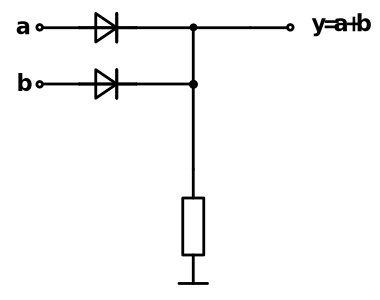
\includegraphics[width=0.3\linewidth]{diodovy_log_OR.pdf}}
        \subfloat[Součinový člen]{\label{ces:fig_D_AND}
          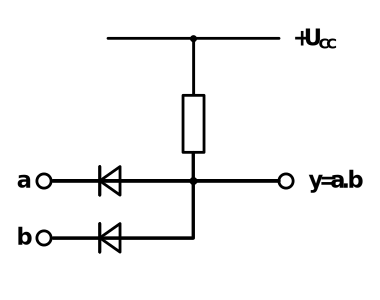
\includegraphics[width=0.3\linewidth]{diodovy_log_AND.pdf}}
        \caption{Diodová logika}
        \label{CES:fig_diodova_logika}
      \end{figure}
   \section{Unipolární digitální obvody}\label{CES:Unipolar_technology} 
  %-------------Přizpůsobení logických obvodů různých napěťových tříd-----------------------------
  % source: AN/Microchip/AN_3V_5V_Digital_Interfacing.pdf
  \newpage
  \section{Přizpůsobení logických obvodů různých napěťových tříd} %Digital Interfacing
    % When interfacing two devices that operate at different voltages, it is imperative to know the
    % output and input thresholds of both devices. Once these values are known, a technique can be
    % selected for interfacing the devices based on the other requirements of your application.
    % Table \ref{CES:tab_threshold} contains the output and input thresholds that will be used
    % throughout this document. When designing an interface, make sure to reference your
    % manufacturers data sheet for the actual threshold levels.
    Vyskytne-li se v číslicovém návrhu potřeba použít logická hradla z odlišných napěťových tříd,
    budeme postaveni před problém jejich vzájemného propojení zachovávající jejich funkčnost. Pro
    správnou volbu vhodného napěťového přizpůsobení logických hradel z různých rodin, je nutné znát
    nejen jejich rozhodovací napětí, ale také následující parametry, které jsou uvedeny v tabulce
    \ref{CES:tab_threshold} \cite[p.~22]{DS41285A}:
    
    \begin{itemize}\addtolength{\itemsep}{-0.5\baselineskip}
      \item maximální úroveň logické '0' na vstupu hradla - $\mathbf{V_{IL_{max}}}$
      \item minimální úroveň logické '1' na vstupu hradla - $\mathbf{V_{IH_{min}}}$
      \item maximální úroveň logické '0' na výstupu hradla - $\mathbf{V_{OL_{max}}}$
      \item minimální úroveň logické '1' na výstupu hradla - $\mathbf{V_{OH_{min}}}$
    \end{itemize}
    
    \begin{table*}
      \centering
      \begin{tabular}{|>{\columncolor{Tan}}l||c|c|c|c|}
        \hline
        \rowcolor{CornflowerBlue}{ }    & {$\mathbf{V_{OH_{min}}}$} & {$\mathbf{V_{OL_{max}}}$} & %
                                          {$\mathbf{V_{IH_{min}}}$} & {$\mathbf{V_{IL_{max}}}$} \\
        \hline
        \hline
        \texttt{5V TTL}                       
                    & 2.4V            & 0.5V       & 2.0V              & 0.8             \\
        \hline
        \texttt{3.3V LVTTL}          
                    & 2.4V            & 0.4V       & 2.0V              & 0.8             \\
        \hline
                    & 4.7V            & 0.5V       & 3.5V              & 1.5V            \\
        \multirow{-2}*{\texttt{5V CMOS}}      
                    & ($V_{CC}$-0.3V) &            & (0.7x$V_{CC}$)    & (0.3x$V_{CC}$)  \\
        \hline
                    
                    & 3.0V            & 0.5V       & 2.3V              & 1.0V            \\
        \multirow{-2}*{\texttt{3.3V LVCMOS}} 
                    & ($V_{CC}$-0.3V) &            & (0.7x$V_{CC}$)    & (0.3x$V_{CC}$)  \\
        \hline 
      \end{tabular}
      \caption{Rozhodovací úrovně napěťových tříd: \texttt{5V TTL}, \texttt{3.3V LVTTL}, 
                                                   \texttt{5V CMOS}, \texttt{3.3V
      LVCMOS}}\label{CES:tab_threshold}
    \end{table*}
    Úroveň logické nuly a jedničky na výstupu určuje konstrukce koncové části digitálního obvodu.
    Nejčastější provedení jsou na obr. \ref{ces:fig_digit_out_common}. Jsou-li různé digitální
    obvody připojeny na společnou sběrnici, může dojít k situaci, kdy některý z výstupních vývodů
    bude buzen vyšším napětím než je napájecí napětí příslušného obvodu. I v tomto případě výstupní
    část digitálního obvodu rozhoduje o výsledném chování. Shrňme základní vlastnosti technologií
    číslicových obvodů uvedených na obr. \ref{ces:fig_digit_out_common}:
    \begin{itemize}
      \item Bipolární koncový stupeň nedovoluje plný rozkmit výstupního signálu. Je-li obvod
            napájen \SI{5}{\volt}, je výstup při úrovni H limitován na $V_{CC}-2\times V_{BE}$(cca
            3.6V). To je hodnota, která na rozhraní \SI{3}{\volt} systému nezpůsobuje příliš velký
            napěťový rozdíl, a tedy proudu, tekoucímu z napájecího zdroje \SI{5}{\volt} systému do
            zdroje \SI{3}{\volt} systému.
      \item Výstupní napětí typické \texttt{CMOS} součástky se prakticky pohybuje v rozsahu
            \texttt{GND} - \texttt{VCC}.
      \item Některé součástky mají výstup typu \emph{open kolektor - OC} resp. \emph{open drain -
            OD}, tj. neexistuje vnitřní obvod, jenž by uvedl výstup do stavu H. K tomu je zapotřebí
            \emph{pull-up} rezistoru, který připojí výstup k napětí, které může být i vyšší než je
            napájecí - \texttt{VCC}. Očividně, tento způsob umožňuje relativně snadné rozhraní, ale
            pro dosažení vyšších rychlostí je nutné volit relativně malý odpor, což zvyšuje
            spotřebu.
      \item U \texttt{NMOS} stupně je podobně jako u bipolárního stupně výstupní napětí logické
            úrovně H omezeno úbytkem na kanálu horní NMOS tranzistoru na $V_{CC} - V_{TH}\simeq
            \SI{3.5}{\volt}$. Obvykle je tedy možné přímé řízení 3V systému.
    \end{itemize}

    \begin{figure}[ht!]
         \centering
         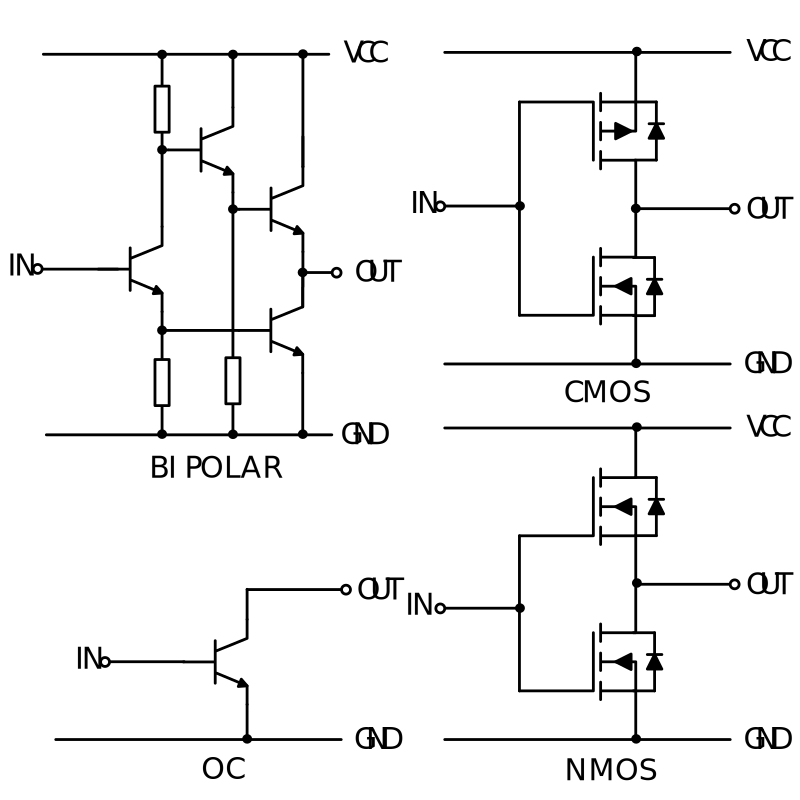
\includegraphics[width=0.7\linewidth]{digit_cir_output_common.pdf}
         \caption[Koncové stupně digitálních obvodů]
                 {Koncové stupně bipolárních, CMOS, NMOS obvodů a obvodů s otevřeným kolektorem 
                  \cite[p.~2]{AN240}}
         \label{ces:fig_digit_out_common}
    \end{figure}   
    
    % --------  Přizpůsobení: 3.3V -> 5V --------------------------- 
    \subsection{3.3V $\rightarrow$ 5V} %3.3V to 5V
      % The simplest and most desired way to connect a 3.3V output to a 5V input is by a direct
      % connection.  This can be done only if the following 2 requirements are met:
      Nejjednodušším a nejvíce žádoucím způsobem je přímé připojení 3.3V výstupu k 5V vstupu, což
      lze provést pouze v případě, že jsou splněny následující požadavky:
        \begin{itemize}\addtolength{\itemsep}{-0.5\baselineskip}
          \item $V_{OH}(3.3V)>V_{IH}(5V)$,
          \item $V_{OL}(3.3V)<V_{IL}(5V)$.
        \end{itemize}
      Hodnoty prahových napětí logické nuly a jedničky v předchozí tabulce \ref{CES:tab_threshold}
      dokládají, že v případě logiky \texttt{3.3V LVCMOS} a \texttt{5V TTL} je možné použít přímého
      připojení. 
      % An example of when this technique can  be used is interfacing a 3.3V LVCMOS output to a 5V
      % TTL input. From the values given in Table 4-1, it can clearly be  seen that both of these
      % requirements are met.

      % 3.3V LVCMOS VOH of 3.0 volts is greater than 5V TTL VIH of 2.0 volts and 3.3V LVCMOS VOL
      % of 0.5 volts is less than 5V TTL VIL of 0.8 volts.

      Pokud oba tyto požadavky nejsou splněny, je třeba použít na rozhraní obou logik
      přizpůsobovací obvody, popsané v následujících textu. 
      % When both of these requirements are  not met, some additional circuitry will be needed to
      % interface the two parts.

      \subsubsection{MOSFET Translator}
        \begin{figure}[ht!]
           \centering
           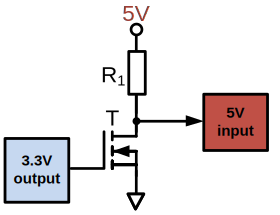
\includegraphics[scale=0.5]{level_shifting_MOSFET.pdf}
           \caption{3.3V $\rightarrow$ 5V: N-MOSFET}
           \label{CES:fig_shifting_MOSFET}
           \vspace*{-1\baselineskip}
        \end{figure}
        % In order to drive any 5V input that has a higher VIH than the VOH of a 3.3V CMOS part,
        % some additional circuitry is needed. A low-cost two component solution is shown in Figure
        % 6-1. When selecting the value for R1, there are two parameters that need to be considered;
        % the switching speed of the input and the current consumption through R1.
        Levné a jednoduché řešení problému vzájem\-ného přizpůsobení logických obvodů odliš\-ných
        napěťových tříd, pro které platí $V_{OH}(3.3V)<V_{IH}(5V)$ nabízí použití MOSFETu s
        prahovým napětím $$V_{GS_{th_{max}}}<V_{OH_{min}}.$$ Při výběru hodnoty $R_1$ je třeba vzít
        v úvahu:
        \begin{itemize}\addtolength{\itemsep}{-0.5\baselineskip}
          \item spínací rychlost vstupu,
          \item zvýšení spotřeby díky proudu přes rezistor $R_1$.
        \end{itemize}

        Při změně logické úrovně $'0'\rightarrow'1'$ na vstupu 5V logiky je nutné počítat se
        zpožděním, které je dáno časovou konstantu RC článku, tvořeného rezistorem $R_1$ a celkovou
        kapacitou na vstupu hradla. Důsledkem je tedy určitá minimální spínací perioda: 
        % When switching the input from a ‘0’ to a ‘1’, you will have to account for the time the
        % input takes to rise because of the RC time constant formed by R1, and the input
        % capacitance of the 5V input plus any stray capacitance on the board. The speed at which
        % you can switch the input is given by the following:
        $$T_{SW_{min}} = 3 \cdot R_1 \cdot C_{IN},$$ která je vyšší, čím nižší spotřeby se návrhář
        snaží dosáhnout ($R_1\uparrow$). Zpoždění při spínání $'1'\rightarrow'0'$ má příznivější
        hodnotu, neboť $R_{dsON}\ll R_1$.

        % Since the input and stray capacitance of the board are fixed, the only way to speed up
        % the switching of the input is to lower the resistance of R1. The trade-off of lowering
        % the resistance of R1 to get faster switching times is the increase in current draw when
        % the 5V input remains low. The switching to a ‘0’ will typically be much faster than
        % switching to a ‘1’ because the ON resistance of the N-channel MOSFET will be much smaller
        % than R1. Also, when selecting the N-channel FET, select a FET that has a lower VGS
        % threshold voltage than the VOH of 3.3V output.

      \subsubsection{Diodový Offset}
        Hodnoty vstupního prahového napětí \texttt{5V CMOS} a výstupní prahová napětí pro
        \texttt{3.3V LVTTL} a \texttt{LVCMOS} jsou uvedeny v tabulce \ref{CES:tab_diode_offset}
        % The inputs voltage thresholds for 5V CMOS and the output drive voltage for 3.3V LVTTL and
        % LVCMOS are listed in Table 7-1.
        \begin{table*}[t]
          \centering
          \begin{tabular}{|>{\columncolor{Tan}}l|c|c|c|}
            \hline
              \cellcolor{CornflowerBlue}                                   
                & \cellcolor{CornflowerBlue}\textbf{5V CMOS}       & 
              \cellcolor{CornflowerBlue} \textbf{3.3V LVTTL}               
                & \cellcolor{CornflowerBlue} \textbf{3.3V LVCMOS}  \\
              \multirow{-2}*{\cellcolor{CornflowerBlue}\texttt{Threshold}} 
                & \cellcolor{CornflowerBlue} IN 
                & \cellcolor{CornflowerBlue} OUT
                & \cellcolor{CornflowerBlue} OUT                   \\
            \hline\hline
               \texttt{High}                                               
                & $>3.5V$  & $>2.4V$ & $>3.0V$                     \\
               \texttt{Low}                                         
                & $<1.5V$  & $<0.4V$ & $<0.5V$                     \\
            \hline          
          \end{tabular}
          \caption{Přehled vstupní a výstupních prahový napětí různých logik, chceme-li ke vstupu
          \texttt{5V CMOS} připojit \texttt{3.3V LVTTL} nebo \texttt{3.3V LVCMOS.\cite{AN240}}}
          \label{CES:tab_diode_offset}
        \end{table*}

        \begin{figure}[ht!]
            \centering
            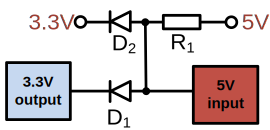
\includegraphics[scale=0.5]{level_shifting_diode_offset.pdf}
            \caption{3.3V $\rightarrow$ 5V: Diodový offset}
            \label{CES:fig_shifting_D_offset}
        \end{figure}

        Všimněme si, že obě prahová napětí vstupu \texttt{5V CMOS} logiky jsou o volt vyšší než u
        výstupu 3.3V logiky. Zapotřebí je tedy obvod, který zvyšuje vysokou a nízkou úroveň
        prahového napětí.
        % Note that both the high and low threshold input voltages for the 5V CMOS inputs are about
        % a volt higher than the 3.3V outputs. So, even if the output from the 3.3V system could be
        % offset, there would be little or no margin for noise or component tolerance. What is
        % needed is a circuit that offsets the outputs and increases the difference between the
        % high and low output voltages.

        Pokud bychom vytvořili posunutí o alespoň o 0.7V pro obě úrovně prahového napětí, dosáhli
        bychom vzájemného přizpůsobení. Obvod na obr. \ref{CES:fig_shifting_D_offset}, posuneme
        hodnotu nízké úrovně výstupního prahového napětí o úbytek v propustném směru diody $D_1$
        (typicky 0.7V), na 1.1V až 1.2V. Úroveň vysokého prahového napětí se nastavuje pomocí
        pull-up rezistoru a diody $D_2$ vázané na 3.3V napájení. Výstupní napětí je tedy také
        posunuto přibližně 0,7V nad 3,3V napájení, tj. na 4,0 až 4.1V, což je vysoko nad 3,5V
        prahem vstupu 5V CMOS logiky.

        % When output voltage specifications are determined, it is done assuming that the output is
        % driving a load between the output and ground for the high output, and a load between 3.3V
        % and the output for the low output. If the load for the high threshold is actually between
        % the output and 3.3V, then the output voltage is actually much higher as the load resistor
        % is the mechanism that is pulling the output up, instead of the output transistor.

        % If we create a diode offset circuit (see Figure 7-1), the output low voltage is increased
        % by the forward voltage of the diode D1, typically 0.7V, creating a low voltage at the 5V
        % CMOS input of 1.1V to 1.2V. This is well within the low threshold input voltage for the
        % 5V CMOS input. The output high voltage is set by the pull-up resistor and diode D2, tied
        % to the 3.3V supply. This puts the output high voltage at approximately 0.7V above the
        % 3.3V supply, or 4.0 to 4.1V, which is well above the 3.5V threshold for the 5V CMOS input
        \vskip2mm
        \begin{note}
          Aby obvod fungoval správně, musí být pull-up rezistor podstatně menší než vstupní odpor
          5V CMOS logiky, aby se zabránilo snížení výstupního napětí díky efektu vstupního
          odporového děliče a také musí být dostatečně velký, aby proud tekoucí do 3.3V napájení a
          výstupu hradla byl v mezích specifikace. 
          % For the circuit to work properly, the pull-up resistor must be significantly smaller
          % than the input resistance of the 5V CMOS input, to prevent a reduction in the output
          % voltage due to a resistor divider effect at the input. The pull-up resistor must also
          % be large enough to keep the output current loading on the 3.3V output within the
          % specification of the device.
        \end{note}

      \subsubsection{Komparátor}
        Základní funkce komparátoru je následující:        
        % The basic operation of the comparator is as follows:
        \begin{itemize}\addtolength{\itemsep}{-0.5\baselineskip}
          \item napětí na invertující (-) vstupu je větší než na neinvertujícím vstupu (+), výstup
                komparátoru se nastaví do nízké úrovně, 
                % When the voltage at the inverting (-) input is greater than that at the
                % non-inverting (+) input, the output of the comparator swings to Vss.
          \item je-li napětí na neinvertujícím vstupu (+) větší než na invertujícím vstupu (-),
                výstup komparátoru se nastaví do vysoké úrovně. %When the voltage at the
                % non-inverting (+) input is greater than that at the non-inverting (-)
                % input, the output of the comparator is in a high state.
        \end{itemize}

        \begin{figure}[ht!]
            \centering\vspace*{+1\baselineskip}
            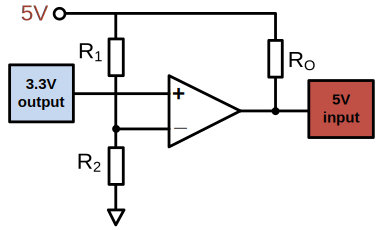
\includegraphics[scale=0.5]{level_shifting_COMP.pdf}
            \caption{3.3V $\rightarrow$ 5V: Komparátor; $R_1 = 1,8 k\Omega, R_2 = 1 k\Omega$}
            \label{CES:fig_shifting_COMP}           
        \end{figure}

        \textbf{Výpočet hodnoty odporu $R_1$ a $R_2$:}\newline
          Poměr R1 a R2 je závislý na napětí logické nuly a jedničky na výstupu hradla 3.3V logiky.
          Invertující vstup by měl být nastaven do poloviny mezi prahovými hladinami $V_{OL}$ a
          $V_{OH}$. Pro \texttt{LVCMOS} je toto napětí rovno $$1.75V = \frac{3V+0.5V}{2}.$$
          Budeme-li volit velikost $R_2$, pak hodnotu odporu $R_1$ snadno dopočítáme dle
          následující rovnice: $$R_1=R_2\left(\frac{5V}{1.75V}-1\right).$$ 
          % The ratio of R1  and R2  depends on the logic levels of the input signal. The inverting
          % input should be set to a voltage halfway between VOL and VOH for the 3.3V output. For
          % an LVCMOS output, this voltage is: $$1.75V = \frac{3V+0.5V}{2}.$$ Given that R1 and R2
          % are related by the logic levels:
          % $$R_1=R_2\left(\frac{5V}{1.75V}-1\right)$$ assuming a value of 1K for R2, R1 is 1.8K.

    % --------  Přizpůsobení: 5V -> 3.3V ---------------------------
    \subsection{5V $\rightarrow$ 3.3V} %5V to 3.3V
      \subsubsection{Přímé propojení}
        \begin{figure}[ht!]
            \centering
            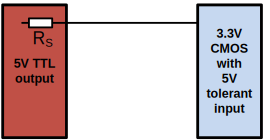
\includegraphics[scale=0.6]{direct_connect.pdf}
            \caption{5V $\rightarrow$ 3,3V: Přímé propojení}
            \label{CES:fig_dir_connect}
        \end{figure}

        Hradla napěťové třídy 5V mají výstupy s typickými prahovými hodnotami $V_{OH} = 4,7 V$,
        $V_{OL} = 0,4 V$ zatímco hradla 3.3V LVCMOS mají vstupy s prahovými hodnotami $V_{IH} =
        0,7\times V_{DD} $, $V_{IL} = 0,2\times V_{DD}$. Je-li tedy na 5V výstupu logická nula,
        bude také správně interpretována 3V vstupem, neboť platí $V_{OL} = 0,4 < V_{IL} = 0,8$. Ani
        v případě logické jedničky nevzniká žádný konflikt, neboť $V_{OH} = 4,7 > V_{IH} = 2,1$.
        Pokud je tedy 3V vstup 5V tolerantní, je možné přímé propojení, v opačném případě je třeba
        použít některou z následujících technik.
        % 5V outputs have a typical VOH of 4.7 volts and a VOL of 0.4 volts and a 3.3V LVCMOS input
        % will have a typical VIH of 0.7 x VDD and a VIL of 0.2 x VDD. When the 5V output is
        % driving low, there are no problems because the 0.4 volt output is less than in the input
        % threshold of 0.8 volts. When the 5V output is high, the VOH of 4.7 volts is greater than
        % 2.1 volt VIH, therefore, we can directly connect the 2 pins with no conflicts if the 3.3V
        % CMOS input is 5 volt tolerant. If the 3.3V CMOS input is not 5 volt tolerant, then there
        % will be an issue because the maximum volt specification of the input will be exceeded.

      \subsubsection{Diodový omezovač} %Diode Clamp
        Některé digitální obvody mají své vstupy chráněny vnitřními omezovacími diodami tzv.
        \texttt{diode clamp} (obr. \ref{CES:fig_int_clamp_D}). Proteče-li těmito diodami větší proud
        než udávají katalogové hodnoty, může dojít k poškození vstupu, nebo v lepším případě k
        efektu \texttt{latching-up}. Typický 5V výstup má kolem $10 \Omega$, proto chceme-li využít
        těchto diod, musíme přidat sériový odpor, jenž limituje velikost propustného proudu.
        Nepříjemným důsledkem je ovšem vzniklý RC článek se vstupní kapacitou hradla $C_L$, který
        snižuje rychlost. Není-li vstup takto chráněn je možné jej doplnit externí diodou dle obr.
        \ref{CES:fig_ext_clamp_D}.
        % Many manufacturers protect their I/O pins from exceeding the maximum allowable voltage
        % specification by using clamping diodes. These clamping diodes keep the pin from going
        % more than a diode drop below Vss and a diode drop above VDD. To use the clamping diode to
        % protect the input, you still need to look at the current through the clamping diode. The
        % current through the clamp diodes should be kept small (in the micro amp range). If the
        % current through the clamping diodes gets too large, then you risk the part latching up.
        % Since the source resistance of a 5V output is typically around 10 ohms, an additional
        % series resistor is still needed to limit the current through the clamping diode as shown
        % Figure 10-1. The consequence of using the series resistor is it will reduce the speed at
        % which we can switch the input because the RC time constant formed the capacitance of the
        % pin (CL).
       \begin{figure}[ht!]
         \centering
         \begin{tabular}{c}
           \subfloat[Vnitřními omezovací diody]{\label{CES:fig_int_clamp_D}
             \includegraphics[width=0.3\textwidth]{CES_clamp_diodes_input.png}}        \\
           \subfloat[Externí omezovací dioda]{\label{CES:fig_ext_clamp_D}     
             \includegraphics[width=0.3\textwidth]{CES_ext_clamp_diodes_input.png}}
         \end{tabular}  
         \caption{5V $\rightarrow$ 3,3V: Použití omezovacích diod pro ochranu vstupu integrovaného
                  obvodu}
         \label{CES:fig_clamp_diodes}
       \end{figure} 
        % One problem with using a diode clamp is that it injects current onto the 3.3V power
        % supply. In designs with a high current 5V outputs, and lightly loaded 3.3V power supply
        % rails, this injected current can float the 3.3V supply voltage above 3.3V. To prevent
        % this problem, a transistor can be substituted which routes the excess output drive
        % current to ground instead of the 3.3V supply.
          
        Dalším problémem je proud, injektovaný z 5V výstupu skrz omezovovací diodu do 3.3V
        napájení. Tento proud může způsobit zvýšení napájecího napětí 3.3V obvodů, což může vést k
        jejich zničení. Proto lze s výhodou použít PNP tranzistor zapojený dle obr.
        \ref{CES:fig_bjt_clamp}.
        
        \begin{figure}[ht!]
          \centering
          \includegraphics[scale=0.5]{CES_ext_clamp_bjt_input.png}
          \caption{5V $\rightarrow$ 3,3V: Active clamp - Přechod báze-emitor funguje jako omezovací
                   dioda, ovšem s tím rozdílem, že jen malé procento celkového proudu z 5V výstupu
                   teče do 3.3V napájení. Převážná část teče kolektorem do země. Poměr bázového a
                   kolektorového proudu je určen proudovým zesílením tranzistoru, které je typicky
                  10 až 400}
          \label{CES:fig_bjt_clamp}
        \end{figure}              
       
      \subsubsection{Napěťový dělič} %Resistor divider
        A simple resistor divider can be used to reduce the output of a 5V device to levels
        appropriate for a 3.3V device input. An equivalent circuit of this interface is shown in
        Figure \ref{CES:fig_res_divider}.
        \begin{figure}[ht!]
          \centering
          \includegraphics[scale=0.4]{CES_ext_res_divider.png}
          \caption{5V $\rightarrow$ 3,3V: napěťový děliš}
          \label{CES:fig_res_divider}
        \end{figure}
        Typically, the source resistance, $R_S$, is very small (less than 10 ohms) so its affect on
        $R_1$ will be negligible provided that $R_1$ is chosen to be much larger than $R_S$. At the
        receive end, the load resistance, $R_L$, is very large (greater than 500 k ohms) so its
        affect on $R_2$ will be negligible provided that $R_2$ is chosen to be much less than
        $R_L$.
        
        There is a trade-off between power dissipation and transition times. To keep the power
        requirements of the interface circuit at a minimum, the series resistance of $R_1$ and
        $R_2$ should be as large as possible. However, the load capacitance, which is the
        combination of the stray capacitance, $C_S$, and the 3.3V device input capacitance, $C_L$,
        can adversely affect the rise and fall times of the input signal. Rise and fall times can
        be unacceptably long if $R_1$ and $R_2$ are too large.
        
        Neglecting the affects of $R_S$ and $R_L$, the formula for determining the values for $R_1$
        and $R_2$ is given by Equation \ref{CES:eq_res_divider}.
        \begin{align}\label{CES:eq_res_divider}
          \frac{V_S}{R_1+R_2} &= \frac{V_L}{R_2}           \nonumber \\
                          R_1 &= \frac{(V_S-V_L)}{V_L}R_2  \nonumber \\
                          R_1 &= 0,515\cdot R_2
        \end{align}      
        The formula for determining the rise and fall times is given in Equation
        \ref{CES:eq_res_divider_time}. For circuit analysis, the Thevenin equivalent is used to
        determine the applied voltage, $V_A$, and the series resistance, $R$.
        The Thevenin equivalent is defined as the open circuit voltage divided by the short circuit
        current. The Thevenin equivalent, $R$, is determined to be $0.66\cdot R_1$ and the Thevenin
        equivalent, $V_A$, is determined to be $0.66\cdot V_S$ for the circuit shown in  Figure
        \ref{CES:fig_res_divider} according to the limitations imposed by Equation
        \ref{CES:eq_res_divider_time}.
        \begin{equation}\label{CES:eq_res_divider_time}
          t = - R\cdot C \cdot \ln\left(\frac{V_F-V_A}{V_I-V_A}\right)
        \end{equation}  
        kde $t$ = Rise or Fall time, $R = 0.66\cdot R_1$, $C = C_S+C_L$, $V_I$ = Initial voltage on
        $C$ ($V_L$), $V_F$ = Final voltage on $C$ ($V_L$), $V_A$ = Applied voltage ($0.66\cdot V_S$). 
        \begin{example} As an example, suppose the following conditions exist:
          \begin{itemize}\addtolength{\itemsep}{-0.5\baselineskip}
            \item Stray capacitance = 30 pF,
            \item Load capacitance = 5 pF,
            \item Maximum rise time from 0.3V to 3V ≤ 1 μS
            \item Applied source voltage Vs = 5V
          \end{itemize}
          Solve Equation \ref{CES:eq_res_divider_time} for $R$:  
          \begin{equation*}
            R = - \dfrac{t}{C\cdot\ln\dfrac{V_F-V_A}{V_I-V_A}}
          \end{equation*}   
          Substitute values:
          \begin{equation*}
            R = - \dfrac{10\cdot10^{-7}}{35\cdot10^{-12}\cdot
                  \ln\dfrac{3-0.66\cdot5}{0.3-0.66\cdot5}}
          \end{equation*}               
          Thevenin equivalent maximum R: $$R = 12408$$
          Solve for maximum $R_1$ and $R_2$:
          \begin{alignat}{3}
            & R_1 &&= 0.66\cdot R  \qquad &&R_2 = \frac{R_1}{0.515}  \\
            & R_1 &&= 8190         \qquad &&R_2 = 15902 
          \end{alignat}          
        \end{example} 
                   
      \subsubsection{Level translator} %Level translator
        While level translation can be done discretely, it is often preferred to use an integrated
        solution. Level translators are available in a wide range of capabilities. There are
        unidirectional and bidirectional configurations, different voltage translations and
        different speeds, all giving the user the ability to select the best solution. 
        \begin{figure}[ht!]
          \centering
          \begin{tabular}{c}
            \subfloat[SPI sběrnice]{\label{CES:fig_level_translator1}
              \includegraphics[width=0.9\linewidth]{CES_ext_level_translator1.png}}           \\
            \subfloat[I2C sběrnice]{\label{CES:fig_level_translator2}
              \includegraphics[width=0.9\linewidth]{CES_ext_level_translator2.png}}
          \end{tabular}  
          \caption{5V $\rightarrow$ 3,3V: Board-level communication between devices (e.g., MCU to
                   peripheral) is most often done by either SPI or I2C. For SPI, it may be
                   appropriate to use a unidirectional level translator and for I2C, it is necessary
                   to use a bidirectional solution.}
          \label{CES:fig_level_translator}
        \end{figure}           
      
} % tikzset
%---------------------------------------------------------------------------------------------------
\printbibliography[title={Seznam literatury}, heading=subbibliography]
\addcontentsline{toc}{section}{Seznam literatury}
%  \input{../src/CES/chap/Basic_MCU_Arch.tex}
%  % !TeX spellcheck = cs_CZ
%{\tikzset{external/prefix={tikz/CES/}}
% \tikzset{external/figure name/.add={ch02_}{}}
%---------------------------------------------------------------------------------------------------
% file Basic_MCU_Arch.tex
%---------------------------------------------------------------------------------------------------
\lstset{ %
  language={[x86masm]Assembler},         % choose the language of the code
  inputencoding=latin1,
  extendedchars=true,
  showspaces=false,                      % show spaces everywhere adding particluar undescores, it  
                                         % overrides 
                                         % “showstringspaces”
  showstringspaces=false,                % underline spaces within strings only
  basicstyle=\footnotesize\ttfamily,     % the size of the fonts that are used for the code
%  backgroundcolor=\color{White},        % choose the background color. You must add  
                                         % \usepackage{color}
  breaklines=true,                       % sets automatic line breaking
  breakatwhitespace=true,                % sets if automatic breaks should only happen at whitespace
  showspaces=false,                      % show spaces adding particular underscores
  showstringspaces=true,                 % underline spaces within strings
  showtabs=true,                         % show tabs within strings adding particular underscores
  frame=none,                            % adds a frame around the code - none, single
  tabsize=2,                             % sets default tabsize to 2 spaces
  captionpos=b,                          % sets the caption-position to bottom
  numbers=left,                          % where to put the line-numbers -none, left, right
  numberstyle=\tiny\color{lstnumcolor},  % the size of the fonts that are used for the line-numbers
  numbersep=5pt,                         % how far te line-number are from the code
  stepnumber=1,                          % the step between two line-numbers. If it's 1 each line
                                         % will be numbered
  xleftmargin=3em,                       % adjust left margin
  commentstyle=\color{help}\textit,      % comment style
  keywordstyle=\color{keyword}\textbf,   % keyword style
  morekeywords={ADDC, ASHR, SUBB,CLR,    % if you want to add more keywords to the set
    MAC,  MULS, DIVS, BSET, BCLR, BCPL, 
    BAND, BOR,  BXOR, BCMP, TRL,  EX,  BMOV,
    JCC,  BCC,  DJNZ, RETI, JSR,  CSP, LDR},
  literate= %
    {á}{{\'a}}1  {é}{{\'e}}1     {í}{{\'i}}1   {ó}{{\'o}}1   {ú}{{\'u}}1
    {Á}{{\'A}}1  {É}{{\'E}}1     {Í}{{\'I}}1   {Ó}{{\'O}}1   {Ú}{{\'U}}1
    {à}{{\`a}}1  {è}{{\`e}}1     {ì}{{\`i}}1   {ò}{{\`o}}1   {ù}{{\`u}}1
    {À}{{\`A}}1  {È}{{\'E}}1     {Ì}{{\`I}}1   {Ò}{{\`O}}1   {Ù}{{\`U}}1
    {ä}{{\"a}}1  {ë}{{\"e}}1     {ï}{{\"i}}1   {ö}{{\"o}}1   {ü}{{\"u}}1
    {Ä}{{\"A}}1  {Ë}{{\"E}}1     {Ï}{{\"I}}1   {Ö}{{\"O}}1   {Ü}{{\"U}}1
    {â}{{\^a}}1  {ê}{{\^e}}1     {î}{{\^i}}1   {ô}{{\^o}}1   {û}{{\^u}}1
    {Â}{{\^A}}1  {Ê}{{\^E}}1     {Î}{{\^I}}1   {Ô}{{\^O}}1   {Û}{{\^U}}1
    {œ}{{\oe}}1  {Œ}{{\OE}}1     {æ}{{\ae}}1   {Æ}{{\AE}}1   {ß}{{\ss}}1
    {ç}{{\c c}}1 {Ç}{{\c C}}1    {ø}{{\o}}1    {å}{{\r a}}1  {Å}{{\r A}}1
    {€}{{\EUR}}1 {£}{{\pounds}}1 {ř}{{\v{r}}}1 {ž}{{\v{z}}}1 {č}{{\v{c}}}1
    {ě}{{\v{e}}}1
}
%================== Kapitola: Základy mikroprocesorové techniky====================================
%\setchaptertoc
\chapter{Historie mikroprocesorové techniky}
\minitoc
    \subsection{Vývoj mikroprogramových řadičů: od mainframu EDSAC k moderním 
                 mikroprocesorům}\hypertarget{MIT:sec_003}
      Na princip funkce mikrořadiče řízeného pomocí mikroprogramů, jenž byl popsaný v kapitole 
      \ref{ces:IchapIVsecIIssecI}, se můžeme dívat jako na zobecnění idey programování počítačů 
      pomocí instrukcí uložených v operační paměti. V samých počátcích vývoje výpočetní techniky, 
      konkrétně u takzvané nulté generace (zhruba do roku 1947) a první generace (cca roky 1946 až 
      1958) počítačů, se totiž algoritmy nevyjadřovaly pomocí instrukcí tvořících ucelené programy, 
      které by byly uloženy do paměti. Namísto toho byl algoritmus „zadrátován“ (obr. 
      \ref{MIT:fig_eniac}) takovým způsobem, že se pomocí vodičů umístěných většinou na spínacích 
      panelech vzájemně propojovaly jednotlivé moduly počítače – sčítačky, pracovní registry, 
      řadiče paměti, vstupní prvky atd. Navíc se u některých specializovaných počítačů používaných 
      za druhé světové války pro luštění šifer nedal algoritmus vůbec měnit – počítač stále 
      prováděl stejné výpočty, ovšem s různými daty. Tato konstrukce počítačů odpovídala dobové 
      technologii, které se používala především v telefonních ústřednách s ručním přepojováním 
      hovorů, semaforech nebo například pro ovládání výtahů.
      
      \begin{figure}[ht!]   %\ref{MIT:fig_eniac}
        \centering
        \includegraphics[width=0.9\linewidth]{eniac.jpg}
        \caption{Způsob programování elektronického počítače \Eniac (\emph{Electronic Numerical 
                 Integrator And Computer}) pomocí vzájemného propojování jednotlivých modulů 
                 přepojováním kabelů mezi jednotlivými funkčními moduly. Kredit: Columbia 
                 university}
        \label{MIT:fig_eniac}
      \end{figure}
      
      \subsubsection{Von Neumannova architektura programovatelného počítače}
        Ovšem již v polovině čtyřicátých let minulého století přišel \wikiNeumann s převratnou 
        myšlenkou – libovolný algoritmus nemusí být přímo „zadrátován“ v počítači, ale může být 
        zapsán ve formě programu složeného ze sekvence instrukcí, které mohou být uloženy v paměti 
        počítače naprosto stejným způsobem, jako zpracovávaná data; viz též dnes již klasické von 
        Neumannovo dílo \wikiEDVAC vydané v roce 1945. Právě díky této myšlence vznikly první 
        skutečné procesory s instrukčními sadami, děrné štítky se začaly používat mj. i pro uložení 
        programů a navíc se otevřela cesta k dalšímu zobecnění: programy začaly být asi o deset let 
        později vytvářeny ve vyšších programovacích jazycích, přičemž překlad prováděl jiný program 
        (algoritmus) nazývaný překladač (dnes bereme překladače jako zcela běžnou věc, ale idea, že 
        překladač je sám o sobě taktéž algoritmem, byla v době její implementace chápána jako malá 
        revoluce). Toto dvojí zobecnění práce univerzálního programovatelného počítače nebylo 
        dodnes překonáno a je na něm založena i moderní výpočetní technika a informatika.
        
        Architektura počítačů navržená John von Neumannem byla založena na \emph{centrální 
        procesorové jednotce} rozdělené na \emph{aritme\-ticko-logickou jednotku} a 
        \emph{řadič}, 
        který na základě instrukcí čtených z operační paměti řídil všechny další moduly počítače 
        (vstupně-výstupní zařízení, aritmeticko-logickou jednotku, operační paměť). Nikde ovšem 
        nebylo přesně specifikováno, jakým způsobem má být řadič, jakožto „mozek“ počítače, 
        implementován. V prvních mainframech založených na myšlence Johna von Neumanna se tedy 
        uplatňovaly obvodové řadiče. Tyto řadiče byly dostatečně rychlé a nevyžadovaly ke své 
        činnosti prakticky žádné paměťové prvky (většinou jen čítač či posuvný registr), ovšem 
        přinášely i některé nevýhody. Jednou z poměrně závažných nevýhod byla velká složitost 
        obvodového řadiče v případě, že se používala komplexnější instrukční sada (\texttt{CISC}). 
        Poněkud paradoxně se právě složité instrukční sady začaly v padesátých letech minulého 
        století stále více používat, zejména na mainframech druhé generace. A právě tehdy se začala 
        prakticky realizovat myšlenka \emph{mikroprogramování}.
      
      \subsubsection{EDSAC – první počítač se skutečným mikroprogramovým řadičem}
        Myšlenka mikroprogramování vznikla již v roce 1951, kdy ji ve svých článcích představil sir 
        \wikiEWilkes (titul sir získal Wilkes právě za svoji dlouholetou práci v oboru 
        \texttt{IT}). Idea mikroprogramování spočívala v zobecnění konstrukce centrální procesorové 
        jednotky (\texttt{CPU}) takovým způsobem, že strojové instrukce byly rozkládány na sekvenci 
        řídicích signálů pomocí mikroprogramu uloženého v paměti typu \texttt{ROM} s velmi rychlou 
        dobou přístupu. Vzhledem ke stavu technologie v roce 1951 samozřejmě V. Wilkes nemohl 
        použít klasický čip s \texttt{ROM}, v němž jsou bity trvale zaznamenány s použitím 
        poslední, zákazníkem definované masky při výrobě čipu. Namísto toho Wilkes navrhoval použít 
        matici navzájem kolmých vodičů, v níž by byla bitová jednička „zaznamenána“ pomocí diody 
        spojující jeden vodorovný a jeden svislý vodič (vodivou kovovou spojku nelze použít, 
        protože by se do matice nepřímo zapsaly i falešné jedničky).
        
        \begin{figure}[ht!]   %\ref{MIT:fig_edsac}
          \centering
          \includegraphics[width=0.95\linewidth]{EDSAC.jpg}
          \caption{\wikiEDSAC (Electronic Delay Storage Automatic Calculator) byl britský počítač z 
                   poloviny 20. století. Tento počítač, inspirovaný John Von Neumannovým dokumentem 
                   First Draft of a Report on the EDVAC, sestavil Maurice Wilkers a jeho tým na 
                   Univerzitě v Cambridgi v Anglii. EDSAC byl první v praxi využitý počítač 
                   pracující s uloženým programem. Kredit: Wikipedia, Root.cz}
          \label{MIT:fig_edsac}
        \end{figure}
        
        Na zpočátku pouze teoretickou práci M. V. Wilkese o několik let později navázali William 
        Renwick a \wikiWheeler, kteří v roce 1957 sestrojili první skutečný počítač založený na 
        mikroprogramovém procesoru. Vzhledem k tomu, že diodová matice navržená Wilkesem by byla 
        příliš rozměrná pro počítač s velkou instrukční sadou (diodami jsou zde samozřejmě myšleny 
        diskrétní elektronické součástky, i když se v roce 1957 již pomalu schylovalo k výrobě 
        prvních prototypů integrovaných obvodů), použili W. Renwick a D. Wheeler namísto diod 
        feritovou paměť, což bylo ve svém důsledku velmi zajímavé, protože se obsah této paměti dal 
        přeprogramovat a tím pádem bylo možné i měnit instrukční sadu počítače. První prototyp 
        tohoto stroje byl nazván \texttt{EDSAC 1½} a používal pro uložení mikroinstrukcí feritovou 
        paměť s maticí o velmi malých rozměrech 6×8 feritových jader – tento počítač ovšem 
        neobsahoval celou instrukční sadu. Finální podoba počítače z roku 1958, jež nesla název 
        \texttt{EDSAC 2}, měla již paměťovou matici o rozměrech 32×32 feritových jader, což již 
        umožnilo implementaci plnohodnotné instrukční sady za použití mikrokódů.
    
%} % tikzset
%---------------------------------------------------------------------------------------------------
\printbibliography[title={Seznam literatury}, heading=subbibliography]
\addcontentsline{toc}{section}{Seznam literatury}
}
{
% DEBUG was off
%======================= Kapitola01: Číslicové systémy a signály ===================================
  % !TeX spellcheck = cs_CZ
{\tikzset{external/prefix={tikz/CES/}}
 \tikzset{external/figure name/.add={ch01_}{}}
%---------------------------------------------------------------------------------------------------
% file cis_sig_sys.tex
%---------------------------------------------------------------------------------------------------
\definecolor{Gray}{gray}{0.9}
%===================== Kapitola: Číslicové systémy a signály========================================
\chapter{Číslicové systémy a signály}  
\minitoc

  \section{Co je číslicový systém}
    V číslicovém systému se pracuje se signály, které mají jen konečný počet diskrétních hodnot. 
    Tím se liší od systémů analogových, u kterých jsou signály spojité, tj. mohou ve vymezeném 
    rozsahu nabývat nekonečný počet hodnot. V číslicovém systému může i čas být veličinou 
    diskrétní, tj. signály se mohou měnit jen v určitých okamžicích. Takovéto číslicové systémy
    se pak nazývají \textbf{synchronní} - na rozdíl od systémů \textbf{asynchronních}, u kterých ke 
    změnám signálů může docházet kdykoliv. Synchronní systémy jsou podstatně častější, neboť 
    existence přesně stanovených okamžiků změn signálů zavádí "pořádek" do časování signálů v 
    systému a tím usnadňuje jeho konstrukci i výrobu v podobě integrovaných obvodů. Přesné
    časování je zajištěno hodinovými (taktovacími) impulsy, což je velmi významný signál systému \cite[s.~14]{Pinker2006}.
  
    Číslicové systémy se dělí na dvě skupiny
    \begin{itemize}\addtolength{\itemsep}{-0.5\baselineskip}
      \item \textbf{kombinační systémy},
      \item \textbf{sekvenční systémy}.
    \end{itemize}
    U kombinačních systémů jsou výstupní signály závislé pouze na momentálních vstupních signálech. 
    U sekvenčních systémů jsou výstupní signály závislé nejen na momentálních vstupních signálech, 
    ale i na vstupních signálech v minulosti. Systém tedy má \emph{vnitřní paměť}.
    
    \subsection{Dvojstavové signály}
      Jak již bylo řečeno, číslicové signály mají jen konečný počet diskrétních hodnot. V naprosté 
      většině jrou to právě jen dvě hodnoty. Dvouhodnotové nebo dvoustavové signály snižují nároky 
      na výrobní tolerance. Bylo tak možné zavést výrobní postupy, které umožňují hromadnou a 
      levnou výrobu součástek. 
      
      Předpokládejme, že číslicové součástky jsou napájeny kladným napětím $+U_{CC}$. Jedna hodnota 
      bude vyjádřena nižším napětím, druhá vyšším napětím. Dvě možné hodnoty signálu označíme jako 
      '0' a '1' (v souladu se značením v \hyperref[CES:basic_bool_alg]{Boolově algebře}).
     
  \section{Kombinační logické funkce}
    Základním pojmem při úvahách o kombinačních systémech představuje pojem kombinační logická
    funkce.  \emph{Kombinační logická funkce} je pravidlo přiřazující každé kombinaci hodnot
    \texttt{0} a \texttt{1} přiřazených vstupním proměnným z definičního oboru funkce jedinou
    hodnotu výstupní proměnné. Pro daný počet vstupních proměnných je těchto funkcí konečný počet.
    Kombinační logické funkce mohou být úplně nebo neúplně určené.  \emph{Úplně určená kombinační
    logická funkce} je taková funkce, jejíž definiční obor zahrnuje všechny kombinace vstupních
    proměnných. U \emph{neúplně určené kombinační logické funkce} její definiční obor nezahrnuje
    některé tyto kombinace. Kombinací se zde rozumí kombinace hodnot  \texttt{0} a \texttt{1}
    přiřazených jednotlivým vstupním proměnným. Úplně určeným funkcím se někdy říká úplné funkce,
    funkcím neúplné určeným pak neúplné funkce.
   
  \subsection{Realizace kombinačních logických funkcí} 
    Nejčastěji se v digitální technice setkáme s těmito způsoby realizace kombinační logické funkce:
      \begin{itemize}\addtolength{\itemsep}{-0.5\baselineskip}
        \item pomocí digitálních integrovaných obvodu typu \texttt{NAND}, \texttt{NOR} (popř.   
              \texttt{AND}, \texttt{OR}) a dalších obvodů realizujících základní kombinační logické 
              funkce - např. \texttt{AND-OR-INVERT}, \texttt{EX-OR} atd.,
        \item pomocí multiplexeru a demultiplexeru,
        \item pomocí speciálních kombinačních integrovaných obvodu (převodníky kódu, generátory    
              parity, sčítačky, násobičky a podobně - sem patří i použití multiplexeru a 
              demultiplexeru),
        \item pomocí pamětí (např. \texttt{PROM} a \texttt{EEPROM}),
        \item pomocí programovatelných logických obvodu (\texttt{PLD}). 
      \end{itemize}
      
      \subsubsection{Použití multiplexerů a demultiplexerů k realizaci kombinačních logických funkcí}
   
  \subsection{Základní pravidla Booleovy algebry}\label{CES:basic_bool_alg}
    Nejdůležitější postuláty:
    \begin{align}
       \shortintertext{Univerzální vazba:}
         x + 0 = x \quad x\cdot 0 = 0 &|  x + 1 = 1 \quad x\cdot 1 = 1                         \\
       \shortintertext{Doplňek}
         x + \overline{x} = 1         &|  x\cdot\overline{x} = 0                               \\
       \shortintertext{Idempotence}
         x +x = x                     &|  x\cdot x = x      
      \label{CES:postul_Idemp}
    \end{align}
  \subsection{Zjednodušování zápisu logické funkce}
     Logická funkce vyjádřená úplnou součtovou (disjunktivní) nebo součinovou (konjuktivní) formou 
     z pravdivostní tabulky není jediným možným zápisem logické funkce. Dá se většinou nalézt 
     jednodušší algebraický zápis, z něhož můžeme předpokládat, že povede na realizaci méně 
     složitého číslicového obvodu. Který ze zápisů logické funkce povede na minimální složitost 
     obvodu závisí nejen na použitých logických členech, ale též na dalších kritériích: zpoždění, 
     spotřeba obvodu, jeho spolehlivost, potlačení hazardních stavů, atd. První metodou je 
     \emph{algebraická minimalizace}, 
     
    \subsubsection{Karnaughova metoda minimalizace pomocí mapy}  
      Jednou z možností grafického zápisu logické funkce je mapa. Nejpoužívanější je 
      \textbf{Karnaughova mapa} (čti ''karnau''). Mapa je uspořádána do čtverce či obdélníka a to 
      tak, že \emph{sousední pole} se liší vždy jen v jedné proměnné.
      \begin{table}
        \centering
        \begin{tabular}{lr}
          \begin{tabular}[t]{r|cccc|c}
             \rowcolor{Gray}{\textbf{Index}}& {$x_4$} & {$x_3$} & {$x_2$} & {$x_1$} & {$f$} \\
             \hline
             0&0&0&0&0&1\\
             1&0&0&0&1&1\\
             2&0&0&1&0&1\\
             3&0&0&1&1&0\\
             4&0&1&0&0&0\\
             5&0&1&0&1&1\\
             6&0&1&1&0&1\\
             7&0&1&1&1&0\\
             8&1&0&0&0&0\\
             9&1&0&0&1&1\\
            10&1&0&1&0&1\\
            11&1&0&1&1&0\\
            12&1&1&0&0&0\\
            13&1&1&0&1&1\\
            14&1&1&1&0&1\\
            15&1&1&1&1&0\\
          \end{tabular}
        \end{tabular}
        \caption[Pravdivostní tabulka logické funkce]{Pravdivostní tabulka logické funkce čtyř 
        proměnných, kterou se pokusíme vyjádřit také pomocí Karnaughovy mapy}
        \label{CES:tab_true1}
      \end{table} 

      Mapu chápáme jako uspořádaný zápis pravdivostní tabulky vzniklou transformací řádku tabulky 
      na jedno pole mapy \cite[s.~25]{Podlesak1994}. Tedy, každé pole mapy jednoznačně odpovídá 
      určité kombinaci všech proměnných. Nalézá-li se pole pod pruhem vyznačeným u proměnné, bude 
      tato proměnná nenegovaná. Nalézá-li se mimo pruh, bude proměnná negovaná. Tak např.
      pole označené jako x v mapě pro tři proměnné bude odpovídat kombinaci 
      $x_1\overline{x_2}\overline{x_3}$. Jak je názorně vidět, z pravdivostní tabulky funkce lze 
      snadno sestavit její mapu a naopak. Řádkům pravdivostní tabulky, ve kterých je
      funkční hodnota 1, odpovídají pole mapy s vepsanou jedničkou; obdobně to platí i pro nuly. V 
      mapě lze znázornit i neurčené stavy prázdným políčkem (nebo pomlčkou) 
      \cite[s.~219]{Wakerly1999}.
       
      \begin{figure}[hb!]
          \centering
          \karnaughmap{2}{$f(x_1,x_2):$}{{$x_2$}{$x_1$}}{1010}{}
          \karnaughmap{3}{$f(x_1,x_2,x_3):$}{{$x_3$}{$x_2$}{$x_1$}}{1x      }{}  
          \karnaughmap{4}{$f(x_1,x_2,x_3,x_4):$}{{$x_4$}{$x_3$}{$x_2$}{$x_1$}}{1010011001100110}{}        
        \caption{Příklad Karnaughovy mapy pro dvě, tři a čtyři proměnné}\label{CES:karnaugh_234}
      \end{figure}     
      
      Přiřazení kombinací hodnot vstupních proměnných (součinů) jednotlivým polím mapy se označuje 
      jako \emph{kódování}. Řádky i sloupce Karnaughovy mapy jsou kódovány \textbf{Grayovým kódem}. 
      Základní vlastností Grayova kódu je to, že sousední slova konstantí délky se liší pouze v 
      jedné proměnné. Tuto vlastnost splňuje i první a poslední kódové slovo (kód je uzavřen sám
      do sebe) viz \ref{CES:BCD_Gray_c}. Právě tato vlastnost je využita při konstrukci Karnaughovy 
      mapy - souřadnice polí jsou uspořádány tak, že u sousedních polí se liší jen v jedné 
      proměnné. Tudíž geometricky sousedící pole jsou sousední i v algebraickém smyslu (liší se v 
      jediné proměnné).  
      
     \begin{table}[ht!] 
       \centering 
       \begin{tabular}{|c|c|c|}
         \hline
         \rowcolor{CornflowerBlue}{\textbf{Číslo}}  & \textbf{Binární kód} & \textbf{Grayův kód} \\
         \rowcolor{CornflowerBlue}{ }               &     {$x_1,x_2,x_3$}  & {$x_1,x_2,x_3$}     \\
          \hline\hline  
             \cellcolor[gray]{0.9}0                 & 000                  & 000               \\
          \hline       
             \cellcolor[gray]{0.9}1                 & 001                  & 001               \\
          \hline  
             \cellcolor[gray]{0.9}2                 & 010                  & 011               \\
          \hline  
             \cellcolor[gray]{0.9}3                 & 011                  & 010               \\
          \hline  
             \cellcolor[gray]{0.9}4                 & 100                  & 110               \\
          \hline         
             \cellcolor[gray]{0.9}5                 & 101                  & 111               \\
          \hline  
             \cellcolor[gray]{0.9}6                 & 110                  & 101               \\
          \hline  
             \cellcolor[gray]{0.9}7                 & 111                  & 100               \\
          \hline
       \end{tabular}
       \caption{Binární a Grayův kód pro tři proměnné}
       \label{CES:BCD_Gray_c}    
     \end{table}       
      
     Každé pole s hodnotou 1 odpovídá \textbf{mintermu} z pravdivostní tabulky. Sousední pole tedy 
     odpovídají mintermům lišícím se jen jednou proměnnou, a ty lze spojovat do 
     \textbf{implikantů}. Sousední jsou i pole na okrajích mapy, neboť i ta se liší
     jen v jedné proměnné (konce řádek, konce sloupců a rohy mapy). Spojováním výrazů sousedních 
     políček provádíme minimalizaci, která díky jasnému geometrickému postupu vyhýbá 
     problematickému hledání těchto součtů nebo součinů. 
     
     Spojování polí se vyznačí \textbf{smyčkou}. Pole po dvojicích sousední lze spojovat do větších 
     smyček, ty opět do větších atd. Každá smyčka tedy musí mít stranu dlouhou právě $2^k$ polí, 
     kde $k$  je celé kladné číslo. Smyčky zahrnují 2 pole, 4 pole, 8 polí, atd. Každá smyčka v 
     mapě odpovídá implikantu funkce. Princip minimalizace spočívá v pokrytí všech     
     jedniček\footnote{nul pro součinovou formu} (a libovolných neurčených stavů) soustavou smyček 
     pro součtovou formu, přičemž:
     \begin{itemize}\addtolength{\itemsep}{-0.5\baselineskip}
       \item smyčky musí být co možná největší,
       \item smyček musí být co nejmenší počet.       
     \end{itemize}     
     Tento princip je ilustrován na následující mapě funkce čtyř proměnných. Jako příklad vezmeme 
     funkci definovanou pravdivostní tabulkou \ref{CES:tab_true1}. Odpovídající Karnaughova mapa 
     pro čtyři proměnné je na obrázku \ref{CES:karnaugh_234}. Základní součtový tvar této funkce je 
     dán rovnici:     
     \begin{align}
        f(x_1, x_2, x_3, x_4) 
          &= \overline{x_1x_2x_3x_4} + \overline{x_1}x_2\overline{x_3x_4} +           \nonumber \\
          &+ x_1\overline{x_2}x_3\overline{x_4} + \overline{x_1}x_2x_3\overline{x_4}+ \nonumber \\ 
          &+ x_1\overline{x_2x_3}x_4 + \overline{x_1}x_2\overline{x_3}x_4 +           \nonumber \\ 
          &+ x_1\overline{x_2}x_3x_4 + \overline{x_1}x_2x_3x_4.                          
     \end{align}
     V mapě můžeme vytvořit celkem čtyři smyčky, kterými spojíme sousední políčka. Všimněme si, že 
     některé smyčky se částečně překrývají. To však nevadí, protože k logické funkci můžeme na 
     základě postulátu \ref{CES:postul_Idemp} (\emph{idempotence})
     přidat tentýž součin několikrát. 
     
      \begin{figure}[hb!] 
          \centering
          \renewcommand{\kvcontentsize}{\Large}
          \renewcommand{\kvindexsize}{\normalsize}
          \kvunitlength=15mm
          \karnaughmap{4}{$f(x_1,x_2,x_3,x_4):$}{{$x_4$}{$x_3$}{$x_2$}{$x_1$}}{1010011001100110}%
            {% The Karnaugh map has its pivot point at the lower left point and a unitlength.
              \thinlines
              \put(0,2){\oval(1.9,1.9)[r]}   
              \put(-0.2,1.05){\line(1,0){0.2}} % horizontal line
              \put(-0.2,2.95){\line(1,0){0.2}}
              \put(4,2){\oval(1.9,1.9)[l]}    
              \put(4.0,1.05){\line(1,0){0.2}}  % horizontal line
              \put(4.0,2.95){\line(1,0){0.2}}              
              \put(1.5,0.5){\oval(0.9,0.9)[l]}
              \put(2.5,0.5){\oval(0.9,0.9)[r]}
              \put(1.5,0.95){\line(1,0){1}}
              \put(1.5,0.05){\line(1,0){1}}
              \put(2.5,3.5){\oval(0.9,0.9)[b]}
              \put(2.05,3.5){\line(0,1){0.7}} 
              \put(2.95,3.5){\line(0,1){0.7}}               
              \put(2.5,0.5){\oval(0.9,0.9)[t]}
              \put(2.05,-0.2){\line(0,1){0.7}}
              \put(2.95,-0.2){\line(0,1){0.7}}               
              \put(0.5,2.5){\oval(0.9,0.9)[b]}
              \put(0.5,3.5){\oval(0.9,0.9)[t]}
              \put(0.05,2.5){\line(0,1){1}}
              \put(0.95,2.5){\line(0,1){1}}  
              \put(0.2,3.5){\line(-1,1){0.5}}\put(-0.5,4){$1$}  
              \put(3.7,2.6){\line(2,1){0.7}}\put(4.5,2.9){$2$}  
              \put(1.8,0.8){\line(2,1){2.6}}\put(4.5,2.1){$3$}
              \put(2.8,3.6){\line(2,1){1.6}}\put(4.5,4.4){$4$}                     
             }  
        \caption{Minimalizace pomocí Karnaughovy mapy. Zakreslené smyčky byly vytvořeny tak, aby 
                 každá zahrnovala co největší počet polí s vepsanou 
                 jedničkou.}\label{CES:karnaugh_minim1}
      \end{figure}     
     Smyčka ze dvou políček označená na mapě \ref{CES:karnaugh_minim1} jako č. 1, může být vyjádřena:  
     \begin{equation}
       \overline{x_1x_2x_3x_4} + \overline{x_1}x_2\overline{x_3x_4} = \overline{x_1x_3x_4}(\overline{x_2} + x_2) =
       \overline{x_1x_3x_4}
     \end{equation}
     Smyčka ze čtyř polí na pravé a levé straně (označená č. 2):
     \begin{align}
       \overline{x_1}x_2\overline{x_3x_4} + 
       \overline{x_1}x_2\overline{x_3}x_4 + 
       \overline{x_1}x_2x_3\overline{x_4} +
       \overline{x_1}x_2x_3x_4                                &=               \\ \nonumber
       \overline{x_1}x_2\overline{x_3}(\overline{x_4}+x_4) +  
       \overline{x_1}x_2x_3(\overline{x_4}+x_4)               &=               \\ \nonumber
       \overline{x_1}x_2(\overline{x_3}+x_3)                  &= 
       \overline{x_1}x_2 
     \end{align}
     Smyčka ze dvou polí v poslední řádce (označená č. 3):
     \begin{equation}
       x_1\overline{x_2x_3}x_4 + x_1\overline{x_2}x_3x_4 = 
     \end{equation}     
     \begin{figure}[ht!]
         \centering
         \karnaughmap{5}{$f(x_1,x_2,x_3,x_4,x_5):$}{{$x_5$}{$x_4$}{$x_3$}{$x_2$}{$x_1$}}%
            {01001001111000110101110011000000}{}  
        \caption{Příklad Karnaughovy mapy pro pět proměnných}\label{CES:karnaugh_5}
      \end{figure}

     \begin{figure}[hb!]
         \centering                 
         \karnaughmap{6}{$f(x_1,x_2,x_3,x_4,x_5,x_6):$}{{$x_6$}{$x_5$}{$x_4$}{$x_3$}{$x_2$}{$x_1$}}%
          {{0}{1}{1}{0}{0}{1}{0}{0}%
           {0}{0}{1}{0}{0}{0}{0}{0}%
           {1}{1}{1}{1}{0}{1}{0}{0}%
           {0}{1}{0}{0}{1}{0}{0}{1}%
           {0}{0}{0}{1}{1}{1}{0}{0}%
           {1}{0}{0}{1}{0}{0}{1}{1}%
           {1}{1}{1}{0}{0}{0}{1}{1}%
           {0}{0}{0}{0}{1}{1}{1}{0}}{}%                 
        \caption{Příklad Karnaughovy mapy pro šest proměnných}\label{CES:karnaugh_6}
      \end{figure}

} % tikzset
%---------------------------------------------------------------------------------------------------
\printbibliography[title={Seznam literatury}, heading=subbibliography]
\addcontentsline{toc}{section}{Seznam literatury} 
%======================= Kapitola02: Číslicové součástky a technologie =============================
  % !TeX spellcheck = cs_CZ
{\tikzset{external/prefix={tikz/CES/}}
 \tikzset{external/figure name/.add={ch04_}{}}
%---------------------------------------------------------------------------------------------------
% file technology.tex
%---------------------------------------------------------------------------------------------------
%==============================Kapitola: Číslicové součástky a technologie=========================
\chapter{Číslicové součástky a technologie}
\minitoc

  \section{Rozdělení číslicových integrovaných obvodů}
    Logické integrované obvody zpracovávají nespojité signály, které nabývají jen konečného malého
    počtu úrovní. Naprostá většina dnes vyráběných logických IO využívá pouze dvou logických úrovní
    pracujících s dvojkovou číselnou soustavou. Jejich funkci a vzájemné spojování do soustav lze
    popsat pomocí Booleovy algebry (viz kap. \ref{CES:basic_bool_alg}) \cite[p.~8]{Musil2002}.
    
    Digitální IO se vyrábějí v technologii \emph{bipolární} (kap. \ref{CES:Bipolar_technology}) i
    \emph{unipolární} \ref{CES:Unipolar_technology} (především MOS). Základní kriteria, podle
    kterých posuzujeme kvalitu (vhodnost pro danou aplikaci) jednotlivých druhů (tříd) digitálních
    obvodů jsou:
    \begin{itemize}\addtolength{\itemsep}{-0.5\baselineskip}
      \item rychlost,
      \item příkon,
      \item odolnost proti rušení,
      \item široký rozsah pracovních teplot,
      \item nízké rušení generované vlastním obvodem (proudové špičky při změnách stavu),
      \item snadnost realizace složitějších logických funkcí,
      \item dosažitelná hodnota základních hradel a možnosti velké integrace,
      \item nízká cena.    
    \end{itemize}
    Tyto požadavky splňuje každá třída digitálních obvodů pouze částečně. Proto se ve výrobě
    udržuje několik různých tříd digitálních obvodů, z nichž každá má zdůrazněnou některou z výše
    uvedených vlastností tak, jak to odpovídá její fyzikální podstatě.
   
    \subsection{Vlastnosti logických hradel}
  
  \section{Bipolární digitální obvody}\label{CES:Bipolar_technology}
      V bipolární technologii jsou skupiny logických obvodů charakterizovány z hlediska režimu
      činnosti tranzistorů a tvoří dvě základní skupiny. Jsou to logické IO - s tranzistory
      pracujícími:
      \begin{itemize}
        \item v saturaci: tranzistor spínán z vypnutého stavu do saturace,
        \item v nesaturačním - aktivním režimu: tranzistor přepínán mezi stavem vypnutým (nebo
              slabě sepnutým) a aktivním (nesaturačním) módem.
      \end{itemize}
      V obou skupinách je přepínanou součástkou \emph{tranzistor NPN}. \emph{Komplementární
      tranzistor PNP} je využíván pouze jako zatěžovací prvek nebo jako proudový zdroj; pro tyto
      účely se rovněž využívá i rezistor.
      \begin{figure}[ht!]
        \centering
        \subfloat[Součtový člen]{\label{ces:fig_D_OR}
          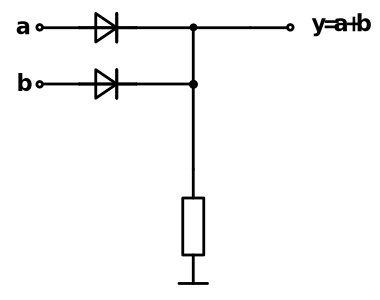
\includegraphics[width=0.3\linewidth]{diodovy_log_OR.pdf}}
        \subfloat[Součinový člen]{\label{ces:fig_D_AND}
          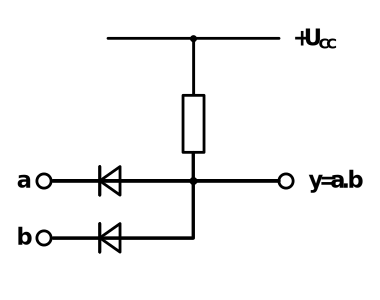
\includegraphics[width=0.3\linewidth]{diodovy_log_AND.pdf}}
        \caption{Diodová logika}
        \label{CES:fig_diodova_logika}
      \end{figure}
   \section{Unipolární digitální obvody}\label{CES:Unipolar_technology} 
  %-------------Přizpůsobení logických obvodů různých napěťových tříd-----------------------------
  % source: AN/Microchip/AN_3V_5V_Digital_Interfacing.pdf
  \newpage
  \section{Přizpůsobení logických obvodů různých napěťových tříd} %Digital Interfacing
    % When interfacing two devices that operate at different voltages, it is imperative to know the
    % output and input thresholds of both devices. Once these values are known, a technique can be
    % selected for interfacing the devices based on the other requirements of your application.
    % Table \ref{CES:tab_threshold} contains the output and input thresholds that will be used
    % throughout this document. When designing an interface, make sure to reference your
    % manufacturers data sheet for the actual threshold levels.
    Vyskytne-li se v číslicovém návrhu potřeba použít logická hradla z odlišných napěťových tříd,
    budeme postaveni před problém jejich vzájemného propojení zachovávající jejich funkčnost. Pro
    správnou volbu vhodného napěťového přizpůsobení logických hradel z různých rodin, je nutné znát
    nejen jejich rozhodovací napětí, ale také následující parametry, které jsou uvedeny v tabulce
    \ref{CES:tab_threshold} \cite[p.~22]{DS41285A}:
    
    \begin{itemize}\addtolength{\itemsep}{-0.5\baselineskip}
      \item maximální úroveň logické '0' na vstupu hradla - $\mathbf{V_{IL_{max}}}$
      \item minimální úroveň logické '1' na vstupu hradla - $\mathbf{V_{IH_{min}}}$
      \item maximální úroveň logické '0' na výstupu hradla - $\mathbf{V_{OL_{max}}}$
      \item minimální úroveň logické '1' na výstupu hradla - $\mathbf{V_{OH_{min}}}$
    \end{itemize}
    
    \begin{table*}
      \centering
      \begin{tabular}{|>{\columncolor{Tan}}l||c|c|c|c|}
        \hline
        \rowcolor{CornflowerBlue}{ }    & {$\mathbf{V_{OH_{min}}}$} & {$\mathbf{V_{OL_{max}}}$} & %
                                          {$\mathbf{V_{IH_{min}}}$} & {$\mathbf{V_{IL_{max}}}$} \\
        \hline
        \hline
        \texttt{5V TTL}                       
                    & 2.4V            & 0.5V       & 2.0V              & 0.8             \\
        \hline
        \texttt{3.3V LVTTL}          
                    & 2.4V            & 0.4V       & 2.0V              & 0.8             \\
        \hline
                    & 4.7V            & 0.5V       & 3.5V              & 1.5V            \\
        \multirow{-2}*{\texttt{5V CMOS}}      
                    & ($V_{CC}$-0.3V) &            & (0.7x$V_{CC}$)    & (0.3x$V_{CC}$)  \\
        \hline
                    
                    & 3.0V            & 0.5V       & 2.3V              & 1.0V            \\
        \multirow{-2}*{\texttt{3.3V LVCMOS}} 
                    & ($V_{CC}$-0.3V) &            & (0.7x$V_{CC}$)    & (0.3x$V_{CC}$)  \\
        \hline 
      \end{tabular}
      \caption{Rozhodovací úrovně napěťových tříd: \texttt{5V TTL}, \texttt{3.3V LVTTL}, 
                                                   \texttt{5V CMOS}, \texttt{3.3V
      LVCMOS}}\label{CES:tab_threshold}
    \end{table*}
    Úroveň logické nuly a jedničky na výstupu určuje konstrukce koncové části digitálního obvodu.
    Nejčastější provedení jsou na obr. \ref{ces:fig_digit_out_common}. Jsou-li různé digitální
    obvody připojeny na společnou sběrnici, může dojít k situaci, kdy některý z výstupních vývodů
    bude buzen vyšším napětím než je napájecí napětí příslušného obvodu. I v tomto případě výstupní
    část digitálního obvodu rozhoduje o výsledném chování. Shrňme základní vlastnosti technologií
    číslicových obvodů uvedených na obr. \ref{ces:fig_digit_out_common}:
    \begin{itemize}
      \item Bipolární koncový stupeň nedovoluje plný rozkmit výstupního signálu. Je-li obvod
            napájen \SI{5}{\volt}, je výstup při úrovni H limitován na $V_{CC}-2\times V_{BE}$(cca
            3.6V). To je hodnota, která na rozhraní \SI{3}{\volt} systému nezpůsobuje příliš velký
            napěťový rozdíl, a tedy proudu, tekoucímu z napájecího zdroje \SI{5}{\volt} systému do
            zdroje \SI{3}{\volt} systému.
      \item Výstupní napětí typické \texttt{CMOS} součástky se prakticky pohybuje v rozsahu
            \texttt{GND} - \texttt{VCC}.
      \item Některé součástky mají výstup typu \emph{open kolektor - OC} resp. \emph{open drain -
            OD}, tj. neexistuje vnitřní obvod, jenž by uvedl výstup do stavu H. K tomu je zapotřebí
            \emph{pull-up} rezistoru, který připojí výstup k napětí, které může být i vyšší než je
            napájecí - \texttt{VCC}. Očividně, tento způsob umožňuje relativně snadné rozhraní, ale
            pro dosažení vyšších rychlostí je nutné volit relativně malý odpor, což zvyšuje
            spotřebu.
      \item U \texttt{NMOS} stupně je podobně jako u bipolárního stupně výstupní napětí logické
            úrovně H omezeno úbytkem na kanálu horní NMOS tranzistoru na $V_{CC} - V_{TH}\simeq
            \SI{3.5}{\volt}$. Obvykle je tedy možné přímé řízení 3V systému.
    \end{itemize}

    \begin{figure}[ht!]
         \centering
         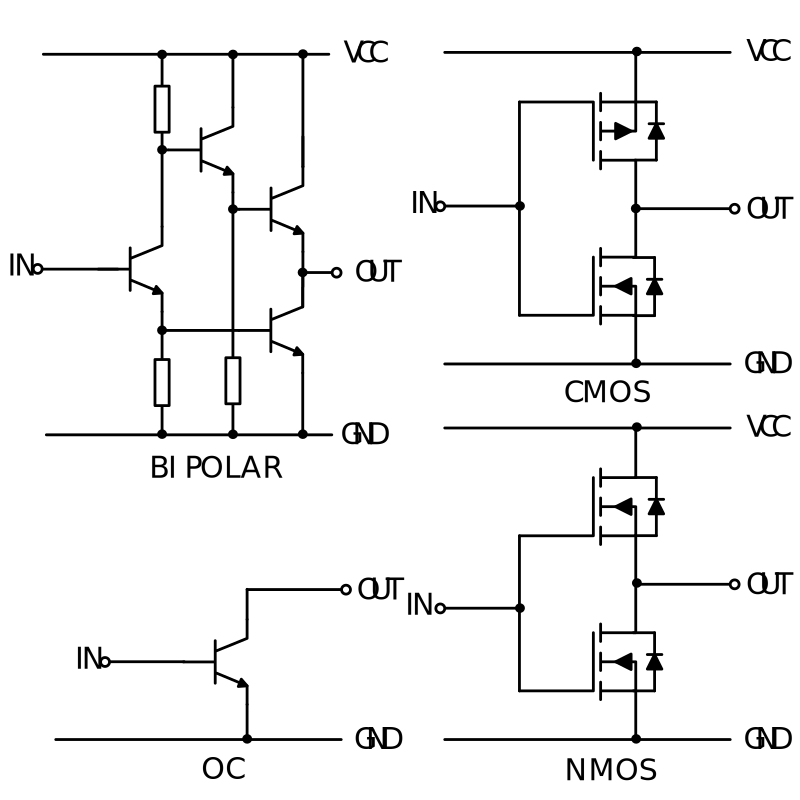
\includegraphics[width=0.7\linewidth]{digit_cir_output_common.pdf}
         \caption[Koncové stupně digitálních obvodů]
                 {Koncové stupně bipolárních, CMOS, NMOS obvodů a obvodů s otevřeným kolektorem 
                  \cite[p.~2]{AN240}}
         \label{ces:fig_digit_out_common}
    \end{figure}   
    
    % --------  Přizpůsobení: 3.3V -> 5V --------------------------- 
    \subsection{3.3V $\rightarrow$ 5V} %3.3V to 5V
      % The simplest and most desired way to connect a 3.3V output to a 5V input is by a direct
      % connection.  This can be done only if the following 2 requirements are met:
      Nejjednodušším a nejvíce žádoucím způsobem je přímé připojení 3.3V výstupu k 5V vstupu, což
      lze provést pouze v případě, že jsou splněny následující požadavky:
        \begin{itemize}\addtolength{\itemsep}{-0.5\baselineskip}
          \item $V_{OH}(3.3V)>V_{IH}(5V)$,
          \item $V_{OL}(3.3V)<V_{IL}(5V)$.
        \end{itemize}
      Hodnoty prahových napětí logické nuly a jedničky v předchozí tabulce \ref{CES:tab_threshold}
      dokládají, že v případě logiky \texttt{3.3V LVCMOS} a \texttt{5V TTL} je možné použít přímého
      připojení. 
      % An example of when this technique can  be used is interfacing a 3.3V LVCMOS output to a 5V
      % TTL input. From the values given in Table 4-1, it can clearly be  seen that both of these
      % requirements are met.

      % 3.3V LVCMOS VOH of 3.0 volts is greater than 5V TTL VIH of 2.0 volts and 3.3V LVCMOS VOL
      % of 0.5 volts is less than 5V TTL VIL of 0.8 volts.

      Pokud oba tyto požadavky nejsou splněny, je třeba použít na rozhraní obou logik
      přizpůsobovací obvody, popsané v následujících textu. 
      % When both of these requirements are  not met, some additional circuitry will be needed to
      % interface the two parts.

      \subsubsection{MOSFET Translator}
        \begin{figure}[ht!]
           \centering
           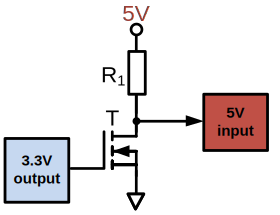
\includegraphics[scale=0.5]{level_shifting_MOSFET.pdf}
           \caption{3.3V $\rightarrow$ 5V: N-MOSFET}
           \label{CES:fig_shifting_MOSFET}
           \vspace*{-1\baselineskip}
        \end{figure}
        % In order to drive any 5V input that has a higher VIH than the VOH of a 3.3V CMOS part,
        % some additional circuitry is needed. A low-cost two component solution is shown in Figure
        % 6-1. When selecting the value for R1, there are two parameters that need to be considered;
        % the switching speed of the input and the current consumption through R1.
        Levné a jednoduché řešení problému vzájem\-ného přizpůsobení logických obvodů odliš\-ných
        napěťových tříd, pro které platí $V_{OH}(3.3V)<V_{IH}(5V)$ nabízí použití MOSFETu s
        prahovým napětím $$V_{GS_{th_{max}}}<V_{OH_{min}}.$$ Při výběru hodnoty $R_1$ je třeba vzít
        v úvahu:
        \begin{itemize}\addtolength{\itemsep}{-0.5\baselineskip}
          \item spínací rychlost vstupu,
          \item zvýšení spotřeby díky proudu přes rezistor $R_1$.
        \end{itemize}

        Při změně logické úrovně $'0'\rightarrow'1'$ na vstupu 5V logiky je nutné počítat se
        zpožděním, které je dáno časovou konstantu RC článku, tvořeného rezistorem $R_1$ a celkovou
        kapacitou na vstupu hradla. Důsledkem je tedy určitá minimální spínací perioda: 
        % When switching the input from a ‘0’ to a ‘1’, you will have to account for the time the
        % input takes to rise because of the RC time constant formed by R1, and the input
        % capacitance of the 5V input plus any stray capacitance on the board. The speed at which
        % you can switch the input is given by the following:
        $$T_{SW_{min}} = 3 \cdot R_1 \cdot C_{IN},$$ která je vyšší, čím nižší spotřeby se návrhář
        snaží dosáhnout ($R_1\uparrow$). Zpoždění při spínání $'1'\rightarrow'0'$ má příznivější
        hodnotu, neboť $R_{dsON}\ll R_1$.

        % Since the input and stray capacitance of the board are fixed, the only way to speed up
        % the switching of the input is to lower the resistance of R1. The trade-off of lowering
        % the resistance of R1 to get faster switching times is the increase in current draw when
        % the 5V input remains low. The switching to a ‘0’ will typically be much faster than
        % switching to a ‘1’ because the ON resistance of the N-channel MOSFET will be much smaller
        % than R1. Also, when selecting the N-channel FET, select a FET that has a lower VGS
        % threshold voltage than the VOH of 3.3V output.

      \subsubsection{Diodový Offset}
        Hodnoty vstupního prahového napětí \texttt{5V CMOS} a výstupní prahová napětí pro
        \texttt{3.3V LVTTL} a \texttt{LVCMOS} jsou uvedeny v tabulce \ref{CES:tab_diode_offset}
        % The inputs voltage thresholds for 5V CMOS and the output drive voltage for 3.3V LVTTL and
        % LVCMOS are listed in Table 7-1.
        \begin{table*}[t]
          \centering
          \begin{tabular}{|>{\columncolor{Tan}}l|c|c|c|}
            \hline
              \cellcolor{CornflowerBlue}                                   
                & \cellcolor{CornflowerBlue}\textbf{5V CMOS}       & 
              \cellcolor{CornflowerBlue} \textbf{3.3V LVTTL}               
                & \cellcolor{CornflowerBlue} \textbf{3.3V LVCMOS}  \\
              \multirow{-2}*{\cellcolor{CornflowerBlue}\texttt{Threshold}} 
                & \cellcolor{CornflowerBlue} IN 
                & \cellcolor{CornflowerBlue} OUT
                & \cellcolor{CornflowerBlue} OUT                   \\
            \hline\hline
               \texttt{High}                                               
                & $>3.5V$  & $>2.4V$ & $>3.0V$                     \\
               \texttt{Low}                                         
                & $<1.5V$  & $<0.4V$ & $<0.5V$                     \\
            \hline          
          \end{tabular}
          \caption{Přehled vstupní a výstupních prahový napětí různých logik, chceme-li ke vstupu
          \texttt{5V CMOS} připojit \texttt{3.3V LVTTL} nebo \texttt{3.3V LVCMOS.\cite{AN240}}}
          \label{CES:tab_diode_offset}
        \end{table*}

        \begin{figure}[ht!]
            \centering
            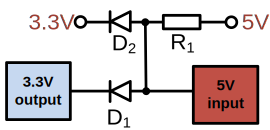
\includegraphics[scale=0.5]{level_shifting_diode_offset.pdf}
            \caption{3.3V $\rightarrow$ 5V: Diodový offset}
            \label{CES:fig_shifting_D_offset}
        \end{figure}

        Všimněme si, že obě prahová napětí vstupu \texttt{5V CMOS} logiky jsou o volt vyšší než u
        výstupu 3.3V logiky. Zapotřebí je tedy obvod, který zvyšuje vysokou a nízkou úroveň
        prahového napětí.
        % Note that both the high and low threshold input voltages for the 5V CMOS inputs are about
        % a volt higher than the 3.3V outputs. So, even if the output from the 3.3V system could be
        % offset, there would be little or no margin for noise or component tolerance. What is
        % needed is a circuit that offsets the outputs and increases the difference between the
        % high and low output voltages.

        Pokud bychom vytvořili posunutí o alespoň o 0.7V pro obě úrovně prahového napětí, dosáhli
        bychom vzájemného přizpůsobení. Obvod na obr. \ref{CES:fig_shifting_D_offset}, posuneme
        hodnotu nízké úrovně výstupního prahového napětí o úbytek v propustném směru diody $D_1$
        (typicky 0.7V), na 1.1V až 1.2V. Úroveň vysokého prahového napětí se nastavuje pomocí
        pull-up rezistoru a diody $D_2$ vázané na 3.3V napájení. Výstupní napětí je tedy také
        posunuto přibližně 0,7V nad 3,3V napájení, tj. na 4,0 až 4.1V, což je vysoko nad 3,5V
        prahem vstupu 5V CMOS logiky.

        % When output voltage specifications are determined, it is done assuming that the output is
        % driving a load between the output and ground for the high output, and a load between 3.3V
        % and the output for the low output. If the load for the high threshold is actually between
        % the output and 3.3V, then the output voltage is actually much higher as the load resistor
        % is the mechanism that is pulling the output up, instead of the output transistor.

        % If we create a diode offset circuit (see Figure 7-1), the output low voltage is increased
        % by the forward voltage of the diode D1, typically 0.7V, creating a low voltage at the 5V
        % CMOS input of 1.1V to 1.2V. This is well within the low threshold input voltage for the
        % 5V CMOS input. The output high voltage is set by the pull-up resistor and diode D2, tied
        % to the 3.3V supply. This puts the output high voltage at approximately 0.7V above the
        % 3.3V supply, or 4.0 to 4.1V, which is well above the 3.5V threshold for the 5V CMOS input
        \vskip2mm
        \begin{note}
          Aby obvod fungoval správně, musí být pull-up rezistor podstatně menší než vstupní odpor
          5V CMOS logiky, aby se zabránilo snížení výstupního napětí díky efektu vstupního
          odporového děliče a také musí být dostatečně velký, aby proud tekoucí do 3.3V napájení a
          výstupu hradla byl v mezích specifikace. 
          % For the circuit to work properly, the pull-up resistor must be significantly smaller
          % than the input resistance of the 5V CMOS input, to prevent a reduction in the output
          % voltage due to a resistor divider effect at the input. The pull-up resistor must also
          % be large enough to keep the output current loading on the 3.3V output within the
          % specification of the device.
        \end{note}

      \subsubsection{Komparátor}
        Základní funkce komparátoru je následující:        
        % The basic operation of the comparator is as follows:
        \begin{itemize}\addtolength{\itemsep}{-0.5\baselineskip}
          \item napětí na invertující (-) vstupu je větší než na neinvertujícím vstupu (+), výstup
                komparátoru se nastaví do nízké úrovně, 
                % When the voltage at the inverting (-) input is greater than that at the
                % non-inverting (+) input, the output of the comparator swings to Vss.
          \item je-li napětí na neinvertujícím vstupu (+) větší než na invertujícím vstupu (-),
                výstup komparátoru se nastaví do vysoké úrovně. %When the voltage at the
                % non-inverting (+) input is greater than that at the non-inverting (-)
                % input, the output of the comparator is in a high state.
        \end{itemize}

        \begin{figure}[ht!]
            \centering\vspace*{+1\baselineskip}
            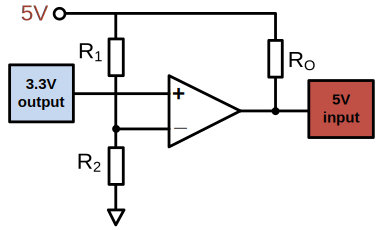
\includegraphics[scale=0.5]{level_shifting_COMP.pdf}
            \caption{3.3V $\rightarrow$ 5V: Komparátor; $R_1 = 1,8 k\Omega, R_2 = 1 k\Omega$}
            \label{CES:fig_shifting_COMP}           
        \end{figure}

        \textbf{Výpočet hodnoty odporu $R_1$ a $R_2$:}\newline
          Poměr R1 a R2 je závislý na napětí logické nuly a jedničky na výstupu hradla 3.3V logiky.
          Invertující vstup by měl být nastaven do poloviny mezi prahovými hladinami $V_{OL}$ a
          $V_{OH}$. Pro \texttt{LVCMOS} je toto napětí rovno $$1.75V = \frac{3V+0.5V}{2}.$$
          Budeme-li volit velikost $R_2$, pak hodnotu odporu $R_1$ snadno dopočítáme dle
          následující rovnice: $$R_1=R_2\left(\frac{5V}{1.75V}-1\right).$$ 
          % The ratio of R1  and R2  depends on the logic levels of the input signal. The inverting
          % input should be set to a voltage halfway between VOL and VOH for the 3.3V output. For
          % an LVCMOS output, this voltage is: $$1.75V = \frac{3V+0.5V}{2}.$$ Given that R1 and R2
          % are related by the logic levels:
          % $$R_1=R_2\left(\frac{5V}{1.75V}-1\right)$$ assuming a value of 1K for R2, R1 is 1.8K.

    % --------  Přizpůsobení: 5V -> 3.3V ---------------------------
    \subsection{5V $\rightarrow$ 3.3V} %5V to 3.3V
      \subsubsection{Přímé propojení}
        \begin{figure}[ht!]
            \centering
            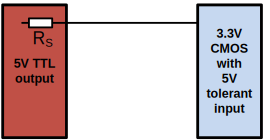
\includegraphics[scale=0.6]{direct_connect.pdf}
            \caption{5V $\rightarrow$ 3,3V: Přímé propojení}
            \label{CES:fig_dir_connect}
        \end{figure}

        Hradla napěťové třídy 5V mají výstupy s typickými prahovými hodnotami $V_{OH} = 4,7 V$,
        $V_{OL} = 0,4 V$ zatímco hradla 3.3V LVCMOS mají vstupy s prahovými hodnotami $V_{IH} =
        0,7\times V_{DD} $, $V_{IL} = 0,2\times V_{DD}$. Je-li tedy na 5V výstupu logická nula,
        bude také správně interpretována 3V vstupem, neboť platí $V_{OL} = 0,4 < V_{IL} = 0,8$. Ani
        v případě logické jedničky nevzniká žádný konflikt, neboť $V_{OH} = 4,7 > V_{IH} = 2,1$.
        Pokud je tedy 3V vstup 5V tolerantní, je možné přímé propojení, v opačném případě je třeba
        použít některou z následujících technik.
        % 5V outputs have a typical VOH of 4.7 volts and a VOL of 0.4 volts and a 3.3V LVCMOS input
        % will have a typical VIH of 0.7 x VDD and a VIL of 0.2 x VDD. When the 5V output is
        % driving low, there are no problems because the 0.4 volt output is less than in the input
        % threshold of 0.8 volts. When the 5V output is high, the VOH of 4.7 volts is greater than
        % 2.1 volt VIH, therefore, we can directly connect the 2 pins with no conflicts if the 3.3V
        % CMOS input is 5 volt tolerant. If the 3.3V CMOS input is not 5 volt tolerant, then there
        % will be an issue because the maximum volt specification of the input will be exceeded.

      \subsubsection{Diodový omezovač} %Diode Clamp
        Některé digitální obvody mají své vstupy chráněny vnitřními omezovacími diodami tzv.
        \texttt{diode clamp} (obr. \ref{CES:fig_int_clamp_D}). Proteče-li těmito diodami větší proud
        než udávají katalogové hodnoty, může dojít k poškození vstupu, nebo v lepším případě k
        efektu \texttt{latching-up}. Typický 5V výstup má kolem $10 \Omega$, proto chceme-li využít
        těchto diod, musíme přidat sériový odpor, jenž limituje velikost propustného proudu.
        Nepříjemným důsledkem je ovšem vzniklý RC článek se vstupní kapacitou hradla $C_L$, který
        snižuje rychlost. Není-li vstup takto chráněn je možné jej doplnit externí diodou dle obr.
        \ref{CES:fig_ext_clamp_D}.
        % Many manufacturers protect their I/O pins from exceeding the maximum allowable voltage
        % specification by using clamping diodes. These clamping diodes keep the pin from going
        % more than a diode drop below Vss and a diode drop above VDD. To use the clamping diode to
        % protect the input, you still need to look at the current through the clamping diode. The
        % current through the clamp diodes should be kept small (in the micro amp range). If the
        % current through the clamping diodes gets too large, then you risk the part latching up.
        % Since the source resistance of a 5V output is typically around 10 ohms, an additional
        % series resistor is still needed to limit the current through the clamping diode as shown
        % Figure 10-1. The consequence of using the series resistor is it will reduce the speed at
        % which we can switch the input because the RC time constant formed the capacitance of the
        % pin (CL).
       \begin{figure}[ht!]
         \centering
         \begin{tabular}{c}
           \subfloat[Vnitřními omezovací diody]{\label{CES:fig_int_clamp_D}
             \includegraphics[width=0.3\textwidth]{CES_clamp_diodes_input.png}}        \\
           \subfloat[Externí omezovací dioda]{\label{CES:fig_ext_clamp_D}     
             \includegraphics[width=0.3\textwidth]{CES_ext_clamp_diodes_input.png}}
         \end{tabular}  
         \caption{5V $\rightarrow$ 3,3V: Použití omezovacích diod pro ochranu vstupu integrovaného
                  obvodu}
         \label{CES:fig_clamp_diodes}
       \end{figure} 
        % One problem with using a diode clamp is that it injects current onto the 3.3V power
        % supply. In designs with a high current 5V outputs, and lightly loaded 3.3V power supply
        % rails, this injected current can float the 3.3V supply voltage above 3.3V. To prevent
        % this problem, a transistor can be substituted which routes the excess output drive
        % current to ground instead of the 3.3V supply.
          
        Dalším problémem je proud, injektovaný z 5V výstupu skrz omezovovací diodu do 3.3V
        napájení. Tento proud může způsobit zvýšení napájecího napětí 3.3V obvodů, což může vést k
        jejich zničení. Proto lze s výhodou použít PNP tranzistor zapojený dle obr.
        \ref{CES:fig_bjt_clamp}.
        
        \begin{figure}[ht!]
          \centering
          \includegraphics[scale=0.5]{CES_ext_clamp_bjt_input.png}
          \caption{5V $\rightarrow$ 3,3V: Active clamp - Přechod báze-emitor funguje jako omezovací
                   dioda, ovšem s tím rozdílem, že jen malé procento celkového proudu z 5V výstupu
                   teče do 3.3V napájení. Převážná část teče kolektorem do země. Poměr bázového a
                   kolektorového proudu je určen proudovým zesílením tranzistoru, které je typicky
                  10 až 400}
          \label{CES:fig_bjt_clamp}
        \end{figure}              
       
      \subsubsection{Napěťový dělič} %Resistor divider
        A simple resistor divider can be used to reduce the output of a 5V device to levels
        appropriate for a 3.3V device input. An equivalent circuit of this interface is shown in
        Figure \ref{CES:fig_res_divider}.
        \begin{figure}[ht!]
          \centering
          \includegraphics[scale=0.4]{CES_ext_res_divider.png}
          \caption{5V $\rightarrow$ 3,3V: napěťový děliš}
          \label{CES:fig_res_divider}
        \end{figure}
        Typically, the source resistance, $R_S$, is very small (less than 10 ohms) so its affect on
        $R_1$ will be negligible provided that $R_1$ is chosen to be much larger than $R_S$. At the
        receive end, the load resistance, $R_L$, is very large (greater than 500 k ohms) so its
        affect on $R_2$ will be negligible provided that $R_2$ is chosen to be much less than
        $R_L$.
        
        There is a trade-off between power dissipation and transition times. To keep the power
        requirements of the interface circuit at a minimum, the series resistance of $R_1$ and
        $R_2$ should be as large as possible. However, the load capacitance, which is the
        combination of the stray capacitance, $C_S$, and the 3.3V device input capacitance, $C_L$,
        can adversely affect the rise and fall times of the input signal. Rise and fall times can
        be unacceptably long if $R_1$ and $R_2$ are too large.
        
        Neglecting the affects of $R_S$ and $R_L$, the formula for determining the values for $R_1$
        and $R_2$ is given by Equation \ref{CES:eq_res_divider}.
        \begin{align}\label{CES:eq_res_divider}
          \frac{V_S}{R_1+R_2} &= \frac{V_L}{R_2}           \nonumber \\
                          R_1 &= \frac{(V_S-V_L)}{V_L}R_2  \nonumber \\
                          R_1 &= 0,515\cdot R_2
        \end{align}      
        The formula for determining the rise and fall times is given in Equation
        \ref{CES:eq_res_divider_time}. For circuit analysis, the Thevenin equivalent is used to
        determine the applied voltage, $V_A$, and the series resistance, $R$.
        The Thevenin equivalent is defined as the open circuit voltage divided by the short circuit
        current. The Thevenin equivalent, $R$, is determined to be $0.66\cdot R_1$ and the Thevenin
        equivalent, $V_A$, is determined to be $0.66\cdot V_S$ for the circuit shown in  Figure
        \ref{CES:fig_res_divider} according to the limitations imposed by Equation
        \ref{CES:eq_res_divider_time}.
        \begin{equation}\label{CES:eq_res_divider_time}
          t = - R\cdot C \cdot \ln\left(\frac{V_F-V_A}{V_I-V_A}\right)
        \end{equation}  
        kde $t$ = Rise or Fall time, $R = 0.66\cdot R_1$, $C = C_S+C_L$, $V_I$ = Initial voltage on
        $C$ ($V_L$), $V_F$ = Final voltage on $C$ ($V_L$), $V_A$ = Applied voltage ($0.66\cdot V_S$). 
        \begin{example} As an example, suppose the following conditions exist:
          \begin{itemize}\addtolength{\itemsep}{-0.5\baselineskip}
            \item Stray capacitance = 30 pF,
            \item Load capacitance = 5 pF,
            \item Maximum rise time from 0.3V to 3V ≤ 1 μS
            \item Applied source voltage Vs = 5V
          \end{itemize}
          Solve Equation \ref{CES:eq_res_divider_time} for $R$:  
          \begin{equation*}
            R = - \dfrac{t}{C\cdot\ln\dfrac{V_F-V_A}{V_I-V_A}}
          \end{equation*}   
          Substitute values:
          \begin{equation*}
            R = - \dfrac{10\cdot10^{-7}}{35\cdot10^{-12}\cdot
                  \ln\dfrac{3-0.66\cdot5}{0.3-0.66\cdot5}}
          \end{equation*}               
          Thevenin equivalent maximum R: $$R = 12408$$
          Solve for maximum $R_1$ and $R_2$:
          \begin{alignat}{3}
            & R_1 &&= 0.66\cdot R  \qquad &&R_2 = \frac{R_1}{0.515}  \\
            & R_1 &&= 8190         \qquad &&R_2 = 15902 
          \end{alignat}          
        \end{example} 
                   
      \subsubsection{Level translator} %Level translator
        While level translation can be done discretely, it is often preferred to use an integrated
        solution. Level translators are available in a wide range of capabilities. There are
        unidirectional and bidirectional configurations, different voltage translations and
        different speeds, all giving the user the ability to select the best solution. 
        \begin{figure}[ht!]
          \centering
          \begin{tabular}{c}
            \subfloat[SPI sběrnice]{\label{CES:fig_level_translator1}
              \includegraphics[width=0.9\linewidth]{CES_ext_level_translator1.png}}           \\
            \subfloat[I2C sběrnice]{\label{CES:fig_level_translator2}
              \includegraphics[width=0.9\linewidth]{CES_ext_level_translator2.png}}
          \end{tabular}  
          \caption{5V $\rightarrow$ 3,3V: Board-level communication between devices (e.g., MCU to
                   peripheral) is most often done by either SPI or I2C. For SPI, it may be
                   appropriate to use a unidirectional level translator and for I2C, it is necessary
                   to use a bidirectional solution.}
          \label{CES:fig_level_translator}
        \end{figure}           
      
} % tikzset
%---------------------------------------------------------------------------------------------------
\printbibliography[title={Seznam literatury}, heading=subbibliography]
\addcontentsline{toc}{section}{Seznam literatury} 
%======================= Kapitola03: Základy mikroprocesorové techniky =============================
  \input{../src/CES/chap/Basic_MCU_Arch.tex} 
%======================= Kapitola04: Historie mikroprocesorové techniky ============================
  % !TeX spellcheck = cs_CZ
%{\tikzset{external/prefix={tikz/CES/}}
% \tikzset{external/figure name/.add={ch02_}{}}
%---------------------------------------------------------------------------------------------------
% file Basic_MCU_Arch.tex
%---------------------------------------------------------------------------------------------------
\lstset{ %
  language={[x86masm]Assembler},         % choose the language of the code
  inputencoding=latin1,
  extendedchars=true,
  showspaces=false,                      % show spaces everywhere adding particluar undescores, it  
                                         % overrides 
                                         % “showstringspaces”
  showstringspaces=false,                % underline spaces within strings only
  basicstyle=\footnotesize\ttfamily,     % the size of the fonts that are used for the code
%  backgroundcolor=\color{White},        % choose the background color. You must add  
                                         % \usepackage{color}
  breaklines=true,                       % sets automatic line breaking
  breakatwhitespace=true,                % sets if automatic breaks should only happen at whitespace
  showspaces=false,                      % show spaces adding particular underscores
  showstringspaces=true,                 % underline spaces within strings
  showtabs=true,                         % show tabs within strings adding particular underscores
  frame=none,                            % adds a frame around the code - none, single
  tabsize=2,                             % sets default tabsize to 2 spaces
  captionpos=b,                          % sets the caption-position to bottom
  numbers=left,                          % where to put the line-numbers -none, left, right
  numberstyle=\tiny\color{lstnumcolor},  % the size of the fonts that are used for the line-numbers
  numbersep=5pt,                         % how far te line-number are from the code
  stepnumber=1,                          % the step between two line-numbers. If it's 1 each line
                                         % will be numbered
  xleftmargin=3em,                       % adjust left margin
  commentstyle=\color{help}\textit,      % comment style
  keywordstyle=\color{keyword}\textbf,   % keyword style
  morekeywords={ADDC, ASHR, SUBB,CLR,    % if you want to add more keywords to the set
    MAC,  MULS, DIVS, BSET, BCLR, BCPL, 
    BAND, BOR,  BXOR, BCMP, TRL,  EX,  BMOV,
    JCC,  BCC,  DJNZ, RETI, JSR,  CSP, LDR},
  literate= %
    {á}{{\'a}}1  {é}{{\'e}}1     {í}{{\'i}}1   {ó}{{\'o}}1   {ú}{{\'u}}1
    {Á}{{\'A}}1  {É}{{\'E}}1     {Í}{{\'I}}1   {Ó}{{\'O}}1   {Ú}{{\'U}}1
    {à}{{\`a}}1  {è}{{\`e}}1     {ì}{{\`i}}1   {ò}{{\`o}}1   {ù}{{\`u}}1
    {À}{{\`A}}1  {È}{{\'E}}1     {Ì}{{\`I}}1   {Ò}{{\`O}}1   {Ù}{{\`U}}1
    {ä}{{\"a}}1  {ë}{{\"e}}1     {ï}{{\"i}}1   {ö}{{\"o}}1   {ü}{{\"u}}1
    {Ä}{{\"A}}1  {Ë}{{\"E}}1     {Ï}{{\"I}}1   {Ö}{{\"O}}1   {Ü}{{\"U}}1
    {â}{{\^a}}1  {ê}{{\^e}}1     {î}{{\^i}}1   {ô}{{\^o}}1   {û}{{\^u}}1
    {Â}{{\^A}}1  {Ê}{{\^E}}1     {Î}{{\^I}}1   {Ô}{{\^O}}1   {Û}{{\^U}}1
    {œ}{{\oe}}1  {Œ}{{\OE}}1     {æ}{{\ae}}1   {Æ}{{\AE}}1   {ß}{{\ss}}1
    {ç}{{\c c}}1 {Ç}{{\c C}}1    {ø}{{\o}}1    {å}{{\r a}}1  {Å}{{\r A}}1
    {€}{{\EUR}}1 {£}{{\pounds}}1 {ř}{{\v{r}}}1 {ž}{{\v{z}}}1 {č}{{\v{c}}}1
    {ě}{{\v{e}}}1
}
%================== Kapitola: Základy mikroprocesorové techniky====================================
%\setchaptertoc
\chapter{Historie mikroprocesorové techniky}
\minitoc
    \subsection{Vývoj mikroprogramových řadičů: od mainframu EDSAC k moderním 
                 mikroprocesorům}\hypertarget{MIT:sec_003}
      Na princip funkce mikrořadiče řízeného pomocí mikroprogramů, jenž byl popsaný v kapitole 
      \ref{ces:IchapIVsecIIssecI}, se můžeme dívat jako na zobecnění idey programování počítačů 
      pomocí instrukcí uložených v operační paměti. V samých počátcích vývoje výpočetní techniky, 
      konkrétně u takzvané nulté generace (zhruba do roku 1947) a první generace (cca roky 1946 až 
      1958) počítačů, se totiž algoritmy nevyjadřovaly pomocí instrukcí tvořících ucelené programy, 
      které by byly uloženy do paměti. Namísto toho byl algoritmus „zadrátován“ (obr. 
      \ref{MIT:fig_eniac}) takovým způsobem, že se pomocí vodičů umístěných většinou na spínacích 
      panelech vzájemně propojovaly jednotlivé moduly počítače – sčítačky, pracovní registry, 
      řadiče paměti, vstupní prvky atd. Navíc se u některých specializovaných počítačů používaných 
      za druhé světové války pro luštění šifer nedal algoritmus vůbec měnit – počítač stále 
      prováděl stejné výpočty, ovšem s různými daty. Tato konstrukce počítačů odpovídala dobové 
      technologii, které se používala především v telefonních ústřednách s ručním přepojováním 
      hovorů, semaforech nebo například pro ovládání výtahů.
      
      \begin{figure}[ht!]   %\ref{MIT:fig_eniac}
        \centering
        \includegraphics[width=0.9\linewidth]{eniac.jpg}
        \caption{Způsob programování elektronického počítače \Eniac (\emph{Electronic Numerical 
                 Integrator And Computer}) pomocí vzájemného propojování jednotlivých modulů 
                 přepojováním kabelů mezi jednotlivými funkčními moduly. Kredit: Columbia 
                 university}
        \label{MIT:fig_eniac}
      \end{figure}
      
      \subsubsection{Von Neumannova architektura programovatelného počítače}
        Ovšem již v polovině čtyřicátých let minulého století přišel \wikiNeumann s převratnou 
        myšlenkou – libovolný algoritmus nemusí být přímo „zadrátován“ v počítači, ale může být 
        zapsán ve formě programu složeného ze sekvence instrukcí, které mohou být uloženy v paměti 
        počítače naprosto stejným způsobem, jako zpracovávaná data; viz též dnes již klasické von 
        Neumannovo dílo \wikiEDVAC vydané v roce 1945. Právě díky této myšlence vznikly první 
        skutečné procesory s instrukčními sadami, děrné štítky se začaly používat mj. i pro uložení 
        programů a navíc se otevřela cesta k dalšímu zobecnění: programy začaly být asi o deset let 
        později vytvářeny ve vyšších programovacích jazycích, přičemž překlad prováděl jiný program 
        (algoritmus) nazývaný překladač (dnes bereme překladače jako zcela běžnou věc, ale idea, že 
        překladač je sám o sobě taktéž algoritmem, byla v době její implementace chápána jako malá 
        revoluce). Toto dvojí zobecnění práce univerzálního programovatelného počítače nebylo 
        dodnes překonáno a je na něm založena i moderní výpočetní technika a informatika.
        
        Architektura počítačů navržená John von Neumannem byla založena na \emph{centrální 
        procesorové jednotce} rozdělené na \emph{aritme\-ticko-logickou jednotku} a 
        \emph{řadič}, 
        který na základě instrukcí čtených z operační paměti řídil všechny další moduly počítače 
        (vstupně-výstupní zařízení, aritmeticko-logickou jednotku, operační paměť). Nikde ovšem 
        nebylo přesně specifikováno, jakým způsobem má být řadič, jakožto „mozek“ počítače, 
        implementován. V prvních mainframech založených na myšlence Johna von Neumanna se tedy 
        uplatňovaly obvodové řadiče. Tyto řadiče byly dostatečně rychlé a nevyžadovaly ke své 
        činnosti prakticky žádné paměťové prvky (většinou jen čítač či posuvný registr), ovšem 
        přinášely i některé nevýhody. Jednou z poměrně závažných nevýhod byla velká složitost 
        obvodového řadiče v případě, že se používala komplexnější instrukční sada (\texttt{CISC}). 
        Poněkud paradoxně se právě složité instrukční sady začaly v padesátých letech minulého 
        století stále více používat, zejména na mainframech druhé generace. A právě tehdy se začala 
        prakticky realizovat myšlenka \emph{mikroprogramování}.
      
      \subsubsection{EDSAC – první počítač se skutečným mikroprogramovým řadičem}
        Myšlenka mikroprogramování vznikla již v roce 1951, kdy ji ve svých článcích představil sir 
        \wikiEWilkes (titul sir získal Wilkes právě za svoji dlouholetou práci v oboru 
        \texttt{IT}). Idea mikroprogramování spočívala v zobecnění konstrukce centrální procesorové 
        jednotky (\texttt{CPU}) takovým způsobem, že strojové instrukce byly rozkládány na sekvenci 
        řídicích signálů pomocí mikroprogramu uloženého v paměti typu \texttt{ROM} s velmi rychlou 
        dobou přístupu. Vzhledem ke stavu technologie v roce 1951 samozřejmě V. Wilkes nemohl 
        použít klasický čip s \texttt{ROM}, v němž jsou bity trvale zaznamenány s použitím 
        poslední, zákazníkem definované masky při výrobě čipu. Namísto toho Wilkes navrhoval použít 
        matici navzájem kolmých vodičů, v níž by byla bitová jednička „zaznamenána“ pomocí diody 
        spojující jeden vodorovný a jeden svislý vodič (vodivou kovovou spojku nelze použít, 
        protože by se do matice nepřímo zapsaly i falešné jedničky).
        
        \begin{figure}[ht!]   %\ref{MIT:fig_edsac}
          \centering
          \includegraphics[width=0.95\linewidth]{EDSAC.jpg}
          \caption{\wikiEDSAC (Electronic Delay Storage Automatic Calculator) byl britský počítač z 
                   poloviny 20. století. Tento počítač, inspirovaný John Von Neumannovým dokumentem 
                   First Draft of a Report on the EDVAC, sestavil Maurice Wilkers a jeho tým na 
                   Univerzitě v Cambridgi v Anglii. EDSAC byl první v praxi využitý počítač 
                   pracující s uloženým programem. Kredit: Wikipedia, Root.cz}
          \label{MIT:fig_edsac}
        \end{figure}
        
        Na zpočátku pouze teoretickou práci M. V. Wilkese o několik let později navázali William 
        Renwick a \wikiWheeler, kteří v roce 1957 sestrojili první skutečný počítač založený na 
        mikroprogramovém procesoru. Vzhledem k tomu, že diodová matice navržená Wilkesem by byla 
        příliš rozměrná pro počítač s velkou instrukční sadou (diodami jsou zde samozřejmě myšleny 
        diskrétní elektronické součástky, i když se v roce 1957 již pomalu schylovalo k výrobě 
        prvních prototypů integrovaných obvodů), použili W. Renwick a D. Wheeler namísto diod 
        feritovou paměť, což bylo ve svém důsledku velmi zajímavé, protože se obsah této paměti dal 
        přeprogramovat a tím pádem bylo možné i měnit instrukční sadu počítače. První prototyp 
        tohoto stroje byl nazván \texttt{EDSAC 1½} a používal pro uložení mikroinstrukcí feritovou 
        paměť s maticí o velmi malých rozměrech 6×8 feritových jader – tento počítač ovšem 
        neobsahoval celou instrukční sadu. Finální podoba počítače z roku 1958, jež nesla název 
        \texttt{EDSAC 2}, měla již paměťovou matici o rozměrech 32×32 feritových jader, což již 
        umožnilo implementaci plnohodnotné instrukční sady za použití mikrokódů.
    
%} % tikzset
%---------------------------------------------------------------------------------------------------
\printbibliography[title={Seznam literatury}, heading=subbibliography]
\addcontentsline{toc}{section}{Seznam literatury} 
}  % DEBUG was off

\setpartpreamble[u]{
\begin{center}
  \vspace{1cm}
  \Huge \uppercase{\textbf{Zabudované (embedded)}} \\
  \Huge \uppercase{\textbf{systémy}} \\
  \vspace{2cm}
  \includegraphics[width=0.8\linewidth]{CES.png}
\end{center}
}

\part{CES II}\label{part:CESII}
\parttoc

\ifthenelse{ \equal{\DebugMode}{true} }{
% Debug mode ON
  % !TeX spellcheck = cs_CZ
{\tikzset{external/prefix={tikz/CES/}}
 \tikzset{external/figure name/.add={ch05_}{}}
%---------------------------------------------------------------------------------------------------
% file ANSI_C_MCU.tex
%---------------------------------------------------------------------------------------------------
%============================= Kapitola: Stručný úvod===============================================
\lstset{ %
  language=C,                            % choose the language of the code
  basicstyle=\footnotesize\ttfamily,     % the size of the fonts that are used for the code
  backgroundcolor=\color{White},         % choose the background color. 
  commentstyle=\color{help}\textit,
  keywordstyle=\color{blue}\textbf,
  breaklines=true,                       % sets automatic line breaking
  breakatwhitespace=true,                % sets if automatic breaks should only happen at whitespace
  showspaces=false,                      % show spaces adding particular underscores
  showstringspaces=true,                 % underline spaces within strings
  showtabs=true,                         % show tabs within strings adding particular underscores
  frame=none,	                           % adds a frame around the code - none, single
  tabsize=8,                             % sets default tabsize to 8 spaces
  captionpos=b,                          % sets the caption-position to bottom
  numbers=left,                          % where to put the line-numbers -none, left, right
  numberstyle=\footnotesize,             % the size of the fonts that are used for the line-numbers
  stepnumber=1,                          % the step between two line-numbers. If it's 1 each line
  % will be numbered
  xleftmargin=3em,                       % adjust left margin
}

\chapter{ANSI-C pro mikrokontroléry}
\minitoc

  %============= Podkapitola: Preprocesor jazyka C =================================================
  \section{Preprocesor jazyka C}
    Preprocesor interpretuje jednoduché direktivy pro vložení zdrojového kódu z jiného souboru 
    (\lstinline[basicstyle=\ttfamily]!#include!), definice maker 
    (\lstinline[basicstyle=\ttfamily]!#define!) a podmíněné vložení kódu 
    (\lstinline[basicstyle=\ttfamily]!#if!). \texttt{C} preprocesor přijímá tyto direktivy:
    
    \begin{table}[ht!]
      \centering
      \begin{tabular}{c c c c}
        \hline
        \lstinline[basicstyle=\ttfamily]!#define!  & \lstinline[basicstyle=\ttfamily]!#elif! & 
        \lstinline[basicstyle=\ttfamily]!#else!    & \lstinline[basicstyle=\ttfamily]!#endif! \\
        \lstinline[basicstyle=\ttfamily]!#error!   & \lstinline[basicstyle=\ttfamily]!#if! & 
        \lstinline[basicstyle=\ttfamily]!#ifdef!   & \lstinline[basicstyle=\ttfamily]!#ifndef! \\
        \lstinline[basicstyle=\ttfamily]!#include! & \lstinline[basicstyle=\ttfamily]!#line! & 
        \lstinline[basicstyle=\ttfamily]!#pragma!  & \lstinline[basicstyle=\ttfamily]!#undef! \\
        \hline            
      \end{tabular}
      \caption{Seznam platných direktiv jazyka \texttt{C}}\label{S4101C1:C_tab_direktiva}
    \end{table} 
    
    \subsection{Připojení externích souborů}
    
    \subsection{Definice maker}
      Definice maker ve významu rozsahů polí je typickým příkladem použití preprocesoru. Ve 
      zdrojovém textu se neodvoláváme na magická čísla, ale na vhodně symbolicky pojmenovaná makra, 
      která zvýší čitelnost programu.
      
      Pro větší přehlednost rozdělme makra na 
      \begin{itemize}
       \item symbolické konstanty,
       \item makra
      \end{itemize}
      Klíčem nechť je skutečnost, že makro na rozdíl od symbolické konstanty má argumenty.
      \subsection{Symbolické konstanty}
      \subsection{Makra}   
     
    \subsection{Podmíněný překlad}  
      Preprocesor může během své činnosti vyhodnocovat, je-li nějaké makro definováno, či nikoliv. 
      Při použití klíčového slova preprocesoru \texttt{defined} pak může spojovat taková 
      vyhodnocení do rozsáhlejších logických výrazů. Argument defined nemusí být uzavřen do 
      závorek. Může se však vyskytnout jen za \lstinline[basicstyle=\ttfamily]!#if! nebo 
      \lstinline[basicstyle=\ttfamily]!#elif!. Například si ukažme složitější podmínku:

  \section{Pointery}
    \textbf{Pointery} (též ukazatele nebo směrníky) jsou \emph{"srdce a duše jazyka C"}. Pointer je 
    proměnná, jako každá jiná, pouze hodnota uložená v této proměnné má jiný význam. Pointer 
    představuje \textit{adresu paměti} a na této adrese se teprve ukrývá příslušná hodnota. Pointer 
    je tedy proměnná uchovávající paměťovou adresu.\cite{Herout}
  
    \subsection{Práce s pointery}
      \begin{figure}
        \centering
        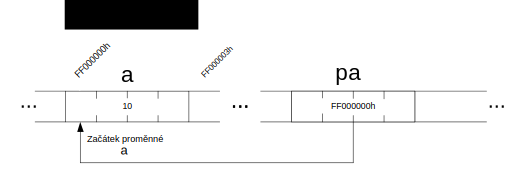
\includegraphics[width=0.9\linewidth]{princip_ukazatele.pdf}
        \caption{Princip ukazatele v paměti}
        \label{figure:pointer1}
      \end{figure}
      \begin{example}Vytvořte funkce kopírující prvky jednoho pole do druhého pomocí indexu i 
      ukazatele.
      
        % \marginpar{\includegraphics[width=0.09\textwidth]{pen.pdf}}    
        %---------------------------------------------------------------
        \lstinputlisting[caption=\texttt{CPYARRY.C} Kopíruje prvky jednoho pole do 
          druhého.]{../src/CES/C/CPYARRY.c}
        %---------------------------------------------------------------
        Výstup programu:                                                     \newline
          \lstinline[basicstyle=\ttfamily]!1   2   3   4   5   6   7   8   9!\newline
          \lstinline[basicstyle=\ttfamily]!1   2   3   4   5   6!            \newline
          \lstinline[basicstyle=\ttfamily]!4   5   6   7   8   9!            \newline
      \end{example} 

  %============= Podkapitola: Terminálový vstup a výstup============================================
  \section{Terminálový vstup a výstup}
    Jazyk C, narozdíl od Pascalu, nedefinuje žádnou \texttt{I/O (vstup\-ně/výstup\-ní 
    -In\-put/Out\-put)} operaci jako část jazyka. Nezbytné vstupy a výstupy jsou řešeny tak, že 
    standardní knihovna obsahuje několik funkcí, které \texttt{I/O} zajišťují.
  
    Nejvíce strojově závislé akce jsou I/O operace a tímto způsobem se tedy důsledně oddělují 
    strojově závislé a strojově nezávislé části jazyka. Tato skutečnost je pak významným přínosem 
    při vytváření kompilátoru pro jiný počítač.
  
    \begin{figure}[ht!]
      \centering
      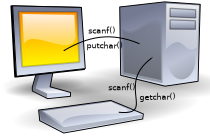
\includegraphics[scale=1.2]{terminalovy_IO_skica.pdf}
      \caption{Operace pro terminálový vstup a výstup}\label{C:fig_Terminal_IO}
    \end{figure}
  
    \subsection{Hlavičkový soubor \texttt{stdio.h}}
      Aby bylo možno správně používat všechny funkce pro vstupu a výstupu, je nutné na začátku 
      programu připojit "popis" těchto funkcí. Ten se nachází v hlavičkovém (\emph{header}) souboru 
      \lstinline[basicstyle=\ttfamily]!stdio.h!:
  
      \lstinline[basicstyle=\ttfamily]!#include <stdio.h>  //zde neni strednik!
  
      Od tohoto okamžiku je pak možné používat dále popsané funkce.
  
    \subsection{Standardní vstup a výstup znaku}
      Výstup jednoho znaku zajišťuje \lstinline[basicstyle=\ttfamily]!putchar()! a vstup jednoho 
      znaku funkce \lstinline[basicstyle=\ttfamily]!getchar()!.
      \begin{itemize}
        \item \lstinline[basicstyle=\ttfamily]!int putchar(int c);!
        \item \lstinline[basicstyle=\ttfamily]!int getchar(void);!
      \end{itemize}
      Obě funkce pracují s proměnnými \lstinline[basicstyle=\ttfamily]!int! a ne 
      \lstinline[basicstyle=\ttfamily]!char!.
  
        % \marginpar{\includegraphics[width=0.09\textwidth]{pen.pdf}}
        %---------------------------------------------------------------
        \lstinputlisting[caption=\texttt{Cteni\_tisk\_znaku.c} Čtení a tisk znak ze 
           standardního vstupu na standardní výstup.]{../src/CES/C/Cteni_tisk_znaku.c} 
        %--------------------------------------------------------------    
      
      \begin{example}Čtení znaku ze standardního vstupu a jejich zápis na standardní výstup 
        ukazuje následující program, představující jednoduchou variantu příkazu kopírování souboru 
        (nutno ovšem přesměrovat vstup a výstup).
  
        % \marginpar{\includegraphics[width=0.09\textwidth]{pen.pdf}}
        %---------------------------------------------------------------
        \lstinputlisting[caption=\texttt{CPY.c} Kopíruje znak ze standardního vstupu na 
                standardní výstup.]{../src/CES/C/CPY.c}
        %---------------------------------------------------------------
      \end{example}
      
    \subsection{Standardní vstup a výstup řetězců}
      Standardní vstup a výstup řetězců je jednoduchou nadstavbou nad čtením znaku. Obě funkce,
      \begin{itemize}
        \item \lstinline[basicstyle=\ttfamily]!char *gets(char *s);!
        \item \lstinline[basicstyle=\ttfamily]!int puts(const char *s);!
      \end{itemize}
      pracují s řetězci. \texttt{gets()} načte do znakového pole vstupní řetězec az do konce řádku, 
      symbol  \lstinline[basicstyle=\ttfamily]!'\n'! není do znakového pole zapsán. Ukazatel na 
      pole (načtený řetězec) je rovněž návratovou hodnotou. Chybu signalizuje návrat NULL. 
      \texttt{puts()} 
      zapíše řetězec na výstup a přidá přechod na novy řádek       
      \lstinline[basicstyle=\ttfamily]!'\n'!. Chybu představuje návratové \texttt{EOF}, jinak vrací 
      kladné cele číslo.
  
      Jednoduchost použití skrývá velké nebezpečí. Funkce \texttt{gets()} nemá informaci o délce 
      oblasti vymezené pro čtený řetězec. Je-li oblast kratší, než vstupní řádek, dojde jeho 
      načtením velmi pravděpodobně k přepsání paměťové oblasti související s vyhrazenou pamětí. A 
      to se všemi důsledky z toho vyplývajícími.
  
    \subsection{Formátovaný standardní vstup a vystup}
    \subsection{Souhrnné cvičení}
      \begin{example}Vytvořte program, který vygeneruje ASCII tabulku se čtyřmi sloupci ve formátu 
      \textbf{[znak|kód|znak|kód]}. Rozsah tabulky definujte pomocí dvou symbolických konstant 
      \lstinline[basicstyle=\ttfamily]!MIN_ASCII, MAX_ASCII!. 
  
        % \marginpar{\includegraphics[width=0.09\textwidth]{pen.pdf}}
        %---------------------------------------------------------------
        \lstinputlisting[caption=\texttt{ASCII.c} Generuje ASCII tabulku na terminálu.]{../src/CES/C/ASCII.c}
        %---------------------------------------------------------------
      \end{example} 

} % tikzset
%---------------------------------------------------------------------------------------------------
\printbibliography[title={Seznam literatury}, heading=subbibliography]
\addcontentsline{toc}{section}{Seznam literatury}
%  % !TeX spellcheck = cs_CZ
%{\tikzset{external/prefix={tikz/CES/}}
% \tikzset{external/figure name/.add={ch06_}{}}
%---------------------------------------------------------------------------------------------------
% file CPP.tex
%========================== Kapitola: Přehled jazyka C++============================================
\setchaptertoc
\chapter{Programování v jazyku C++}


  \section{Přehled jazyka C++}\label{CPP:IsecI}
    \texttt{C++} je rozšířená verze jazyka \texttt{C}. \texttt{C++} zahrnuje vše, co je součástí 
    jazyka \texttt{C}, a přidává podporu objektově orientovaného programování (zkráceně 
    \texttt{OOP}). \texttt{C++} navíc obsahuje mnohá vylepšení, a prvky, které z něj jednoduše 
    dělají "lepší \texttt{C}", nezávisle na objektově orientovaném programování. Kromě několika 
    málo zanedbatelných výjimek platí, že \texttt{C} je podmnožinou jazyka \texttt{C++}.

    \luagraphic[0.5]{cpp_fig001.pdf}{C++ je multiparadigmatický programovací jazyk, který vyvinul
    \emph{Bjarne Stroustrup} a další v Bellových laboratořích AT\&T rozšířením jazyka C. C++
    podporuje několik programovacích stylů (paradigmat) jako je \emph{procedurální programování},
    \emph{objektově orientované programování} a \emph{generické programování}, není tedy jazykem
    čistě objektovým. V současné době patří C++ mezi nejrozšířenější programovací jazyky.
    Kredit:Wikipedia}{cpp:fig001} 

    Účelem této kapitoly je představit některé nejdůležitější rysy jazyka C++. Prvky počítačového
    jazyka neexistují izolovaně, vzájemně spolupracují a tvoří úplný programovací jazyk.  Tato
    vzájemnost je obzvláště zřetelná u C++. Lze těžko diskutovat nějaký aspekt jazyka C++ izolovaně
    poněvadž všechny vlastnosti jazyka jsou silně propojeny. Tato kapitola přináší stručný přehled
    některých vlastností C++. Jejich přehled nám umožní porozumnět příkladům, které budou
    diskutovány v následujících kapitolách. 
  
    Poněvadž byl \texttt{C++} vytvořen pro podporu OOP, začne následující podkapitola popisem
    \texttt{OOP}. Jak uvidíme, mnoho prvků jazyka C++ má nějakým způsobem definován vztah k OOP. Je
    důležité si uvědomit, že jazyka \texttt{C++} může byt použito i pro psaní programů, které nejsou
    objektově orientovány. To, jak budemte C++ používat, závisí zcela na nás. 
    
    Tato kapitola, kromě představení nejdůležitějších vlastností jazyka \texttt{C++}, diskutuje
    rozdíly mezi způsoby programování v \texttt{C} a v \texttt{C++}. Existuje několik různých
    přístupů k jazyku C++, která dovolují větší pružnost ve způsobu psaní programů. Přestože některé
    prvky mají jen málo nebo vůbec nic co do činění s \texttt{OOP}, objevují se ve většině programů
    C++ a je vhodné diskutovat je v této knize co nejdříve. \cite[p.~20]{Schildt}.

    \begin{description}[noitemsep]
      \item[C with Classes:] Starší verze jazyka, společně označované jako \uv{C with
        Classes} (česky C s třídami), byly používány od roku 1980. Jméno C++ vymyslel Rick Mascitti
        v létě 1983. Toto jméno zdůrazňuje evoluční povahu změn oproti jazyku C; „++“ je operátor
        inkrementace v C. Kratší jméno „C+“ je syntaktická chyba a bylo též použito jako jméno
        jiného nesouvisejícího jazyka.
      \item[Standardy C++:] Přestože byl jazyk vyvíjen již od počátku 80. let, první oficiální norma
        C++ byla přijata v roce 1998, další v roce 2003 (INCITS/ISO/IEC 14882-2003). V roce 2006 a
        2007 byly přijaty některé aktualizace. Standard označovaný jako C++11, značně rozšířil C++ a
        byl přijat organizací ISO v září 2011 jako ISO/IEC 14882:2011.[1] Současný standard je C++17
        (ISO/IEC 14882:2017).
    \end{description}

    Dříve než začneme, je vhodné uvést několik všeobecných poznámek k povaze a formě jazyka C++.
    Většina součástí programů v jazyce C++ fyzicky vypadá jako programy v jazyce C. Jak programy v
    C, tak i programy v C++ začínají běh v \lstinline[style=luaCPPText]!main()!. Pro zahrnutí
    argumentů příkazového řádku používá C++ tytéž konvence \lstinline[style=luaCPPText]!argc! a
    \lstinline[style=luaCPPText]!argv! jako C. Přestože C++ definuje vlastní objektově orientované
    knihonvy, podporuje rovněž všechny funkce ve standardní knihovně jazyka C. C++ používá stejnou
    řídící strukturu jako jazyk C. C++ zahrnuje všechny zabudované datové typy definované v C. 

    \luagraphic[0.9]{cpp_fig002.jpg}{Bjarne Stroustrup (* 30. prosince 1950, Aarhus, Dánsko) je
    dánský programátor a informatik, profesor na Texas A\&M University a tvůrce programovacího jazyka
    C++.}{cpp:fig002} 

    \subsection{Co je objektově orientované programování (OOP)}
      Objektově orientované programování je výkonný způsob jak přistupovat k úloze programování. Již
      od raných začátků bylo programování spojováno s rozličnými metodologiemi. V každém kritickém
      momentě během vývoje programování byly vytvářeny nové přístupy, které pomohly programátorům
      zvládat stále složitější programy. První programy byly vytvářeny pouhým nastavením přepínačů
      na panelu počítače. Tento postup byl vhodný pouze pro velmi malé programy. Později vytvořený
      jazyk symbolických instrukcí již umožňoval psaní delších programů. K dalšímu vývoji došlo v
      roce 1955, kdy byl vytvořen první programovací jazyk vysoké úrovně - \texttt{FORTRAN}.
    
      S využitím programovacího jazyka vysoké úrovně byl programátor schopen psát programy o délce
      několika tisících řádků. Nejstarší metodou použitou pro programování byl \emph{ad hoc} přístup
      "všechno jde". Jestliže to bylo přípustné pro relativně krátké programy, pak u rozsáhlých
      programů to vedlo k vytváření nečitelných a nezvládnutelných "špagety kódů"
    
      Eliminaci "špagety kódů" umožnil až vznik \emph{strukturovaných programovacích jazyků} v
      šedesátých letech. Byly to jazyky \texttt{Algol} a \texttt{Pascal}. Volně lze interpretovat,
      že je-li jazyk C strukturovaný, pak typ programování, které v něm provádíme, by se mohl
      označit jako strukturované programování. Strukturované programování se opírá o dobře
      definované řídící struktury, bloky kódů, vyloučení příkazů GOTO, lokální (stand-alone)
      podprogramy, které podporují rekurzi, a lokální proměnné. Podstatou struktorovaného
      programování je začlenění programu do jeho základních vymezovacích prvků. S využitím
      strukturovaného programování může průměrný programátor vytvořit a udržovat program o délce až
      \num{50000} řádků. 
    
      Přestože strukturované programování přinášelo výborné výsledky, když bylo použito pro středně
      složité programy, v mnoha bodech zklamalo, když program přesáhl určitou velikost. K tomuto
      účelu bylo vytvořeno objektově orientované programování. OOP vzalo nejlepší myšlenky včleněné
      do strukturovaného programování a zkombinovalo je s výkonnými novými koncepty, které dovolují
      organizovat programy mnohem efektivněji. \texttt{OOP} podněcuje k dekompozici problému na
      základní prvky. Každá komponenta se stává samostatným a nezávislým \textbf{objektem}, který
      obsahuje své vlastní instrukce a data, vztahující se k tomuto objektu. Tímto způsobem je
      komplikovanost snížena a programátor může pracovat s rozsáhlejšímy programy. 
  
      Obecně všechny OOP jazyky sdílejí tři definované vlastnosti:

      \noindent\luafigure[1]{cpp_fig003.pdf}

      \begin{description}[noitemsep]
        \item[\textbf{Zapouzdření}:] je mechanismus, který svazuje dohromady kód a data a
          zabezpečuje je před vnějšími zásahy či před zneužitím. V objektově orientovaném jazyce
          může být kód s daty slučován takovým způsobem, že vznikají jakési nezávislé \uv{černé
          skříňky}. Spojením kódu s daty, vzniká objekt. Jinými slovy lze říci, že objekt je
          instrument, který podporuje zapouzdření.

          Uvnitř objektu může být kód nebo data nebo obojí, jednak jako \emph{privátni} (private)
          vzhledem k objektu, nebo jako \emph{veřejná} (public). Privátní kód nebo data jsou známá a
          dostupná pouze pro jinou část daného objektu. Znamená to, že privátní kód nebo data nejsou
          dosažitelné z jiné části programu mimo objekt. Když jsou kód nebo data veřejná, mohou k
          nim přistupovat i jiné části programu, přestože byly definovány uvnitř objektu. Typicky
          jsou veřejné prvky objektu využity k zajištění řízeného rozhraní k privátním elementům
          objektu.
          
          Pro libovolné účely je objekt proměnná uživatelsky definovaného typu. Může to vypadat
          podivně, že objekt, který spojuje jak kód tak i data, může být považován za proměnnou.
          Ovšem v \texttt{OOP} je tomu přesně tak. Pokaždé, když definujeme nový typ objektu,
          vytváříme nový typ dat. Každý specifický výskyt tohoto typu dat je složená proměnná.

        \item[\textbf{Polymorfismus}:] (z řeckého „mnohotvarost“) je vlastnost, která umožňuje, aby
          bylo jediné jméno použito pro dva nebo více souvisejících, ale technicky různých účelů. Ve
          vztahu k \texttt{OOP} dovoluje polymorfismus určit jedním jménem celou obecnou třídu
          procesů. Uvnitř obecné třídy procesů je pak volba konkrétního procesu dána typem dat. 

          Například v jazyce C, který nijak významně polymorfismus nepodporuje, jsou vyžadována tři
          rozdílná jména pro funkce: \lstinline[style=luaCPPText]!abs()!,
          \lstinline[style=luaCPPText]!labs()! a \lstinline[style=luaCPPText]!fabs()!. Tyto funkce
          vypočítají a vrátí absolutní hodnotu z hodnoty integer, long integer, popřípadě z hodnoty
          s pohyblivou řádovou čárkou. Protože C++ již polymorfismus podporuje, mohou být všechny
          funkce volány pod jediným jménem \lstinline[style=luaCPPText]!abs()!. (Jeden způsob, jakým
          toho lze dosáhnout, je předveden dále v této kapitole.) Typ dat použitý pro volání funkce
          pak určuje, která konkrétní verze funkce bude spuštěna. Jak uvidíme v C++, je možné použít
          jediné jméno funkce pro mnoho různých účelů. Nazývá se to vícenásobná definice funkce.

          Obecně je koncept polymorfismu charakterizován myšlenkou: \uv{jedno rozhraní, mnoho
          metod}, což znamená využití generického rozhraní pro skupiny příbuzných procedur. Výhodou
          polymorfismu je, že omezuje přílišnou složitost tím, že určením \emph{obecné třídy
          procedury} povolí jediné rozhraní. Je pak záležitostí překladače, aby vybral
          \emph{konkrétní proceduru}, vhodnou pro danou situaci. My, programátoři, nemusíme provádět
          tento výběr manuálně. Potřebujeme si pouze zapamatovat a využívat obecné rozhraní. Z
          příkladu v předchozím odstavci je zřejmé, že když pro funkci na určení absolutní hodnoty
          máme místo jediného tři jména, bude se vytvářet obecná procedura pro získání absolutní
          hodnoty podstatně složitěji, než je nezbytně nutné.

          Polymorfismus může být použit také na operátory. Ve skutečnosti všechny programovací
          jazyky obsahují pro aritmetické operátory omezenou aplikaci polymorfismu. Například v
          jazyce C je znaménko + užito k přičítání integer, long integer, znaku nebo hodnoty v
          pohyblivé řádové čárce. Ve všech případech překladač pozná, který typ aritmetiky má
          použít. V C++ můžeme tento koncept dle vlastní definice rozšířit na další typy dat. Tento
          typ polymorfismu se nazývá \emph{vícenásobná definice operátoru}.

          Klíčovým bodem, který si o polymorfismu musíme zapamatovat, je, že dovoluje vytváření
          standardního rozhraní k příslušným procesům.

        \item[\textbf{Dědičnost}:] je proces, při němž může jeden objekt získat vlastnosti jiného
          procesu. Přesněji může objekt zdědit obecnou sadu vlastnosti a do ní může přidat takové
          vlastnosti, které jsou specifické pouze pro něj. Dědičnost je důležitá, protože dovoluje
          objektu podporovat koncept hierarchické klasifikace. Většina informací je vytvářena s
          možností správy hierarchickou klasifikaci. Zkusme se například zamyslet nad popisem domu.
          Dům je částí obecné třídy nazvané budova. Budova je na oplátku zase částí obecnější třídy
          nazvané stavba, kterážto je opět součástí ještě mnohem obecnější třídy objektů zhotovených
          člověkem. V každém případě třída potomka dědí všechny vlastnosti spojené s rodiči a
          přidává k nim své vlastní charakteristiky. Bez využití uspořádané klasifikace by měl každý
          objekt definovány všechny charakteristiky, které se k němu explicitně vztahují.
          Prostřednictvím dědičnosti je však možné objekt udáním obecné třídy (nebo tříd), do které
          patří, aby si zachoval specifické vlastnosti, které jej činí jedinečným. Jak vidíme,
          dědičnost hraje v \texttt{OOP} důležitou roli. 
      \end{description}   
    \subsection{Nové hlavičky C++}
      Povšimněme si dvou řádků v následujícím programu, které jsou bezprostředně za úvodní
      poznámkou. V prvním z nich je přikaz \lstinline[style=luaCPPText]!#include!, kde již není
      \textbf{h} za jménem \lstinline[style=luaCPPText]!iostream!. V následujícím druhém řádku je
      nová specifikace prostoru jmen. Ačkoliv budou moderní hlavičky i prostor jmen detailně
      probrány dále, je nyní na řadě stručný přehled. 
      \begin{lstlisting}[style=luaCPPStyle]
        #include <iostream>
        using namespace std;

        int main()
        {
          /* programovy kod*/
          return 0;
        }
      \end{lstlisting}
      
      Jak víme, v jazyce C se při použití knihonvní funkce musí vložit její hlavičkový soubor.
      Provádí se to příkazem  \lstinline[style=luaCPPText]!#include!. Například v jazyce C vložíme
      pro zahrnutí hlavičkového soubrou I/O funkcí příkaz \lstinline[style=luaCPPText]!stdio.h!
      takto: 
      \begin{lstlisting}[style=luaCPPStyle]
        #include <stdio.h>
      \end{lstlisting}
      Zde je \lstinline[style=luaCPPText]!stdio.h! jménem souboru I/O funkce a použití příkazu
      způsobí, že se tento soubor zahrne do našeho programu. Příkaz
      \lstinline[style=luaCPPText]!#include! způsobí \emph{vložení souboru}.

      Bezprostředně po vytvoření C++ a během několika následujících let byly využívány stejné styly
      hlaviček jako v jazyce C. Standard C++ stále ještě podporuje styly hlaviček jazyka C kvůli
      zpětné kompatibilitě. Standard C++ přinesl nový druh hlaviček, který je ve standardní
      knihovně C++. Nový styl hlaviček nespecifikuje jména souborů. Místo toho se specifikují
      standardní identifikátory, které mohou být mapovány do souborů překladačem, ale také nemusí.
      Nový styl hlaviček je abstrakcí, jež jednoduše zaručuje, že byly deklarovány příslušné
      prototypy a definice požadované knihovnou C++.

      Jelikož nová hlavička není souborem, nemá příponu \textbf{h}. Taková hlavička sestává pouze ze
      jména vloženého mezi lomené závorky. Několik moderních hlaviček, které jsou podporovány
      standardem C++, je uvedeno v následujícím příkladě:
      \begin{lstlisting}[style=luaCPPStyle]
        #include <iostream>
        #include <fstream>
        #include <vector>
        #include <string>
      \end{lstlisting}

      Poněvadž C++ zahrnuje celou knihovnu funkcí jazyka C, podporuje také standardní hlavičky
      jazyka C přidružené k této knihovně. Znamená to, že jsou stále k dispozici hlavičkové soubory
      jako stdio.h a ctype.h. Ovšem standard C++ také definuje nové hlavičky, které můžete použít
      místo starých hlavičkových souborů. V jazyce C++ se ke jménu souboru původní standardní
      hlavičky jazyka C prostě ke přidá předpona \textbf{c} a odejme se \textbf{h}. Nová hlavička
      C++ pro \lstinline[style=luaCPPText]!math.c! je \lstinline[style=luaCPPText]!<cmath>! a
      hlavička pro \lstinline[style=luaCPPText]!string.h! je \lstinline[style=luaCPPText]!cstring!.
      Přestože je přípustné zahrnovat hlavičkové soubory jazyka C, když používáme knihovnu funkcí
      jazyka C, není tento přístup standardem C++ doporučován. 
      
    \subsection{Prostory jmen}
      Když do svého programu vkládáme moderní hlavičku, je obsah této hlavičky obsažen v prostoru
      jmen \lstinline[style=luaCPPText]!std!. Prostor jmen je prostě \emph{deklarativní oblast}.
      Účelem prostoru jmen je lokalizovat jména identifikátorů, a vyhnout se tak kolizím jmen.
      Tradičně byla jména z knihovny funkcí a podobné položky vkládána do globálního prostoru jmen
      (jako je to v jazyce C). Obsah nových hlaviček je umístěn v prostoru jmen
      \lstinline[style=luaCPPText]!std!. Nemusíte z nich mít obavy, protože můžete použít příkaz,
      \begin{lstlisting}[style=luaCPPStyle]
        using namespace std;
      \end{lstlisting}
      který prostor jmen \lstinline[style=luaCPPText]!std! zviditelní (tzn., že přenese
      \lstinline[style=luaCPPText]!std! do globálního prostoru jmen). Jakmile je tento příkaz
      zkompilován, setře se rozdíl mezi prací se starými a novými hlavičkami.
    
    \subsection{Konzola I/O v jazyce C++}
      Protože je C++ rozšířenou množinou jazyka C, jsou všechny prvky jazyka C obsaženy také v C++.
      Z toho vyplývá, že všechny programy C jsou zároveň programy C++. (Ve skutečnosti ovšem
      existují drobné výjimky z tohoto pravidla, které budou diskutovány dále.) Je tedy
      možné psát programy C++ jako programy C. To by samo o sobě nebylo špatné, ale nemohli bychom
      plně využívat všech výhod jazyka C++. Abychom získali maximum z výhod využívání jazyka C++,
      musíme psát nové programy ve stylu C++. To znamená využívat styly kódování a nové prvky, které
      jsou v C++ unikátní.

      Snad nejběžnějším prvkem specifickým pro C++, který je zhusta využíván, je přístup ke konzole
      I/O. Můžeme sice stále ještě využívat funkce jako \lstinline[style=luaCPPText]!printf! a
      \lstinline[style=luaCPPText]!scanf!, ale C++ nám nabízí nový a lepší způsob, jak provádět tyto
      typy I/O operací. V jazyce C++ jsou I/O operace namísto I/O funkcí prováděny pomocí I/O
      operátorů. \textbf{Výstupní operátor} je \lstinline[style=luaCPPText]!<<! a \textbf{vstupní
      operátor} je \lstinline[style=luaCPPText]!>>!. Jak víme, v C slouží tyto operátory jako
      \emph{levý} a \emph{pravý shift}. V jazyce C++ stále ještě přetrvává jejich původní význam
      (levý a pravý shift), ale zároveň přijímají novou rozšířenou roli pro provádění vstupů a
      výstupů. Povšimněme si následujícího příkazu C++:
      \begin{lstlisting}[style=luaCPPStyle]
        cout << "This string is output to the screen. \n";
      \end{lstlisting}
      Tento příkaz způsobí, že se na obrazovce počítače zobrazí řetězec.
      \lstinline[style=luaCPPText]!cout! je předdefinovaný datový proud (stream), který je při
      spuštění programu C++ automaticky připojen ke konzole. Je to podobné jako
      \lstinline[style=luaCPPText]!stdout! v jazyce C. Stejně jako v C může být i v C++ konzola
      přesměrována, ale budeme předpokládat, že je používána. Při použití výstupního operátoru
      \lstinline[style=luaCPPText]!<<! lze provést výstup jakéhokoliv základního typu jazyka C++:
      \begin{lstlisting}[style=luaCPPStyle]
        cout << 100.99;
      \end{lstlisting}
      Obecně platí, že pro výstup na konzolu se používá tato forma operátoru
      \lstinline[style=luaCPPText]!<<!:
      \begin{lstlisting}[style=luaCPPStyle]
        cout << expression; 
      \end{lstlisting}
      Pojmem \emph{výraz} (expression) se míní jakýkoliv platný výraz jazyka C++ včetně dalšího
      výstupního výrazu.

      Pro vstup hodnoty z klávesnice používejme vstupní operátor \lstinline[style=luaCPPText]!>>!.
      Například následující fragment obslouží vstup integer hodnoty do
      \lstinline[style=luaCPPText]!num!.
      \begin{lstlisting}[style=luaCPPStyle]
        int num; 
        cin >> num; 
      \end{lstlisting}
      Povšimněme si, že před \lstinline[style=luaCPPText]!num! není znak
      \lstinline[style=luaCPPText]!&!. Víme, že když pro vstup hodnoty použijeme  \uv{céčkovou}
      funkci \lstinline[style=luaCPPText]!scanf()!, musí funkce nejprve získat adresy proměnných,
      aby ty pak mohly přijmout hodnoty vložené uživatelem. Toto však není nutné, když použijeme
      vstupní operátor C++\footnote{Proč to tak je, se objasní, jakmile se dozvíme víc o C++.}.  
      
      \begin{mdframed}[style=highlight] 
        Rozšířené role operatoru \lstinline[style=luaCPPText]!<<! a
        \lstinline[style=luaCPPText]!>>! je příkladem přetěžování operátoru.
      \end{mdframed}

      Pro používání I/O operátorů v jazyce C++ musíme do programu zařadit hlavičku 
      \lstinline[style=luaCPPText]!<iostream>!. Jak již bylo dříve vysvětleno, je to jedna ze
      standardních hlaviček C++.

      %--iostream-----------------------------------------------------
        % !TeX spellcheck = cs_CZ
\begin{mdframed}[style=mdexam]
  \begin{example}\label{cpp:exam003}
    Výstupem z tohoto programu je řetězec, dvě hodnoty integer a hodnota v rozšířené pohyblivé
    řádové čárce: 
    %---------------------------------------------------------------
      \begin{lstlisting}[style=luaCPPStyle]
        #include <iostream> 
        using namespace std;
        
        int main()
        {
          int i, j; 
          double d;

          i = 10; 
          j = 20; 
          d = 99.101;
          
          cout << "Here are some values: "; 
          cout << i; 
          cout << ' '; 
          cout << j;
          cout << ' '; 
          cout << d;

          return 0;
        }
      \end{lstlisting}
    %---------------------------------------------------------------
    Výstup z programu bude vypadat takto: 
    \begin{mdframed}[style=mdmsdos]
      Here are some values: 10 20 99.101
    \end{mdframed}

    V jediném I/O výrazu je možné provést výstup více než jedné hodnoty. 
      %---------------------------------------------------------------
      \begin{lstlisting}[style=luaCPPStyle]
        cout << i << ' ' << j << ' ' << d;
      \end{lstlisting}
    %---------------------------------------------------------------
    Povšimněme si, že mezi položky musíme explicitně vložit mezery. Když mezera chybí, neoddělená
    data se při zobrazení na obrazovce spojí.
  \end{example}
\end{mdframed}
      %---------------------------------------------------------------

      %--iostream-cin-------------------------------------------------
        % !TeX spellcheck = cs_CZ
\begin{mdframed}[style=mdexam]
  \begin{example}\label{cpp:exam004}
   Tento program vybídne uživatele ke vložení hodnoty integer:
    %---------------------------------------------------------------
      \begin{lstlisting}[style=luaCPPStyle]
        #include <iostream> 
        using namespace std;
        
        int main()
        {
          int i;

          cout << "Enter a value: "; 
          cin >> i;
          cout << "Here's your number: " << i << "\n";

          return 0;
        }
      \end{lstlisting}
    %---------------------------------------------------------------
    Zde je příklad běhu programu:
    \begin{mdframed}[style=mdmsdos]
      Enter a value: 100 \newline
      Here's your number: 100
    \end{mdframed}  
    Hodnota vložená uživatelem je, jak vidíte, předána do \texttt{i}. 

    Program nyní trochu zmodifikujeme tak, aby uživatele vybídla ke vložení hodnoty integer,
    hodnoty v pohyblivé řádové čárce a řetězce. Vše v jediném vstupním příkazu.
    %---------------------------------------------------------------
      \begin{lstlisting}[style=luaCPPStyle]    
        int main()
        {
          int i; 
          float f; 
          char s[80];

          cout << "Enter an integer, float, and string: "; 
          cin >> i >> f >> S; 
          cout << "Here's your data: "; 
          cout << i << ' ' << f «< ' « s;

          return 0;
        }
      \end{lstlisting}
    %---------------------------------------------------------------   
    Tento příklad ilustruje, že v jediném příkazu může vstupovat libovolný počet položek. Stejně
    jako v C musí být položky odděleny vhodnými oddělovacími znaky (mezery, tabelátory nebo konec
    řádku).  

    Při načítání řetězce se vstup zastaví v okamžiku, kdy se objeví první oddělovací znak. Když
    například vložíte do předchozího programu následující data 
    \begin{mdframed}[style=mdmsdos]
      10 100.12 This is a test
    \end{mdframed}  
    zobrazí program toto:
    \begin{mdframed}[style=mdmsdos]
      10 100.12 This
    \end{mdframed}  
    Řetězec není úplný, protože se jeho načítání zastavilo na mezeře za \texttt{This}. Zbytek
    řetězce zůstal ve vstupním bufferu a čeká na další vstupní operaci. (Je to podobné, jako když
    vstupuje řetězec s využitím \lstinline[style=luaCPPText]!scanf()! ve formátu \texttt{\%s}.)   
  \end{example}
\end{mdframed}
      %---------------------------------------------------------------

      Standardně, když použijeme \lstinline[style=luaCPPText]!>>!, jdou všechny vstupy přes
      vyrovnavací paměť. Znamená to, že se do našeho programu C++ nedostane žádná informace, pokud
      nestisknete \texttt{ENTER}. (V jazyce C je funkce \lstinline[style=luaCPPText]!scanf()!
      zpracovávána po řádcích, takže by tento styl práce se vstupem pro nás neměl být nový.) Abychom
      viděli efekt vstupu přes řádkovou vyrovnávací paměť, vyzkoušejme následující program:
      %---------------------------------------------------------------
      \begin{lstlisting}[style=luaCPPStyle]    
        int main()
        {
          char ch;

          cout << "Enter keys, x to stop. \n";
        
          do {
            cout << ": ";
            cin >> ch; 
          } while (ch != 'x');  

          return 0;
        }
      \end{lstlisting}
      %---------------------------------------------------------------  
      Když budeme program zkoušet, budeme muset mačkat \texttt{ENTER} po stisku každé klávesy, aby
      byl vložený znak předán programu.

    \subsection{Třídy: první nahlédnutí}
      Snad nejdůležitějším samostatným prvkem jazyka C++ je \textbf{třída}. Je to mechanismus
      používaný pro vytváření objektů. Jako taková, je třída srdcem mnoha prvků jazyka C++. Třídy
      jsou pro programování v C++ tak významné, že je vhodné předložit na tomto místě jejich stručný
      přehled.
      
      \begin{mdframed}[style=highlight]
        \textbf{Třída} je základním obecným pojmem klasifikace, jak při návrhu uspořádávat informace 
        do smysluplné entity. Základním pojmem je \emph{objekt}, \textbf{instance třídy}, jako 
        konkrétní případ realizace předpisu. Objekt si „pamatuje“ svůj stav (v podobě \textbf{dat} 
        čili \textbf{atributů}) a zveřejněním některých svých operací (nazývaných \textbf{metody}) 
        poskytuje rozhraní, jak s ním pracovat. Při používání objektu nás zajímá, jaké operace 
        (služby) poskytuje, ale ne, jakým způsobem to provádí - to je princip \emph{zapouzdření}. 
        Jestli to provádí sám nebo využije služeb jiných objektů, je celkem jedno. Vlastní 
        implementaci pak můžeme změnit (např. zefektivnit), aniž by se to dotklo všech, kteří 
        objekt používají.
      \end{mdframed}
       
      Abstrakce objektu, která v architektuře programu podchycuje na obecné úrovni podstatu všech
      objektů podobného typu, se nazývá \textbf{třída}. Třída je předpis, jak vyrobit objekt daného
      typu.
  
      Třída je deklarována klíčovým slovem \lstinline[style=luaCPPText]!class!. Syntaxe deklarace
      \lstinline[style=luaCPPText]!class! je podobná její struktuře. V obecné formě vypadá takto
  
      %---------------------------------------------------------------
      \begin{lstlisting}[style=luaCPPStyle]
        class jméno-třídy{
          // privatni-funkce a promenne
        public:
          // verejné funkce a promenne
        } seznam-objektů
      \end{lstlisting}
      %---------------------------------------------------------------
      Seznam objektů je v deklaraci třídy nepovinný. Stejně jako struktura, se  mohou  objekty 
      třídy deklarovat později. Zatímco jméno třídy je také nepovinné, z praktického hlediska je 
      vlastně vždy potřeba. Je to proto, že se jméno třídy stává novým typem jména použitého k 
      deklaraci objektů třídy.
  
      \textbf{Funkce a proměnné} deklarované uvnitř třídy jsou označeny jako \textit{členy této 
      třídy}. Znamená to, že jsou přístupné pouze pro ostatní členy třídy. Pro deklaraci členů 
      veřejné třídy se použije klíčové slovo \lstinline[style=luaCPPText]!public! s dvojtečkou. 
      Všechny funkce a proměn\-né deklarované za tímto specifikátorem jsou přístupné jak pro členy 
      třídy, tak i pro další části programu, které obsahují třídu.
  
      Toto je jednoduchá deklarace třídy:
  
      %---------------------------------------------------------------
      \begin{lstlisting}[style=luaCPPStyle]
        class myclass{
          // privátní vzhledem k myclass
          int a;
        public:
          void set_a(int num);
          int get_a();
        };
      \end{lstlisting}
      %---------------------------------------------------------------
      Tato třída má pouze jednu privátní proměnnou nazvanou \lstinline[style=luaCPPText]!a! a 
      dvě veřejné funkce \lstinline[style=luaCPPText]!set_a()! a 
      \lstinline[style=luaCPPText]!get_a()!. Tyto funkce jsou deklarovány uvnitř třídy pomocí 
      jejich \textbf{prototypů}. Funkce, které jsou deklarovány jako součásti třídy se nazývají 
      \textit{členské funkce}.
  
      Jelikož je \lstinline[style=luaCPPText]!a! privátní, není dostupné pro žádný kód vně
      \lstinline[style=luaCPPText]!myclass!. Ovšem funkce \lstinline[style=luaCPPText]!set_a()! a
      \lstinline[style=luaCPPText]!get_a()! jsou členy \lstinline[style=luaCPPText]!myclass!, takže
      mají k \lstinline[style=luaCPPText]!a! přístup. \lstinline[style=luaCPPText]!set_a()! a
      \lstinline[style=luaCPPText]!get_a()! jsou deklarovány jako veřejné členy
      \lstinline[style=luaCPPText]!myclass! a mohou být volány každou částí programu, která
      \lstinline[style=luaCPPText]!myclass! obsahuje.
  
      Ačkoliv jsou funkce \lstinline[style=luaCPPText]!set_a()! a
      \lstinline[style=luaCPPText]!get_a()!  deklarovány v \lstinline[style=luaCPPText]!myclass!,
      nejsou ještě definovány. Aby jsem definoval členskou funkci, musím spojit typové jméno třídy
      se jménem funkce. To se udělá uvozením jména funkce jménem třídy se dvojicí dvojteček. Dvojice
      dvojteček se nazývá \textit{operátor rozlišení oblasti} (scope resolution operator).
      Následující příklad ukazuje, jak jsou členské funkce \lstinline[style=luaCPPText]!set_a()! a
      \lstinline[style=luaCPPText]!get_a()! definovány:
      %---------------------------------------------------------------
      \begin{lstlisting}[style=luaCPPStyle]
        void myclass::set_a(int num){
          a = num;
        }
    
        int myclass::get_a(){
          return a;
        }
      \end{lstlisting}
      %---------------------------------------------------------------
      Jak \lstinline[style=luaCPPText]!get_a()!, tak i \lstinline[style=luaCPPText]!set_a()! mají
      přístup k \lstinline[style=luaCPPText]!a!, které je privátní v
      \lstinline[style=luaCPPText]!myclass!. Poněvadž \lstinline[style=luaCPPText]!get_a()! i
      \lstinline[style=luaCPPText]!set_a()! jsou členy \lstinline[style=luaCPPText]!myclass!, mohou
      přímo přistupovat k jejím soukromým datům.
  
      Obecně se pro definici členské funkce musí použít následující tvar:
      %---------------------------------------------------------------
      \begin{lstlisting}[style=luaCPPStyle]
        retype jmeno-tridy::jmeno-funkce(seznam-parametru)
        {
        // telo funkce
        }
      \end{lstlisting}
      %---------------------------------------------------------------
      Zde je \texttt{jmeno-tridy} jménem třídy, do níž funkce  náleží.

      Deklarace \lstinline[style=luaCPPText]!myclass! nedefinuje žádný objekt typu
      \lstinline[style=luaCPPText]!myclass!. Definuje pouze typ objektu, který bude vytvořen, když
      bude deklarován. Pro vytvoření objektu se použije jako specifikátor jméno třídy. Například
      tento řádek deklaruje dva objekty typu \lstinline[style=luaCPPText]!myclass!:
      %---------------------------------------------------------------
      \begin{lstlisting}[style=luaCPPStyle]
        myclass ob1, ob2; //toto jsou objekty typu myclass
      \end{lstlisting}
      %---------------------------------------------------------------

      \begin{mdframed}[style=highlight]
        Deklarace třídy je pouze logická abstrakce, jež definuje nový typ. Určuje, jak bude objekt
        daného typu vypadat. Teprve deklarace objektu vytváří fyzickou entitu daného typu. Objekt
        totiž zabírá pamět, ale definiční typ ne.
      \end{mdframed}

      Jakmile je vytvořen objekt třídy, může se program odkazovat na jeho veřejné členy pomocí
      tečkových operátorů bezmála takovým způsobem, jímž jsou prvky struktury zpřístupněny. Dle
      předcházející deklarace objektů volají následující příkazy
      \lstinline[style=luaCPPText]!set_a()! pro objekty \lstinline[style=luaCPPText]!ob1! a
      \lstinline[style=luaCPPText]!ob2!:
      %---------------------------------------------------------------
      \begin{lstlisting}[style=luaCPPStyle]
        ob1.set_a(10); // nastaví verzi ob1 na 10
        ob2.set_a(99); // nastaví verzi ob2 na 99
      \end{lstlisting}
      %---------------------------------------------------------------
      Jak vysvětlují poznámky, tyto příkazy nastavují kopii \lstinline[style=luaCPPText]!ob1! z
      \lstinline[style=luaCPPText]!a! na \lstinline[style=luaCPPText]!10! a kopii
      \lstinline[style=luaCPPText]!ob2! na \lstinline[style=luaCPPText]!99!. Každý objekt obsahuje
      vlastní kopii všech dat deklarovaných uvnitř třídy. Znamená to, že
      \lstinline[style=luaCPPText]!a! náležející \lstinline[style=luaCPPText]!ob1! je odlišné a
      různé od \lstinline[style=luaCPPText]!a! navázaného na \lstinline[style=luaCPPText]!ob2!

      \begin{mdframed}[style=highlight]
        Každý objekt obsahuje vlastní kopii všech dat deklarovaných uvnitř třídy. 
      \end{mdframed}

      %--Nechť má sousedka (chápejme ji jako objekt) má nějaké jméno--
      % !TeX spellcheck = cs_CZ
\begin{mdframed}[style=mdexam]
  \begin{example}\label{cpp:exam002}
    Tento program předvádí \lstinline[basicstyle=\ttfamily]!myclass!, popsanou výše v textu. 
    Nastavuje hodnoty \lstinline[basicstyle=\ttfamily]!a! pro 
    \lstinline[basicstyle=\ttfamily]!ob1! a 
    \lstinline[basicstyle=\ttfamily]!ob2!, a pak zobrazuje hodnotu a pro každý objekt.
    % \marginpar{\includegraphics[width=0.05\textwidth]{pen.pdf}}
    \vspace{1em}       
    %---------------------------------------------------------------
    \lstinputlisting[style=luaCPPStyle, caption={\texttt{HS\_37\_myclass.cpp}: představení třídy 
    \texttt{myclass}.}]{../src/CES/CPP/HS_37_myclass.cpp}
    %---------------------------------------------------------------
    Program by měl na obrazovce zobrazit hodnoty \lstinline[basicstyle=\ttfamily]!10! a 
    \lstinline[basicstyle=\ttfamily]!99!.
  \end{example}
\end{mdframed}
      %---------------------------------------------------------------

      V \lstinline[style=luaCPPText]!myclass! z předchozího příkladu je
      \lstinline[style=luaCPPText]!a! privatní. Znamená to, žek ní mohou přímo přistupovat pouze
      členské funkce z \lstinline[style=luaCPPText]!myclass!. (To je důvodem, proč je vyžadována
      veřejná funkce \lstinline[style=luaCPPText]!get_a()!). Jestliže se pokusíme o přístup k
      privátnímu členu třídy z některé části svého programu, který není členem třídy, objeví se při
      překladu chyba. předpokládejme například, že je \lstinline[style=luaCPPText]!myclass!
      definována tak, jak bylo předvedeno v předešlém příkladě. Pak následující volání funkce
      \lstinline[style=luaCPPText]!main()! zapříčiní chybu: 
      %---------------------------------------------------------------
      \begin{lstlisting}[style=luaCPPStyle]
        // Toto je fragment obsahující chybu.
        #include<iostream>
        using namespace std;
        int main()
        {
          myclass ob1, ob2;
          ob1.a = 10; // ERROR! nemuze pristupovat
                      // k privatnimu clenu
          ob2.a = 99; // dle neclenskych funkci.

          cout << ob1.get_a() << "\n";
          cout << ob2.get_a() << "\n";

          return 0;
        }
      \end{lstlisting}
      %---------------------------------------------------------------

      Stejně jako mohou existovat funkce veřejného členu, mohou existovat i proměnné veřejného 
      členu. Jestliže například \lstinline[style=luaCPPText]!a! bylo deklarováno ve veřejné 
      části \lstinline[style=luaCPPText]!myclass!, lze se na ně odkazovat z kterékoliv části 
      programu, jak je předvedeno dále:
      % \marginpar{\includegraphics[width=0.09\textwidth]{pen.pdf}}
      %---------------------------------------------------------------
        \begin{lstlisting}[style=luaCPPStyle]
          #include<iostream>
          using namespace std;
  
          class myclass{
          public:
          // nyní je a veřejné
          int a;
          // a  nyní není potřeba set_a() a get_a()
          };
  
          int main()
          {
          myclass ob1, ob2;
  
          ob1.a = 10;
          ob2.a = 99;
  
          cout << ob1.a << "\n";
          cout << ob2.a << "\n";
  
          return 0;
          }
        \end{lstlisting}
      %---------------------------------------------------------------
      Protože je v tomto příkladě \lstinline[style=luaCPPText]!a! deklarováno jako veřejný 
      člen \lstinline[style=luaCPPText]!myclass!, je přímo přístupné z 
      \lstinline[style=luaCPPText]!main()!. Pro přístup k \lstinline[style=luaCPPText]!a! 
      je použit tečkový operátor. Obvykle, když se volá členská funkce nebo se přistupuje k 
      členské proměnné z vnějšího prostředí mimo třídu, je nutná plná specifikace daná jménem 
      objektu i s tečkovým operátorem následovaným jménem člena, aby bylo jasné, na kterého člena 
      objektu se odkazuje.

      Aby byla ukázána síla objektů, následující program \ref{cpp:exam006} vytváří třídu
      pojmenovanou \lstinline[style=luaCPPText]!stack!, která implementuje zásobník použitelný
      například pro uchování znaků:

      %--stack -------------------------------------------------------
      % !TeX spellcheck = cs_CZ
\begin{mdframed}[style=mdexam]
  \begin{example}\label{cpp:exam006}
    Vytvoř třídu \lstinline[style=luaCPPText]!stack!, která implementuje zásobník použitelný pro
    uchování znaků:
    %---------------------------------------------------------------
    \lstinputlisting[style=luaCPPStyle]{../src/CES/CPP/HS_39_stack.cpp}
    %---------------------------------------------------------------
    Program zobrazí následující výstupy:
    \begin{mdframed}[style=mdmsdos]
    Pop s1: c\newline
    Pop s1: b\newline
    Pop s1: a\newline
    Pop s2: z\newline
    Pop s2: y\newline
    Pop s2: x
    \end{mdframed}
  \end{example}
\end{mdframed}
      %---------------------------------------------------------------

      Podívej se na program \ref{cpp:exam006} ještě jednou. Třída
      \lstinline[style=luaCPPText]!stack! obsahuje dvě privátní proměnné:
      \lstinline[style=luaCPPText]!stck! a \lstinline[style=luaCPPText]!tos!. Pole
      \lstinline[style=luaCPPText]!stck! uchovává znaky umístěné v zásobníku a
      \lstinline[style=luaCPPText]!tos! obsahuje index horní úrovně zásobníku. Veřejné funkce
      zásobníku jsou 
      \begin{itemize}[noitemsep]
        \item \lstinline[style=luaCPPText]!init()!,
        \item \lstinline[style=luaCPPText]!push()! a
        \item \lstinline[style=luaCPPText]!pop()!
      \end{itemize}       
      a slouží k inicializaci zásobníku, vkládání hodnoty a k vyjmutí hodnoty. 
      
      Uvnitř funkce \lstinline[style=luaCPPText]!main()! jsou vytvořeny dva zásobníky
      \lstinline[style=luaCPPText]!s1! a \lstinline[style=luaCPPText]!s2! a do každého z nich jsou
      vloženy tři znaky. Je důležité uvědomit si, že každý zásobníkový objekt je oddělený od
      druhého. To znamená, že znaky vložené do \lstinline[style=luaCPPText]!s1! nemohou žádným
      způsobem ovlivnit znaky vložené do \lstinline[style=luaCPPText]!s2!. Každý objekt obsahuje
      vlastní kopii \lstinline[style=luaCPPText]!stck! a \lstinline[style=luaCPPText]!tos!. To je
      základní princip pro pochopení objektů. Ačkoliv všechny objekty třídy sdílejí své členské
      funkce, každý objekt vytváří a udržuje svá vlastní data.
  
    \subsection{Některé rozdíly mezi C a C++}
      Ačkoliv je jazyk C++ rozšířenou množinou jazyka C, existují mezi nimi drobné rozdíly a bylo by
      dobré se s nimi na začátku seznámit. 
      
      Především, když v C nemá funkce žádné parametry, její protyp má v seznamu parametrů funkce
      slovo \lstinline[style=luaCPPText]!void!. Například když v "céčku" funkce nazvaná
      \lstinline[style=luaCPPText]!fl()! nemá parametry (a vrací
      \lstinline[style=luaCPPText]!char!), pak její prototyp bude vypadat následovně:
      %---------------------------------------------------------------
      \begin{lstlisting}[style=luaCPPStyle]
        char fl(void);
      \end{lstlisting}
      %---------------------------------------------------------------
      Přestože v C++ zůstává \lstinline[style=luaCPPText]!void! stále jako volitelný, bude se
      prototyp pro \lstinline[style=luaCPPText]!fl()! psát běžně takto:
      %---------------------------------------------------------------
      \begin{lstlisting}[style=luaCPPStyle]
        char fl();
      \end{lstlisting}
      %---------------------------------------------------------------
  
      C++ se odlišuje od C tím, že je v něm specifikován prázdný seznam parametrů. Kdyby se
      předchozí prototyp objevil v programu C, pak se to bude chápat, že o parametrech nebylo řečeno
      nic. V C++ to znamená, že funkce nemá parametry. Proto tedy v předchozím příkladě nebyl využit
      k deklaraci prázdného seznamu explicitně parametr \lstinline[style=luaCPPText]!void!. (Použití
      parametru void k deklaraci prázdného  seznamu parametrů není zakázáno; je to pouze nadbytečné.
      Jelikož většina programů C++ usiluje o téměř posvátným zanícením o výkonnost,neuvidíme téměř
      nikdy, že by bylo \lstinline[style=luaCPPText]!void! tímto způsobem použito.) Zapamatujme si,
      že v C++ jsou následující dvě deklarace zcela rovnocenné:
      %---------------------------------------------------------------
      \begin{lstlisting}[style=luaCPPStyle]
        char fl();
        char fl(void);
      \end{lstlisting}
      %---------------------------------------------------------------
  
      Další drobná diference mezi C a C++ spočívá v tom, že v programech C++ musí mít všechny 
      funkce prototypy. Zapamatujme si, že v C jsou prototypy doporučeny, ale technicky jsou 
      nepovinné. V C++ jsou však vyžadovány. Jak je patrno z příkladu v předchozí části, prototyp 
      členské funkce obsažený v třídě slouží rovněž jako její obecný prototyp a žádný další 
      samostatný prototyp již není požadován. 
      
      Třetím rozdílem mezi C a C++ je, když je funkce deklarována aby vracela hodnotu, musí hodnotu
      opravdu vracet. Jestliže má totiž funkce jiný návratový typ než
      \lstinline[style=luaCPPText]!void!, musí pak každý příkaz \lstinline[style=luaCPPText]!return!
      uvnitř funkce obsahovat hodnotu. V C není vyžadováno, aby vracely hodnotu funkce, které nejsou
      \lstinline[style=luaCPPText]!void!. Jestliže hodnota neexistuje, "vrací se" jakási nahodilá
      hodnota.
   
      Jestliže v C nespecifikujete explicitně návratový typ funkce, předpokládá se návratový typ
      \lstinline[style=luaCPPText]!integer!. V C++ bylo toto pravidlo potlačeno, a proto musíme
      explicitně deklarovat všechny návratové typy funkcí. Další rozdíl mezi C a C++ je, že v
      programech C budeme muset brát ohled na to, kde mohou být lokální proměnné deklarovány. V C
      mohou být lokální proměnné deklarovány pouze na začátku bloku před všemi "výkonnými" příkazy.
      V C++ mohou být lokální proměnné deklarovány kdekoliv. Výhodou tohoto přístupu je, že lokální
      proměnné mohou být deklarovány tam, kde budou poprvé použity, což může napomoci v prevenci
      před nechtěnými vedlejšími účinky.
  
      Konečně také v C++ definuje datový typ \lstinline[style=luaCPPText]!bool! pro uložení hodnot
      \lstinline[style=luaCPPText]!Boolean! (popř. pravda/nepravda). C++ rovněž definuje klíčová
      slova \lstinline[style=luaCPPText]!true! a \lstinline[style=luaCPPText]!false!, která jsou
      jedinými hodnotami, které může hodnota typu \lstinline[style=luaCPPText]!Boolean! nabývat. V
      C++ je výstupní hodnotou relačních a logických operátorů hodnota typu
      \lstinline[style=luaCPPText]!bool! a všechny podmíněné příkazy musí hodnotu bool vyhodnocovat.
      V C je hodnota \lstinline[style=luaCPPText]!true! nenulová a hodnota
      \lstinline[style=luaCPPText]!false! odpovídá nule. Tak je to i v C++, poněvadž při použití v
      booleánských výrazech je každá nenulová hodnota automaticky převedena na
      \lstinline[style=luaCPPText]!true! a každá nulová hodnota je převedena na
      \lstinline[style=luaCPPText]!false!. Funguje to i opačným směrem. Když je booleánská hodnota
      použita ve výrazech \lstinline[style=luaCPPText]!integer!, pak se
      \lstinline[style=luaCPPText]!true! převádí na \lstinline[style=luaCPPText]!1! a
      \lstinline[style=luaCPPText]!false! na \lstinline[style=luaCPPText]!0!. Přidání
      \lstinline[style=luaCPPText]!bool! umožňuje důkladnější ověřování typů a poskytuje způsob, jak
      navzájem rozlišovat \lstinline[style=luaCPPText]!Boolean! a
      \lstinline[style=luaCPPText]!integer!. Využívání je samozřejmě nepovinné, ale
      \lstinline[style=luaCPPText]!bool! je nejpohodlnější.
  
    \subsection{Úvod do přetěžování funkcí}
      Po třídách je snad nejdůležitější a vše prostupující vlastností C++ přetě\-žování funkcí. 
      Přetěžování funkcí nejen poskytuje mechanismus jímž C++ poskytuje jeden typ polymorfismu, ale 
      také utváří základ, na němž může být programovací prostředí dynamicky rozšiřováno. Kvůli 
      důležitosti přetěžování je v následujících odstavcích předložen stručný úvod. \footnote{V C++ 
      lze přetěžovat i operátory.}
  
      V C++ mohou dvě nebo více funkcí sdílet stejné jméno, pokud se liší typy jejich argumentů 
      nebo jejich počet anebo se liší obojí.
  
      Je velmi snadné přetížit funkci: jednoduše deklarujeme a definujeme všechny požadované verze. 
      Správnou verzi překladač automaticky vybere dle počtu nebo typu argumentů použitých při 
      volání funkce.

      Jedním z hlavních použití přetětovaných funkcí je dosažení \emph{polymorfismu} kompilace,
      který ztělesňuje filosofii: \textbf{jedno rozhraní, mnoho metod}. Jak víme, je běžné mít při
      programování v \uv{céčku} více příbuzných funkcí, které se odlišují pouze typem zpracovávaných
      dat. Klasický příklad této situace lze nalézt ve standardní knihovně C. jak již bylo zmíněno
      dříve v této kapitole, knihovna obsahuje funkce \lstinline[style=luaCPPText]!abs()!,
      \lstinline[style=luaCPPText]!labs()! a \lstinline[style=luaCPPText]!fabs()!, které vracejí
      absolutní hodnotu z \lstinline[style=luaCPPText]!integer!,
      \lstinline[style=luaCPPText]!long integer! nebo z formátu s pohyblivou řádovou čárkou. 

      Přestože jsou kvůli třem různým typům dat požadována tři různá jména, je situace 
      komplikovanější víc, než je nutné. Ve všech třech případech se vrací absolutní hodnota; liší
      se pouze typ dat. V C++ můžeme tuto situaci upravit přetížením jednoho jména pro tři typy dat,
      jak ukazuje následující příklad:  
      %--{cpp:exam007}-abs--------------------------------------------
      % !TeX spellcheck = cs_CZ
\begin{mdframed}[style=mdexam]
  \begin{example}\label{cpp:exam007}
    Definujme tři funkce pro výpočet absolutní hodnoty nazvané \lstinline[style=luaCPPText]!abs()! -
    pro každý typ dat jednu.
    %---------------------------------------------------------------
    \lstinputlisting[style=luaCPPStyle]{../src/CES/CPP/HS_46_abs.cpp}
    %---------------------------------------------------------------
  \end{example}
\end{mdframed}
      %---------------------------------------------------------------
      Vidíme, že tento program definuje tři funkce nazvané \lstinline[style=luaCPPText]!abs()! - pro
      každý typ dat jednu. Uvnitř \lstinline[style=luaCPPText]!main()! je funcke
      \lstinline[style=luaCPPText]!abs()! volána s použitím tří různých typů argumentů.
      Překladač automaticky volá správně jednu ze tří verzí \lstinline[style=luaCPPText]!abs()! dle
      typu dat, která jsou uvedena v argumentu. Program vytvoří následující výstup:
      \begin{mdframed}[style=mdmsdos]
        In integer abs()\newline
        Absolute value of -10: 10\newline\vspace{1em}  
        In long abs()   \newline
        Absolute value of -10L: 10\newline\vspace{1em}  
        In double abs() \newline
        Absolute value of -10.01: 10.01
      \end{mdframed}

      Uvedený příklad je velmi jednoduchý, nicméně ukazuje význam přetěžování funkcí. Jelikož lze
      jediné jméno použít k popisu obecné třídy činností, je umělá složitost, která vyplývá z
      použití tří mírně odlišných jmen - v tomto případě \lstinline[style=luaCPPText]!abs()!,
      \lstinline[style=luaCPPText]!labs()! a \lstinline[style=luaCPPText]!fabs()! - snadno
      eliminována. Nyní si musíme zapamatovat pouze jediné jméno, které popisuje \emph{obecnou}
      činnost. zůstává pak na překladači, aby si zvolil vhodnou druhovou verzi funkce (tzn. metodu).
      Je to přínos pro snížení složitosi. Tedy - díky použití polymorfismu byla tři jména omezena na
      jedno. 

      Zatímco v příkladě \ref{cpp:exam007} je použití polymorfismu poměrně jednoduché, měli bychom
      být schopni uvědomit si, jak efektivní může být ve velmi rozsáhlém programu přístup \uv{jedno
      rozhraní - mnoho metod}. 

      Následující příklad \ref{cpp:exam008} ukazuje přetížení funkce
      \lstinline[style=luaCPPText]!date()!.
      %--{cpp:exam008}-date------------------------------------------
      % !TeX spellcheck = cs_CZ
\begin{mdframed}[style=mdexam]
  \begin{example}\label{cpp:exam008}
    Vytvořte funkci \lstinline[style=luaCPPText]!date()!, aby byla schopna přijmout datum buď jako
    řetězec nebo jako tři hodnoty \lstinline[style=luaCPPText]!integer!. V obou případech pak funkce
    zobrazí vložené datum.
    %---------------------------------------------------------------
    \lstinputlisting[style=luaCPPStyle]{../src/CES/CPP/HS_47_date.cpp}
    %---------------------------------------------------------------
  \end{example}
\end{mdframed}
      %---------------------------------------------------------------
    
      Příklad \ref{cpp:exam008} ilustruje jak může přetížení funkce zajistit mnohem při\-rozenější
      přístup k funkci. Protože je poměrně běžné, že je datum reprezentováno buď řetězcem, nebo
      třemi celočíselnými hodnotami obsahující den, měsíc a rok, záleží jen na uživateli, aby vybral
      tu nejpohodlnější formu, dle dané situace
  
    \subsection{Práce s ukazateli} 
      
      %--{cpp:exam009}-Práce s ukazateli-------------------------------
      % !TeX spellcheck = cs_CZ
\begin{mdframed}[style=mdexam]
  \begin{example}\label{cpp:exam009}
    Práce s ukazateli:
    %---------------------------------------------------------------
    \lstinputlisting[style=luaCPPStyle]{../src/CES/CPP/GP_548_point.cpp}
    %---------------------------------------------------------------
    Výstup programu:
    \begin{mdframed}[style=mdmsdos]
      num is 123  \newline
      The address of num is 0x28ff44 \newline
      *p\_num is 123 \newline
      p\_num is 0x28ff44 \newline
    \end{mdframed}
\end{example}
\end{mdframed}
      %----------------------------------------------------------------
      
      %--{cpp:exam010}-Funkce Swap-------------------------------------
      % !TeX spellcheck = cs_CZ
\begin{mdframed}[style=mdexam]
  \begin{example}\label{cpp:exam010}
    Napište funkci \texttt{swap} která prohodí hodnoty dvou proměnných typu \texttt{int}. Výsledek
    funkce \texttt{swap} vytiskněte na výstupu terminálu.
    %---------------------------------------------------------------
    \lstinputlisting[style=luaCPPStyle]{../src/CES/CPP/GP_551_swap.cpp}
    %---------------------------------------------------------------
    Výstup programu:
      \begin{mdframed}[style=mdmsdos]
        Before swap, i is 10 and j is 20 \newline        
        After swap, i is 20 and j is 10
      \end{mdframed}
\end{example}
\end{mdframed}
      %----------------------------------------------------------------

      %--{cpp:exam011}-Ukazatele na funkci}----------------------------
      % !TeX spellcheck = cs_CZ
\begin{mdframed}[style=mdexam]
  \begin{example}\label{cpp:exam011}
    Následující příklad ukazuje použití \textbf{ukazatele na funkci}. Program se nejprve zeptá, zda
    se má provádět sčítání nebo násobení. Podle této odpovědi vloží do proměnné \texttt{operation}
    ukazatel na funkci \texttt{add} nebo na funkci \texttt{multiply}. Dále zadáme dvě čísla, která
    se použijí jako parametry vybrané funkce.
    %---------------------------------------------------------------
    \lstinputlisting[style=luaCPPStyle]{../src/CES/CPP/WEB_01_pointer_to_func.cpp}
    %---------------------------------------------------------------
\end{example}
\end{mdframed}
      %----------------------------------------------------------------      
  
  %============ Kapitola: Úvod do tříd =============================================================
  
  
  \section{Úvod do tříd}  
    \subsection{Funkce konstruktor a destruktor}
      Je zcela běžné, že některé části programu vyžadují inicializaci. Potřeba inicializace je 
      mnohem častější, když se pracuje s objekty. K ošetření této situace poskytuje C++ funkci 
      konstruktor, která může být vložena do deklarace třídy. Všechny inicializace, které je nutno 
      na objektu provést, může automaticky vykonat konstruktor. Konstruktor má stejné jméno jako 
      třída, jejíž je součástí a nemá návratový typ (není to ani povoleno). Následující příklad 
      ukazuje krátkou třídu, jež obsahuje konstruktor.
  
      %---------------------------------------------------------------
      \lstinputlisting[style=luaCPPStyle]{../src/CES/CPP/HS_55_myclass.cpp}
      %---------------------------------------------------------------
  
      V tomto jednoduchém příkladě je hodnota \lstinline[style=luaCPPText]!a! inicializována
      konstruktorem \lstinline[style=luaCPPText]!myclass()!. Konstruktor je volán při vytváření
      objektu \lstinline[style=luaCPPText]!ob!. Objekt je vytvářen tehdy, když se provádí jeho
      deklarační příkaz. V C++ je deklarační příkaz proměnné vlastně "příkazem činnosti". Když se
      programuje v C, lze deklarační příkazy považovat za zavádění proměnných. Ovšem v C++, poněvadž
      objekt může mít konstruktor, bude ve skutečnosti příkaz pro deklaraci proměnné vyvolávat celou
      řadu činností.
  
      Pro globální objekty je konstruktor objektu volán jen jednou, když se program začíná poprvé 
      spouštět. Pro lokální objekty je konstruktor volán pokaždé, když je prováděn deklarační 
      příkaz. Doplňkem konstruktoru je destruktor. Tato funkce volána, když je objekt rušen. Když 
      se pracuje s objekty, je běžné, že se musí provést v souvislosti s rušením objektu určité 
      akce (např. uvolnění zabrané paměti). Následující třída již destruktor obsahuje:
      %---------------------------------------------------------------
      \lstinputlisting[style=luaCPPStyle]{../src/CES/CPP/HS_56_myclass.cpp}
      %---------------------------------------------------------------
  
      Destruktor třídy je volán, když je objekt rušen. Lokální objekty jsou rušeny, když odcházejí 
      mimo oblast. Globální objekty jsou rušeny, když program končí.
  
      Není možné získat adresu konstruktoru nebo destruktoru.
      %--{cpp:exam012}-Opet trida stack--------------------------------
      % !TeX spellcheck = cs_CZ
\begin{mdframed}[style=mdexam]
  \begin{example}\label{cpp:exam012}
    Třída \lstinline[style=luaCPPText]!stack! vytvořená v příkladu \ref{cpp:exam006} vyžadovala
    inicializační funkci k nastavení proměnné pro index zásobníku. To je přesně ten druh
    operací, pro něž byl konstruktor navržen. Zde je vylepšení verze třídy
    \lstinline[style=luaCPPText]!stack!, která používá konstruktor pro automatickou inicializaci
    zásobníkového objektu po jeho vytvoření:
    %---------------------------------------------------------------
    \lstinputlisting[style=luaCPPStyle]{../src/CES/CPP/HS_57_stack.cpp}
    %---------------------------------------------------------------
    Je Vidět, že úloha inicializace je konstruktorem provedena automaticky lépe, než pomocí 
    samostatné funkce, která by musela být explicitně volána programem. Když je inicializace 
    provedena automaticky při vytváření objektu, eliminuje to možnost, že by kvůli výskytu 
    chyby inicializace neproběhla. Je to další cesta, jak omezit složitost programu.
  \end{example}
\end{mdframed}
      %----------------------------------------------------------------  

      %--{cpp:exam013}-Konstruktor / destruktor------------------------
      % !TeX spellcheck = cs_CZ
\begin{mdframed}[style=mdexam]
  \begin{example}\label{cpp:exam013}
    Tento příklad předvádí nutnost existence nejen konstruktoru, ale i destruktoru. Vytváří se zde
    jednoduchá řetězcová třída, nazvaná \lstinline[style=luaCPPText]!strtype!, která obsahuje
    řetězec a jeho délku. Když je objekt \lstinline[style=luaCPPText]!strtype! vytvořen, je mu
    přidělena paměť pro uložení řetězce a jeho počáteční hodnota je nastavena na
    \lstinline[style=luaCPPText]!0!. Když je objekt \lstinline[style=luaCPPText]!strtype! zrušen, je
    paměť uvolněna.
    %---------------------------------------------------------------
    \lstinputlisting[style=luaCPPStyle]{../src/CES/CPP/HS_59_string.cpp}
    %---------------------------------------------------------------
  \end{example}
\end{mdframed}
      %----------------------------------------------------------------  

      Tento program používá pro přidělení a uvolnění paměti funkce
      \lstinline[style=luaCPPText]!malloc! a \lstinline[style=luaCPPText]!free! Přestože to funguje
      perfektně, dále je ukázáno, že v C++ se používá jiný způsob pro dynamickou správu paměti.   

%} % tikzset
%---------------------------------------------------------------------------------------------------
%  % !TeX spellcheck = cs_CZ
{\tikzset{external/prefix={tikz/CES/}}
 \tikzset{external/figure name/.add={ch07_}{}}
%---------------------------------------------------------------------------------------------------
% file AVR_MCU.tex
%---------------------------------------------------------------------------------------------------
%============================== Kapitola: Procesory AVR=============================================
\chapter{Procesory AVR}
\minitoc

\section{AVR Architektura}
  Mikroprocesory AVR, obdobně jako např. řada '51, mají \emph{Harvardskou architekturu} (viz 
  kapitola \ref{ces:IchapIVsecIssecIII}), tzn. že paměť programu a paměť dat jsou odděleny. 
  Základní rozdělení paměťového prostoru je na \ref{ces:fig001}.

  \begin{figure}[ht!]  %\ref{ces:fig001}
    \centering
    \includegraphics[width=0.6\linewidth]{ces_fig001.png}
    \caption{Paměťová mapa AVR mikroprocesorů
            (\cite[s.~7]{Subert2002})}
    \label{ces:fig001}
  \end{figure}
  
  Pro zpracování instrukce se používá \emph{pipeline} (zřetězené zpracování), kdy v době vykonání 
  instrukce se následující instrukce vyčítá z paměti a připravuje ke zpracování.  Proto je většina 
  instrukcí provedena v jednom hodinovém cyklu.
  
  AVR architektura vychází z koncepce rychle přístupného registrového pole, které obsahuje 32 
  obecně použitelných registrů délky 8 bitů. Přístup do registrového pole je proveden v jediném 
  strojovém cyklu. To znamená, že během jednoho strojového cyklu lze vykonat jednu 
  aritmeticko-logickou operaci\footnote{oba operandy aritmeticko-logické operace jsou načteny z 
  registrového pole, operace je provedena a výsledek směřuje opět do registrového pole v jediném 
  strojovém cyklu}

  Tato technika, umožňuje vyšší výkon ve srovnání s mikrokontroléry řady 8051, které disponují 
  instrukcemi o délce od 12 do 48 hodinových cyklů, navíc se pro výpočty musí používat 
  akumulátor, který je jen jeden. Registrové pole lze v tomto smyslu chápat jako skupinu 
  akumulátorů.

  \subsection{Strojový cyklus}
    Strojový cyklus mikrokontrolérů AVR přímo odpovídá hodinovému cyklu. Nedochází k žádnému 
    dělení  hodinových cyklů jako například u mikrokontrolérů řady 8051\footnote{jeden strojový 
    cyklus obsahuje 12 hodinových cyklů}
  \subsection{Prefetch a pipelining}
    Mikrokontroléry AVR používají jednoduchý \emph{předvýběr instrukce} (\textbf{prefetch}) 
    umožňující \emph{jednofázové zřetězení instrukcí} (\textbf{pipe\-lining})

} % tikzset
%---------------------------------------------------------------------------------------------------
\printbibliography[title={Seznam literatury}, heading=subbibliography]
\addcontentsline{toc}{section}{Seznam literatury}
%  % !TeX spellcheck = cs_CZ
%{\tikzset{external/prefix={tikz/CES/}}
% \tikzset{external/figure name/.add={ch08_}{}}
%---------------------------------------------------------------------------------------------------
% file STM32.tex
%---------------------------------------------------------------------------------------------------
%==============================Kapitola: Vestavěné systémy s ARM procesory==========================
%\setchaptertoc
\chapter{Vestavěné systémy s ARM procesory}\label{chap:ces_arm}
\minitoc
Embedded systém (\texttt{zabudovaný systém}, \textbf{vestavěný system}), lze podle wikipedie 
charakterizovat jako jednoúčelový systém, ve kterém je řídicí počítač zcela zabudován do zařízení, 
které ovládá. Na rozdíl od univerzálních počítačů, jako jsou osobní počítače, jsou zabudované 
počítače většinou jednoúčelové (např. bankomat, kalkulačka, myčka nádobí, klimatizace, atd.), 
určené pro předem definované činnosti. Vzhledem k tomu, že systém je určen pro konkrétní účel, 
mohou tvůrci systém při návrhu optimalizovat pro konkrétní aplikaci, a tak snížit cenu výrobku. 
Vestavěné systémy jsou často vyráběny sériově ve velkém množství, takže úspora bývá znásobena 
velkým počtem vyrobených kusů.

Počítače do dlaně (PDA), mobilní digitální pomocníci (MDA) a inteligentní mobilní telefony 
(smartphone) jsou také často označovány jako vestavěná zařízení vzhledem k vlastnostem hardware i 
přes to, že z hlediska software jsou rozšiřitelné a všeobecně použitelné podobně jako osobní 
počítače. S rozvojem těchto zařízení se stírá hranice mezi vestavěnými zařízeními a osobními 
počítači.

\section{Vestavěné systémy s ARM procesory}
  Jádra procesoru ARM je klíčovou součástí mnoha úspěšných 32bitových vestavěných systémů 
  \cite[s.~3]{sloss2004arm}.
  
  \subsection{Filosofie RISC architektury}
  
  \subsection{Filosofie ARM architektury}
  \subsection{Embedded System Hardware}
  \subsection{Embedded System Software}

\section{Úvod do architektury ARM}
  Předchozí kapitola pojednávala obecně o vestavěných systémech. V této kapitole se zaměříme na 
  představení procesorového jádra ARM architektury a popíšeme tok dat mezi jednotlivými částmi 
  jádra. Na procesorové jádro se podíváme z programátorské perspektivy 
  
%  We will describe the programmer’s model from a software developer’s view of the ARM processor, 
%  which will show you the functions of the processor core and how different parts interact. We 
%will 
%  also take a look at the core extensions that form an ARM processor. Core extensions speed up and 
%  organize main memory as well as extend the instruction set. We will then cover the revisions to 
%  the ARM core architecture by describing the ARM core naming conventions used to identify
%  them and the chronological changes to the ARM instruction set architecture. The final section 
%  introduces the architecture implementations by subdividing them into specific ARM processor core 
%  families.
  
  \subsection{Registry}
  \subsection{Current Status Program Register}
  \subsection{Pipeline}
  \subsection{Výjimky, přerušení a tabulka vektorů}
  \subsection{Rozšíření jádra}
  \subsection{Revize architektury}
  \subsection{Rodiny ARM }





\section{Historické mezníky vývoje ARM architektury}
  \textbf{\texttt{ARM}} je architektura procesorů vyvinutá v Británii firmou \texttt{ARM Limited}. 
  Starší obchodní název architektury \texttt{ARM} je \texttt{Advanced RISC Machine}, původní název 
  je \texttt{Acorn RISC Machine}. Tato architektura způsobila v několika směrech revoluci v 
  informačních technologiích. Její návrh se řídil filosofií \texttt{RISC}, neméně pozoruhodné je, 
  že první procesory \texttt{ARM} byly založeny na \texttt{GaAs} polovodičích, které dovolily na 
  tehdejší dobu velmi vysoké taktovací frekvence. Rovněž použitá 32bitová šířka slova nebyla v době 
  vzniku \texttt{ARMu} samozřejmostí. První mikroprocesor s architekturou ARM byl navržen firmou 
  ARM Limited v roce 1984.
  
  Firma \texttt{ARM Limited} časem ustoupila od výroby procesorů a místo toho se soustředila pouze 
  na jejich vývoj. Schéma procesorů \texttt{ARM} je tedy \emph{"intelektuálním vlastnictvím"} firmy 
  \texttt{ARM}, která od výrobců hardware vybírá licence za jeho použití. Procesory \texttt{ARM} je 
  dnes možné najít ve všech odvětvích spotřební elektroniky od PDA, mobilních telefonů, 
  multimediálních přehrávačů, přenosných herních konzolí, kalkulaček až po počítačové periferie 
  (pevné disky, routery). Procesory \texttt{ARM} mají ve svém výrobním programu desítky výrobců 
  (ST, NXP, TI, Atmel,..).
  
  Architektura ARM se nejvýrazněji uplatňuje ve vestavěných systémech. Nízká spotřeba energie při 
  vysokém výpočetním výkonu má zásadní význam hlavně v zařízeních napájených bateriemi, avšak je 
  velkou výhodou také u zařízení pracujících v náročných tepelných podmínkách.

\section{Architektura ARMv7}
  Tato architektura je rozdělená do tří úrovní - profilů.
  \begin{itemize}\addtolength{\itemsep}{-0.5\baselineskip}
    \item Profil A (ARMv7-A; série Cortex-A) je určen pro komplexní aplikace a operační systémy  
          jako je například Linux nebo Windows Embedded, které potřebují výkonný procesor, podporu 
          virtuální paměti jednotkou správy paměti (MMU) a případně hardwarovou podporu aplikací 
          napsaných v programovacím jazyku Java.
    \item Profil R (ARMv7-R; série Cortex-R) je určen především pro real-time systémy, které 
          potřebují vysoký výpočetní výkon a krátkou dobu reakce.
    \item Profil M (ARMv7-M; série Cortex-M) je určen pro mikrokontroléry, kde je potřebný  
          dostatečný výkon procesoru, rychlá odezva na přerušení, ale hlavním kritériem je nízká 
          cena a spotřeba energie.
  \end{itemize}
  
  \begin{figure}[ht!]
    \centering
    \begin{tabular}{c}
      \subfloat[Architektura v7A]{\label{MIT:fig_CortexA8_basicArch}
        \includegraphics[width=0.3\textwidth]{CortexA8_basicarch.png}}              \\
      \subfloat[Architektura v7R]{\label{MIT:fig_CortexR4_basicArch} 
        \includegraphics[width=0.3\textwidth]{CortexM3_basicarch.png}}              \\
      \subfloat[Architecture v7M]{\label{MIT:fig_CortexM3_basicArch} 
        \includegraphics[width=0.3\textwidth]{CortexR4_basicarch.png}}
    \end{tabular}
    \caption{Příklady architektur rodiny Cortex ARM}
  \end{figure}

\section{Přístupy k programování ARM}
\begin{description}
  \item[CMSIS] Programování pouze s knihovnou CMSIS se velice podobá programovacím stylům 
    8bitových mikrokontrolérů. Programujete tím stylem, že přímo zapisujete a čtete z registrů 
    (SFR). Vystačíme si s hlavičkovým souborem, který obsahuje stovky maker a definic    
    usnadňujících vám přístup k řídicím registrům čipu.
  
    Během programování je nezbytně nutné stále nahlížet do datasheetu na funkci jednotlivých bitů v 
    registrech. Je to tedy velice pracná a zdlouhavá metoda. Jedinou její výhodou (a to velice 
    spornou) je fakt, že se nemusíte učit, jak pracují knihovní funkce. Využitelná je v aplikacích, 
    které jsou úzce vázané na periferie čipu. Tedy v aplikacích zaměřených primárně na hardware.
  \item[SPL] Programování s pomocí knihoven SPL (\emph{Standard Peripheral Library}) je postup, 
    který nemá budoucnost, protože podpora SPL byla před více než rokem ukončena. Ke starším čipům, 
    jako třeba STM32F407 (a mnoha dalším), jsou SPL k dispozici. Pokud ale začínáte, je pro vás 
    výhodnější učit se knihovny LL nebo HAL.
  \item [LL API] Nízkoúrovňové (Low Level) knihovny slouží pro kompletní ovládání periferií. 
    Odstiňují vás od přímé práce s registry, aniž by ale obětovaly některé z funkcí periferií. 
    Jejich blízký vztah k periferiím snižuje teoreticky přenositelnost programu. Na druhou stranu 
    umožňuje plně rozvinout schopnosti periferií. Jim se budu ve svém tutoriálu věnovat.
  \item [HAL API] Vysokoúrovňové knihovny (High Abstraction Layer) jsou dobře přenositelné. 
    Odstiňují programátora od detailní práce s periferiemi. Díky tomu je konfigurace periferií 
    rychlejší. 
\end{description}


\section{CMSIS}
  \begin{itemize}
    \item \href{http://librarian/stable.php?id=141}{CMSIS Tutorial}
  \end{itemize}
  
%} % tikzset
%---------------------------------------------------------------------------------------------------
\printbibliography[title={Seznam literatury}, heading=subbibliography]
\addcontentsline{toc}{section}{Seznam literatury}
%  % !TeX spellcheck = cs_CZ
%{\tikzset{external/prefix={tikz/CES/}}
% \tikzset{external/figure name/.add={ch08_}{}}
%---------------------------------------------------------------------------------------------------
% file STM32.tex
%---------------------------------------------------------------------------------------------------
%==============================Kapitola: Průvodce procesory rodiny STM32F4==========================
%\setchaptertoc
\chapter{Průvodce procesory rodiny STM32F4}
\minitoc
Embedded systém (\texttt{zabudovaný systém}, \textbf{vestavěný system}), lze podle wikipedie 
charakterizovat jako jednoúčelový systém, ve kterém je řídicí počítač zcela zabudován do zařízení, 
které ovládá. Na rozdíl od univerzálních počítačů, jako jsou osobní počítače, jsou zabudované 
počítače většinou jednoúčelové (např. bankomat, kalkulačka, myčka nádobí, klimatizace, atd.), 
určené pro předem definované činnosti. Vzhledem k tomu, že systém je určen pro konkrétní účel, 
mohou tvůrci systém při návrhu optimalizovat pro konkrétní aplikaci, a tak snížit cenu výrobku. 
Vestavěné systémy jsou často vyráběny sériově ve velkém množství, takže úspora bývá znásobena 
velkým počtem vyrobených kusů.

Počítače do dlaně (PDA), mobilní digitální pomocníci (MDA) a inteligentní mobilní telefony 
(smartphone) jsou také často označovány jako vestavěná zařízení vzhledem k vlastnostem hardware i 
přes to, že z hlediska software jsou rozšiřitelné a všeobecně použitelné podobně jako osobní 
počítače. S rozvojem těchto zařízení se stírá hranice mezi vestavěnými zařízeními a osobními 
počítači.

\section{Vestavěné systémy s ARM procesory}
  Jádra procesoru ARM je klíčovou součástí mnoha úspěšných 32bitových vestavěných systémů 
  \cite[s.~3]{sloss2004arm}.
  
  \subsection{Filosofie RISC architektury}
  
  \subsection{Filosofie ARM architektury}
  \subsection{Embedded System Hardware}
  \subsection{Embedded System Software}

\section{Úvod do architektury ARM}
  Předchozí kapitola pojednávala obecně o vestavěných systémech. V této kapitole se zaměříme na 
  představení procesorového jádra ARM architektury a popíšeme tok dat mezi jednotlivými částmi 
  jádra. Na procesorové jádro se podíváme z programátorské perspektivy 
  
%  We will describe the programmer’s model from a software developer’s view of the ARM processor, 
%  which will show you the functions of the processor core and how different parts interact. We 
%will 
%  also take a look at the core extensions that form an ARM processor. Core extensions speed up and 
%  organize main memory as well as extend the instruction set. We will then cover the revisions to 
%  the ARM core architecture by describing the ARM core naming conventions used to identify
%  them and the chronological changes to the ARM instruction set architecture. The final section 
%  introduces the architecture implementations by subdividing them into specific ARM processor core 
%  families.
  
  \subsection{Registry}
  \subsection{Current Status Program Register}
  \subsection{Pipeline}
  \subsection{Výjimky, přerušení a tabulka vektorů}
  \subsection{Rozšíření jádra}
  \subsection{Revize architektury}
  \subsection{Rodiny ARM }


\section{Architektura mikroprocesoru STM32F100xx}
  Jádro Cortex-M3 je založeno na Harvardské architektuře (kap. \ref{ces:IchapIVsecIssecIII}), která 
  má oddělenou sběrnici pro data a pro instrukce. To umožňuje rychlejší vykonávání programového 
  kódu, kdy je možné paralelně načítat novou instrukci a zároveň ukládat data výsledku do paměti. 
  Toho se využívá při pipeliningu (zřetězování instrukcí nebo průtokové zpracování instrukcí[5]), 
  který má 3 fáze - načtení instrukce, dekódování instrukce a vykonání instrukce. Zároveň se také 
  odhaduje, zda může aktuálně vykonávaná instrukce větvení ovlivnit aktuálně načítanou a 
  dekódovanou instrukci. Mechanismus pipeliningu tím umožňuje mnohonásobné zvětšení výkonu vzhledem 
  k hodinovému kmitočtu jádra mikrokontroléru.  
  \begin{figure}[ht!] %\ref{MIT:fig_stm32f100arch}
    \centering
    \includegraphics[width=1\linewidth]{STM32F100_arch.png}
    \caption{Architektura systému nízké a střední hustoty řady Value Line}
    \label{MIT:fig_stm32f100arch}
  \end{figure}
  
  \subsection{Reset and clock control (RCC)}
  \subsection{GPIO}
  
  \begin{figure}[ht!] %\ref{CES:fig002}
    \centering
    \includegraphics[width=1\linewidth]{ces_fig002.pdf}
    \caption{xxx}
    \label{CES:fig002}
  \end{figure}
   


  \begin{itemize}
    \item \href{http://librarian/stable.php?id=141}{CMSIS Tutorial}
  \end{itemize}
  

\section{Přístupy k programování ARM}
\begin{description}
  \item[CMSIS] Programování pouze s knihovnou CMSIS se velice podobá programovacím stylům 
    8bitových mikrokontrolérů. Programujete tím stylem, že přímo zapisujete a čtete z registrů 
    (SFR). Vystačíme si s hlavičkovým souborem, který obsahuje stovky maker a definic    
    usnadňujících vám přístup k řídicím registrům čipu.
  
    Během programování je nezbytně nutné stále nahlížet do datasheetu na funkci jednotlivých bitů v 
    registrech. Je to tedy velice pracná a zdlouhavá metoda. Jedinou její výhodou (a to velice 
    spornou) je fakt, že se nemusíte učit, jak pracují knihovní funkce. Využitelná je v aplikacích, 
    které jsou úzce vázané na periferie čipu. Tedy v aplikacích zaměřených primárně na hardware.
  \item[SPL] Programování s pomocí knihoven SPL (\emph{Standard Peripheral Library}) je postup, 
    který nemá budoucnost, protože podpora SPL byla před více než rokem ukončena. Ke starším čipům, 
    jako třeba STM32F407 (a mnoha dalším), jsou SPL k dispozici. Pokud ale začínáte, je pro vás 
    výhodnější učit se knihovny LL nebo HAL.
  \item [LL API] Nízkoúrovňové (Low Level) knihovny slouží pro kompletní ovládání periferií. 
    Odstiňují vás od přímé práce s registry, aniž by ale obětovaly některé z funkcí periferií. 
    Jejich blízký vztah k periferiím snižuje teoreticky přenositelnost programu. Na druhou stranu 
    umožňuje plně rozvinout schopnosti periferií. Jim se budu ve svém tutoriálu věnovat.
  \item [HAL API] Vysokoúrovňové knihovny (High Abstraction Layer) jsou dobře přenositelné. 
    Odstiňují programátora od detailní práce s periferiemi. Díky tomu je konfigurace periferií 
    rychlejší. 
\end{description}


\section{CMSIS}
  \begin{itemize}
    \item \href{http://librarian/stable.php?id=141}{CMSIS Tutorial}
  \end{itemize}
  
%} % tikzset
%---------------------------------------------------------------------------------------------------
\printbibliography[title={Seznam literatury}, heading=subbibliography]
\addcontentsline{toc}{section}{Seznam literatury}
%  \input{../src/CES/chap/STM32F4_discovery.tex}
%  % !TeX spellcheck = cs_CZ
{\tikzset{external/prefix={tikz/CES/}}
 \tikzset{external/figure name/.add={ch10_}{}}
%---------------------------------------------------------------------------------------------------
% file architecture_PLD.tex
%---------------------------------------------------------------------------------------------------
%================Kapitola: Architektura programovatelných logických obvodů=========================
\chapter{Architektura}
\minitoc

  \section{Typy struktur programovatelných logic\-kých obvodů}
    Programovatelný logický obvod nebo programovatelné logické zařízení, často také \texttt{PLD}
    (\emph{programmable logic device}) nebo \texttt{FPD} (\emph{Field-Programmable Device}), je
    elektronická součástka (obvod) používaná pro vytváření digitálních obvodů. Na rozdíl od hradel,
    registrů a jiných digitálních obvodů není funkce zařízení tohoto druhu v době výroby ještě
    definovaná. Než může být PLD použito, musí být nejprve naprogramováno.
    
    \subsection{Historie}
      Historické kořeny moderních programovatelných polí jsou v prvních progra\-mo\-va\-tel\-ných
      pamětech typu \texttt{PROM} (\emph{firma Radiation, 1970}) a jejich zákaznicky
      programovatelných verzím \texttt{EPROM} (\emph{Intel, 1971}) a \texttt{EEPROM} (\emph{Intel,
      1978}). Paměť \texttt{PROM} lze využít pro realizaci kombinačních logických funkcí tak, že
      paměť využijeme jako tzv. \emph{vyhledávací tabulku} \textbf{LUT} (angl. \emph{Lookup
      Table}). V tomto případě přivádíme na adresové vodiče \texttt{PROM} paměti vstupní signály
      (proměnné). Obsah paměti \texttt{PROM} vytvoříme tak, že na adresy jejichž hodnota je tvořena
      vektorem hodnot vstupních proměnních uložíme hodnoty, které jsou tvořeny vektory požadovaných
      výstupních hodnot. Výstupní datové signály paměti \texttt{PROM} pak reprezentují výstupy
      kombinančí logiky. Tímto způsobem můžeme např. paměti \texttt{PROM} o velikosti 2 Kb s
      organizací 256x8 bitů (8 adresových vodičů, 8 datových vodičů), vytvořit programovatelný
      logický obvod, kterým lze realizovat 8 kombinačních funkcí s 8 vstupními signály
      (proměnnými). Výhodou takovéto realizace je, že všechny realizované funkce mají stejné
      zpoždění ze vstupu na výstup a to pro všechny možné kombinace vstupních hodnot. Na principu
      generátorů logických funkcí pomocí pamětí (\texttt{LUT}) je založena funkce obvodů
      \texttt{FPGA}.
      
      Permanentní paměti, jako takové, ale neumožňovaly úspornou realizaci logické fun\-kce. Mezi
      první programovatelné logické obvody lze zařadit obvody \texttt{PLA} (angl.
      \emph{Programmable Logic Array}), neboť v roce 1970 společnost \texttt{Texas Intruments - TI}
      podařilo vyvinout maskou programovatelný integrovaný obvod \texttt{TMS2000}, založený na
      paměti \texttt{ROAM} (angl. \emph{Read Only Associative Memory}) společnosti \texttt{IBM}.
      \texttt{TMS2000} disponoval 17 vstupy, 18 výstupy s 8 \texttt{JK} klopnými obvody. Obvod bylo
      možné programovat modifikací vodivé propojovací masky během výroby (tj. koncový uživatel jej
      nemohl programovat). Obvody \texttt{PLA} obsahovaly pole hradel \texttt{AND} následované
      polem hradel \texttt{OR}. Logická funkce tedy vznikala v disjunktivní formě, tj. jako součet
      součinů. Tento způsob tvorby logickék funkce se uchytil a na tomto principu je založena
      funkce dnešních obvodů architektur \texttt{SPLD} a \texttt{CPLD}. Nicméně se tyto obvody na
      trhu příliš neprosadily.
      
      Vývoj však pokračoval dál a v roce 1975 přišla na trh firma \texttt{Signetics Corporation} s
      obvody nazvanými \texttt{FPLA} - (\emph{Field Programmable Logic Array}), konkrétně se
      jednalo o obvod 82S100. Po převzetí firmy Signetics firmou \texttt{Philips} byl tento obvod
      označován také jako PLS100. Obvody \texttt{FPLA} tvořilo programovatelné pole \texttt{AND}
      následnované programovatelným polem hradel \texttt{OR}. Tyto obvody však měly poměrně dlouhou
      dobu přenosu signálu ze vstupu na výstup. Pro návrh obvodů neexistoval žádný jazyk, a tak
      musel návrhář nastavovat přímo hodnoty jednotlivých programovatelných buňek. Tyto nevýhody
      spolu s poměrně vysokou cenou způsobili malé rozšíření těchto obvodů.
      
      Dalším významným krokem bylo uvedení obvodů \texttt{PAL} - (\emph{Programmable Logic Array}).
      Tyto obvody navrhla firma \texttt{MMI - Monolithic Memories, Inc} v roce 1978. Obvody
      \texttt{PAL} vycházeli z obvodů \texttt{FPLA} a obsahovaly programovatelné pole hradel
      \texttt{AND}, které bylo následováno pevným neprogramovatelným polem hradel \texttt{OR}. Ke
      každému hradlu \texttt{OR} tak bylo možno připojit pouze omezený počet výstupů hradel
      \texttt{AND} (součinů). Díky tomuto zjednodušení došlo ke snížení doby přenosu signálu ze
      vstupu na výstup. Oba tyto typy obvodů \texttt{FPLA} i \texttt{PLA} byly totiž založeny na
      bipolární PROM technologii s programovatelnými pojistkami tzv. \emph{fusible-link}.
      Programování bylo realizováno vstříknutím dostatečně velkého náboje, který způsobil přepálení
      vybrané vnitřní pojistky. Zbývající neporušené pojistky se staly součástí implementovaného
      číslicový obvodu. Pojistky ovšem zvyšují zpoždění signálu v obvodu, zvětšují složitost a ve
      výsledku i cenu. Počet součinů, které byly připojeny na vstup hradla \texttt{OR}, byl na
      základě praktických zkušeností stanoven na osm. Velkou výhodou těchto obvodů bylo, že se daly
      programovat v tehdy již běžných programátorech pamětí \texttt{PROM}. Mezi první obvody řady
      \texttt{PAL} patří například \texttt{PAL16L8} (kombinační výstupy) a \texttt{PAL16R8}
      (výstupy s registry).
      
      Firma \texttt{MMI} dále napsala pro tyto obvody návrhový software, který umožňoval popsat
      číslicový systém pomocí velmi jednoduchého jazyka ve formě booleovských rovnic a z něj pak
      vygenerovat výstup, jímž bylo možné obvody \texttt{PAL} naprogramovat. Tím došlo k významnému
      zjednodušení vlastního návrhu obsahu těchto obvodů. Tento software se jmenoval
      \texttt{PALASM} (\emph{PAL Assembler}) a firma \texttt{MMI} ho zveřejnila ve formě zdrojového
      kódu napsaného v jazyce \texttt{FORTRAN}. Program \texttt{PALASM} umožňoval dokon\-ce
      softwarovou simulaci navrženého obvodu. Díky funkcím návrhu a simulace  lze \texttt{PALASM}
      označit za první návrhový systém pro \texttt{PLD} obvody. Všechny zmíněné obvody dnes řadíme
      do první generace \texttt{PLD}obvodů. Za zmínku ještě stojí, že firmy \texttt{Signetics
      Corporation} a \texttt{MMI} již mezi dnešními výrobci programovatelných obvodů nenajdeme.
      
      Vývoj v oblasti \texttt{PLD} obvodů pokračoval a postupně se začaly objevovat nové
      \texttt{PLD} obvody, které řadíme již do druhé generace. V roce 1983 uvedla firma
      \texttt{AMD} (\emph{Advanced Micro Devices}) obvod \texttt{PAL22V10}. Tento obvod byl založen
      na obvodech \texttt{PAL} popsaných v předchozím odstavci, přinesl však jedno významné
      vylepšení, a to tzv. \textbf{výstupní makrobuňku} (\texttt{OLMC} - angl. \emph{Output Logic
      Macro Cell}). Tyto obvody bývají označovány jako obvody \texttt{PAL} s makrobuňkou. Výstupní
      makrobuňka byla umístěna na každém výstupu obvodu. Každou makrobuňku bylo možné naprogramovat
      buď jako kombinační nebo registrový výstup. Dále blo možné u jakékoliv makrobuňky
      programovat, zda má být výstup v přímé nebo negované formě. Výstup makrobuňky byl třístavový,
      ovládaný jedním logickým součinem, což umož\-ňo\-va\-lo přepnutí makrobuňky z výstupního
      režimu do funkce vstupu. Tento typ obvodu vyrábělo svého času kromě firmy \texttt{AMD} mnoho
      dalších firem, např. \texttt{Cypress Semiconductor}, \texttt{Lattice Semiconductor} a
      \texttt{Texas Instruments}.
      
      Všechny dosud zmíněné obvody měly jednu nevýhodu - byly programovatelné pou\-ze jednou
      (\texttt{OTP} - \emph{One Time Programmable}). Díky rozvoje technologie u pamětí
      \texttt{EPROM} se dostala tato technologie i do oblasti \texttt{PLD} obvodů a tudíž se na
      trhu objevili \texttt{PLD} obvody, jejichž obsah bylo možné smazat pomocí ultrafialového
      záření - obvody lze opakovaně mazat a znovu programovat.
      
      V roce 1984 vstoupila na scénu firma \texttt{DATA I/O} se svým návrhovým systémem
      \textbf{ABEL}, jenž disponoval jazykem vyšší úrovně, určený pro popis číslicových systémů
      (\texttt{HDL} - \emph{Hardware Description Language}), který byl nazván stejně jako návrhový
      systém, tj \texttt{ABEL} - \emph{Advanced Boolean Expression Language}. Jazykem \texttt{ABEL}
      lze popsat číslicový systém pomocí booleovských rovnic, pravdivostní tabulky a stavových
      automatů, přičemž tyto způsoby je možné kombinovat. Práva na jazyk \texttt{ABEL} získala po
      několika akvizicíh firma \texttt{XILINX}. Tento jazyk již sedmou revizi a dodnes ho některé
      současné návrhové systémy podporují (např. Xilinx a Lattice Semiconductor). Pro návrh nových
      číslicových systémů založených na \texttt{PLD} obvodech se však doporučuje používat některý z
      novějších \texttt{HDL} jazyků, např. jazyk \texttt{VHDL} nebo jazyk \texttt{Verilog}.
      
      Další vývoj \texttt{PLD} obvodů pokračoval s nástupem technologie pamětí \texttt{EEPROM} a
      jejím využítí v \texttt{PLD} obvodech. Této nové technologie bylo využito zejména u
      \texttt{PLD} obvodů označovaných jako \texttt{GAL} - \emph{Generic Array Logic}. Obvody
      \texttt{GAL} lze zařadit do třetí generace \texttt{PLD} obvodů. Obvody typu \texttt{GAL} jsou
      také zařazovány do třídy jednoduchých programovatelných obvodů (\texttt{SPLD}).
      
      Na konci osmdesátých let minulého století nastává v oblasti \texttt{PLD} obvodů bouřlivý
      vývoj. Vývojem a výrobou \texttt{PLD} se na konci osmdesátých a začátkem devadesátých let již
      zabývá mnoho firem a vývoj \texttt{PLD} obvodů již nelze od této doby přehledně rozdělit ani
      stručně popsat. V průběhu tohoto období vznikají nové řady \texttt{PLD} obvodů, nazývané
      \texttt{CPLD} - \emph{Complex Programmable Logic Device}. Jmenujme např. alespoň obvody
      \texttt{MACH} firmy \texttt{AMD} a dále vznik první řady obvodů \texttt{MAX}, kterou společně
      vyvinula firma \texttt{ALTERA} a \texttt{Cypress Semiconductor}. Nové obvody v této době na
      trh uvádí také firma \texttt{XILINX} (řady \texttt{XC7200} a \texttt{XC7300}),
      \texttt{QuickLogic}, \texttt{Lattice Semiconductor} a tak by bylo možné pokračovat dál a dál.
      Z uvedeného je vidět, že cesta vývoje \texttt{PLD} obvodů nebyla a není ani dnes nijak
      přímočará a byla navíc od svých počátků provázena soudními spory firem o patentová práva a
      tato situace trvá dodnes.
      
      Lze však řicí, že od začátku devadesátých let vyvíjí většina firem dvě od sebe velmi odlišné
      architektury \texttt{PLD} obvodů. První je architektura \texttt{CPLD} obvodů, založená na
      programovatelné matici hradel \texttt{AND}, hradlech \texttt{OR} a makrobuňkách (vychází tedy
      z původní koncepce obvodů \texttt{PAL})  a na programovatelných místech používá buňky
      \texttt{EEPROM} nebo \texttt{FLASH}.
      
      Kvůli rostoucí velikosti obvodů se začalo později místo rozšiřování logických funkcí užívat
      spíše skládání více matic PLD obvodů do jednoho pouzdra. Vznikly tak obvody, které dnes
      nazýváme \texttt{CPLD} (\emph{Complex Programmable Logic Device, Altera, 1988}). Od
      \texttt{CPLD} byl už pak jen malý krok k prvním \texttt{FPGA} obvodům (\emph{Xilinx, 1984}).
      Dnes dostupná \texttt{FPGA} se ovšem od architektur z poloviny osmdesátých let významně
      odlišují. Trendem je pozvolný příklon k hrubozrnným architekturám; obvodům, které kromě
      elementárních programovatelných logických bloků obsahují také další komplexní podpůrné bloky.
      
    \newpage
    \subsection{Obvody typu Simple Programmable Logic Device}  
      \subsubsection{Programmable Read Only Memory (PROM)}\label{PLO_kap_PROM}
        Po mnoho let nebyly obvody \texttt{PROM} \emph{Programmable Read Only Memory} zařazovány do
        skupiny programovatelných logických obvodů, ačkoliv většina nejmenších PROM (např. 32x8)
        byly používány jako logické prvky (dekodéry, převodní tabulky kódů, znakové generátory).

        \begin{figure}[ht!]
          \centering
          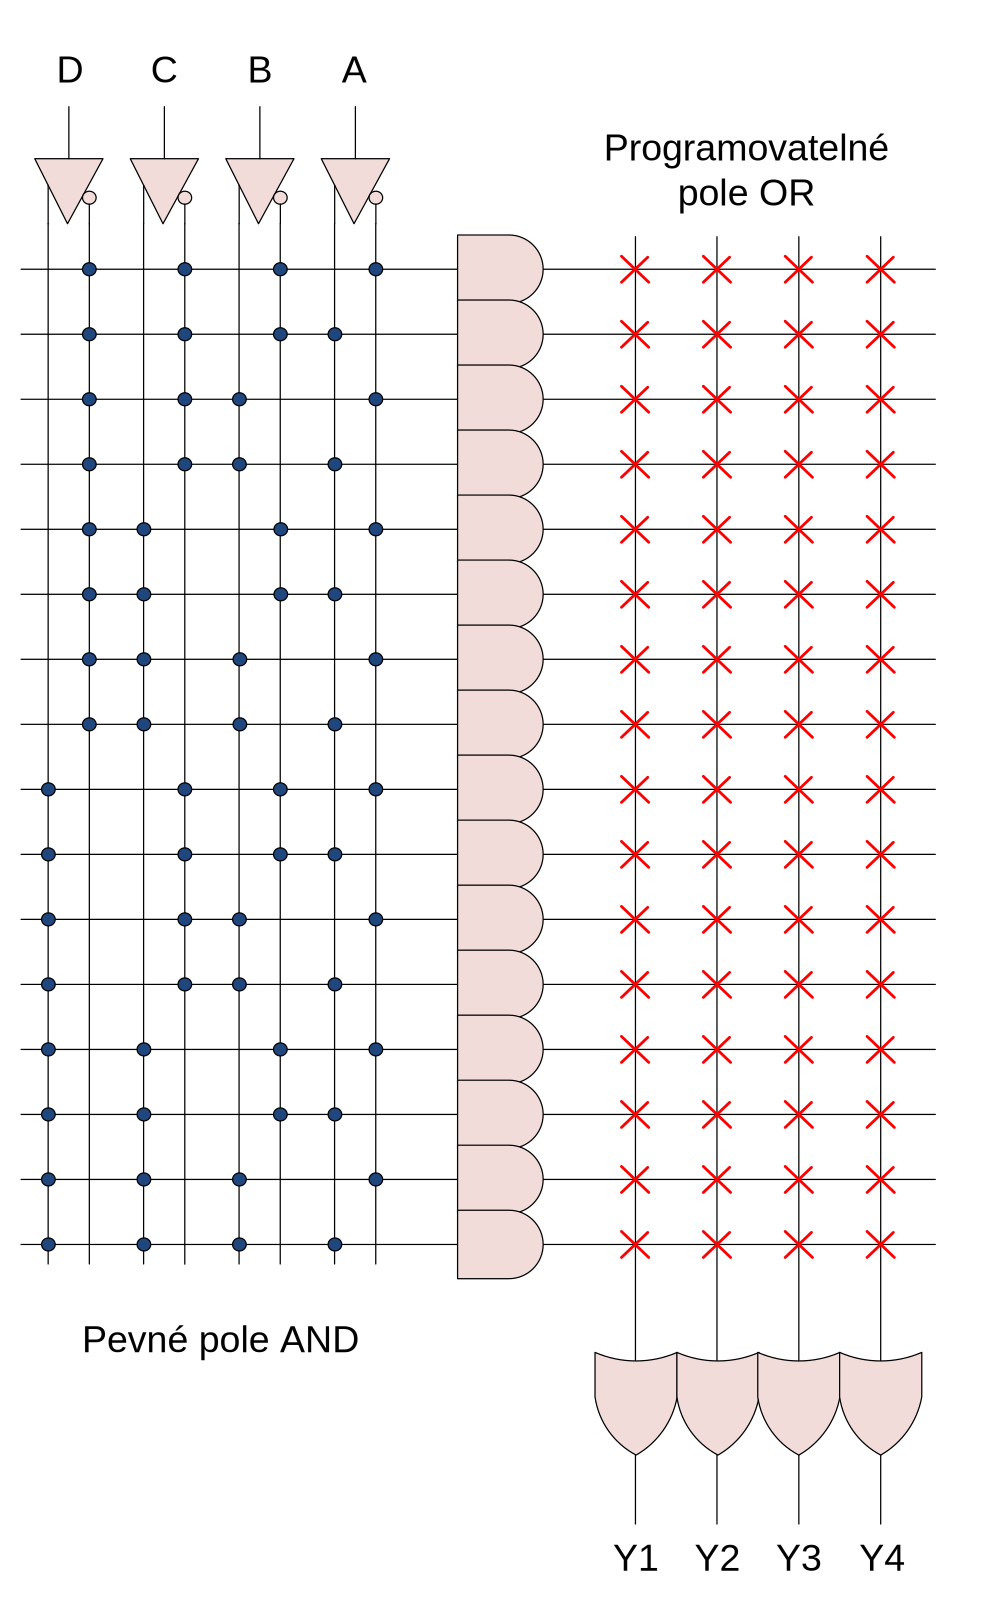
\includegraphics[width=0.8\linewidth]{architektura_PROM.pdf}
          \caption[Architektura PROM]{PLD typu Programmable Read Only Memory (PROM)}
          \label{PLO:fig_arch_PROM}
        \end{figure}
        
        Obvody \texttt{PROM} představuje matici paměťových buněk, jejíž řádky jsou adresovatelné
        vstupní signály a datové sloupce představují výstupní signály. Počet adresových a datových
        signálů determinuje rozměr matice. Např. 4 vstupní signály umožňují adresaci 16 řádků, 4
        datové signály indikují, že každý řádek se skládá ze 4 pamě\-ťo\-vých buněk. Z pohledu
        architektury obvodů PLD obsahují PROM pevné propojovací pole hradel \texttt{AND},
        následované programovatelným polem hradel \texttt{OR} (viz obr. \ref{PLO:fig_arch_PROM})

        \begin{figure}[ht!]
          \centering
          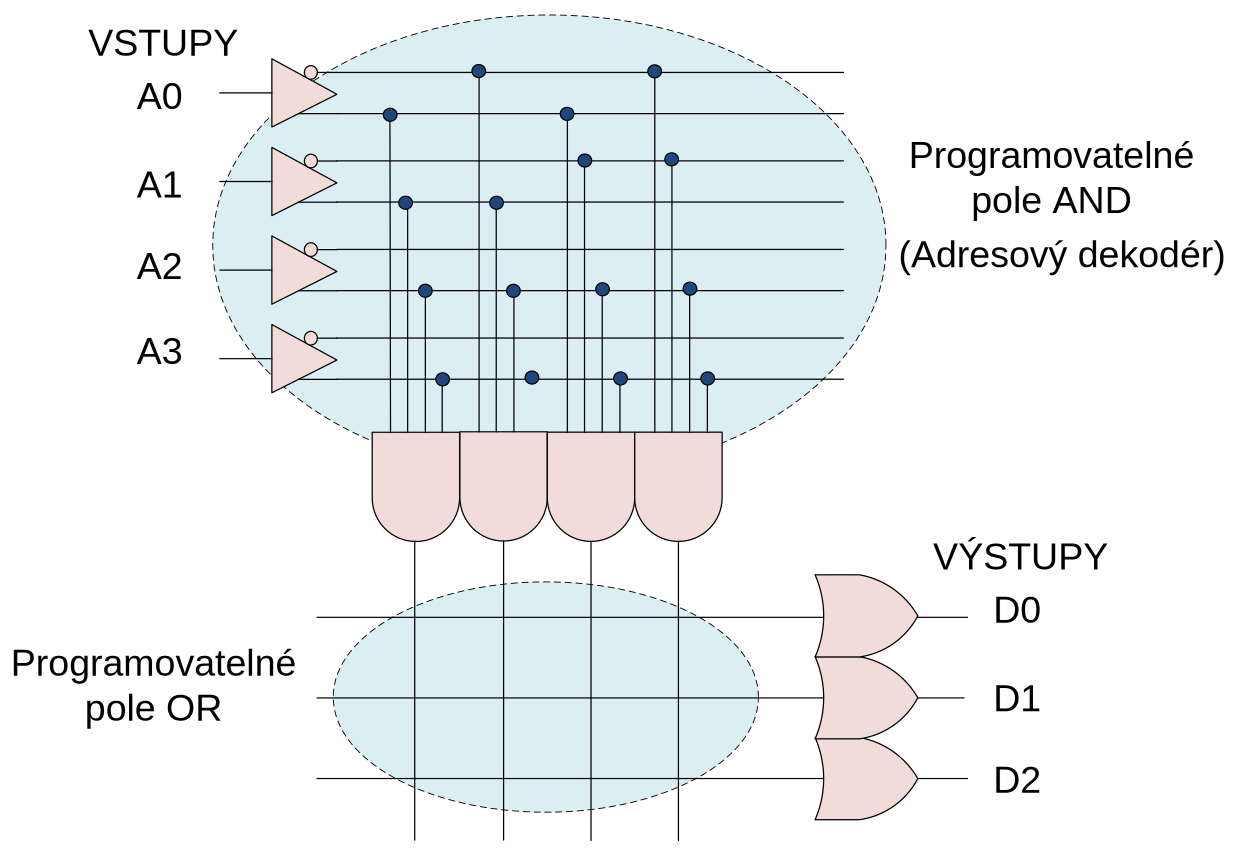
\includegraphics[width=0.9\linewidth]{schema_PROM.pdf}
          \caption[Schéma obvodu PROM]{Schéma obvodu PROM}
          \label{PLO:fig_sch_PROM}
        \end{figure}      

        Všeobecně platí, že obvody PROM jsou nejvhodnějším kandidátem implementace takových
        aplikací, které vyžadují, aby na každou kombinaci vstupních signálů byla jiná odezva
        výstupních signálů. Překážkou je omezení počtu vstupních signálů, eventuálně je limitující
        také velikost programovatelné matice. Její velikost se přidá\-ním nového vstupu vždy
        zdvojnásobí (omezení počtu vstupních signálů jistým způsobem řeší obvody typu PAL viz kap.
        \ref{PLO_kap_PAL})\cite[s.~59]{PLD_Grada}.
      
        Na obr. \ref{PLO:fig_sch_PROM} je uvedena architektura obvodu PROM prostřednictvím
        symboliky obvodů PLD. Každý term odpovídá jedné z jeho adres. Programovatelná hradlo OR
        odpovídají datovým bitům obvodu PROM (výstupní slovo). Např. PROM velikosti 32x8
        představuje obvod PLD s 5 vstupy, 32 součinovými termy ($32=2^5$) a 8 programovatelnými
        výstupními OR hradly.

     \subsubsection{PLD typu Programmable Logic Array (PLA)}\label{PLO_kap_FPLA}
        Obvody \texttt{PLA}(\emph{Programmable Logic Array}) patří k průkopníkům v oblasti
        programovatelných logických polí. Obsahují programovatelné pole hradel AND a zároveň i
        programovatelné pole hradel OR (viz obr. \ref{PLO:fig_arch_FPLA}).
        Vstupní signály jsou přivedeny v přímém i invertovaném stavu do pole AND hradel.
        \begin{figure}[ht!]
          \centering
          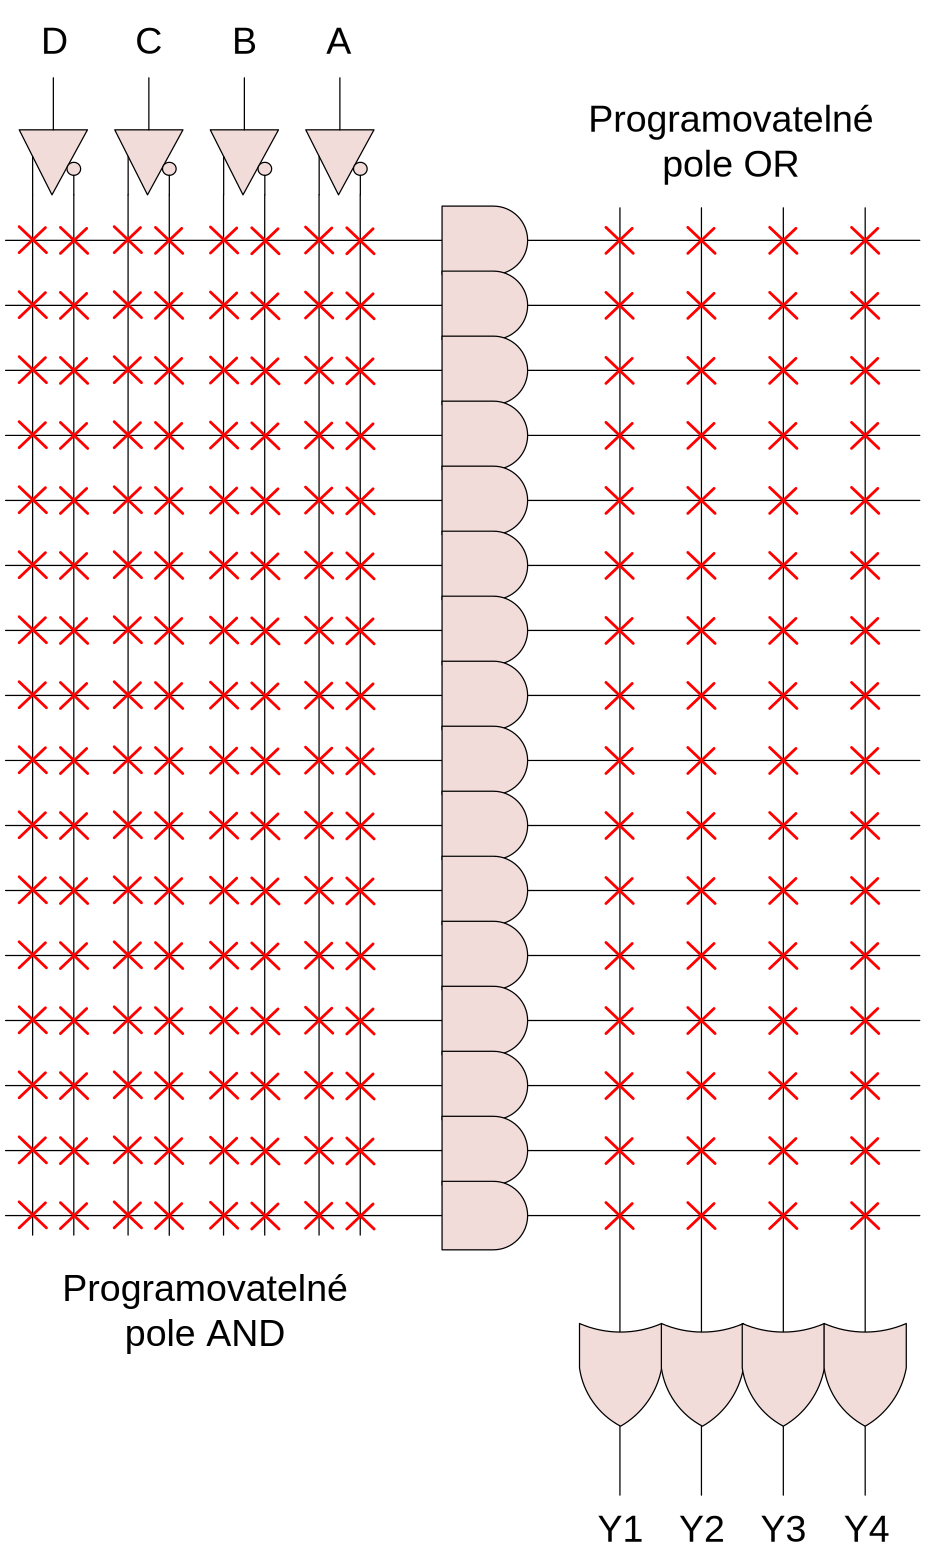
\includegraphics[width=0.8\linewidth]{architektura_FPLA.pdf}
          \caption[Architektura obvodů PLA]{Architektura obvodů PLA}
          \label{PLO:fig_arch_FPLA}
        \end{figure}
        
        Oproti obvodům \texttt{PROM}, mají obvody \texttt{PLA} toto pole programovatelné, takže je
        možné snadno vytvořit součinové termy z libovolné kombinace vstupních (přímých i
        negovaných) signálů. Součinové termy jsou přivedeny do programovatelného pole OR hradel,
        které umožňuje připojení libovolného termu k libovolnému hradlu OR. Jeden term může být
        přiveden na vstup i několika hradel OR. Na jejich výstupu je formována požadovaná logická
        funkce ve tvaru "součtu součinů".

        Je-li obvod PLD vybaven programovatelným polem AND, jako je tomu u obvodů \texttt{PLA} (a i
        např. u PAL kapitola \ref{PLO_kap_PAL}), může být využita pouze polovina programovatelných
        spínačů propojovacího pole. Tato skutečnost je zřejmá, protože vstupní signály jsou do pole
        přivedeny v přímém i invertovaném tvaru a v žádném součin se nemůže současně vyskytovat
        přímý i invertovaný signál (součin by vždy nabýval hodnoty logická nula). Takže nejméně
        polovina (a v praxi i více, protože všechny součiny vždy neobsahují všechny veličiny) není
        při konstrukcích logických funkcí využita. Je tedy zřejmé, jak neefektivně je využita
        plocha křemíkového čipu, na kterém je obvod typu PLA realizován. Tato skutečnost stimuluje
        další vývoj a vznik nových architektur obvodů PLD \cite[s.~63]{PLD_Grada}.
        
     \subsubsection{PLD typu Programmable Array Logic (PAL)}\label{PLO_kap_PAL}
        Obvody typu PAL jsou dalším z typů programovatelných logických obvodů. Jsou to PLD obvody s
        programovatelným polem hradel AND a pevným poler hradel OR. K jednomu hradlu OR lze
        připojit pouze omezený počet součinových termů, přičemž nelze současně jeden term připojit
        k několika hradlům OR.
      
        \begin{figure}[ht!]
          \centering
          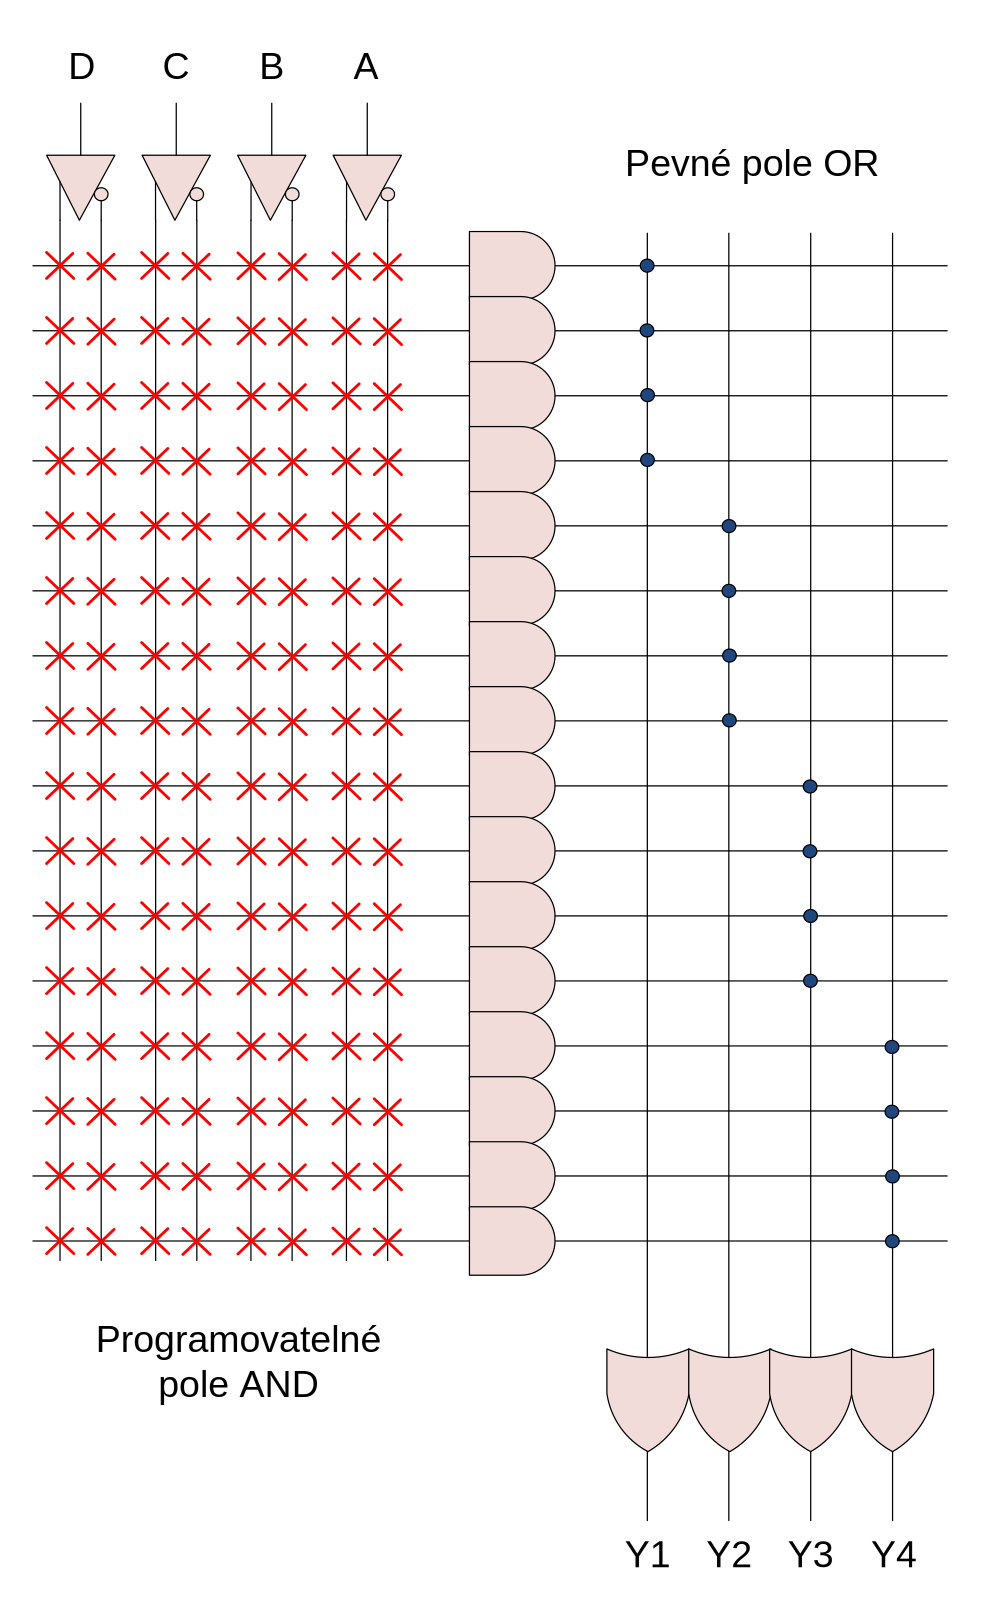
\includegraphics[width=0.8\linewidth]{architektura_PAL.pdf}
          \caption[Architektura obvodů PAL]{Architektura obvodů PAL}
          \label{PLO:fig_arch_PAL}
        \end{figure}
        
        Jednodušší architektura oproti v té době existujícím FPLA obvodům, umožnila zkrácení doby
        přenosu signálu. Obvody PAL byly navrženy tak, aby "vypadaly" jako standardní obvody PROM a
        mohly tak být programovány standardními programátory obvodů PROM. Tím se výrobci obvodů PAL
        vyvarovali požadavků na dodatečné vývojové prostředí, jak tomu bylo v době uvedení na trh v
        případě FPLA obvodů.
        
     \subsubsection{PLD typu Simple Programmable Logic Device - \texttt{SPLD}}\label{PLO_kap_GAL}
       Obvody typu \texttt{GAL} (\emph{Generic Array Logic}) patří do skupiny elektricky
       reprogramovatelých obvodů PLD (\texttt{EEPLD} - \emph{Electrically Erasable Programmable
       Logic Device}). Z hlediska klasifikace PLD obvodů lze obvody \texttt{GAL} charakterizovat
       jako obvody s programovatelným polem AND hradel a pevným polem hradel OR. Významná
       od\-liš\-nost od obvodů PAL spočívá v možnosti elektrického reprogramování a využití
       makro\-buň\-ky (Output Logic Macrocell) na výstupech obvodu.
       
        \begin{figure}[hb!]
          \centering
          \includegraphics[width=0.7\linewidth]{architektura_GAL.pdf}
          \caption[Struktura obvodu GAL]{Obecná struktura obvodu \texttt{GAL}}
          \label{PLO:fig_arch_GAL}
        \end{figure}
               
  \newpage
  \subsection{Obvody typu Complex Programmable Logic Device - \texttt{CPLD}} 
    Obvody typu \texttt{CPLD} patří podobně jako obvody \texttt{SPLD} do skupiny elektricky
    reprogramovatelných \texttt{PLD} obvodů (\texttt{EEPLD}). Většina \texttt{CPLD} obvodů je
    programovatelná v cílovém systému, nesou tedy i označení \texttt{ISP} (\emph{In-system
    programming}). Tyto obvody jsou typické, podobně jako obvody \texttt{GAL}, svou
    programovatelnou maticí hradel AND následovanou hradlem OR a makrobuňkou. Na výstupu hradla OR
    je tak stejně jako u obvodů \texttt{GAL} formována pořadovaná logická funkce ve tvaru
    \emph{součtu součinů}. Od obvodů GAL se však obvody CPLD liší hlavně velkým centrálním
    propojovacím polem. Makrobuňky jsou sdruženy do větších skupin a tvoří tzv. \textbf{funkční
    bloky} \cite[p~279]{Pinker2006}. Pro architekturu obvodů CPLD jsou charakteristické tyto čtyři
    struktury:
    \begin{itemize}
      \item velké centrální propojovací pole (\emph{Global Routing Pool}),
      \item programovatelné funkční bloky  (\emph{Generic Logic Block - GLB}), uspořádané ko\-lem
            propojovacího pole, sestávající z:
        \begin{itemize}
          \item programovatelné matice AND,
          \item několika makrobuňek,
          \item alokátoru součinů,          
        \end{itemize}
      \item výstupní propojovací pole (\emph{Output Routing Pool - ORP}),
      \item vsutpní/výstupní bloky  (\emph{I/O Blocks}).  
    \end{itemize}

        \begin{figure}[hb!]
          \centering
          \includegraphics[width=0.9\linewidth]{PLD_ispMACH4000_arch.pdf}
          \caption{Architektura \texttt{CPLD ispMACH4000} společnosti \texttt{Lattice}}
          \label{PLO:fig_arch_ispMACH4000}
        \end{figure}  
            
    Všechny výše uvedené stavební prkvy mají u různých výrobců různá označení, jejich význam a
    funkce je však velmi podobná. Pomocí makrobuňek lze realizovat různě složité kombinační a
    sekvenční logické či paměťové funkce. Přes programovatelné \textbf{vstupní/výstupní bloky} lze
    přivádět vstupní signály z vývodů obvodu nebo naopak vyvádě výstupní signály. Na rozdíl od
    jednodušších SPLD, kde vstupní/výstupní obvody jsou přímo spojeny s makrobuňkou, jsou však u
    CPLD zásadně od makrobuňek odděleny a tvoří samostatný I/O blok, do kterého mohou výstupní
    signály z makrobuňek vstupovat přes programovatelné \textbf{výstupní propojovací pole}. Tím se
    všeobecně zlepší využití jak makrobuňek, tak výstupních obvodů.
    
    Všechny vstupní/výstupní bloky a všechny makrobuňky lze spolu vzájemně propojit pomocí
    \textbf{centrálního programovatelného propojovacího pole}.

        \begin{figure}[ht!]
          \centering
          \includegraphics[width=0.6\linewidth]{architektura_CPLD.pdf}
          \caption[Struktura obvodu CPLD]{Obecná struktura obvodu CPLD}
          \label{PLO:fig_arch_CPLD}
        \end{figure} 
           
  \subsection{Obvody typu Field-Programmable Gate Array - \texttt{FPGA}}   
    \subsection{Terminologie}
      \begin{itemize}
        \item \textbf{PLA} — \emph{Programmable Logic Array} nebo také \textbf{FPLA} \emph{Field
              Programmable Logic Array}: Obvod obsahuje matici \texttt{AND} za nímž následuje matice
              \texttt{OR}, jež jsou obě programovatelné.
              % is a relatively small FPD that contains two levels of logic, an AND-plane and an
              % OR-plane, where both levels are programmable (note: although PLA structures are
              % sometimes embedded into full-custom chips, we refer here only to those PLAs that are
              % provided as separate integrated circuits and are user-programmable).
        \item \textbf{PAL} - \emph{Programmable Array Logic}\footnote{obchodní známka je v
              současnosti ve vlastnictví společnosti Lattice Semiconductor}: Relativně jednoduchý
              PLD obvod obsahující programovatelnou matici \texttt{AND}, za níž následuje pevná
              matici \texttt{OR} (obr.\ref{PLO:fig_arch_PAL}). %relatively small FPD that has a
              % programmable AND-plane followed by a fixed OR-plane
        \item \textbf{SPLD} — \emph{Simple programmable logic device}: Označení je společné pro   
              \texttt{PLA} a \texttt{PAL} struktury.
              %refers to any type of Simple PLD, usually either a PLA or PAL
        \item \textbf{CPLD} — \emph{Complex programmable logic device}: Název zahrnuje obvody   
              jejichž složitost je někde mezi architekturami obvodů PAL a FPGA a nese rysy obou 
              těchto architektur. Základním stavebním blokem je tzv. \emph{makrobuňka}, která 
              realizuje logický výraz ve tvaru normální disjunktivní formy.   
              %A complex programmable logic device (CPLD) is a programmable logic device with 
              %complexity between that of PALs and FPGAs, and architectural features of both. The 
              %building block of a CPLD is the macrocell, which contains logic
              %implementing disjunctive normal form expressions and more specialized logic 
              %operations. [wiki] ;a more Complex PLD that consists of an arrangement of multiple 
              %SPLD-like blocks on a single chip. Alternative names (that will not be used in this 
              %paper) sometimes adopted for this style of chip are Enhanced PLD (EPLD), Super PAL, 
              %Mega PAL, and others.
        \item \textbf{FPGA} — \emph{Field-Programmable Gate Array}: Obvody mají z 
              programovatelných obvodů nejobecnější strukturu  a obsahují nejvíce logiky. Základním 
              stavebním blokem jsou logické buňky (\emph{\emph{logic elements}}; Altera), nebo   
              také řezy (\emph{slices}; Xilinx), jež jsou zpravidla sdruženy do větších logických 
              bloků\footnote{Výrobci FPGA obvodů používají vlastní názvosloví k popisu jejich 
              architektur.} (\emph{logic array block}, \texttt{LAB}; Altera) resp.          
              (\emph{configurable logic block}, \texttt{CLB}; Xilinx). Logické buňky obsahují tzv. 
              vyhledávací tabulku (\emph{Look-up table}, \texttt{LUT}), která dovoluje realizovat 
              jednoduché kombinační funkce. LUT má obvykle čtyři vstupní signály, které mají význam 
              indexu (pointeru) do této tabulky. K propojení \texttt{CLB} slouží programovatelná 
              propojovací struktura \texttt{PI} (\emph{programmable interconnect}).
              % The main distinction between FPGA and CPLD device architectures is that FPGAs are 
              %internally based on Look-up tables (LUTs) while CPLDs form the logic functions with 
              % sea-of-gates (e.g. sum of products). [wiki];a Field-Programmable Gate Array is an 
              %FPD featuring a general structure that allows very high logic capacity. Whereas 
              %CPLDs feature logic resources with a wide number of inputs (AND planes), FPGAs offer 
              %more narrow logic resources. FPGAs also offer a higher ratio of flip-flops to logic 
              %resources than do CPLDs.
    \end{itemize}

  \section{Dynamické parametry PLD}
     Programovatelné logické obvody mohou pracovat jako obvody kombinační, nebo častěji jako obvody
     sekvenční \cite[p~593]{Wakerly1999}. Symboly pro doby jenž jsou dále popsány, se v různých
     firemních publikací liší, význam však zůstáva.
    \begin{itemize}\addtolength{\itemsep}{-0.5\baselineskip}
      \item $t_{PD}$ - \emph{doba zpoždění} - ve funkci kombinačního obvodu $t_{PD}$ je doba od
            změny signálů na vstupech obvodu do změny signálů na jeho výstupech. Je podstatná pro
            režim bez hodinových impulzů u ryze kombinačního  obvodu. U sekvenčního obvodu
            \emph{Mealyho} typu je to zpoždění obvodu v době mezi hodinovými impulzy,
      \item $t_{CO}$ - \emph{doba zpoždění po hodinovém impulzu} - doba od aktivní hrany hodinového
            impulzu do změny výstupního signálu,
      \item $t_{CF}$ - opět se jedná o zpoždění jako v předchozím případě, tj. je to doba od 
            aktivní hrany hodinového impulzu do změny výstupního signálu registru, jenž je ovšem 
            veden jako zpětnovazební vstup. Běžně platí, že $t_{CF}<t_{CO}$ a pokud
        jej výrobce neuvádí, lze předpokládat $t_{CF}=t_{CO}$
      \item $t_{SU}$- \emph{doba předstihu} - je doba, po kterou vstupní signál musí být 
            konstantní až do aktivní hrany hodinového impulzu,
      \item $t_{H}$ - \emph{doba přesahu} - je doba, po kterou vstupní signál musí být konstantní 
            po aktivní hraně hodinového impulzu,
      \item $f_{max}$ - \emph{maximální kmitočet hodinových impulzů} - Je to nejvyšší frekvence, 
            na které zařízení může pracovat spolehlivě a je ekvivalentní k převrácené hodnotě 
            minimální periody hodinových impulzů.
    \end{itemize}
    
    \begin{figure}[ht!]
      \centering
      \begin{tabular}{c}
        \subfloat[Doba zpoždění $t_{PD}$]{\label{PLO:fig_PLD_timing_tpd}
          \includegraphics[width=0.7\linewidth]{PLD_timing_tpd.pdf}}                     \\
        \subfloat[Doba zpoždění po hodinovém impulzu $t_{CO}$, doba předstihu ]
          {\label{PLO:fig_PLD_timing_tsu}
          \includegraphics[width=0.7\linewidth]{PLD_timing_tsu_th_tco_fmax.pdf}}         \\
        \subfloat[ ]{\label{PLO:fig_PLD_timing_tcf}
        \includegraphics[width=0.7\linewidth]{PLD_timing_tsu_tcf_fmax.pdf}} 
      \end{tabular}             
      \caption{Základní dynamické parametry PLD: $t_{PD}$, $t_{CO}$, $t_{CF}$, $t_{SU}$,
               $t_{H}$, $f_{max}$}
      \label{PLO:fig_PLD_timing}
    \end{figure}  
        
     Dynamické parametry u programovatelných logických obvodů jsou závislé na vnitř\-ních cestách 
     signálů. U obvodů \texttt{CPLD} je situace jednodušší, neboť cesty signálů jsou do jisté míry 
     pevně dány a jedná se jen o jejich výběr. Výrobci uvádějí korekční vztahy pro výše uvedené 
     doby, kterými jsou respektovány logické zátěže a způsob využití vnitřních bloků. Složitější
     situace je u obvodů \texttt{FPGA}, kde cesty signálů nejsou předem definovány a v procesu 
     návrhu budou teprve vyvtářeny. Jednotlivé doby proto musí dodatečně dopočítat návrhový systém 
     \cite[p~288]{Pinker2006}.

} % tikzset
%---------------------------------------------------------------------------------------------------
\printbibliography[title={Seznam literatury}, heading=subbibliography]
\addcontentsline{toc}{section}{Seznam literatury}
%  % !TeX spellcheck = cs_CZ
{\tikzset{external/prefix={tikz/CES/}}
 \tikzset{external/figure name/.add={ch11_}{}}
%---------------------------------------------------------------------------------------------------
% file VHDL.tex
%---------------------------------------------------------------------------------------------------
\lstset{ %
  language=VHDL,                         % choose the language of the code
  basicstyle=\small,                     % the size of the fonts that are used for the code: 
                                         % basicstyle=\small, \footnotesize
  backgroundcolor=\color{White},         % choose the background color. You must add  
                                         % \usepackage{color}
  commentstyle=\color{help}\textit,
  stringstyle=\ttfamily,                 % typewriter type for strings
  keywordstyle=\color{keyword}\textbf,
  breaklines=true,                       % sets automatic line breaking
  breakatwhitespace=true,                % sets if automatic breaks should only happen at whitespace
  showspaces=false,                      % show spaces adding particular underscores
  showstringspaces=true,                 % underline spaces within strings
  showtabs=true,                         % show tabs within strings adding particular underscores
  frame=none,	                           % adds a frame around the code - none, single
  tabsize=8,                             % sets default tabsize to 8 spaces
  captionpos=b,                          % sets the caption-position to bottom
  numbers=left,                          % where to put the line-numbers -none, left, right
  numberstyle=\footnotesize,             % the size of the fonts that are used for the line-numbers
  stepnumber=1,                          % the step between two line-numbers. If it's 1 each line
                                         % will be numbered
  xleftmargin=3em,                       % adjust left margin
}
%===========================Kapitola: Jazyk VHDL==================================================
\chapter{Jazyk VHDL}
\minitoc

  \section{Návrh číslicového obvodu}
    \subsection{Popis číslicové funkce}
      Máme-li představu o funkci a struktuře budoucího číslicového obvodu, nastupuje proces 
      \emph{zachycení návrhu} (design entry, design capture), při kterém je nutné naše představy 
      přenést do počítačem zpracovatelné formy. Tuto úlohu, lze splnit na různých úrovních 
      abstrakce \cite[s.~19]{Stastny2010}:
      \begin{itemize}
        \item \textbf{hradlové/schématické} - navrhujeme přímo kreslením schématu budoucího 
              obvodu. Výhodou tohoto postupu je jeho srozumitelnost a zachycení skuteč\-né podoby 
              návrhu  - co máme ve schématu je to, co se realizuje. Nevýhody nicméně převyšují 
              výhody. Kreslení schéma je obvykle specifické pro zvolený obvodu, protože často 
              používáme struktury, které jsou k dispozici jen na příslušném PLD obvodu. Konverze do 
              jiného obvou, znamená překreslení schématu. Vlastní proces kreslení je pomalý a 
              únavný, protože pracujeme na nízké úrovni abstrakce - kreslíme obvod hradldo po 
              hradle. Chceme-li například realizovat stavový automat, musíme nejprve zminimalizovat 
              jeho přechodovou a výstupní funkci a pak nakreslit schéma. Snadno se můžeme dostat do 
              situace, kdy je nutné kompletní překreslení. 
        \item \textbf{meziregistrových přenosů} - tzv. \texttt{RTL} (\emph{Register Transfer  s  
              Level}). \texttt{RTL} popis je dnes standardním prostřekdem pro popis číslicové 
              funkce. Číslicové synchronní obvody se skládají ze dvou základních typů         
              logických bloků: pamě\-ťo\-vých prvků (registrů) a kombinačních funkcí. Na úrovni 
              abstrakce, číslicový obvod popisujeme tak, že jednotlivé struktury popíšeme pomocí 
              těchto dvou typů logiky a doplníme informací o jejich vzájemném propojení          
              (odkud, kam a přes jaké kombinační logické funkce jsou přelévána data mezi registry). 
              Popis obvodu je realizován v textové podobě pomocí zápisu ve speciálním 
              progra\-mo\-va\-cím jazyku (\texttt{HDL} - \emph{Hardware Description         
              Language}). Pro popis se používají nejčastěji jazyk \texttt{VHDL} a \texttt{Verilog}. 
              Použití \texttt{RTL} úrovně má nesporné výhody: získáme technologicky nezávislý popis 
              obvodu na relativně vysoké úrovni abstrakce, přičemž jeden řádek zdrojového kódu je v 
              hardware reprezentován typicky desítkami/stovkami hradel. To zvyšuje produktivitu 
              práce, zpřehledňuje vlastní návrh, zjednodušuje přenos návrhu mezi různými 
              technologiemi a zrychluje jak vlastní návrh, tak pozdější opravy. Jedinou 
              nevý\-ho\-dou je nevhodnost pro ryze asynchronní návrh, to ale není při práci s     
              hrad\-lo\-vý\-mi poli omezující, neboť hradlová pole jsou určena právě pro synchronní 
              číslicové obvody.
        \item \textbf{algoritmické} - neustále se zkracující délka návrhového cyklu spolu s  
              rostoucí komplexitou navrhovaných systémů nutí návrháře používat stále vyšší úrovně 
              abstrakce. Architektura na \texttt{RTL} úrovni je navrhována vždy s ohledem ke 
              skutečnému časování obvodu a použitém paralelizmu. Systém je na této úrovni narvržen 
              s odpovídajícím počtem výpočetních jednotek, řídicích bloků, sběrnic, apod. Problém 
              nastává v okamžiku, kdy v pozdějších fázích návrhu zjistíme, že navržená architektura 
              nesplňuje očekávání. Právě od\-stra\-ně\-ní informace o paralelismu a časování ze 
              zdrojového kódu je přínosem \emph{algoritmické syntézy}. Funkce bloku je popsána v 
              některém z jazyků na ''vyšší úrovni'' - např. \texttt{ANSI C}, \texttt{Handel-C}, 
              \texttt{SystemC}, nebo \texttt{System Verilogu}. Příslušný syntézní nástroj pak    
              dostane informaci o počtu funkčních jednotek a časování ve formě jednoduchých oemzení 
              (například povolíme použití nejvýše dvou násobiček a dvou sčítaček) a na základě 
              pžedloženého algoritmu vygeneruje \texttt{RTL} kód výsledného systému (datových cest 
              i řídicích bloků). Kaž\-dá změna v architektuře je triviální - zjistíme-li, že 
              výpočetní výkon systému je příliš nízký, stačí jen znovu spustit syntézní proces s 
              jiným počtem aritmetických jednotek. Rychlost celého procesu umožňuje vyzkoušet celou 
              řadu alternativ architektury a najít nejvhodnější kompromis mezi plochou a rychlostí 
              obvodu. Zjednodušuje se i verifikace. Použitelnost algoritmické syntézy zatím omezuje 
              fakt, že výsledek není tak dobrý v porovnání s návrhem od profesionála. 
      \end{itemize}
  \section{Úvod}
    Název VHDL představuje akronym — \texttt{VHSIC} \texttt{Hardware Des\-cription Language}. Samo 
    označení \texttt{VHSIC} je další akronym představující název projektu, v rámci něhož byl jazyk 
    VHDL zpracován, a znamená \texttt{Very High Speed Integrated Circuits}. I když označení 
    \texttt{VHDL} v tomto kontextu není příliš přiléhavé, vžilo se a obecně se používá. Jazyk VHDL 
    byl původně vyvinut především pro modelování a simulaci rozsáhlých systémů. Na mnoha jeho 
    konstruktech je to znát, některé z nich nemají pro syntézu vůbec význam. Zde se však budeme 
    zabývat především použitím jazyka VHDL k vytváření modelů určených pro syntézu číslicových 
    systémů. České termíny budou v prvním výskytu zapsány tučně. Často tyto termíny nejsou 
    ustálené, a proto budeme uvádět i jejich anglické ekvivalenty, které již většinou mají 
    ustálenou podobu.

  % ------------- Základní vlastnosti jazyka VHDL --------------------------------------------------
  \section{Základní vlastnosti jazyka VHDL}
     \begin{itemize}
       \item Je to otevřený standard (\emph{open standard}). K jeho použití pro sestavení  
             návrhových systémů není třeba licence jeho vlastníka, jako je tomu u jiných jazyků HDL 
             (například u jazyka \texttt{ABEL}). To je jeden z důvodů, proč je tento jazyk v 
             návrhových systémech často používán.
       \item Umožňuje pracovat na návrhu, aniž je předtím zvolen cílový obvod. Ten může být zvolen 
             až v okamžiku, kdy jsou známy definitivní požadavky na prostředí, v němž má navrhovaný 
             systém pracovat, a je možno cílový obvod měnit podle potřeby při zachování textu 
             popisujícího systém, může být zvolen obvod \texttt{PLD} nebo \texttt{FPGA} 
             (\emph{Device-independent design}).
       \item Je možno provést simulaci navrženého obvodu na základě téhož zdrojového textu, 
             který pak bude použit pro syntézu a implementaci v cílovém obvodu. Zdrojový text je 
             možno zpracovávat v různých simulátorech a v syntetizérech různých výrobců. 
             Odsimulovaný text může být použit v dalších projektech s různými cílovými obvody, což 
             je podporováno hierarchickou strukturou jazyka. Této vlastnosti jazyka se říká 
             přenositelnost (\emph{portability}) kódu.
       \item V případě úspěšného zavedení výrobku na trh lze popis modelu systému v jazyku VHDL   
             použít jako podklad pro jeho implementaci do obvodů \texttt{\textbf{ASIC}} vhodných 
             pro velké série.
     \end{itemize}
     \textbf{Některé námitky proti VHDL:}
     \begin{itemize}
       \item Jazyk VHDL je dosti „upovídaný", jazykové konstrukty nejsou navrženy tak, aby 
             zdrojový text byl stručný a při popisu modelu určitého systému se setkáme s 
             opakováním bloků stejného znění. Ty je však možno snadno vytvářet využitím        
             kopírování a podobných možností současných editorů.
       \item V jazyku VHDL je možno vytvořit neefektivní konstrukce, efektivnost nebo její   
             nedostatek nemusí být na první pohled ze zdrojového textu patrné. To je však vlastnost 
             i jiných jazyků vyšší úrovně a výsledná efektivnost konstrukce závisí nejen na kvalitě 
             programových návrhových prostředků, ale také na zkušenosti konstruktéra (návrháře).
     \end{itemize}
  
    Základní verze jazyka VHDL byla přijata jako standard \texttt{IEEE} číslo 1076 v roce 1987. 
    Konstrukty odpovídající tomuto standardu se označují jako konstrukty jazyka \texttt{VHDL-87}. 
    Podobně jako další standardy \texttt{IEEE}, i tento standard se v pravidelném pětiletém 
    intervalu aktualizuje. Upravená verze standardu byla přijata v roce 1993, odkazuje se na ni jako
    na standard \texttt{VHDL-93}.
  
    Vedle jazyka \texttt{VHDL} se setkáme také s jazykem \texttt{Verilog}, který má podobné 
    použití. Uvádí se, že jazyk \texttt{VHDL} je rozšířený zejména v Evropě, zatímco 
    \texttt{Verilog} se používá hlavně v asijských zemích. V USA se používají oba tyto jazyky.
    
    Vyjadřovací schopnosti jazyku VHDL jsou dány příkazy, jenž mají souběžný nebo sekvenční 
    charakter. Některé příkazy jsou jen jednoho druhu, jiné mohou být obojího druhu. Toto rozlišení 
    se týká toho, ve které části popisu se příkazy mohou používat. Pro stručnost budeme dále mluvit 
    o souběžných a o sekvenčních příkazech, i když jde spíše o to, kde se tyto příkazy nacházejí
    či mohou nacházet. V následujících kapitolách jsou příkazy rozděleny do dvou velkých skupin: 
       \begin{itemize}
         \item \hyperref[Section:VHDL_soubezne_prikazy]{Souběžné příkazy} (\emph{concurrent  
               statements}): zapisují se v textu jazyka mimo procesy, definice funkcí a procedur.
         \item \hyperref[Section:VHDL_sekvencni_prikazy]{Sekvenční příkazy} (\emph{sequential  
               statements}): slouží k algoritmickému vyjádření popisu. Tyto příkazy mohou být 
               zapsány jen v procesech, v definicích funkcí a procedur.
       \end{itemize}
  % ------------------------------------------------------------------------------------------------------------------------------
  \section{Logické úrovně}
   Od jazyka určeného k návrhu a modelování integrovaných obvodů očekáváme schopnost modelovat 
   základní logické úrovně - \emph{log. 0} a \emph{log. 1}. Ty jsou pro jednoduché simulace 
   postačující, ale již například pro návrh a modelování třístavových budičů sběrnic potřebujeme 
   mít možnost pracovat se stavem vysoké impedance \emph{Z}. Dalším jednoduchým příkladem může byt 
   modelování zkratu na sběrnici, který může vzniknout v situaci, kdy dva budiče budí jeden spoj
   opačnými logickými úrovněmi. Balíček \texttt{std\_logic\_1164} knihovny \texttt{IEEE} pro tyto 
   účely zavádí \emph{devítistavovou logiku}. 
   
   \begin{itemize}\addtolength{\itemsep}{-0.5\baselineskip}
     \item 'U': uninitialized. This signal hasn't been set yet.
     \item 'X': unknown. Impossible to determine this value/result.
     \item '0': logic 0
     \item '1': logic 1
     \item 'Z': High Impedance
     \item 'W': Weak signal, can't tell if it should be 0 or 1.
     \item 'L': Weak signal that should probably go to 0
     \item 'H': Weak signal that should probably go to 1
     \item '-': Don't care.
   \end{itemize}
   
   Všimněme si, že tato knihovna je připojena všemi ukázkovými kódy. Logický signál, který má 
   popsaných hodnot nabývat, je pak definován jako signál typu \texttt{std\_logic}, nebo 
   \texttt{std\_logic\_vector} pokud se jedná o sběrnici. Pomocí nich modelujeme standardní 
   propojení logických prvků, tj. ''obyčený kus drátu''.
   \cite[s.~51]{Stastny2010}
  \section{Souběžné příkazy} \label{Section:VHDL_soubezne_prikazy}
  \newpage
  \section{Sekvenční příkazy}\label{Section:VHDL_sekvencni_prikazy} 
  \section{Technologicky nezávislá část návrhu}
    V následujícím textu jsou uvedeny základní způsoby popisu chování sekvenčních (např. klopné 
    obvody) a kombinačních obvodů. Klopné obvody jsou rozdělovány na \textbf{hranově citlivé} a 
    \textbf{úrovňově citlivé}. Je možné je popsat jako \emph{jednobitové paměti}. Hranově citlivý 
    klopný obvod je obvod řízený změnou na vstupu synchronizace (\emph{clock input}).
    Bývá označován "\emph{flip-flop}".  Úrovňově citlivý klopný obvod je nazýván v české 
    terminologii \emph{zdrž}. Obvykle je však srozumitelný anglický název "\emph{latch}".
  
    \subsection{Dynamicky řízené sekvenční obvody}
      Obvody řízené změnou signálu na vstupu synchronizace jsou ve VHDL popisovány použitím příkazu 
      process a podmíněného příkazu  \lstinline[basicstyle=\ttfamily]!if!. V podmíně\-ném příkazu 
      jsou rozlišovány události (\lstinline[basicstyle=\ttfamily]!events!), které znamenají 
      vzestupnou hranu nebo sestupnou hranu signálu na vstupu synchronizace. Při popisu je možné 
      použít dvou různých zápisů, ve kterých se objevuje atribut události synchronizačního
      signálu \lstinline[basicstyle=\ttfamily]!clk clk'event! nebo volání funkce.
      \begin{itemize}\addtolength{\itemsep}{-0.5\baselineskip}
        \item \lstinline[basicstyle=\ttfamily]!(clk'event and clk='1')!  	 vzestupná hrana signálu
        \item \lstinline[basicstyle=\ttfamily]!(clk'event and clk='0')!    sestupná hrana signálu
        \item \lstinline[basicstyle=\ttfamily]!rising_edge(clk)!		     voláni funkce vzestupné hrany
        \item \lstinline[basicstyle=\ttfamily]!falling_edge(clk)!		     voláni funkce sestupné hrany
      \end{itemize}
      Uvedené příklady ukazují možnosti vyjádření vzestupné a sestupné hrany ve VHDL. Vyjádření 
      pomocí atributu je častěji používané, protože tento konstrukt je rozeznatelný při syntéze 
      obvodového řešení. Nicméně použití volání funkce je výhodnější při simulaci, protože nastává 
      pouze při změně signálu \lstinline[basicstyle=\ttfamily]!clk! z $0\rightarrow1$ a
      z $1\rightarrow0$, ale ne z $X\rightarrow1$ nebo z $0\rightarrow X$, které nepředstavují 
      platný přechod z jednoho stavu do druhého. Devět hodnot signálu, které jsou označované jako 
      \lstinline[basicstyle=\ttfamily]!std_logic! jsou určeny k modelování poruchových stavů 
      logické sítě. Jsou to hodnoty \emph{'U','X','0','1'¸'Z','W','L','H','-'}.
 
        \subsection{Staticky řízené sekvenční obvody}
          V následujících odstavcích jsou popisovány klopné obvody řízené úrovní synchronizačního signálu, které jsou známé pod
          názvem \textbf{zdrž} (\emph{latch}).
    
    \subsection{Kombinační obvody} 

  \section{Knihovna LPM}
    Knihovna \textbf{LPM} (angl. \emph{Library of Parametrized module}) obsahuje parametrizovatelné 
    moduly jako jsou hrada, čítače, multiplexory, klopné obvody, aritmetické a paměťové funkce. 
  
    Standard \texttt{LPM} byl navržen v roce 1990 jako jedna z monžností pro efektivní návrh 
    číslicových systémů do odlišných technologií, jako jsou např. obvody PLD, hradlová pole a 
    standardní buňky. Předběžná verze standardu vyšla v roce 1991, další úprava předběžné verze pak 
    v roce 1992. Standard byl přijat organizací \texttt{EIA} (angl. \emph{Electronic Industires 
    Alliance}) v dubnu roku 1993 jako doplněk do standardu \texttt{EDIF}.
  
    \texttt{EDIF} je formát pro přenos návrhu mezi návrhovými nástroji různých výrobců. Formát 
    \texttt{EDIF} popisuje syntaxi, která reprezentuje logický netlist. \texttt{LPM} do něj pak 
    přidává množinu funkcí, která popisuje logické operace netlistu. Před rozšířením o \texttt{LPM} 
    musel každý \texttt{EDIF} netlit typicky obsahovat technologicky specifické logické funkce,
    které zabraňovaly tomu, aby byl návrh ve větší míře nezávislý na cílové technologii \cite[s.~72]{Pinker2006}. 
  
    \subsection{Posuvný registr - lpm shiftreg}
  
    \begin{table*} 
      \centering
      \begin{tabular}{|c|p{3.5cm}|p{8cm}|}
        \hline
           \rowcolor{CornflowerBlue} {\textbf{Jméno}} & {\textbf{Popis}} & {\textbf{komentář}} \\
        \hline\hline       
           \texttt{data[]}   & Data input to the shift register    
                             & Šířku registru určuje parametr \texttt{LPM\_WIDTH}. \\
        \hline   
           \texttt{clock}    & Positive-edge-triggered clok        
                             & Vstup hodinového signálu. \\
        \hline     
           \texttt{enable}   & Clock enable input                  
                             & Blokuje hodinový signál. \\
        \hline      
           \texttt{shiftin}  & Serial shift data input             
                             & Pro funkci je nutné použit alespoň jeden ze signálů
                               \texttt{data[]}, \texttt{aset}, \texttt{aclr}, \texttt{sset}, 
                               \texttt{sclr}, a/nebo \texttt{shiftin}.  \\
        \hline    
           \texttt{load}     & Synchronous parallel load           
                             & (1) load operation (podmínka: \texttt{enable} = 1); (0) shift
                               operation (výchozí). \\
        \hline    
           \texttt{aclr}     & Asynchronnous clear input          
                             & Signál \texttt{aclr} má vyšší prioritu než signál
           \texttt{aset}.  \\
        \hline    
           \texttt{aset}     & Asynchronnous set input             
                             & Naplní registr \texttt{g[]} hodnotou \texttt{LPM\_AVALUE} \\
        \hline 
           \texttt{sclr}     & Synchronous clear input             
                             & Signál \texttt{sclr} má vyšší prioritu než signál
           \texttt{sset}.  \\
        \hline  
           \texttt{sset}     & Syncrhonous set input              
                             & Naplní registr \texttt{g[]} hodnotou \texttt{LPM\_SVALUE} \\
        \hline  
           \texttt{q[]}      & Data output from the shift register 
                             & Šířku registru určuje parametr \texttt{LPM\_WIDTH}. Vyžaduje
           \texttt{shiftout}.  \\
        \hline 
           \texttt{shiftout} & Serial shift data output          
                             & Vyžaduje registr \texttt{q[]}. \\
        \hline                                                           
      \end{tabular}
      \caption{Popis portů komponenty \texttt{lpm\_shiftreg}.}
      \label{VHDL:tab_lpm_shiftreg}       
    \end{table*}
    
    %---------------------------------------------------------------
    \lstinputlisting{../src/CES/VHDL/lpm_shiftreg.vhd}
    %---------------------------------------------------------------

} % tikzset
%---------------------------------------------------------------------------------------------------
\printbibliography[title={Seznam literatury}, heading=subbibliography]
\addcontentsline{toc}{section}{Seznam literatury} 
}
{
% DEBUG was off
%======================= Kapitola01: ANSI C pro  mikrokontroléry ===================================
  % !TeX spellcheck = cs_CZ
{\tikzset{external/prefix={tikz/CES/}}
 \tikzset{external/figure name/.add={ch05_}{}}
%---------------------------------------------------------------------------------------------------
% file ANSI_C_MCU.tex
%---------------------------------------------------------------------------------------------------
%============================= Kapitola: Stručný úvod===============================================
\lstset{ %
  language=C,                            % choose the language of the code
  basicstyle=\footnotesize\ttfamily,     % the size of the fonts that are used for the code
  backgroundcolor=\color{White},         % choose the background color. 
  commentstyle=\color{help}\textit,
  keywordstyle=\color{blue}\textbf,
  breaklines=true,                       % sets automatic line breaking
  breakatwhitespace=true,                % sets if automatic breaks should only happen at whitespace
  showspaces=false,                      % show spaces adding particular underscores
  showstringspaces=true,                 % underline spaces within strings
  showtabs=true,                         % show tabs within strings adding particular underscores
  frame=none,	                           % adds a frame around the code - none, single
  tabsize=8,                             % sets default tabsize to 8 spaces
  captionpos=b,                          % sets the caption-position to bottom
  numbers=left,                          % where to put the line-numbers -none, left, right
  numberstyle=\footnotesize,             % the size of the fonts that are used for the line-numbers
  stepnumber=1,                          % the step between two line-numbers. If it's 1 each line
  % will be numbered
  xleftmargin=3em,                       % adjust left margin
}

\chapter{ANSI-C pro mikrokontroléry}
\minitoc

  %============= Podkapitola: Preprocesor jazyka C =================================================
  \section{Preprocesor jazyka C}
    Preprocesor interpretuje jednoduché direktivy pro vložení zdrojového kódu z jiného souboru 
    (\lstinline[basicstyle=\ttfamily]!#include!), definice maker 
    (\lstinline[basicstyle=\ttfamily]!#define!) a podmíněné vložení kódu 
    (\lstinline[basicstyle=\ttfamily]!#if!). \texttt{C} preprocesor přijímá tyto direktivy:
    
    \begin{table}[ht!]
      \centering
      \begin{tabular}{c c c c}
        \hline
        \lstinline[basicstyle=\ttfamily]!#define!  & \lstinline[basicstyle=\ttfamily]!#elif! & 
        \lstinline[basicstyle=\ttfamily]!#else!    & \lstinline[basicstyle=\ttfamily]!#endif! \\
        \lstinline[basicstyle=\ttfamily]!#error!   & \lstinline[basicstyle=\ttfamily]!#if! & 
        \lstinline[basicstyle=\ttfamily]!#ifdef!   & \lstinline[basicstyle=\ttfamily]!#ifndef! \\
        \lstinline[basicstyle=\ttfamily]!#include! & \lstinline[basicstyle=\ttfamily]!#line! & 
        \lstinline[basicstyle=\ttfamily]!#pragma!  & \lstinline[basicstyle=\ttfamily]!#undef! \\
        \hline            
      \end{tabular}
      \caption{Seznam platných direktiv jazyka \texttt{C}}\label{S4101C1:C_tab_direktiva}
    \end{table} 
    
    \subsection{Připojení externích souborů}
    
    \subsection{Definice maker}
      Definice maker ve významu rozsahů polí je typickým příkladem použití preprocesoru. Ve 
      zdrojovém textu se neodvoláváme na magická čísla, ale na vhodně symbolicky pojmenovaná makra, 
      která zvýší čitelnost programu.
      
      Pro větší přehlednost rozdělme makra na 
      \begin{itemize}
       \item symbolické konstanty,
       \item makra
      \end{itemize}
      Klíčem nechť je skutečnost, že makro na rozdíl od symbolické konstanty má argumenty.
      \subsection{Symbolické konstanty}
      \subsection{Makra}   
     
    \subsection{Podmíněný překlad}  
      Preprocesor může během své činnosti vyhodnocovat, je-li nějaké makro definováno, či nikoliv. 
      Při použití klíčového slova preprocesoru \texttt{defined} pak může spojovat taková 
      vyhodnocení do rozsáhlejších logických výrazů. Argument defined nemusí být uzavřen do 
      závorek. Může se však vyskytnout jen za \lstinline[basicstyle=\ttfamily]!#if! nebo 
      \lstinline[basicstyle=\ttfamily]!#elif!. Například si ukažme složitější podmínku:

  \section{Pointery}
    \textbf{Pointery} (též ukazatele nebo směrníky) jsou \emph{"srdce a duše jazyka C"}. Pointer je 
    proměnná, jako každá jiná, pouze hodnota uložená v této proměnné má jiný význam. Pointer 
    představuje \textit{adresu paměti} a na této adrese se teprve ukrývá příslušná hodnota. Pointer 
    je tedy proměnná uchovávající paměťovou adresu.\cite{Herout}
  
    \subsection{Práce s pointery}
      \begin{figure}
        \centering
        \includegraphics[width=0.9\linewidth]{princip_ukazatele.pdf}
        \caption{Princip ukazatele v paměti}
        \label{figure:pointer1}
      \end{figure}
      \begin{example}Vytvořte funkce kopírující prvky jednoho pole do druhého pomocí indexu i 
      ukazatele.
      
        % \marginpar{\includegraphics[width=0.09\textwidth]{pen.pdf}}    
        %---------------------------------------------------------------
        \lstinputlisting[caption=\texttt{CPYARRY.C} Kopíruje prvky jednoho pole do 
          druhého.]{../src/CES/C/CPYARRY.c}
        %---------------------------------------------------------------
        Výstup programu:                                                     \newline
          \lstinline[basicstyle=\ttfamily]!1   2   3   4   5   6   7   8   9!\newline
          \lstinline[basicstyle=\ttfamily]!1   2   3   4   5   6!            \newline
          \lstinline[basicstyle=\ttfamily]!4   5   6   7   8   9!            \newline
      \end{example} 

  %============= Podkapitola: Terminálový vstup a výstup============================================
  \section{Terminálový vstup a výstup}
    Jazyk C, narozdíl od Pascalu, nedefinuje žádnou \texttt{I/O (vstup\-ně/výstup\-ní 
    -In\-put/Out\-put)} operaci jako část jazyka. Nezbytné vstupy a výstupy jsou řešeny tak, že 
    standardní knihovna obsahuje několik funkcí, které \texttt{I/O} zajišťují.
  
    Nejvíce strojově závislé akce jsou I/O operace a tímto způsobem se tedy důsledně oddělují 
    strojově závislé a strojově nezávislé části jazyka. Tato skutečnost je pak významným přínosem 
    při vytváření kompilátoru pro jiný počítač.
  
    \begin{figure}[ht!]
      \centering
      \includegraphics[scale=1.2]{terminalovy_IO_skica.pdf}
      \caption{Operace pro terminálový vstup a výstup}\label{C:fig_Terminal_IO}
    \end{figure}
  
    \subsection{Hlavičkový soubor \texttt{stdio.h}}
      Aby bylo možno správně používat všechny funkce pro vstupu a výstupu, je nutné na začátku 
      programu připojit "popis" těchto funkcí. Ten se nachází v hlavičkovém (\emph{header}) souboru 
      \lstinline[basicstyle=\ttfamily]!stdio.h!:
  
      \lstinline[basicstyle=\ttfamily]!#include <stdio.h>  //zde neni strednik!
  
      Od tohoto okamžiku je pak možné používat dále popsané funkce.
  
    \subsection{Standardní vstup a výstup znaku}
      Výstup jednoho znaku zajišťuje \lstinline[basicstyle=\ttfamily]!putchar()! a vstup jednoho 
      znaku funkce \lstinline[basicstyle=\ttfamily]!getchar()!.
      \begin{itemize}
        \item \lstinline[basicstyle=\ttfamily]!int putchar(int c);!
        \item \lstinline[basicstyle=\ttfamily]!int getchar(void);!
      \end{itemize}
      Obě funkce pracují s proměnnými \lstinline[basicstyle=\ttfamily]!int! a ne 
      \lstinline[basicstyle=\ttfamily]!char!.
  
        % \marginpar{\includegraphics[width=0.09\textwidth]{pen.pdf}}
        %---------------------------------------------------------------
        \lstinputlisting[caption=\texttt{Cteni\_tisk\_znaku.c} Čtení a tisk znak ze 
           standardního vstupu na standardní výstup.]{../src/CES/C/Cteni_tisk_znaku.c} 
        %--------------------------------------------------------------    
      
      \begin{example}Čtení znaku ze standardního vstupu a jejich zápis na standardní výstup 
        ukazuje následující program, představující jednoduchou variantu příkazu kopírování souboru 
        (nutno ovšem přesměrovat vstup a výstup).
  
        % \marginpar{\includegraphics[width=0.09\textwidth]{pen.pdf}}
        %---------------------------------------------------------------
        \lstinputlisting[caption=\texttt{CPY.c} Kopíruje znak ze standardního vstupu na 
                standardní výstup.]{../src/CES/C/CPY.c}
        %---------------------------------------------------------------
      \end{example}
      
    \subsection{Standardní vstup a výstup řetězců}
      Standardní vstup a výstup řetězců je jednoduchou nadstavbou nad čtením znaku. Obě funkce,
      \begin{itemize}
        \item \lstinline[basicstyle=\ttfamily]!char *gets(char *s);!
        \item \lstinline[basicstyle=\ttfamily]!int puts(const char *s);!
      \end{itemize}
      pracují s řetězci. \texttt{gets()} načte do znakového pole vstupní řetězec az do konce řádku, 
      symbol  \lstinline[basicstyle=\ttfamily]!'\n'! není do znakového pole zapsán. Ukazatel na 
      pole (načtený řetězec) je rovněž návratovou hodnotou. Chybu signalizuje návrat NULL. 
      \texttt{puts()} 
      zapíše řetězec na výstup a přidá přechod na novy řádek       
      \lstinline[basicstyle=\ttfamily]!'\n'!. Chybu představuje návratové \texttt{EOF}, jinak vrací 
      kladné cele číslo.
  
      Jednoduchost použití skrývá velké nebezpečí. Funkce \texttt{gets()} nemá informaci o délce 
      oblasti vymezené pro čtený řetězec. Je-li oblast kratší, než vstupní řádek, dojde jeho 
      načtením velmi pravděpodobně k přepsání paměťové oblasti související s vyhrazenou pamětí. A 
      to se všemi důsledky z toho vyplývajícími.
  
    \subsection{Formátovaný standardní vstup a vystup}
    \subsection{Souhrnné cvičení}
      \begin{example}Vytvořte program, který vygeneruje ASCII tabulku se čtyřmi sloupci ve formátu 
      \textbf{[znak|kód|znak|kód]}. Rozsah tabulky definujte pomocí dvou symbolických konstant 
      \lstinline[basicstyle=\ttfamily]!MIN_ASCII, MAX_ASCII!. 
  
        % \marginpar{\includegraphics[width=0.09\textwidth]{pen.pdf}}
        %---------------------------------------------------------------
        \lstinputlisting[caption=\texttt{ASCII.c} Generuje ASCII tabulku na terminálu.]{../src/CES/C/ASCII.c}
        %---------------------------------------------------------------
      \end{example} 

} % tikzset
%---------------------------------------------------------------------------------------------------
\printbibliography[title={Seznam literatury}, heading=subbibliography]
\addcontentsline{toc}{section}{Seznam literatury}
%====================== Kapitola02: Přehled jazyka C++ =============================================
  % !TeX spellcheck = cs_CZ
%{\tikzset{external/prefix={tikz/CES/}}
% \tikzset{external/figure name/.add={ch06_}{}}
%---------------------------------------------------------------------------------------------------
% file CPP.tex
%========================== Kapitola: Přehled jazyka C++============================================
\setchaptertoc
\chapter{Programování v jazyku C++}


  \section{Přehled jazyka C++}\label{CPP:IsecI}
    \texttt{C++} je rozšířená verze jazyka \texttt{C}. \texttt{C++} zahrnuje vše, co je součástí 
    jazyka \texttt{C}, a přidává podporu objektově orientovaného programování (zkráceně 
    \texttt{OOP}). \texttt{C++} navíc obsahuje mnohá vylepšení, a prvky, které z něj jednoduše 
    dělají "lepší \texttt{C}", nezávisle na objektově orientovaném programování. Kromě několika 
    málo zanedbatelných výjimek platí, že \texttt{C} je podmnožinou jazyka \texttt{C++}.

    \luagraphic[0.5]{cpp_fig001.pdf}{C++ je multiparadigmatický programovací jazyk, který vyvinul
    \emph{Bjarne Stroustrup} a další v Bellových laboratořích AT\&T rozšířením jazyka C. C++
    podporuje několik programovacích stylů (paradigmat) jako je \emph{procedurální programování},
    \emph{objektově orientované programování} a \emph{generické programování}, není tedy jazykem
    čistě objektovým. V současné době patří C++ mezi nejrozšířenější programovací jazyky.
    Kredit:Wikipedia}{cpp:fig001} 

    Účelem této kapitoly je představit některé nejdůležitější rysy jazyka C++. Prvky počítačového
    jazyka neexistují izolovaně, vzájemně spolupracují a tvoří úplný programovací jazyk.  Tato
    vzájemnost je obzvláště zřetelná u C++. Lze těžko diskutovat nějaký aspekt jazyka C++ izolovaně
    poněvadž všechny vlastnosti jazyka jsou silně propojeny. Tato kapitola přináší stručný přehled
    některých vlastností C++. Jejich přehled nám umožní porozumnět příkladům, které budou
    diskutovány v následujících kapitolách. 
  
    Poněvadž byl \texttt{C++} vytvořen pro podporu OOP, začne následující podkapitola popisem
    \texttt{OOP}. Jak uvidíme, mnoho prvků jazyka C++ má nějakým způsobem definován vztah k OOP. Je
    důležité si uvědomit, že jazyka \texttt{C++} může byt použito i pro psaní programů, které nejsou
    objektově orientovány. To, jak budemte C++ používat, závisí zcela na nás. 
    
    Tato kapitola, kromě představení nejdůležitějších vlastností jazyka \texttt{C++}, diskutuje
    rozdíly mezi způsoby programování v \texttt{C} a v \texttt{C++}. Existuje několik různých
    přístupů k jazyku C++, která dovolují větší pružnost ve způsobu psaní programů. Přestože některé
    prvky mají jen málo nebo vůbec nic co do činění s \texttt{OOP}, objevují se ve většině programů
    C++ a je vhodné diskutovat je v této knize co nejdříve. \cite[p.~20]{Schildt}.

    \begin{description}[noitemsep]
      \item[C with Classes:] Starší verze jazyka, společně označované jako \uv{C with
        Classes} (česky C s třídami), byly používány od roku 1980. Jméno C++ vymyslel Rick Mascitti
        v létě 1983. Toto jméno zdůrazňuje evoluční povahu změn oproti jazyku C; „++“ je operátor
        inkrementace v C. Kratší jméno „C+“ je syntaktická chyba a bylo též použito jako jméno
        jiného nesouvisejícího jazyka.
      \item[Standardy C++:] Přestože byl jazyk vyvíjen již od počátku 80. let, první oficiální norma
        C++ byla přijata v roce 1998, další v roce 2003 (INCITS/ISO/IEC 14882-2003). V roce 2006 a
        2007 byly přijaty některé aktualizace. Standard označovaný jako C++11, značně rozšířil C++ a
        byl přijat organizací ISO v září 2011 jako ISO/IEC 14882:2011.[1] Současný standard je C++17
        (ISO/IEC 14882:2017).
    \end{description}

    Dříve než začneme, je vhodné uvést několik všeobecných poznámek k povaze a formě jazyka C++.
    Většina součástí programů v jazyce C++ fyzicky vypadá jako programy v jazyce C. Jak programy v
    C, tak i programy v C++ začínají běh v \lstinline[style=luaCPPText]!main()!. Pro zahrnutí
    argumentů příkazového řádku používá C++ tytéž konvence \lstinline[style=luaCPPText]!argc! a
    \lstinline[style=luaCPPText]!argv! jako C. Přestože C++ definuje vlastní objektově orientované
    knihonvy, podporuje rovněž všechny funkce ve standardní knihovně jazyka C. C++ používá stejnou
    řídící strukturu jako jazyk C. C++ zahrnuje všechny zabudované datové typy definované v C. 

    \luagraphic[0.9]{cpp_fig002.jpg}{Bjarne Stroustrup (* 30. prosince 1950, Aarhus, Dánsko) je
    dánský programátor a informatik, profesor na Texas A\&M University a tvůrce programovacího jazyka
    C++.}{cpp:fig002} 

    \subsection{Co je objektově orientované programování (OOP)}
      Objektově orientované programování je výkonný způsob jak přistupovat k úloze programování. Již
      od raných začátků bylo programování spojováno s rozličnými metodologiemi. V každém kritickém
      momentě během vývoje programování byly vytvářeny nové přístupy, které pomohly programátorům
      zvládat stále složitější programy. První programy byly vytvářeny pouhým nastavením přepínačů
      na panelu počítače. Tento postup byl vhodný pouze pro velmi malé programy. Později vytvořený
      jazyk symbolických instrukcí již umožňoval psaní delších programů. K dalšímu vývoji došlo v
      roce 1955, kdy byl vytvořen první programovací jazyk vysoké úrovně - \texttt{FORTRAN}.
    
      S využitím programovacího jazyka vysoké úrovně byl programátor schopen psát programy o délce
      několika tisících řádků. Nejstarší metodou použitou pro programování byl \emph{ad hoc} přístup
      "všechno jde". Jestliže to bylo přípustné pro relativně krátké programy, pak u rozsáhlých
      programů to vedlo k vytváření nečitelných a nezvládnutelných "špagety kódů"
    
      Eliminaci "špagety kódů" umožnil až vznik \emph{strukturovaných programovacích jazyků} v
      šedesátých letech. Byly to jazyky \texttt{Algol} a \texttt{Pascal}. Volně lze interpretovat,
      že je-li jazyk C strukturovaný, pak typ programování, které v něm provádíme, by se mohl
      označit jako strukturované programování. Strukturované programování se opírá o dobře
      definované řídící struktury, bloky kódů, vyloučení příkazů GOTO, lokální (stand-alone)
      podprogramy, které podporují rekurzi, a lokální proměnné. Podstatou struktorovaného
      programování je začlenění programu do jeho základních vymezovacích prvků. S využitím
      strukturovaného programování může průměrný programátor vytvořit a udržovat program o délce až
      \num{50000} řádků. 
    
      Přestože strukturované programování přinášelo výborné výsledky, když bylo použito pro středně
      složité programy, v mnoha bodech zklamalo, když program přesáhl určitou velikost. K tomuto
      účelu bylo vytvořeno objektově orientované programování. OOP vzalo nejlepší myšlenky včleněné
      do strukturovaného programování a zkombinovalo je s výkonnými novými koncepty, které dovolují
      organizovat programy mnohem efektivněji. \texttt{OOP} podněcuje k dekompozici problému na
      základní prvky. Každá komponenta se stává samostatným a nezávislým \textbf{objektem}, který
      obsahuje své vlastní instrukce a data, vztahující se k tomuto objektu. Tímto způsobem je
      komplikovanost snížena a programátor může pracovat s rozsáhlejšímy programy. 
  
      Obecně všechny OOP jazyky sdílejí tři definované vlastnosti:

      \noindent\luafigure[1]{cpp_fig003.pdf}

      \begin{description}[noitemsep]
        \item[\textbf{Zapouzdření}:] je mechanismus, který svazuje dohromady kód a data a
          zabezpečuje je před vnějšími zásahy či před zneužitím. V objektově orientovaném jazyce
          může být kód s daty slučován takovým způsobem, že vznikají jakési nezávislé \uv{černé
          skříňky}. Spojením kódu s daty, vzniká objekt. Jinými slovy lze říci, že objekt je
          instrument, který podporuje zapouzdření.

          Uvnitř objektu může být kód nebo data nebo obojí, jednak jako \emph{privátni} (private)
          vzhledem k objektu, nebo jako \emph{veřejná} (public). Privátní kód nebo data jsou známá a
          dostupná pouze pro jinou část daného objektu. Znamená to, že privátní kód nebo data nejsou
          dosažitelné z jiné části programu mimo objekt. Když jsou kód nebo data veřejná, mohou k
          nim přistupovat i jiné části programu, přestože byly definovány uvnitř objektu. Typicky
          jsou veřejné prvky objektu využity k zajištění řízeného rozhraní k privátním elementům
          objektu.
          
          Pro libovolné účely je objekt proměnná uživatelsky definovaného typu. Může to vypadat
          podivně, že objekt, který spojuje jak kód tak i data, může být považován za proměnnou.
          Ovšem v \texttt{OOP} je tomu přesně tak. Pokaždé, když definujeme nový typ objektu,
          vytváříme nový typ dat. Každý specifický výskyt tohoto typu dat je složená proměnná.

        \item[\textbf{Polymorfismus}:] (z řeckého „mnohotvarost“) je vlastnost, která umožňuje, aby
          bylo jediné jméno použito pro dva nebo více souvisejících, ale technicky různých účelů. Ve
          vztahu k \texttt{OOP} dovoluje polymorfismus určit jedním jménem celou obecnou třídu
          procesů. Uvnitř obecné třídy procesů je pak volba konkrétního procesu dána typem dat. 

          Například v jazyce C, který nijak významně polymorfismus nepodporuje, jsou vyžadována tři
          rozdílná jména pro funkce: \lstinline[style=luaCPPText]!abs()!,
          \lstinline[style=luaCPPText]!labs()! a \lstinline[style=luaCPPText]!fabs()!. Tyto funkce
          vypočítají a vrátí absolutní hodnotu z hodnoty integer, long integer, popřípadě z hodnoty
          s pohyblivou řádovou čárkou. Protože C++ již polymorfismus podporuje, mohou být všechny
          funkce volány pod jediným jménem \lstinline[style=luaCPPText]!abs()!. (Jeden způsob, jakým
          toho lze dosáhnout, je předveden dále v této kapitole.) Typ dat použitý pro volání funkce
          pak určuje, která konkrétní verze funkce bude spuštěna. Jak uvidíme v C++, je možné použít
          jediné jméno funkce pro mnoho různých účelů. Nazývá se to vícenásobná definice funkce.

          Obecně je koncept polymorfismu charakterizován myšlenkou: \uv{jedno rozhraní, mnoho
          metod}, což znamená využití generického rozhraní pro skupiny příbuzných procedur. Výhodou
          polymorfismu je, že omezuje přílišnou složitost tím, že určením \emph{obecné třídy
          procedury} povolí jediné rozhraní. Je pak záležitostí překladače, aby vybral
          \emph{konkrétní proceduru}, vhodnou pro danou situaci. My, programátoři, nemusíme provádět
          tento výběr manuálně. Potřebujeme si pouze zapamatovat a využívat obecné rozhraní. Z
          příkladu v předchozím odstavci je zřejmé, že když pro funkci na určení absolutní hodnoty
          máme místo jediného tři jména, bude se vytvářet obecná procedura pro získání absolutní
          hodnoty podstatně složitěji, než je nezbytně nutné.

          Polymorfismus může být použit také na operátory. Ve skutečnosti všechny programovací
          jazyky obsahují pro aritmetické operátory omezenou aplikaci polymorfismu. Například v
          jazyce C je znaménko + užito k přičítání integer, long integer, znaku nebo hodnoty v
          pohyblivé řádové čárce. Ve všech případech překladač pozná, který typ aritmetiky má
          použít. V C++ můžeme tento koncept dle vlastní definice rozšířit na další typy dat. Tento
          typ polymorfismu se nazývá \emph{vícenásobná definice operátoru}.

          Klíčovým bodem, který si o polymorfismu musíme zapamatovat, je, že dovoluje vytváření
          standardního rozhraní k příslušným procesům.

        \item[\textbf{Dědičnost}:] je proces, při němž může jeden objekt získat vlastnosti jiného
          procesu. Přesněji může objekt zdědit obecnou sadu vlastnosti a do ní může přidat takové
          vlastnosti, které jsou specifické pouze pro něj. Dědičnost je důležitá, protože dovoluje
          objektu podporovat koncept hierarchické klasifikace. Většina informací je vytvářena s
          možností správy hierarchickou klasifikaci. Zkusme se například zamyslet nad popisem domu.
          Dům je částí obecné třídy nazvané budova. Budova je na oplátku zase částí obecnější třídy
          nazvané stavba, kterážto je opět součástí ještě mnohem obecnější třídy objektů zhotovených
          člověkem. V každém případě třída potomka dědí všechny vlastnosti spojené s rodiči a
          přidává k nim své vlastní charakteristiky. Bez využití uspořádané klasifikace by měl každý
          objekt definovány všechny charakteristiky, které se k němu explicitně vztahují.
          Prostřednictvím dědičnosti je však možné objekt udáním obecné třídy (nebo tříd), do které
          patří, aby si zachoval specifické vlastnosti, které jej činí jedinečným. Jak vidíme,
          dědičnost hraje v \texttt{OOP} důležitou roli. 
      \end{description}   
    \subsection{Nové hlavičky C++}
      Povšimněme si dvou řádků v následujícím programu, které jsou bezprostředně za úvodní
      poznámkou. V prvním z nich je přikaz \lstinline[style=luaCPPText]!#include!, kde již není
      \textbf{h} za jménem \lstinline[style=luaCPPText]!iostream!. V následujícím druhém řádku je
      nová specifikace prostoru jmen. Ačkoliv budou moderní hlavičky i prostor jmen detailně
      probrány dále, je nyní na řadě stručný přehled. 
      \begin{lstlisting}[style=luaCPPStyle]
        #include <iostream>
        using namespace std;

        int main()
        {
          /* programovy kod*/
          return 0;
        }
      \end{lstlisting}
      
      Jak víme, v jazyce C se při použití knihonvní funkce musí vložit její hlavičkový soubor.
      Provádí se to příkazem  \lstinline[style=luaCPPText]!#include!. Například v jazyce C vložíme
      pro zahrnutí hlavičkového soubrou I/O funkcí příkaz \lstinline[style=luaCPPText]!stdio.h!
      takto: 
      \begin{lstlisting}[style=luaCPPStyle]
        #include <stdio.h>
      \end{lstlisting}
      Zde je \lstinline[style=luaCPPText]!stdio.h! jménem souboru I/O funkce a použití příkazu
      způsobí, že se tento soubor zahrne do našeho programu. Příkaz
      \lstinline[style=luaCPPText]!#include! způsobí \emph{vložení souboru}.

      Bezprostředně po vytvoření C++ a během několika následujících let byly využívány stejné styly
      hlaviček jako v jazyce C. Standard C++ stále ještě podporuje styly hlaviček jazyka C kvůli
      zpětné kompatibilitě. Standard C++ přinesl nový druh hlaviček, který je ve standardní
      knihovně C++. Nový styl hlaviček nespecifikuje jména souborů. Místo toho se specifikují
      standardní identifikátory, které mohou být mapovány do souborů překladačem, ale také nemusí.
      Nový styl hlaviček je abstrakcí, jež jednoduše zaručuje, že byly deklarovány příslušné
      prototypy a definice požadované knihovnou C++.

      Jelikož nová hlavička není souborem, nemá příponu \textbf{h}. Taková hlavička sestává pouze ze
      jména vloženého mezi lomené závorky. Několik moderních hlaviček, které jsou podporovány
      standardem C++, je uvedeno v následujícím příkladě:
      \begin{lstlisting}[style=luaCPPStyle]
        #include <iostream>
        #include <fstream>
        #include <vector>
        #include <string>
      \end{lstlisting}

      Poněvadž C++ zahrnuje celou knihovnu funkcí jazyka C, podporuje také standardní hlavičky
      jazyka C přidružené k této knihovně. Znamená to, že jsou stále k dispozici hlavičkové soubory
      jako stdio.h a ctype.h. Ovšem standard C++ také definuje nové hlavičky, které můžete použít
      místo starých hlavičkových souborů. V jazyce C++ se ke jménu souboru původní standardní
      hlavičky jazyka C prostě ke přidá předpona \textbf{c} a odejme se \textbf{h}. Nová hlavička
      C++ pro \lstinline[style=luaCPPText]!math.c! je \lstinline[style=luaCPPText]!<cmath>! a
      hlavička pro \lstinline[style=luaCPPText]!string.h! je \lstinline[style=luaCPPText]!cstring!.
      Přestože je přípustné zahrnovat hlavičkové soubory jazyka C, když používáme knihovnu funkcí
      jazyka C, není tento přístup standardem C++ doporučován. 
      
    \subsection{Prostory jmen}
      Když do svého programu vkládáme moderní hlavičku, je obsah této hlavičky obsažen v prostoru
      jmen \lstinline[style=luaCPPText]!std!. Prostor jmen je prostě \emph{deklarativní oblast}.
      Účelem prostoru jmen je lokalizovat jména identifikátorů, a vyhnout se tak kolizím jmen.
      Tradičně byla jména z knihovny funkcí a podobné položky vkládána do globálního prostoru jmen
      (jako je to v jazyce C). Obsah nových hlaviček je umístěn v prostoru jmen
      \lstinline[style=luaCPPText]!std!. Nemusíte z nich mít obavy, protože můžete použít příkaz,
      \begin{lstlisting}[style=luaCPPStyle]
        using namespace std;
      \end{lstlisting}
      který prostor jmen \lstinline[style=luaCPPText]!std! zviditelní (tzn., že přenese
      \lstinline[style=luaCPPText]!std! do globálního prostoru jmen). Jakmile je tento příkaz
      zkompilován, setře se rozdíl mezi prací se starými a novými hlavičkami.
    
    \subsection{Konzola I/O v jazyce C++}
      Protože je C++ rozšířenou množinou jazyka C, jsou všechny prvky jazyka C obsaženy také v C++.
      Z toho vyplývá, že všechny programy C jsou zároveň programy C++. (Ve skutečnosti ovšem
      existují drobné výjimky z tohoto pravidla, které budou diskutovány dále.) Je tedy
      možné psát programy C++ jako programy C. To by samo o sobě nebylo špatné, ale nemohli bychom
      plně využívat všech výhod jazyka C++. Abychom získali maximum z výhod využívání jazyka C++,
      musíme psát nové programy ve stylu C++. To znamená využívat styly kódování a nové prvky, které
      jsou v C++ unikátní.

      Snad nejběžnějším prvkem specifickým pro C++, který je zhusta využíván, je přístup ke konzole
      I/O. Můžeme sice stále ještě využívat funkce jako \lstinline[style=luaCPPText]!printf! a
      \lstinline[style=luaCPPText]!scanf!, ale C++ nám nabízí nový a lepší způsob, jak provádět tyto
      typy I/O operací. V jazyce C++ jsou I/O operace namísto I/O funkcí prováděny pomocí I/O
      operátorů. \textbf{Výstupní operátor} je \lstinline[style=luaCPPText]!<<! a \textbf{vstupní
      operátor} je \lstinline[style=luaCPPText]!>>!. Jak víme, v C slouží tyto operátory jako
      \emph{levý} a \emph{pravý shift}. V jazyce C++ stále ještě přetrvává jejich původní význam
      (levý a pravý shift), ale zároveň přijímají novou rozšířenou roli pro provádění vstupů a
      výstupů. Povšimněme si následujícího příkazu C++:
      \begin{lstlisting}[style=luaCPPStyle]
        cout << "This string is output to the screen. \n";
      \end{lstlisting}
      Tento příkaz způsobí, že se na obrazovce počítače zobrazí řetězec.
      \lstinline[style=luaCPPText]!cout! je předdefinovaný datový proud (stream), který je při
      spuštění programu C++ automaticky připojen ke konzole. Je to podobné jako
      \lstinline[style=luaCPPText]!stdout! v jazyce C. Stejně jako v C může být i v C++ konzola
      přesměrována, ale budeme předpokládat, že je používána. Při použití výstupního operátoru
      \lstinline[style=luaCPPText]!<<! lze provést výstup jakéhokoliv základního typu jazyka C++:
      \begin{lstlisting}[style=luaCPPStyle]
        cout << 100.99;
      \end{lstlisting}
      Obecně platí, že pro výstup na konzolu se používá tato forma operátoru
      \lstinline[style=luaCPPText]!<<!:
      \begin{lstlisting}[style=luaCPPStyle]
        cout << expression; 
      \end{lstlisting}
      Pojmem \emph{výraz} (expression) se míní jakýkoliv platný výraz jazyka C++ včetně dalšího
      výstupního výrazu.

      Pro vstup hodnoty z klávesnice používejme vstupní operátor \lstinline[style=luaCPPText]!>>!.
      Například následující fragment obslouží vstup integer hodnoty do
      \lstinline[style=luaCPPText]!num!.
      \begin{lstlisting}[style=luaCPPStyle]
        int num; 
        cin >> num; 
      \end{lstlisting}
      Povšimněme si, že před \lstinline[style=luaCPPText]!num! není znak
      \lstinline[style=luaCPPText]!&!. Víme, že když pro vstup hodnoty použijeme  \uv{céčkovou}
      funkci \lstinline[style=luaCPPText]!scanf()!, musí funkce nejprve získat adresy proměnných,
      aby ty pak mohly přijmout hodnoty vložené uživatelem. Toto však není nutné, když použijeme
      vstupní operátor C++\footnote{Proč to tak je, se objasní, jakmile se dozvíme víc o C++.}.  
      
      \begin{mdframed}[style=highlight] 
        Rozšířené role operatoru \lstinline[style=luaCPPText]!<<! a
        \lstinline[style=luaCPPText]!>>! je příkladem přetěžování operátoru.
      \end{mdframed}

      Pro používání I/O operátorů v jazyce C++ musíme do programu zařadit hlavičku 
      \lstinline[style=luaCPPText]!<iostream>!. Jak již bylo dříve vysvětleno, je to jedna ze
      standardních hlaviček C++.

      %--iostream-----------------------------------------------------
        % !TeX spellcheck = cs_CZ
\begin{mdframed}[style=mdexam]
  \begin{example}\label{cpp:exam003}
    Výstupem z tohoto programu je řetězec, dvě hodnoty integer a hodnota v rozšířené pohyblivé
    řádové čárce: 
    %---------------------------------------------------------------
      \begin{lstlisting}[style=luaCPPStyle]
        #include <iostream> 
        using namespace std;
        
        int main()
        {
          int i, j; 
          double d;

          i = 10; 
          j = 20; 
          d = 99.101;
          
          cout << "Here are some values: "; 
          cout << i; 
          cout << ' '; 
          cout << j;
          cout << ' '; 
          cout << d;

          return 0;
        }
      \end{lstlisting}
    %---------------------------------------------------------------
    Výstup z programu bude vypadat takto: 
    \begin{mdframed}[style=mdmsdos]
      Here are some values: 10 20 99.101
    \end{mdframed}

    V jediném I/O výrazu je možné provést výstup více než jedné hodnoty. 
      %---------------------------------------------------------------
      \begin{lstlisting}[style=luaCPPStyle]
        cout << i << ' ' << j << ' ' << d;
      \end{lstlisting}
    %---------------------------------------------------------------
    Povšimněme si, že mezi položky musíme explicitně vložit mezery. Když mezera chybí, neoddělená
    data se při zobrazení na obrazovce spojí.
  \end{example}
\end{mdframed}
      %---------------------------------------------------------------

      %--iostream-cin-------------------------------------------------
        % !TeX spellcheck = cs_CZ
\begin{mdframed}[style=mdexam]
  \begin{example}\label{cpp:exam004}
   Tento program vybídne uživatele ke vložení hodnoty integer:
    %---------------------------------------------------------------
      \begin{lstlisting}[style=luaCPPStyle]
        #include <iostream> 
        using namespace std;
        
        int main()
        {
          int i;

          cout << "Enter a value: "; 
          cin >> i;
          cout << "Here's your number: " << i << "\n";

          return 0;
        }
      \end{lstlisting}
    %---------------------------------------------------------------
    Zde je příklad běhu programu:
    \begin{mdframed}[style=mdmsdos]
      Enter a value: 100 \newline
      Here's your number: 100
    \end{mdframed}  
    Hodnota vložená uživatelem je, jak vidíte, předána do \texttt{i}. 

    Program nyní trochu zmodifikujeme tak, aby uživatele vybídla ke vložení hodnoty integer,
    hodnoty v pohyblivé řádové čárce a řetězce. Vše v jediném vstupním příkazu.
    %---------------------------------------------------------------
      \begin{lstlisting}[style=luaCPPStyle]    
        int main()
        {
          int i; 
          float f; 
          char s[80];

          cout << "Enter an integer, float, and string: "; 
          cin >> i >> f >> S; 
          cout << "Here's your data: "; 
          cout << i << ' ' << f «< ' « s;

          return 0;
        }
      \end{lstlisting}
    %---------------------------------------------------------------   
    Tento příklad ilustruje, že v jediném příkazu může vstupovat libovolný počet položek. Stejně
    jako v C musí být položky odděleny vhodnými oddělovacími znaky (mezery, tabelátory nebo konec
    řádku).  

    Při načítání řetězce se vstup zastaví v okamžiku, kdy se objeví první oddělovací znak. Když
    například vložíte do předchozího programu následující data 
    \begin{mdframed}[style=mdmsdos]
      10 100.12 This is a test
    \end{mdframed}  
    zobrazí program toto:
    \begin{mdframed}[style=mdmsdos]
      10 100.12 This
    \end{mdframed}  
    Řetězec není úplný, protože se jeho načítání zastavilo na mezeře za \texttt{This}. Zbytek
    řetězce zůstal ve vstupním bufferu a čeká na další vstupní operaci. (Je to podobné, jako když
    vstupuje řetězec s využitím \lstinline[style=luaCPPText]!scanf()! ve formátu \texttt{\%s}.)   
  \end{example}
\end{mdframed}
      %---------------------------------------------------------------

      Standardně, když použijeme \lstinline[style=luaCPPText]!>>!, jdou všechny vstupy přes
      vyrovnavací paměť. Znamená to, že se do našeho programu C++ nedostane žádná informace, pokud
      nestisknete \texttt{ENTER}. (V jazyce C je funkce \lstinline[style=luaCPPText]!scanf()!
      zpracovávána po řádcích, takže by tento styl práce se vstupem pro nás neměl být nový.) Abychom
      viděli efekt vstupu přes řádkovou vyrovnávací paměť, vyzkoušejme následující program:
      %---------------------------------------------------------------
      \begin{lstlisting}[style=luaCPPStyle]    
        int main()
        {
          char ch;

          cout << "Enter keys, x to stop. \n";
        
          do {
            cout << ": ";
            cin >> ch; 
          } while (ch != 'x');  

          return 0;
        }
      \end{lstlisting}
      %---------------------------------------------------------------  
      Když budeme program zkoušet, budeme muset mačkat \texttt{ENTER} po stisku každé klávesy, aby
      byl vložený znak předán programu.

    \subsection{Třídy: první nahlédnutí}
      Snad nejdůležitějším samostatným prvkem jazyka C++ je \textbf{třída}. Je to mechanismus
      používaný pro vytváření objektů. Jako taková, je třída srdcem mnoha prvků jazyka C++. Třídy
      jsou pro programování v C++ tak významné, že je vhodné předložit na tomto místě jejich stručný
      přehled.
      
      \begin{mdframed}[style=highlight]
        \textbf{Třída} je základním obecným pojmem klasifikace, jak při návrhu uspořádávat informace 
        do smysluplné entity. Základním pojmem je \emph{objekt}, \textbf{instance třídy}, jako 
        konkrétní případ realizace předpisu. Objekt si „pamatuje“ svůj stav (v podobě \textbf{dat} 
        čili \textbf{atributů}) a zveřejněním některých svých operací (nazývaných \textbf{metody}) 
        poskytuje rozhraní, jak s ním pracovat. Při používání objektu nás zajímá, jaké operace 
        (služby) poskytuje, ale ne, jakým způsobem to provádí - to je princip \emph{zapouzdření}. 
        Jestli to provádí sám nebo využije služeb jiných objektů, je celkem jedno. Vlastní 
        implementaci pak můžeme změnit (např. zefektivnit), aniž by se to dotklo všech, kteří 
        objekt používají.
      \end{mdframed}
       
      Abstrakce objektu, která v architektuře programu podchycuje na obecné úrovni podstatu všech
      objektů podobného typu, se nazývá \textbf{třída}. Třída je předpis, jak vyrobit objekt daného
      typu.
  
      Třída je deklarována klíčovým slovem \lstinline[style=luaCPPText]!class!. Syntaxe deklarace
      \lstinline[style=luaCPPText]!class! je podobná její struktuře. V obecné formě vypadá takto
  
      %---------------------------------------------------------------
      \begin{lstlisting}[style=luaCPPStyle]
        class jméno-třídy{
          // privatni-funkce a promenne
        public:
          // verejné funkce a promenne
        } seznam-objektů
      \end{lstlisting}
      %---------------------------------------------------------------
      Seznam objektů je v deklaraci třídy nepovinný. Stejně jako struktura, se  mohou  objekty 
      třídy deklarovat později. Zatímco jméno třídy je také nepovinné, z praktického hlediska je 
      vlastně vždy potřeba. Je to proto, že se jméno třídy stává novým typem jména použitého k 
      deklaraci objektů třídy.
  
      \textbf{Funkce a proměnné} deklarované uvnitř třídy jsou označeny jako \textit{členy této 
      třídy}. Znamená to, že jsou přístupné pouze pro ostatní členy třídy. Pro deklaraci členů 
      veřejné třídy se použije klíčové slovo \lstinline[style=luaCPPText]!public! s dvojtečkou. 
      Všechny funkce a proměn\-né deklarované za tímto specifikátorem jsou přístupné jak pro členy 
      třídy, tak i pro další části programu, které obsahují třídu.
  
      Toto je jednoduchá deklarace třídy:
  
      %---------------------------------------------------------------
      \begin{lstlisting}[style=luaCPPStyle]
        class myclass{
          // privátní vzhledem k myclass
          int a;
        public:
          void set_a(int num);
          int get_a();
        };
      \end{lstlisting}
      %---------------------------------------------------------------
      Tato třída má pouze jednu privátní proměnnou nazvanou \lstinline[style=luaCPPText]!a! a 
      dvě veřejné funkce \lstinline[style=luaCPPText]!set_a()! a 
      \lstinline[style=luaCPPText]!get_a()!. Tyto funkce jsou deklarovány uvnitř třídy pomocí 
      jejich \textbf{prototypů}. Funkce, které jsou deklarovány jako součásti třídy se nazývají 
      \textit{členské funkce}.
  
      Jelikož je \lstinline[style=luaCPPText]!a! privátní, není dostupné pro žádný kód vně
      \lstinline[style=luaCPPText]!myclass!. Ovšem funkce \lstinline[style=luaCPPText]!set_a()! a
      \lstinline[style=luaCPPText]!get_a()! jsou členy \lstinline[style=luaCPPText]!myclass!, takže
      mají k \lstinline[style=luaCPPText]!a! přístup. \lstinline[style=luaCPPText]!set_a()! a
      \lstinline[style=luaCPPText]!get_a()! jsou deklarovány jako veřejné členy
      \lstinline[style=luaCPPText]!myclass! a mohou být volány každou částí programu, která
      \lstinline[style=luaCPPText]!myclass! obsahuje.
  
      Ačkoliv jsou funkce \lstinline[style=luaCPPText]!set_a()! a
      \lstinline[style=luaCPPText]!get_a()!  deklarovány v \lstinline[style=luaCPPText]!myclass!,
      nejsou ještě definovány. Aby jsem definoval členskou funkci, musím spojit typové jméno třídy
      se jménem funkce. To se udělá uvozením jména funkce jménem třídy se dvojicí dvojteček. Dvojice
      dvojteček se nazývá \textit{operátor rozlišení oblasti} (scope resolution operator).
      Následující příklad ukazuje, jak jsou členské funkce \lstinline[style=luaCPPText]!set_a()! a
      \lstinline[style=luaCPPText]!get_a()! definovány:
      %---------------------------------------------------------------
      \begin{lstlisting}[style=luaCPPStyle]
        void myclass::set_a(int num){
          a = num;
        }
    
        int myclass::get_a(){
          return a;
        }
      \end{lstlisting}
      %---------------------------------------------------------------
      Jak \lstinline[style=luaCPPText]!get_a()!, tak i \lstinline[style=luaCPPText]!set_a()! mají
      přístup k \lstinline[style=luaCPPText]!a!, které je privátní v
      \lstinline[style=luaCPPText]!myclass!. Poněvadž \lstinline[style=luaCPPText]!get_a()! i
      \lstinline[style=luaCPPText]!set_a()! jsou členy \lstinline[style=luaCPPText]!myclass!, mohou
      přímo přistupovat k jejím soukromým datům.
  
      Obecně se pro definici členské funkce musí použít následující tvar:
      %---------------------------------------------------------------
      \begin{lstlisting}[style=luaCPPStyle]
        retype jmeno-tridy::jmeno-funkce(seznam-parametru)
        {
        // telo funkce
        }
      \end{lstlisting}
      %---------------------------------------------------------------
      Zde je \texttt{jmeno-tridy} jménem třídy, do níž funkce  náleží.

      Deklarace \lstinline[style=luaCPPText]!myclass! nedefinuje žádný objekt typu
      \lstinline[style=luaCPPText]!myclass!. Definuje pouze typ objektu, který bude vytvořen, když
      bude deklarován. Pro vytvoření objektu se použije jako specifikátor jméno třídy. Například
      tento řádek deklaruje dva objekty typu \lstinline[style=luaCPPText]!myclass!:
      %---------------------------------------------------------------
      \begin{lstlisting}[style=luaCPPStyle]
        myclass ob1, ob2; //toto jsou objekty typu myclass
      \end{lstlisting}
      %---------------------------------------------------------------

      \begin{mdframed}[style=highlight]
        Deklarace třídy je pouze logická abstrakce, jež definuje nový typ. Určuje, jak bude objekt
        daného typu vypadat. Teprve deklarace objektu vytváří fyzickou entitu daného typu. Objekt
        totiž zabírá pamět, ale definiční typ ne.
      \end{mdframed}

      Jakmile je vytvořen objekt třídy, může se program odkazovat na jeho veřejné členy pomocí
      tečkových operátorů bezmála takovým způsobem, jímž jsou prvky struktury zpřístupněny. Dle
      předcházející deklarace objektů volají následující příkazy
      \lstinline[style=luaCPPText]!set_a()! pro objekty \lstinline[style=luaCPPText]!ob1! a
      \lstinline[style=luaCPPText]!ob2!:
      %---------------------------------------------------------------
      \begin{lstlisting}[style=luaCPPStyle]
        ob1.set_a(10); // nastaví verzi ob1 na 10
        ob2.set_a(99); // nastaví verzi ob2 na 99
      \end{lstlisting}
      %---------------------------------------------------------------
      Jak vysvětlují poznámky, tyto příkazy nastavují kopii \lstinline[style=luaCPPText]!ob1! z
      \lstinline[style=luaCPPText]!a! na \lstinline[style=luaCPPText]!10! a kopii
      \lstinline[style=luaCPPText]!ob2! na \lstinline[style=luaCPPText]!99!. Každý objekt obsahuje
      vlastní kopii všech dat deklarovaných uvnitř třídy. Znamená to, že
      \lstinline[style=luaCPPText]!a! náležející \lstinline[style=luaCPPText]!ob1! je odlišné a
      různé od \lstinline[style=luaCPPText]!a! navázaného na \lstinline[style=luaCPPText]!ob2!

      \begin{mdframed}[style=highlight]
        Každý objekt obsahuje vlastní kopii všech dat deklarovaných uvnitř třídy. 
      \end{mdframed}

      %--Nechť má sousedka (chápejme ji jako objekt) má nějaké jméno--
      % !TeX spellcheck = cs_CZ
\begin{mdframed}[style=mdexam]
  \begin{example}\label{cpp:exam002}
    Tento program předvádí \lstinline[basicstyle=\ttfamily]!myclass!, popsanou výše v textu. 
    Nastavuje hodnoty \lstinline[basicstyle=\ttfamily]!a! pro 
    \lstinline[basicstyle=\ttfamily]!ob1! a 
    \lstinline[basicstyle=\ttfamily]!ob2!, a pak zobrazuje hodnotu a pro každý objekt.
    % \marginpar{\includegraphics[width=0.05\textwidth]{pen.pdf}}
    \vspace{1em}       
    %---------------------------------------------------------------
    \lstinputlisting[style=luaCPPStyle, caption={\texttt{HS\_37\_myclass.cpp}: představení třídy 
    \texttt{myclass}.}]{../src/CES/CPP/HS_37_myclass.cpp}
    %---------------------------------------------------------------
    Program by měl na obrazovce zobrazit hodnoty \lstinline[basicstyle=\ttfamily]!10! a 
    \lstinline[basicstyle=\ttfamily]!99!.
  \end{example}
\end{mdframed}
      %---------------------------------------------------------------

      V \lstinline[style=luaCPPText]!myclass! z předchozího příkladu je
      \lstinline[style=luaCPPText]!a! privatní. Znamená to, žek ní mohou přímo přistupovat pouze
      členské funkce z \lstinline[style=luaCPPText]!myclass!. (To je důvodem, proč je vyžadována
      veřejná funkce \lstinline[style=luaCPPText]!get_a()!). Jestliže se pokusíme o přístup k
      privátnímu členu třídy z některé části svého programu, který není členem třídy, objeví se při
      překladu chyba. předpokládejme například, že je \lstinline[style=luaCPPText]!myclass!
      definována tak, jak bylo předvedeno v předešlém příkladě. Pak následující volání funkce
      \lstinline[style=luaCPPText]!main()! zapříčiní chybu: 
      %---------------------------------------------------------------
      \begin{lstlisting}[style=luaCPPStyle]
        // Toto je fragment obsahující chybu.
        #include<iostream>
        using namespace std;
        int main()
        {
          myclass ob1, ob2;
          ob1.a = 10; // ERROR! nemuze pristupovat
                      // k privatnimu clenu
          ob2.a = 99; // dle neclenskych funkci.

          cout << ob1.get_a() << "\n";
          cout << ob2.get_a() << "\n";

          return 0;
        }
      \end{lstlisting}
      %---------------------------------------------------------------

      Stejně jako mohou existovat funkce veřejného členu, mohou existovat i proměnné veřejného 
      členu. Jestliže například \lstinline[style=luaCPPText]!a! bylo deklarováno ve veřejné 
      části \lstinline[style=luaCPPText]!myclass!, lze se na ně odkazovat z kterékoliv části 
      programu, jak je předvedeno dále:
      % \marginpar{\includegraphics[width=0.09\textwidth]{pen.pdf}}
      %---------------------------------------------------------------
        \begin{lstlisting}[style=luaCPPStyle]
          #include<iostream>
          using namespace std;
  
          class myclass{
          public:
          // nyní je a veřejné
          int a;
          // a  nyní není potřeba set_a() a get_a()
          };
  
          int main()
          {
          myclass ob1, ob2;
  
          ob1.a = 10;
          ob2.a = 99;
  
          cout << ob1.a << "\n";
          cout << ob2.a << "\n";
  
          return 0;
          }
        \end{lstlisting}
      %---------------------------------------------------------------
      Protože je v tomto příkladě \lstinline[style=luaCPPText]!a! deklarováno jako veřejný 
      člen \lstinline[style=luaCPPText]!myclass!, je přímo přístupné z 
      \lstinline[style=luaCPPText]!main()!. Pro přístup k \lstinline[style=luaCPPText]!a! 
      je použit tečkový operátor. Obvykle, když se volá členská funkce nebo se přistupuje k 
      členské proměnné z vnějšího prostředí mimo třídu, je nutná plná specifikace daná jménem 
      objektu i s tečkovým operátorem následovaným jménem člena, aby bylo jasné, na kterého člena 
      objektu se odkazuje.

      Aby byla ukázána síla objektů, následující program \ref{cpp:exam006} vytváří třídu
      pojmenovanou \lstinline[style=luaCPPText]!stack!, která implementuje zásobník použitelný
      například pro uchování znaků:

      %--stack -------------------------------------------------------
      % !TeX spellcheck = cs_CZ
\begin{mdframed}[style=mdexam]
  \begin{example}\label{cpp:exam006}
    Vytvoř třídu \lstinline[style=luaCPPText]!stack!, která implementuje zásobník použitelný pro
    uchování znaků:
    %---------------------------------------------------------------
    \lstinputlisting[style=luaCPPStyle]{../src/CES/CPP/HS_39_stack.cpp}
    %---------------------------------------------------------------
    Program zobrazí následující výstupy:
    \begin{mdframed}[style=mdmsdos]
    Pop s1: c\newline
    Pop s1: b\newline
    Pop s1: a\newline
    Pop s2: z\newline
    Pop s2: y\newline
    Pop s2: x
    \end{mdframed}
  \end{example}
\end{mdframed}
      %---------------------------------------------------------------

      Podívej se na program \ref{cpp:exam006} ještě jednou. Třída
      \lstinline[style=luaCPPText]!stack! obsahuje dvě privátní proměnné:
      \lstinline[style=luaCPPText]!stck! a \lstinline[style=luaCPPText]!tos!. Pole
      \lstinline[style=luaCPPText]!stck! uchovává znaky umístěné v zásobníku a
      \lstinline[style=luaCPPText]!tos! obsahuje index horní úrovně zásobníku. Veřejné funkce
      zásobníku jsou 
      \begin{itemize}[noitemsep]
        \item \lstinline[style=luaCPPText]!init()!,
        \item \lstinline[style=luaCPPText]!push()! a
        \item \lstinline[style=luaCPPText]!pop()!
      \end{itemize}       
      a slouží k inicializaci zásobníku, vkládání hodnoty a k vyjmutí hodnoty. 
      
      Uvnitř funkce \lstinline[style=luaCPPText]!main()! jsou vytvořeny dva zásobníky
      \lstinline[style=luaCPPText]!s1! a \lstinline[style=luaCPPText]!s2! a do každého z nich jsou
      vloženy tři znaky. Je důležité uvědomit si, že každý zásobníkový objekt je oddělený od
      druhého. To znamená, že znaky vložené do \lstinline[style=luaCPPText]!s1! nemohou žádným
      způsobem ovlivnit znaky vložené do \lstinline[style=luaCPPText]!s2!. Každý objekt obsahuje
      vlastní kopii \lstinline[style=luaCPPText]!stck! a \lstinline[style=luaCPPText]!tos!. To je
      základní princip pro pochopení objektů. Ačkoliv všechny objekty třídy sdílejí své členské
      funkce, každý objekt vytváří a udržuje svá vlastní data.
  
    \subsection{Některé rozdíly mezi C a C++}
      Ačkoliv je jazyk C++ rozšířenou množinou jazyka C, existují mezi nimi drobné rozdíly a bylo by
      dobré se s nimi na začátku seznámit. 
      
      Především, když v C nemá funkce žádné parametry, její protyp má v seznamu parametrů funkce
      slovo \lstinline[style=luaCPPText]!void!. Například když v "céčku" funkce nazvaná
      \lstinline[style=luaCPPText]!fl()! nemá parametry (a vrací
      \lstinline[style=luaCPPText]!char!), pak její prototyp bude vypadat následovně:
      %---------------------------------------------------------------
      \begin{lstlisting}[style=luaCPPStyle]
        char fl(void);
      \end{lstlisting}
      %---------------------------------------------------------------
      Přestože v C++ zůstává \lstinline[style=luaCPPText]!void! stále jako volitelný, bude se
      prototyp pro \lstinline[style=luaCPPText]!fl()! psát běžně takto:
      %---------------------------------------------------------------
      \begin{lstlisting}[style=luaCPPStyle]
        char fl();
      \end{lstlisting}
      %---------------------------------------------------------------
  
      C++ se odlišuje od C tím, že je v něm specifikován prázdný seznam parametrů. Kdyby se
      předchozí prototyp objevil v programu C, pak se to bude chápat, že o parametrech nebylo řečeno
      nic. V C++ to znamená, že funkce nemá parametry. Proto tedy v předchozím příkladě nebyl využit
      k deklaraci prázdného seznamu explicitně parametr \lstinline[style=luaCPPText]!void!. (Použití
      parametru void k deklaraci prázdného  seznamu parametrů není zakázáno; je to pouze nadbytečné.
      Jelikož většina programů C++ usiluje o téměř posvátným zanícením o výkonnost,neuvidíme téměř
      nikdy, že by bylo \lstinline[style=luaCPPText]!void! tímto způsobem použito.) Zapamatujme si,
      že v C++ jsou následující dvě deklarace zcela rovnocenné:
      %---------------------------------------------------------------
      \begin{lstlisting}[style=luaCPPStyle]
        char fl();
        char fl(void);
      \end{lstlisting}
      %---------------------------------------------------------------
  
      Další drobná diference mezi C a C++ spočívá v tom, že v programech C++ musí mít všechny 
      funkce prototypy. Zapamatujme si, že v C jsou prototypy doporučeny, ale technicky jsou 
      nepovinné. V C++ jsou však vyžadovány. Jak je patrno z příkladu v předchozí části, prototyp 
      členské funkce obsažený v třídě slouží rovněž jako její obecný prototyp a žádný další 
      samostatný prototyp již není požadován. 
      
      Třetím rozdílem mezi C a C++ je, když je funkce deklarována aby vracela hodnotu, musí hodnotu
      opravdu vracet. Jestliže má totiž funkce jiný návratový typ než
      \lstinline[style=luaCPPText]!void!, musí pak každý příkaz \lstinline[style=luaCPPText]!return!
      uvnitř funkce obsahovat hodnotu. V C není vyžadováno, aby vracely hodnotu funkce, které nejsou
      \lstinline[style=luaCPPText]!void!. Jestliže hodnota neexistuje, "vrací se" jakási nahodilá
      hodnota.
   
      Jestliže v C nespecifikujete explicitně návratový typ funkce, předpokládá se návratový typ
      \lstinline[style=luaCPPText]!integer!. V C++ bylo toto pravidlo potlačeno, a proto musíme
      explicitně deklarovat všechny návratové typy funkcí. Další rozdíl mezi C a C++ je, že v
      programech C budeme muset brát ohled na to, kde mohou být lokální proměnné deklarovány. V C
      mohou být lokální proměnné deklarovány pouze na začátku bloku před všemi "výkonnými" příkazy.
      V C++ mohou být lokální proměnné deklarovány kdekoliv. Výhodou tohoto přístupu je, že lokální
      proměnné mohou být deklarovány tam, kde budou poprvé použity, což může napomoci v prevenci
      před nechtěnými vedlejšími účinky.
  
      Konečně také v C++ definuje datový typ \lstinline[style=luaCPPText]!bool! pro uložení hodnot
      \lstinline[style=luaCPPText]!Boolean! (popř. pravda/nepravda). C++ rovněž definuje klíčová
      slova \lstinline[style=luaCPPText]!true! a \lstinline[style=luaCPPText]!false!, která jsou
      jedinými hodnotami, které může hodnota typu \lstinline[style=luaCPPText]!Boolean! nabývat. V
      C++ je výstupní hodnotou relačních a logických operátorů hodnota typu
      \lstinline[style=luaCPPText]!bool! a všechny podmíněné příkazy musí hodnotu bool vyhodnocovat.
      V C je hodnota \lstinline[style=luaCPPText]!true! nenulová a hodnota
      \lstinline[style=luaCPPText]!false! odpovídá nule. Tak je to i v C++, poněvadž při použití v
      booleánských výrazech je každá nenulová hodnota automaticky převedena na
      \lstinline[style=luaCPPText]!true! a každá nulová hodnota je převedena na
      \lstinline[style=luaCPPText]!false!. Funguje to i opačným směrem. Když je booleánská hodnota
      použita ve výrazech \lstinline[style=luaCPPText]!integer!, pak se
      \lstinline[style=luaCPPText]!true! převádí na \lstinline[style=luaCPPText]!1! a
      \lstinline[style=luaCPPText]!false! na \lstinline[style=luaCPPText]!0!. Přidání
      \lstinline[style=luaCPPText]!bool! umožňuje důkladnější ověřování typů a poskytuje způsob, jak
      navzájem rozlišovat \lstinline[style=luaCPPText]!Boolean! a
      \lstinline[style=luaCPPText]!integer!. Využívání je samozřejmě nepovinné, ale
      \lstinline[style=luaCPPText]!bool! je nejpohodlnější.
  
    \subsection{Úvod do přetěžování funkcí}
      Po třídách je snad nejdůležitější a vše prostupující vlastností C++ přetě\-žování funkcí. 
      Přetěžování funkcí nejen poskytuje mechanismus jímž C++ poskytuje jeden typ polymorfismu, ale 
      také utváří základ, na němž může být programovací prostředí dynamicky rozšiřováno. Kvůli 
      důležitosti přetěžování je v následujících odstavcích předložen stručný úvod. \footnote{V C++ 
      lze přetěžovat i operátory.}
  
      V C++ mohou dvě nebo více funkcí sdílet stejné jméno, pokud se liší typy jejich argumentů 
      nebo jejich počet anebo se liší obojí.
  
      Je velmi snadné přetížit funkci: jednoduše deklarujeme a definujeme všechny požadované verze. 
      Správnou verzi překladač automaticky vybere dle počtu nebo typu argumentů použitých při 
      volání funkce.

      Jedním z hlavních použití přetětovaných funkcí je dosažení \emph{polymorfismu} kompilace,
      který ztělesňuje filosofii: \textbf{jedno rozhraní, mnoho metod}. Jak víme, je běžné mít při
      programování v \uv{céčku} více příbuzných funkcí, které se odlišují pouze typem zpracovávaných
      dat. Klasický příklad této situace lze nalézt ve standardní knihovně C. jak již bylo zmíněno
      dříve v této kapitole, knihovna obsahuje funkce \lstinline[style=luaCPPText]!abs()!,
      \lstinline[style=luaCPPText]!labs()! a \lstinline[style=luaCPPText]!fabs()!, které vracejí
      absolutní hodnotu z \lstinline[style=luaCPPText]!integer!,
      \lstinline[style=luaCPPText]!long integer! nebo z formátu s pohyblivou řádovou čárkou. 

      Přestože jsou kvůli třem různým typům dat požadována tři různá jména, je situace 
      komplikovanější víc, než je nutné. Ve všech třech případech se vrací absolutní hodnota; liší
      se pouze typ dat. V C++ můžeme tuto situaci upravit přetížením jednoho jména pro tři typy dat,
      jak ukazuje následující příklad:  
      %--{cpp:exam007}-abs--------------------------------------------
      % !TeX spellcheck = cs_CZ
\begin{mdframed}[style=mdexam]
  \begin{example}\label{cpp:exam007}
    Definujme tři funkce pro výpočet absolutní hodnoty nazvané \lstinline[style=luaCPPText]!abs()! -
    pro každý typ dat jednu.
    %---------------------------------------------------------------
    \lstinputlisting[style=luaCPPStyle]{../src/CES/CPP/HS_46_abs.cpp}
    %---------------------------------------------------------------
  \end{example}
\end{mdframed}
      %---------------------------------------------------------------
      Vidíme, že tento program definuje tři funkce nazvané \lstinline[style=luaCPPText]!abs()! - pro
      každý typ dat jednu. Uvnitř \lstinline[style=luaCPPText]!main()! je funcke
      \lstinline[style=luaCPPText]!abs()! volána s použitím tří různých typů argumentů.
      Překladač automaticky volá správně jednu ze tří verzí \lstinline[style=luaCPPText]!abs()! dle
      typu dat, která jsou uvedena v argumentu. Program vytvoří následující výstup:
      \begin{mdframed}[style=mdmsdos]
        In integer abs()\newline
        Absolute value of -10: 10\newline\vspace{1em}  
        In long abs()   \newline
        Absolute value of -10L: 10\newline\vspace{1em}  
        In double abs() \newline
        Absolute value of -10.01: 10.01
      \end{mdframed}

      Uvedený příklad je velmi jednoduchý, nicméně ukazuje význam přetěžování funkcí. Jelikož lze
      jediné jméno použít k popisu obecné třídy činností, je umělá složitost, která vyplývá z
      použití tří mírně odlišných jmen - v tomto případě \lstinline[style=luaCPPText]!abs()!,
      \lstinline[style=luaCPPText]!labs()! a \lstinline[style=luaCPPText]!fabs()! - snadno
      eliminována. Nyní si musíme zapamatovat pouze jediné jméno, které popisuje \emph{obecnou}
      činnost. zůstává pak na překladači, aby si zvolil vhodnou druhovou verzi funkce (tzn. metodu).
      Je to přínos pro snížení složitosi. Tedy - díky použití polymorfismu byla tři jména omezena na
      jedno. 

      Zatímco v příkladě \ref{cpp:exam007} je použití polymorfismu poměrně jednoduché, měli bychom
      být schopni uvědomit si, jak efektivní může být ve velmi rozsáhlém programu přístup \uv{jedno
      rozhraní - mnoho metod}. 

      Následující příklad \ref{cpp:exam008} ukazuje přetížení funkce
      \lstinline[style=luaCPPText]!date()!.
      %--{cpp:exam008}-date------------------------------------------
      % !TeX spellcheck = cs_CZ
\begin{mdframed}[style=mdexam]
  \begin{example}\label{cpp:exam008}
    Vytvořte funkci \lstinline[style=luaCPPText]!date()!, aby byla schopna přijmout datum buď jako
    řetězec nebo jako tři hodnoty \lstinline[style=luaCPPText]!integer!. V obou případech pak funkce
    zobrazí vložené datum.
    %---------------------------------------------------------------
    \lstinputlisting[style=luaCPPStyle]{../src/CES/CPP/HS_47_date.cpp}
    %---------------------------------------------------------------
  \end{example}
\end{mdframed}
      %---------------------------------------------------------------
    
      Příklad \ref{cpp:exam008} ilustruje jak může přetížení funkce zajistit mnohem při\-rozenější
      přístup k funkci. Protože je poměrně běžné, že je datum reprezentováno buď řetězcem, nebo
      třemi celočíselnými hodnotami obsahující den, měsíc a rok, záleží jen na uživateli, aby vybral
      tu nejpohodlnější formu, dle dané situace
  
    \subsection{Práce s ukazateli} 
      
      %--{cpp:exam009}-Práce s ukazateli-------------------------------
      % !TeX spellcheck = cs_CZ
\begin{mdframed}[style=mdexam]
  \begin{example}\label{cpp:exam009}
    Práce s ukazateli:
    %---------------------------------------------------------------
    \lstinputlisting[style=luaCPPStyle]{../src/CES/CPP/GP_548_point.cpp}
    %---------------------------------------------------------------
    Výstup programu:
    \begin{mdframed}[style=mdmsdos]
      num is 123  \newline
      The address of num is 0x28ff44 \newline
      *p\_num is 123 \newline
      p\_num is 0x28ff44 \newline
    \end{mdframed}
\end{example}
\end{mdframed}
      %----------------------------------------------------------------
      
      %--{cpp:exam010}-Funkce Swap-------------------------------------
      % !TeX spellcheck = cs_CZ
\begin{mdframed}[style=mdexam]
  \begin{example}\label{cpp:exam010}
    Napište funkci \texttt{swap} která prohodí hodnoty dvou proměnných typu \texttt{int}. Výsledek
    funkce \texttt{swap} vytiskněte na výstupu terminálu.
    %---------------------------------------------------------------
    \lstinputlisting[style=luaCPPStyle]{../src/CES/CPP/GP_551_swap.cpp}
    %---------------------------------------------------------------
    Výstup programu:
      \begin{mdframed}[style=mdmsdos]
        Before swap, i is 10 and j is 20 \newline        
        After swap, i is 20 and j is 10
      \end{mdframed}
\end{example}
\end{mdframed}
      %----------------------------------------------------------------

      %--{cpp:exam011}-Ukazatele na funkci}----------------------------
      % !TeX spellcheck = cs_CZ
\begin{mdframed}[style=mdexam]
  \begin{example}\label{cpp:exam011}
    Následující příklad ukazuje použití \textbf{ukazatele na funkci}. Program se nejprve zeptá, zda
    se má provádět sčítání nebo násobení. Podle této odpovědi vloží do proměnné \texttt{operation}
    ukazatel na funkci \texttt{add} nebo na funkci \texttt{multiply}. Dále zadáme dvě čísla, která
    se použijí jako parametry vybrané funkce.
    %---------------------------------------------------------------
    \lstinputlisting[style=luaCPPStyle]{../src/CES/CPP/WEB_01_pointer_to_func.cpp}
    %---------------------------------------------------------------
\end{example}
\end{mdframed}
      %----------------------------------------------------------------      
  
  %============ Kapitola: Úvod do tříd =============================================================
  
  
  \section{Úvod do tříd}  
    \subsection{Funkce konstruktor a destruktor}
      Je zcela běžné, že některé části programu vyžadují inicializaci. Potřeba inicializace je 
      mnohem častější, když se pracuje s objekty. K ošetření této situace poskytuje C++ funkci 
      konstruktor, která může být vložena do deklarace třídy. Všechny inicializace, které je nutno 
      na objektu provést, může automaticky vykonat konstruktor. Konstruktor má stejné jméno jako 
      třída, jejíž je součástí a nemá návratový typ (není to ani povoleno). Následující příklad 
      ukazuje krátkou třídu, jež obsahuje konstruktor.
  
      %---------------------------------------------------------------
      \lstinputlisting[style=luaCPPStyle]{../src/CES/CPP/HS_55_myclass.cpp}
      %---------------------------------------------------------------
  
      V tomto jednoduchém příkladě je hodnota \lstinline[style=luaCPPText]!a! inicializována
      konstruktorem \lstinline[style=luaCPPText]!myclass()!. Konstruktor je volán při vytváření
      objektu \lstinline[style=luaCPPText]!ob!. Objekt je vytvářen tehdy, když se provádí jeho
      deklarační příkaz. V C++ je deklarační příkaz proměnné vlastně "příkazem činnosti". Když se
      programuje v C, lze deklarační příkazy považovat za zavádění proměnných. Ovšem v C++, poněvadž
      objekt může mít konstruktor, bude ve skutečnosti příkaz pro deklaraci proměnné vyvolávat celou
      řadu činností.
  
      Pro globální objekty je konstruktor objektu volán jen jednou, když se program začíná poprvé 
      spouštět. Pro lokální objekty je konstruktor volán pokaždé, když je prováděn deklarační 
      příkaz. Doplňkem konstruktoru je destruktor. Tato funkce volána, když je objekt rušen. Když 
      se pracuje s objekty, je běžné, že se musí provést v souvislosti s rušením objektu určité 
      akce (např. uvolnění zabrané paměti). Následující třída již destruktor obsahuje:
      %---------------------------------------------------------------
      \lstinputlisting[style=luaCPPStyle]{../src/CES/CPP/HS_56_myclass.cpp}
      %---------------------------------------------------------------
  
      Destruktor třídy je volán, když je objekt rušen. Lokální objekty jsou rušeny, když odcházejí 
      mimo oblast. Globální objekty jsou rušeny, když program končí.
  
      Není možné získat adresu konstruktoru nebo destruktoru.
      %--{cpp:exam012}-Opet trida stack--------------------------------
      % !TeX spellcheck = cs_CZ
\begin{mdframed}[style=mdexam]
  \begin{example}\label{cpp:exam012}
    Třída \lstinline[style=luaCPPText]!stack! vytvořená v příkladu \ref{cpp:exam006} vyžadovala
    inicializační funkci k nastavení proměnné pro index zásobníku. To je přesně ten druh
    operací, pro něž byl konstruktor navržen. Zde je vylepšení verze třídy
    \lstinline[style=luaCPPText]!stack!, která používá konstruktor pro automatickou inicializaci
    zásobníkového objektu po jeho vytvoření:
    %---------------------------------------------------------------
    \lstinputlisting[style=luaCPPStyle]{../src/CES/CPP/HS_57_stack.cpp}
    %---------------------------------------------------------------
    Je Vidět, že úloha inicializace je konstruktorem provedena automaticky lépe, než pomocí 
    samostatné funkce, která by musela být explicitně volána programem. Když je inicializace 
    provedena automaticky při vytváření objektu, eliminuje to možnost, že by kvůli výskytu 
    chyby inicializace neproběhla. Je to další cesta, jak omezit složitost programu.
  \end{example}
\end{mdframed}
      %----------------------------------------------------------------  

      %--{cpp:exam013}-Konstruktor / destruktor------------------------
      % !TeX spellcheck = cs_CZ
\begin{mdframed}[style=mdexam]
  \begin{example}\label{cpp:exam013}
    Tento příklad předvádí nutnost existence nejen konstruktoru, ale i destruktoru. Vytváří se zde
    jednoduchá řetězcová třída, nazvaná \lstinline[style=luaCPPText]!strtype!, která obsahuje
    řetězec a jeho délku. Když je objekt \lstinline[style=luaCPPText]!strtype! vytvořen, je mu
    přidělena paměť pro uložení řetězce a jeho počáteční hodnota je nastavena na
    \lstinline[style=luaCPPText]!0!. Když je objekt \lstinline[style=luaCPPText]!strtype! zrušen, je
    paměť uvolněna.
    %---------------------------------------------------------------
    \lstinputlisting[style=luaCPPStyle]{../src/CES/CPP/HS_59_string.cpp}
    %---------------------------------------------------------------
  \end{example}
\end{mdframed}
      %----------------------------------------------------------------  

      Tento program používá pro přidělení a uvolnění paměti funkce
      \lstinline[style=luaCPPText]!malloc! a \lstinline[style=luaCPPText]!free! Přestože to funguje
      perfektně, dále je ukázáno, že v C++ se používá jiný způsob pro dynamickou správu paměti.   

%} % tikzset
%---------------------------------------------------------------------------------------------------
%====================== Kapitola03: AVR mikroprocesory =============================================
  % !TeX spellcheck = cs_CZ
{\tikzset{external/prefix={tikz/CES/}}
 \tikzset{external/figure name/.add={ch07_}{}}
%---------------------------------------------------------------------------------------------------
% file AVR_MCU.tex
%---------------------------------------------------------------------------------------------------
%============================== Kapitola: Procesory AVR=============================================
\chapter{Procesory AVR}
\minitoc

\section{AVR Architektura}
  Mikroprocesory AVR, obdobně jako např. řada '51, mají \emph{Harvardskou architekturu} (viz 
  kapitola \ref{ces:IchapIVsecIssecIII}), tzn. že paměť programu a paměť dat jsou odděleny. 
  Základní rozdělení paměťového prostoru je na \ref{ces:fig001}.

  \begin{figure}[ht!]  %\ref{ces:fig001}
    \centering
    \includegraphics[width=0.6\linewidth]{ces_fig001.png}
    \caption{Paměťová mapa AVR mikroprocesorů
            (\cite[s.~7]{Subert2002})}
    \label{ces:fig001}
  \end{figure}
  
  Pro zpracování instrukce se používá \emph{pipeline} (zřetězené zpracování), kdy v době vykonání 
  instrukce se následující instrukce vyčítá z paměti a připravuje ke zpracování.  Proto je většina 
  instrukcí provedena v jednom hodinovém cyklu.
  
  AVR architektura vychází z koncepce rychle přístupného registrového pole, které obsahuje 32 
  obecně použitelných registrů délky 8 bitů. Přístup do registrového pole je proveden v jediném 
  strojovém cyklu. To znamená, že během jednoho strojového cyklu lze vykonat jednu 
  aritmeticko-logickou operaci\footnote{oba operandy aritmeticko-logické operace jsou načteny z 
  registrového pole, operace je provedena a výsledek směřuje opět do registrového pole v jediném 
  strojovém cyklu}

  Tato technika, umožňuje vyšší výkon ve srovnání s mikrokontroléry řady 8051, které disponují 
  instrukcemi o délce od 12 do 48 hodinových cyklů, navíc se pro výpočty musí používat 
  akumulátor, který je jen jeden. Registrové pole lze v tomto smyslu chápat jako skupinu 
  akumulátorů.

  \subsection{Strojový cyklus}
    Strojový cyklus mikrokontrolérů AVR přímo odpovídá hodinovému cyklu. Nedochází k žádnému 
    dělení  hodinových cyklů jako například u mikrokontrolérů řady 8051\footnote{jeden strojový 
    cyklus obsahuje 12 hodinových cyklů}
  \subsection{Prefetch a pipelining}
    Mikrokontroléry AVR používají jednoduchý \emph{předvýběr instrukce} (\textbf{prefetch}) 
    umožňující \emph{jednofázové zřetězení instrukcí} (\textbf{pipe\-lining})

} % tikzset
%---------------------------------------------------------------------------------------------------
\printbibliography[title={Seznam literatury}, heading=subbibliography]
\addcontentsline{toc}{section}{Seznam literatury}
%====================== Kapitola04: Vestavěné systémy s ARM procesory===============================
  % !TeX spellcheck = cs_CZ
%{\tikzset{external/prefix={tikz/CES/}}
% \tikzset{external/figure name/.add={ch08_}{}}
%---------------------------------------------------------------------------------------------------
% file STM32.tex
%---------------------------------------------------------------------------------------------------
%==============================Kapitola: Vestavěné systémy s ARM procesory==========================
%\setchaptertoc
\chapter{Vestavěné systémy s ARM procesory}\label{chap:ces_arm}
\minitoc
Embedded systém (\texttt{zabudovaný systém}, \textbf{vestavěný system}), lze podle wikipedie 
charakterizovat jako jednoúčelový systém, ve kterém je řídicí počítač zcela zabudován do zařízení, 
které ovládá. Na rozdíl od univerzálních počítačů, jako jsou osobní počítače, jsou zabudované 
počítače většinou jednoúčelové (např. bankomat, kalkulačka, myčka nádobí, klimatizace, atd.), 
určené pro předem definované činnosti. Vzhledem k tomu, že systém je určen pro konkrétní účel, 
mohou tvůrci systém při návrhu optimalizovat pro konkrétní aplikaci, a tak snížit cenu výrobku. 
Vestavěné systémy jsou často vyráběny sériově ve velkém množství, takže úspora bývá znásobena 
velkým počtem vyrobených kusů.

Počítače do dlaně (PDA), mobilní digitální pomocníci (MDA) a inteligentní mobilní telefony 
(smartphone) jsou také často označovány jako vestavěná zařízení vzhledem k vlastnostem hardware i 
přes to, že z hlediska software jsou rozšiřitelné a všeobecně použitelné podobně jako osobní 
počítače. S rozvojem těchto zařízení se stírá hranice mezi vestavěnými zařízeními a osobními 
počítači.

\section{Vestavěné systémy s ARM procesory}
  Jádra procesoru ARM je klíčovou součástí mnoha úspěšných 32bitových vestavěných systémů 
  \cite[s.~3]{sloss2004arm}.
  
  \subsection{Filosofie RISC architektury}
  
  \subsection{Filosofie ARM architektury}
  \subsection{Embedded System Hardware}
  \subsection{Embedded System Software}

\section{Úvod do architektury ARM}
  Předchozí kapitola pojednávala obecně o vestavěných systémech. V této kapitole se zaměříme na 
  představení procesorového jádra ARM architektury a popíšeme tok dat mezi jednotlivými částmi 
  jádra. Na procesorové jádro se podíváme z programátorské perspektivy 
  
%  We will describe the programmer’s model from a software developer’s view of the ARM processor, 
%  which will show you the functions of the processor core and how different parts interact. We 
%will 
%  also take a look at the core extensions that form an ARM processor. Core extensions speed up and 
%  organize main memory as well as extend the instruction set. We will then cover the revisions to 
%  the ARM core architecture by describing the ARM core naming conventions used to identify
%  them and the chronological changes to the ARM instruction set architecture. The final section 
%  introduces the architecture implementations by subdividing them into specific ARM processor core 
%  families.
  
  \subsection{Registry}
  \subsection{Current Status Program Register}
  \subsection{Pipeline}
  \subsection{Výjimky, přerušení a tabulka vektorů}
  \subsection{Rozšíření jádra}
  \subsection{Revize architektury}
  \subsection{Rodiny ARM }





\section{Historické mezníky vývoje ARM architektury}
  \textbf{\texttt{ARM}} je architektura procesorů vyvinutá v Británii firmou \texttt{ARM Limited}. 
  Starší obchodní název architektury \texttt{ARM} je \texttt{Advanced RISC Machine}, původní název 
  je \texttt{Acorn RISC Machine}. Tato architektura způsobila v několika směrech revoluci v 
  informačních technologiích. Její návrh se řídil filosofií \texttt{RISC}, neméně pozoruhodné je, 
  že první procesory \texttt{ARM} byly založeny na \texttt{GaAs} polovodičích, které dovolily na 
  tehdejší dobu velmi vysoké taktovací frekvence. Rovněž použitá 32bitová šířka slova nebyla v době 
  vzniku \texttt{ARMu} samozřejmostí. První mikroprocesor s architekturou ARM byl navržen firmou 
  ARM Limited v roce 1984.
  
  Firma \texttt{ARM Limited} časem ustoupila od výroby procesorů a místo toho se soustředila pouze 
  na jejich vývoj. Schéma procesorů \texttt{ARM} je tedy \emph{"intelektuálním vlastnictvím"} firmy 
  \texttt{ARM}, která od výrobců hardware vybírá licence za jeho použití. Procesory \texttt{ARM} je 
  dnes možné najít ve všech odvětvích spotřební elektroniky od PDA, mobilních telefonů, 
  multimediálních přehrávačů, přenosných herních konzolí, kalkulaček až po počítačové periferie 
  (pevné disky, routery). Procesory \texttt{ARM} mají ve svém výrobním programu desítky výrobců 
  (ST, NXP, TI, Atmel,..).
  
  Architektura ARM se nejvýrazněji uplatňuje ve vestavěných systémech. Nízká spotřeba energie při 
  vysokém výpočetním výkonu má zásadní význam hlavně v zařízeních napájených bateriemi, avšak je 
  velkou výhodou také u zařízení pracujících v náročných tepelných podmínkách.

\section{Architektura ARMv7}
  Tato architektura je rozdělená do tří úrovní - profilů.
  \begin{itemize}\addtolength{\itemsep}{-0.5\baselineskip}
    \item Profil A (ARMv7-A; série Cortex-A) je určen pro komplexní aplikace a operační systémy  
          jako je například Linux nebo Windows Embedded, které potřebují výkonný procesor, podporu 
          virtuální paměti jednotkou správy paměti (MMU) a případně hardwarovou podporu aplikací 
          napsaných v programovacím jazyku Java.
    \item Profil R (ARMv7-R; série Cortex-R) je určen především pro real-time systémy, které 
          potřebují vysoký výpočetní výkon a krátkou dobu reakce.
    \item Profil M (ARMv7-M; série Cortex-M) je určen pro mikrokontroléry, kde je potřebný  
          dostatečný výkon procesoru, rychlá odezva na přerušení, ale hlavním kritériem je nízká 
          cena a spotřeba energie.
  \end{itemize}
  
  \begin{figure}[ht!]
    \centering
    \begin{tabular}{c}
      \subfloat[Architektura v7A]{\label{MIT:fig_CortexA8_basicArch}
        \includegraphics[width=0.3\textwidth]{CortexA8_basicarch.png}}              \\
      \subfloat[Architektura v7R]{\label{MIT:fig_CortexR4_basicArch} 
        \includegraphics[width=0.3\textwidth]{CortexM3_basicarch.png}}              \\
      \subfloat[Architecture v7M]{\label{MIT:fig_CortexM3_basicArch} 
        \includegraphics[width=0.3\textwidth]{CortexR4_basicarch.png}}
    \end{tabular}
    \caption{Příklady architektur rodiny Cortex ARM}
  \end{figure}

\section{Přístupy k programování ARM}
\begin{description}
  \item[CMSIS] Programování pouze s knihovnou CMSIS se velice podobá programovacím stylům 
    8bitových mikrokontrolérů. Programujete tím stylem, že přímo zapisujete a čtete z registrů 
    (SFR). Vystačíme si s hlavičkovým souborem, který obsahuje stovky maker a definic    
    usnadňujících vám přístup k řídicím registrům čipu.
  
    Během programování je nezbytně nutné stále nahlížet do datasheetu na funkci jednotlivých bitů v 
    registrech. Je to tedy velice pracná a zdlouhavá metoda. Jedinou její výhodou (a to velice 
    spornou) je fakt, že se nemusíte učit, jak pracují knihovní funkce. Využitelná je v aplikacích, 
    které jsou úzce vázané na periferie čipu. Tedy v aplikacích zaměřených primárně na hardware.
  \item[SPL] Programování s pomocí knihoven SPL (\emph{Standard Peripheral Library}) je postup, 
    který nemá budoucnost, protože podpora SPL byla před více než rokem ukončena. Ke starším čipům, 
    jako třeba STM32F407 (a mnoha dalším), jsou SPL k dispozici. Pokud ale začínáte, je pro vás 
    výhodnější učit se knihovny LL nebo HAL.
  \item [LL API] Nízkoúrovňové (Low Level) knihovny slouží pro kompletní ovládání periferií. 
    Odstiňují vás od přímé práce s registry, aniž by ale obětovaly některé z funkcí periferií. 
    Jejich blízký vztah k periferiím snižuje teoreticky přenositelnost programu. Na druhou stranu 
    umožňuje plně rozvinout schopnosti periferií. Jim se budu ve svém tutoriálu věnovat.
  \item [HAL API] Vysokoúrovňové knihovny (High Abstraction Layer) jsou dobře přenositelné. 
    Odstiňují programátora od detailní práce s periferiemi. Díky tomu je konfigurace periferií 
    rychlejší. 
\end{description}


\section{CMSIS}
  \begin{itemize}
    \item \href{http://librarian/stable.php?id=141}{CMSIS Tutorial}
  \end{itemize}
  
%} % tikzset
%---------------------------------------------------------------------------------------------------
\printbibliography[title={Seznam literatury}, heading=subbibliography]
\addcontentsline{toc}{section}{Seznam literatury}
%====================== Kapitola05: STM32 procesory=================================================
  % !TeX spellcheck = cs_CZ
%{\tikzset{external/prefix={tikz/CES/}}
% \tikzset{external/figure name/.add={ch08_}{}}
%---------------------------------------------------------------------------------------------------
% file STM32.tex
%---------------------------------------------------------------------------------------------------
%==============================Kapitola: Průvodce procesory rodiny STM32F4==========================
%\setchaptertoc
\chapter{Průvodce procesory rodiny STM32F4}
\minitoc
Embedded systém (\texttt{zabudovaný systém}, \textbf{vestavěný system}), lze podle wikipedie 
charakterizovat jako jednoúčelový systém, ve kterém je řídicí počítač zcela zabudován do zařízení, 
které ovládá. Na rozdíl od univerzálních počítačů, jako jsou osobní počítače, jsou zabudované 
počítače většinou jednoúčelové (např. bankomat, kalkulačka, myčka nádobí, klimatizace, atd.), 
určené pro předem definované činnosti. Vzhledem k tomu, že systém je určen pro konkrétní účel, 
mohou tvůrci systém při návrhu optimalizovat pro konkrétní aplikaci, a tak snížit cenu výrobku. 
Vestavěné systémy jsou často vyráběny sériově ve velkém množství, takže úspora bývá znásobena 
velkým počtem vyrobených kusů.

Počítače do dlaně (PDA), mobilní digitální pomocníci (MDA) a inteligentní mobilní telefony 
(smartphone) jsou také často označovány jako vestavěná zařízení vzhledem k vlastnostem hardware i 
přes to, že z hlediska software jsou rozšiřitelné a všeobecně použitelné podobně jako osobní 
počítače. S rozvojem těchto zařízení se stírá hranice mezi vestavěnými zařízeními a osobními 
počítači.

\section{Vestavěné systémy s ARM procesory}
  Jádra procesoru ARM je klíčovou součástí mnoha úspěšných 32bitových vestavěných systémů 
  \cite[s.~3]{sloss2004arm}.
  
  \subsection{Filosofie RISC architektury}
  
  \subsection{Filosofie ARM architektury}
  \subsection{Embedded System Hardware}
  \subsection{Embedded System Software}

\section{Úvod do architektury ARM}
  Předchozí kapitola pojednávala obecně o vestavěných systémech. V této kapitole se zaměříme na 
  představení procesorového jádra ARM architektury a popíšeme tok dat mezi jednotlivými částmi 
  jádra. Na procesorové jádro se podíváme z programátorské perspektivy 
  
%  We will describe the programmer’s model from a software developer’s view of the ARM processor, 
%  which will show you the functions of the processor core and how different parts interact. We 
%will 
%  also take a look at the core extensions that form an ARM processor. Core extensions speed up and 
%  organize main memory as well as extend the instruction set. We will then cover the revisions to 
%  the ARM core architecture by describing the ARM core naming conventions used to identify
%  them and the chronological changes to the ARM instruction set architecture. The final section 
%  introduces the architecture implementations by subdividing them into specific ARM processor core 
%  families.
  
  \subsection{Registry}
  \subsection{Current Status Program Register}
  \subsection{Pipeline}
  \subsection{Výjimky, přerušení a tabulka vektorů}
  \subsection{Rozšíření jádra}
  \subsection{Revize architektury}
  \subsection{Rodiny ARM }


\section{Architektura mikroprocesoru STM32F100xx}
  Jádro Cortex-M3 je založeno na Harvardské architektuře (kap. \ref{ces:IchapIVsecIssecIII}), která 
  má oddělenou sběrnici pro data a pro instrukce. To umožňuje rychlejší vykonávání programového 
  kódu, kdy je možné paralelně načítat novou instrukci a zároveň ukládat data výsledku do paměti. 
  Toho se využívá při pipeliningu (zřetězování instrukcí nebo průtokové zpracování instrukcí[5]), 
  který má 3 fáze - načtení instrukce, dekódování instrukce a vykonání instrukce. Zároveň se také 
  odhaduje, zda může aktuálně vykonávaná instrukce větvení ovlivnit aktuálně načítanou a 
  dekódovanou instrukci. Mechanismus pipeliningu tím umožňuje mnohonásobné zvětšení výkonu vzhledem 
  k hodinovému kmitočtu jádra mikrokontroléru.  
  \begin{figure}[ht!] %\ref{MIT:fig_stm32f100arch}
    \centering
    \includegraphics[width=1\linewidth]{STM32F100_arch.png}
    \caption{Architektura systému nízké a střední hustoty řady Value Line}
    \label{MIT:fig_stm32f100arch}
  \end{figure}
  
  \subsection{Reset and clock control (RCC)}
  \subsection{GPIO}
  
  \begin{figure}[ht!] %\ref{CES:fig002}
    \centering
    \includegraphics[width=1\linewidth]{ces_fig002.pdf}
    \caption{xxx}
    \label{CES:fig002}
  \end{figure}
   


  \begin{itemize}
    \item \href{http://librarian/stable.php?id=141}{CMSIS Tutorial}
  \end{itemize}
  

\section{Přístupy k programování ARM}
\begin{description}
  \item[CMSIS] Programování pouze s knihovnou CMSIS se velice podobá programovacím stylům 
    8bitových mikrokontrolérů. Programujete tím stylem, že přímo zapisujete a čtete z registrů 
    (SFR). Vystačíme si s hlavičkovým souborem, který obsahuje stovky maker a definic    
    usnadňujících vám přístup k řídicím registrům čipu.
  
    Během programování je nezbytně nutné stále nahlížet do datasheetu na funkci jednotlivých bitů v 
    registrech. Je to tedy velice pracná a zdlouhavá metoda. Jedinou její výhodou (a to velice 
    spornou) je fakt, že se nemusíte učit, jak pracují knihovní funkce. Využitelná je v aplikacích, 
    které jsou úzce vázané na periferie čipu. Tedy v aplikacích zaměřených primárně na hardware.
  \item[SPL] Programování s pomocí knihoven SPL (\emph{Standard Peripheral Library}) je postup, 
    který nemá budoucnost, protože podpora SPL byla před více než rokem ukončena. Ke starším čipům, 
    jako třeba STM32F407 (a mnoha dalším), jsou SPL k dispozici. Pokud ale začínáte, je pro vás 
    výhodnější učit se knihovny LL nebo HAL.
  \item [LL API] Nízkoúrovňové (Low Level) knihovny slouží pro kompletní ovládání periferií. 
    Odstiňují vás od přímé práce s registry, aniž by ale obětovaly některé z funkcí periferií. 
    Jejich blízký vztah k periferiím snižuje teoreticky přenositelnost programu. Na druhou stranu 
    umožňuje plně rozvinout schopnosti periferií. Jim se budu ve svém tutoriálu věnovat.
  \item [HAL API] Vysokoúrovňové knihovny (High Abstraction Layer) jsou dobře přenositelné. 
    Odstiňují programátora od detailní práce s periferiemi. Díky tomu je konfigurace periferií 
    rychlejší. 
\end{description}


\section{CMSIS}
  \begin{itemize}
    \item \href{http://librarian/stable.php?id=141}{CMSIS Tutorial}
  \end{itemize}
  
%} % tikzset
%---------------------------------------------------------------------------------------------------
\printbibliography[title={Seznam literatury}, heading=subbibliography]
\addcontentsline{toc}{section}{Seznam literatury}
%====================== Kapitola06: STM32 VL Discovery Kit==========================================
  \input{../src/CES/chap/STM32F4_discovery.tex}
%====================== Kapitola07: FPGA & CPLD ====================================================
  % !TeX spellcheck = cs_CZ
{\tikzset{external/prefix={tikz/CES/}}
 \tikzset{external/figure name/.add={ch10_}{}}
%---------------------------------------------------------------------------------------------------
% file architecture_PLD.tex
%---------------------------------------------------------------------------------------------------
%================Kapitola: Architektura programovatelných logických obvodů=========================
\chapter{Architektura}
\minitoc

  \section{Typy struktur programovatelných logic\-kých obvodů}
    Programovatelný logický obvod nebo programovatelné logické zařízení, často také \texttt{PLD}
    (\emph{programmable logic device}) nebo \texttt{FPD} (\emph{Field-Programmable Device}), je
    elektronická součástka (obvod) používaná pro vytváření digitálních obvodů. Na rozdíl od hradel,
    registrů a jiných digitálních obvodů není funkce zařízení tohoto druhu v době výroby ještě
    definovaná. Než může být PLD použito, musí být nejprve naprogramováno.
    
    \subsection{Historie}
      Historické kořeny moderních programovatelných polí jsou v prvních progra\-mo\-va\-tel\-ných
      pamětech typu \texttt{PROM} (\emph{firma Radiation, 1970}) a jejich zákaznicky
      programovatelných verzím \texttt{EPROM} (\emph{Intel, 1971}) a \texttt{EEPROM} (\emph{Intel,
      1978}). Paměť \texttt{PROM} lze využít pro realizaci kombinačních logických funkcí tak, že
      paměť využijeme jako tzv. \emph{vyhledávací tabulku} \textbf{LUT} (angl. \emph{Lookup
      Table}). V tomto případě přivádíme na adresové vodiče \texttt{PROM} paměti vstupní signály
      (proměnné). Obsah paměti \texttt{PROM} vytvoříme tak, že na adresy jejichž hodnota je tvořena
      vektorem hodnot vstupních proměnních uložíme hodnoty, které jsou tvořeny vektory požadovaných
      výstupních hodnot. Výstupní datové signály paměti \texttt{PROM} pak reprezentují výstupy
      kombinančí logiky. Tímto způsobem můžeme např. paměti \texttt{PROM} o velikosti 2 Kb s
      organizací 256x8 bitů (8 adresových vodičů, 8 datových vodičů), vytvořit programovatelný
      logický obvod, kterým lze realizovat 8 kombinačních funkcí s 8 vstupními signály
      (proměnnými). Výhodou takovéto realizace je, že všechny realizované funkce mají stejné
      zpoždění ze vstupu na výstup a to pro všechny možné kombinace vstupních hodnot. Na principu
      generátorů logických funkcí pomocí pamětí (\texttt{LUT}) je založena funkce obvodů
      \texttt{FPGA}.
      
      Permanentní paměti, jako takové, ale neumožňovaly úspornou realizaci logické fun\-kce. Mezi
      první programovatelné logické obvody lze zařadit obvody \texttt{PLA} (angl.
      \emph{Programmable Logic Array}), neboť v roce 1970 společnost \texttt{Texas Intruments - TI}
      podařilo vyvinout maskou programovatelný integrovaný obvod \texttt{TMS2000}, založený na
      paměti \texttt{ROAM} (angl. \emph{Read Only Associative Memory}) společnosti \texttt{IBM}.
      \texttt{TMS2000} disponoval 17 vstupy, 18 výstupy s 8 \texttt{JK} klopnými obvody. Obvod bylo
      možné programovat modifikací vodivé propojovací masky během výroby (tj. koncový uživatel jej
      nemohl programovat). Obvody \texttt{PLA} obsahovaly pole hradel \texttt{AND} následované
      polem hradel \texttt{OR}. Logická funkce tedy vznikala v disjunktivní formě, tj. jako součet
      součinů. Tento způsob tvorby logickék funkce se uchytil a na tomto principu je založena
      funkce dnešních obvodů architektur \texttt{SPLD} a \texttt{CPLD}. Nicméně se tyto obvody na
      trhu příliš neprosadily.
      
      Vývoj však pokračoval dál a v roce 1975 přišla na trh firma \texttt{Signetics Corporation} s
      obvody nazvanými \texttt{FPLA} - (\emph{Field Programmable Logic Array}), konkrétně se
      jednalo o obvod 82S100. Po převzetí firmy Signetics firmou \texttt{Philips} byl tento obvod
      označován také jako PLS100. Obvody \texttt{FPLA} tvořilo programovatelné pole \texttt{AND}
      následnované programovatelným polem hradel \texttt{OR}. Tyto obvody však měly poměrně dlouhou
      dobu přenosu signálu ze vstupu na výstup. Pro návrh obvodů neexistoval žádný jazyk, a tak
      musel návrhář nastavovat přímo hodnoty jednotlivých programovatelných buňek. Tyto nevýhody
      spolu s poměrně vysokou cenou způsobili malé rozšíření těchto obvodů.
      
      Dalším významným krokem bylo uvedení obvodů \texttt{PAL} - (\emph{Programmable Logic Array}).
      Tyto obvody navrhla firma \texttt{MMI - Monolithic Memories, Inc} v roce 1978. Obvody
      \texttt{PAL} vycházeli z obvodů \texttt{FPLA} a obsahovaly programovatelné pole hradel
      \texttt{AND}, které bylo následováno pevným neprogramovatelným polem hradel \texttt{OR}. Ke
      každému hradlu \texttt{OR} tak bylo možno připojit pouze omezený počet výstupů hradel
      \texttt{AND} (součinů). Díky tomuto zjednodušení došlo ke snížení doby přenosu signálu ze
      vstupu na výstup. Oba tyto typy obvodů \texttt{FPLA} i \texttt{PLA} byly totiž založeny na
      bipolární PROM technologii s programovatelnými pojistkami tzv. \emph{fusible-link}.
      Programování bylo realizováno vstříknutím dostatečně velkého náboje, který způsobil přepálení
      vybrané vnitřní pojistky. Zbývající neporušené pojistky se staly součástí implementovaného
      číslicový obvodu. Pojistky ovšem zvyšují zpoždění signálu v obvodu, zvětšují složitost a ve
      výsledku i cenu. Počet součinů, které byly připojeny na vstup hradla \texttt{OR}, byl na
      základě praktických zkušeností stanoven na osm. Velkou výhodou těchto obvodů bylo, že se daly
      programovat v tehdy již běžných programátorech pamětí \texttt{PROM}. Mezi první obvody řady
      \texttt{PAL} patří například \texttt{PAL16L8} (kombinační výstupy) a \texttt{PAL16R8}
      (výstupy s registry).
      
      Firma \texttt{MMI} dále napsala pro tyto obvody návrhový software, který umožňoval popsat
      číslicový systém pomocí velmi jednoduchého jazyka ve formě booleovských rovnic a z něj pak
      vygenerovat výstup, jímž bylo možné obvody \texttt{PAL} naprogramovat. Tím došlo k významnému
      zjednodušení vlastního návrhu obsahu těchto obvodů. Tento software se jmenoval
      \texttt{PALASM} (\emph{PAL Assembler}) a firma \texttt{MMI} ho zveřejnila ve formě zdrojového
      kódu napsaného v jazyce \texttt{FORTRAN}. Program \texttt{PALASM} umožňoval dokon\-ce
      softwarovou simulaci navrženého obvodu. Díky funkcím návrhu a simulace  lze \texttt{PALASM}
      označit za první návrhový systém pro \texttt{PLD} obvody. Všechny zmíněné obvody dnes řadíme
      do první generace \texttt{PLD}obvodů. Za zmínku ještě stojí, že firmy \texttt{Signetics
      Corporation} a \texttt{MMI} již mezi dnešními výrobci programovatelných obvodů nenajdeme.
      
      Vývoj v oblasti \texttt{PLD} obvodů pokračoval a postupně se začaly objevovat nové
      \texttt{PLD} obvody, které řadíme již do druhé generace. V roce 1983 uvedla firma
      \texttt{AMD} (\emph{Advanced Micro Devices}) obvod \texttt{PAL22V10}. Tento obvod byl založen
      na obvodech \texttt{PAL} popsaných v předchozím odstavci, přinesl však jedno významné
      vylepšení, a to tzv. \textbf{výstupní makrobuňku} (\texttt{OLMC} - angl. \emph{Output Logic
      Macro Cell}). Tyto obvody bývají označovány jako obvody \texttt{PAL} s makrobuňkou. Výstupní
      makrobuňka byla umístěna na každém výstupu obvodu. Každou makrobuňku bylo možné naprogramovat
      buď jako kombinační nebo registrový výstup. Dále blo možné u jakékoliv makrobuňky
      programovat, zda má být výstup v přímé nebo negované formě. Výstup makrobuňky byl třístavový,
      ovládaný jedním logickým součinem, což umož\-ňo\-va\-lo přepnutí makrobuňky z výstupního
      režimu do funkce vstupu. Tento typ obvodu vyrábělo svého času kromě firmy \texttt{AMD} mnoho
      dalších firem, např. \texttt{Cypress Semiconductor}, \texttt{Lattice Semiconductor} a
      \texttt{Texas Instruments}.
      
      Všechny dosud zmíněné obvody měly jednu nevýhodu - byly programovatelné pou\-ze jednou
      (\texttt{OTP} - \emph{One Time Programmable}). Díky rozvoje technologie u pamětí
      \texttt{EPROM} se dostala tato technologie i do oblasti \texttt{PLD} obvodů a tudíž se na
      trhu objevili \texttt{PLD} obvody, jejichž obsah bylo možné smazat pomocí ultrafialového
      záření - obvody lze opakovaně mazat a znovu programovat.
      
      V roce 1984 vstoupila na scénu firma \texttt{DATA I/O} se svým návrhovým systémem
      \textbf{ABEL}, jenž disponoval jazykem vyšší úrovně, určený pro popis číslicových systémů
      (\texttt{HDL} - \emph{Hardware Description Language}), který byl nazván stejně jako návrhový
      systém, tj \texttt{ABEL} - \emph{Advanced Boolean Expression Language}. Jazykem \texttt{ABEL}
      lze popsat číslicový systém pomocí booleovských rovnic, pravdivostní tabulky a stavových
      automatů, přičemž tyto způsoby je možné kombinovat. Práva na jazyk \texttt{ABEL} získala po
      několika akvizicíh firma \texttt{XILINX}. Tento jazyk již sedmou revizi a dodnes ho některé
      současné návrhové systémy podporují (např. Xilinx a Lattice Semiconductor). Pro návrh nových
      číslicových systémů založených na \texttt{PLD} obvodech se však doporučuje používat některý z
      novějších \texttt{HDL} jazyků, např. jazyk \texttt{VHDL} nebo jazyk \texttt{Verilog}.
      
      Další vývoj \texttt{PLD} obvodů pokračoval s nástupem technologie pamětí \texttt{EEPROM} a
      jejím využítí v \texttt{PLD} obvodech. Této nové technologie bylo využito zejména u
      \texttt{PLD} obvodů označovaných jako \texttt{GAL} - \emph{Generic Array Logic}. Obvody
      \texttt{GAL} lze zařadit do třetí generace \texttt{PLD} obvodů. Obvody typu \texttt{GAL} jsou
      také zařazovány do třídy jednoduchých programovatelných obvodů (\texttt{SPLD}).
      
      Na konci osmdesátých let minulého století nastává v oblasti \texttt{PLD} obvodů bouřlivý
      vývoj. Vývojem a výrobou \texttt{PLD} se na konci osmdesátých a začátkem devadesátých let již
      zabývá mnoho firem a vývoj \texttt{PLD} obvodů již nelze od této doby přehledně rozdělit ani
      stručně popsat. V průběhu tohoto období vznikají nové řady \texttt{PLD} obvodů, nazývané
      \texttt{CPLD} - \emph{Complex Programmable Logic Device}. Jmenujme např. alespoň obvody
      \texttt{MACH} firmy \texttt{AMD} a dále vznik první řady obvodů \texttt{MAX}, kterou společně
      vyvinula firma \texttt{ALTERA} a \texttt{Cypress Semiconductor}. Nové obvody v této době na
      trh uvádí také firma \texttt{XILINX} (řady \texttt{XC7200} a \texttt{XC7300}),
      \texttt{QuickLogic}, \texttt{Lattice Semiconductor} a tak by bylo možné pokračovat dál a dál.
      Z uvedeného je vidět, že cesta vývoje \texttt{PLD} obvodů nebyla a není ani dnes nijak
      přímočará a byla navíc od svých počátků provázena soudními spory firem o patentová práva a
      tato situace trvá dodnes.
      
      Lze však řicí, že od začátku devadesátých let vyvíjí většina firem dvě od sebe velmi odlišné
      architektury \texttt{PLD} obvodů. První je architektura \texttt{CPLD} obvodů, založená na
      programovatelné matici hradel \texttt{AND}, hradlech \texttt{OR} a makrobuňkách (vychází tedy
      z původní koncepce obvodů \texttt{PAL})  a na programovatelných místech používá buňky
      \texttt{EEPROM} nebo \texttt{FLASH}.
      
      Kvůli rostoucí velikosti obvodů se začalo později místo rozšiřování logických funkcí užívat
      spíše skládání více matic PLD obvodů do jednoho pouzdra. Vznikly tak obvody, které dnes
      nazýváme \texttt{CPLD} (\emph{Complex Programmable Logic Device, Altera, 1988}). Od
      \texttt{CPLD} byl už pak jen malý krok k prvním \texttt{FPGA} obvodům (\emph{Xilinx, 1984}).
      Dnes dostupná \texttt{FPGA} se ovšem od architektur z poloviny osmdesátých let významně
      odlišují. Trendem je pozvolný příklon k hrubozrnným architekturám; obvodům, které kromě
      elementárních programovatelných logických bloků obsahují také další komplexní podpůrné bloky.
      
    \newpage
    \subsection{Obvody typu Simple Programmable Logic Device}  
      \subsubsection{Programmable Read Only Memory (PROM)}\label{PLO_kap_PROM}
        Po mnoho let nebyly obvody \texttt{PROM} \emph{Programmable Read Only Memory} zařazovány do
        skupiny programovatelných logických obvodů, ačkoliv většina nejmenších PROM (např. 32x8)
        byly používány jako logické prvky (dekodéry, převodní tabulky kódů, znakové generátory).

        \begin{figure}[ht!]
          \centering
          \includegraphics[width=0.8\linewidth]{architektura_PROM.pdf}
          \caption[Architektura PROM]{PLD typu Programmable Read Only Memory (PROM)}
          \label{PLO:fig_arch_PROM}
        \end{figure}
        
        Obvody \texttt{PROM} představuje matici paměťových buněk, jejíž řádky jsou adresovatelné
        vstupní signály a datové sloupce představují výstupní signály. Počet adresových a datových
        signálů determinuje rozměr matice. Např. 4 vstupní signály umožňují adresaci 16 řádků, 4
        datové signály indikují, že každý řádek se skládá ze 4 pamě\-ťo\-vých buněk. Z pohledu
        architektury obvodů PLD obsahují PROM pevné propojovací pole hradel \texttt{AND},
        následované programovatelným polem hradel \texttt{OR} (viz obr. \ref{PLO:fig_arch_PROM})

        \begin{figure}[ht!]
          \centering
          \includegraphics[width=0.9\linewidth]{schema_PROM.pdf}
          \caption[Schéma obvodu PROM]{Schéma obvodu PROM}
          \label{PLO:fig_sch_PROM}
        \end{figure}      

        Všeobecně platí, že obvody PROM jsou nejvhodnějším kandidátem implementace takových
        aplikací, které vyžadují, aby na každou kombinaci vstupních signálů byla jiná odezva
        výstupních signálů. Překážkou je omezení počtu vstupních signálů, eventuálně je limitující
        také velikost programovatelné matice. Její velikost se přidá\-ním nového vstupu vždy
        zdvojnásobí (omezení počtu vstupních signálů jistým způsobem řeší obvody typu PAL viz kap.
        \ref{PLO_kap_PAL})\cite[s.~59]{PLD_Grada}.
      
        Na obr. \ref{PLO:fig_sch_PROM} je uvedena architektura obvodu PROM prostřednictvím
        symboliky obvodů PLD. Každý term odpovídá jedné z jeho adres. Programovatelná hradlo OR
        odpovídají datovým bitům obvodu PROM (výstupní slovo). Např. PROM velikosti 32x8
        představuje obvod PLD s 5 vstupy, 32 součinovými termy ($32=2^5$) a 8 programovatelnými
        výstupními OR hradly.

     \subsubsection{PLD typu Programmable Logic Array (PLA)}\label{PLO_kap_FPLA}
        Obvody \texttt{PLA}(\emph{Programmable Logic Array}) patří k průkopníkům v oblasti
        programovatelných logických polí. Obsahují programovatelné pole hradel AND a zároveň i
        programovatelné pole hradel OR (viz obr. \ref{PLO:fig_arch_FPLA}).
        Vstupní signály jsou přivedeny v přímém i invertovaném stavu do pole AND hradel.
        \begin{figure}[ht!]
          \centering
          \includegraphics[width=0.8\linewidth]{architektura_FPLA.pdf}
          \caption[Architektura obvodů PLA]{Architektura obvodů PLA}
          \label{PLO:fig_arch_FPLA}
        \end{figure}
        
        Oproti obvodům \texttt{PROM}, mají obvody \texttt{PLA} toto pole programovatelné, takže je
        možné snadno vytvořit součinové termy z libovolné kombinace vstupních (přímých i
        negovaných) signálů. Součinové termy jsou přivedeny do programovatelného pole OR hradel,
        které umožňuje připojení libovolného termu k libovolnému hradlu OR. Jeden term může být
        přiveden na vstup i několika hradel OR. Na jejich výstupu je formována požadovaná logická
        funkce ve tvaru "součtu součinů".

        Je-li obvod PLD vybaven programovatelným polem AND, jako je tomu u obvodů \texttt{PLA} (a i
        např. u PAL kapitola \ref{PLO_kap_PAL}), může být využita pouze polovina programovatelných
        spínačů propojovacího pole. Tato skutečnost je zřejmá, protože vstupní signály jsou do pole
        přivedeny v přímém i invertovaném tvaru a v žádném součin se nemůže současně vyskytovat
        přímý i invertovaný signál (součin by vždy nabýval hodnoty logická nula). Takže nejméně
        polovina (a v praxi i více, protože všechny součiny vždy neobsahují všechny veličiny) není
        při konstrukcích logických funkcí využita. Je tedy zřejmé, jak neefektivně je využita
        plocha křemíkového čipu, na kterém je obvod typu PLA realizován. Tato skutečnost stimuluje
        další vývoj a vznik nových architektur obvodů PLD \cite[s.~63]{PLD_Grada}.
        
     \subsubsection{PLD typu Programmable Array Logic (PAL)}\label{PLO_kap_PAL}
        Obvody typu PAL jsou dalším z typů programovatelných logických obvodů. Jsou to PLD obvody s
        programovatelným polem hradel AND a pevným poler hradel OR. K jednomu hradlu OR lze
        připojit pouze omezený počet součinových termů, přičemž nelze současně jeden term připojit
        k několika hradlům OR.
      
        \begin{figure}[ht!]
          \centering
          \includegraphics[width=0.8\linewidth]{architektura_PAL.pdf}
          \caption[Architektura obvodů PAL]{Architektura obvodů PAL}
          \label{PLO:fig_arch_PAL}
        \end{figure}
        
        Jednodušší architektura oproti v té době existujícím FPLA obvodům, umožnila zkrácení doby
        přenosu signálu. Obvody PAL byly navrženy tak, aby "vypadaly" jako standardní obvody PROM a
        mohly tak být programovány standardními programátory obvodů PROM. Tím se výrobci obvodů PAL
        vyvarovali požadavků na dodatečné vývojové prostředí, jak tomu bylo v době uvedení na trh v
        případě FPLA obvodů.
        
     \subsubsection{PLD typu Simple Programmable Logic Device - \texttt{SPLD}}\label{PLO_kap_GAL}
       Obvody typu \texttt{GAL} (\emph{Generic Array Logic}) patří do skupiny elektricky
       reprogramovatelých obvodů PLD (\texttt{EEPLD} - \emph{Electrically Erasable Programmable
       Logic Device}). Z hlediska klasifikace PLD obvodů lze obvody \texttt{GAL} charakterizovat
       jako obvody s programovatelným polem AND hradel a pevným polem hradel OR. Významná
       od\-liš\-nost od obvodů PAL spočívá v možnosti elektrického reprogramování a využití
       makro\-buň\-ky (Output Logic Macrocell) na výstupech obvodu.
       
        \begin{figure}[hb!]
          \centering
          \includegraphics[width=0.7\linewidth]{architektura_GAL.pdf}
          \caption[Struktura obvodu GAL]{Obecná struktura obvodu \texttt{GAL}}
          \label{PLO:fig_arch_GAL}
        \end{figure}
               
  \newpage
  \subsection{Obvody typu Complex Programmable Logic Device - \texttt{CPLD}} 
    Obvody typu \texttt{CPLD} patří podobně jako obvody \texttt{SPLD} do skupiny elektricky
    reprogramovatelných \texttt{PLD} obvodů (\texttt{EEPLD}). Většina \texttt{CPLD} obvodů je
    programovatelná v cílovém systému, nesou tedy i označení \texttt{ISP} (\emph{In-system
    programming}). Tyto obvody jsou typické, podobně jako obvody \texttt{GAL}, svou
    programovatelnou maticí hradel AND následovanou hradlem OR a makrobuňkou. Na výstupu hradla OR
    je tak stejně jako u obvodů \texttt{GAL} formována pořadovaná logická funkce ve tvaru
    \emph{součtu součinů}. Od obvodů GAL se však obvody CPLD liší hlavně velkým centrálním
    propojovacím polem. Makrobuňky jsou sdruženy do větších skupin a tvoří tzv. \textbf{funkční
    bloky} \cite[p~279]{Pinker2006}. Pro architekturu obvodů CPLD jsou charakteristické tyto čtyři
    struktury:
    \begin{itemize}
      \item velké centrální propojovací pole (\emph{Global Routing Pool}),
      \item programovatelné funkční bloky  (\emph{Generic Logic Block - GLB}), uspořádané ko\-lem
            propojovacího pole, sestávající z:
        \begin{itemize}
          \item programovatelné matice AND,
          \item několika makrobuňek,
          \item alokátoru součinů,          
        \end{itemize}
      \item výstupní propojovací pole (\emph{Output Routing Pool - ORP}),
      \item vsutpní/výstupní bloky  (\emph{I/O Blocks}).  
    \end{itemize}

        \begin{figure}[hb!]
          \centering
          \includegraphics[width=0.9\linewidth]{PLD_ispMACH4000_arch.pdf}
          \caption{Architektura \texttt{CPLD ispMACH4000} společnosti \texttt{Lattice}}
          \label{PLO:fig_arch_ispMACH4000}
        \end{figure}  
            
    Všechny výše uvedené stavební prkvy mají u různých výrobců různá označení, jejich význam a
    funkce je však velmi podobná. Pomocí makrobuňek lze realizovat různě složité kombinační a
    sekvenční logické či paměťové funkce. Přes programovatelné \textbf{vstupní/výstupní bloky} lze
    přivádět vstupní signály z vývodů obvodu nebo naopak vyvádě výstupní signály. Na rozdíl od
    jednodušších SPLD, kde vstupní/výstupní obvody jsou přímo spojeny s makrobuňkou, jsou však u
    CPLD zásadně od makrobuňek odděleny a tvoří samostatný I/O blok, do kterého mohou výstupní
    signály z makrobuňek vstupovat přes programovatelné \textbf{výstupní propojovací pole}. Tím se
    všeobecně zlepší využití jak makrobuňek, tak výstupních obvodů.
    
    Všechny vstupní/výstupní bloky a všechny makrobuňky lze spolu vzájemně propojit pomocí
    \textbf{centrálního programovatelného propojovacího pole}.

        \begin{figure}[ht!]
          \centering
          \includegraphics[width=0.6\linewidth]{architektura_CPLD.pdf}
          \caption[Struktura obvodu CPLD]{Obecná struktura obvodu CPLD}
          \label{PLO:fig_arch_CPLD}
        \end{figure} 
           
  \subsection{Obvody typu Field-Programmable Gate Array - \texttt{FPGA}}   
    \subsection{Terminologie}
      \begin{itemize}
        \item \textbf{PLA} — \emph{Programmable Logic Array} nebo také \textbf{FPLA} \emph{Field
              Programmable Logic Array}: Obvod obsahuje matici \texttt{AND} za nímž následuje matice
              \texttt{OR}, jež jsou obě programovatelné.
              % is a relatively small FPD that contains two levels of logic, an AND-plane and an
              % OR-plane, where both levels are programmable (note: although PLA structures are
              % sometimes embedded into full-custom chips, we refer here only to those PLAs that are
              % provided as separate integrated circuits and are user-programmable).
        \item \textbf{PAL} - \emph{Programmable Array Logic}\footnote{obchodní známka je v
              současnosti ve vlastnictví společnosti Lattice Semiconductor}: Relativně jednoduchý
              PLD obvod obsahující programovatelnou matici \texttt{AND}, za níž následuje pevná
              matici \texttt{OR} (obr.\ref{PLO:fig_arch_PAL}). %relatively small FPD that has a
              % programmable AND-plane followed by a fixed OR-plane
        \item \textbf{SPLD} — \emph{Simple programmable logic device}: Označení je společné pro   
              \texttt{PLA} a \texttt{PAL} struktury.
              %refers to any type of Simple PLD, usually either a PLA or PAL
        \item \textbf{CPLD} — \emph{Complex programmable logic device}: Název zahrnuje obvody   
              jejichž složitost je někde mezi architekturami obvodů PAL a FPGA a nese rysy obou 
              těchto architektur. Základním stavebním blokem je tzv. \emph{makrobuňka}, která 
              realizuje logický výraz ve tvaru normální disjunktivní formy.   
              %A complex programmable logic device (CPLD) is a programmable logic device with 
              %complexity between that of PALs and FPGAs, and architectural features of both. The 
              %building block of a CPLD is the macrocell, which contains logic
              %implementing disjunctive normal form expressions and more specialized logic 
              %operations. [wiki] ;a more Complex PLD that consists of an arrangement of multiple 
              %SPLD-like blocks on a single chip. Alternative names (that will not be used in this 
              %paper) sometimes adopted for this style of chip are Enhanced PLD (EPLD), Super PAL, 
              %Mega PAL, and others.
        \item \textbf{FPGA} — \emph{Field-Programmable Gate Array}: Obvody mají z 
              programovatelných obvodů nejobecnější strukturu  a obsahují nejvíce logiky. Základním 
              stavebním blokem jsou logické buňky (\emph{\emph{logic elements}}; Altera), nebo   
              také řezy (\emph{slices}; Xilinx), jež jsou zpravidla sdruženy do větších logických 
              bloků\footnote{Výrobci FPGA obvodů používají vlastní názvosloví k popisu jejich 
              architektur.} (\emph{logic array block}, \texttt{LAB}; Altera) resp.          
              (\emph{configurable logic block}, \texttt{CLB}; Xilinx). Logické buňky obsahují tzv. 
              vyhledávací tabulku (\emph{Look-up table}, \texttt{LUT}), která dovoluje realizovat 
              jednoduché kombinační funkce. LUT má obvykle čtyři vstupní signály, které mají význam 
              indexu (pointeru) do této tabulky. K propojení \texttt{CLB} slouží programovatelná 
              propojovací struktura \texttt{PI} (\emph{programmable interconnect}).
              % The main distinction between FPGA and CPLD device architectures is that FPGAs are 
              %internally based on Look-up tables (LUTs) while CPLDs form the logic functions with 
              % sea-of-gates (e.g. sum of products). [wiki];a Field-Programmable Gate Array is an 
              %FPD featuring a general structure that allows very high logic capacity. Whereas 
              %CPLDs feature logic resources with a wide number of inputs (AND planes), FPGAs offer 
              %more narrow logic resources. FPGAs also offer a higher ratio of flip-flops to logic 
              %resources than do CPLDs.
    \end{itemize}

  \section{Dynamické parametry PLD}
     Programovatelné logické obvody mohou pracovat jako obvody kombinační, nebo častěji jako obvody
     sekvenční \cite[p~593]{Wakerly1999}. Symboly pro doby jenž jsou dále popsány, se v různých
     firemních publikací liší, význam však zůstáva.
    \begin{itemize}\addtolength{\itemsep}{-0.5\baselineskip}
      \item $t_{PD}$ - \emph{doba zpoždění} - ve funkci kombinačního obvodu $t_{PD}$ je doba od
            změny signálů na vstupech obvodu do změny signálů na jeho výstupech. Je podstatná pro
            režim bez hodinových impulzů u ryze kombinačního  obvodu. U sekvenčního obvodu
            \emph{Mealyho} typu je to zpoždění obvodu v době mezi hodinovými impulzy,
      \item $t_{CO}$ - \emph{doba zpoždění po hodinovém impulzu} - doba od aktivní hrany hodinového
            impulzu do změny výstupního signálu,
      \item $t_{CF}$ - opět se jedná o zpoždění jako v předchozím případě, tj. je to doba od 
            aktivní hrany hodinového impulzu do změny výstupního signálu registru, jenž je ovšem 
            veden jako zpětnovazební vstup. Běžně platí, že $t_{CF}<t_{CO}$ a pokud
        jej výrobce neuvádí, lze předpokládat $t_{CF}=t_{CO}$
      \item $t_{SU}$- \emph{doba předstihu} - je doba, po kterou vstupní signál musí být 
            konstantní až do aktivní hrany hodinového impulzu,
      \item $t_{H}$ - \emph{doba přesahu} - je doba, po kterou vstupní signál musí být konstantní 
            po aktivní hraně hodinového impulzu,
      \item $f_{max}$ - \emph{maximální kmitočet hodinových impulzů} - Je to nejvyšší frekvence, 
            na které zařízení může pracovat spolehlivě a je ekvivalentní k převrácené hodnotě 
            minimální periody hodinových impulzů.
    \end{itemize}
    
    \begin{figure}[ht!]
      \centering
      \begin{tabular}{c}
        \subfloat[Doba zpoždění $t_{PD}$]{\label{PLO:fig_PLD_timing_tpd}
          \includegraphics[width=0.7\linewidth]{PLD_timing_tpd.pdf}}                     \\
        \subfloat[Doba zpoždění po hodinovém impulzu $t_{CO}$, doba předstihu ]
          {\label{PLO:fig_PLD_timing_tsu}
          \includegraphics[width=0.7\linewidth]{PLD_timing_tsu_th_tco_fmax.pdf}}         \\
        \subfloat[ ]{\label{PLO:fig_PLD_timing_tcf}
        \includegraphics[width=0.7\linewidth]{PLD_timing_tsu_tcf_fmax.pdf}} 
      \end{tabular}             
      \caption{Základní dynamické parametry PLD: $t_{PD}$, $t_{CO}$, $t_{CF}$, $t_{SU}$,
               $t_{H}$, $f_{max}$}
      \label{PLO:fig_PLD_timing}
    \end{figure}  
        
     Dynamické parametry u programovatelných logických obvodů jsou závislé na vnitř\-ních cestách 
     signálů. U obvodů \texttt{CPLD} je situace jednodušší, neboť cesty signálů jsou do jisté míry 
     pevně dány a jedná se jen o jejich výběr. Výrobci uvádějí korekční vztahy pro výše uvedené 
     doby, kterými jsou respektovány logické zátěže a způsob využití vnitřních bloků. Složitější
     situace je u obvodů \texttt{FPGA}, kde cesty signálů nejsou předem definovány a v procesu 
     návrhu budou teprve vyvtářeny. Jednotlivé doby proto musí dodatečně dopočítat návrhový systém 
     \cite[p~288]{Pinker2006}.

} % tikzset
%---------------------------------------------------------------------------------------------------
\printbibliography[title={Seznam literatury}, heading=subbibliography]
\addcontentsline{toc}{section}{Seznam literatury}
%====================== Kapitola08: VHDL ===========================================================
  % !TeX spellcheck = cs_CZ
{\tikzset{external/prefix={tikz/CES/}}
 \tikzset{external/figure name/.add={ch11_}{}}
%---------------------------------------------------------------------------------------------------
% file VHDL.tex
%---------------------------------------------------------------------------------------------------
\lstset{ %
  language=VHDL,                         % choose the language of the code
  basicstyle=\small,                     % the size of the fonts that are used for the code: 
                                         % basicstyle=\small, \footnotesize
  backgroundcolor=\color{White},         % choose the background color. You must add  
                                         % \usepackage{color}
  commentstyle=\color{help}\textit,
  stringstyle=\ttfamily,                 % typewriter type for strings
  keywordstyle=\color{keyword}\textbf,
  breaklines=true,                       % sets automatic line breaking
  breakatwhitespace=true,                % sets if automatic breaks should only happen at whitespace
  showspaces=false,                      % show spaces adding particular underscores
  showstringspaces=true,                 % underline spaces within strings
  showtabs=true,                         % show tabs within strings adding particular underscores
  frame=none,	                           % adds a frame around the code - none, single
  tabsize=8,                             % sets default tabsize to 8 spaces
  captionpos=b,                          % sets the caption-position to bottom
  numbers=left,                          % where to put the line-numbers -none, left, right
  numberstyle=\footnotesize,             % the size of the fonts that are used for the line-numbers
  stepnumber=1,                          % the step between two line-numbers. If it's 1 each line
                                         % will be numbered
  xleftmargin=3em,                       % adjust left margin
}
%===========================Kapitola: Jazyk VHDL==================================================
\chapter{Jazyk VHDL}
\minitoc

  \section{Návrh číslicového obvodu}
    \subsection{Popis číslicové funkce}
      Máme-li představu o funkci a struktuře budoucího číslicového obvodu, nastupuje proces 
      \emph{zachycení návrhu} (design entry, design capture), při kterém je nutné naše představy 
      přenést do počítačem zpracovatelné formy. Tuto úlohu, lze splnit na různých úrovních 
      abstrakce \cite[s.~19]{Stastny2010}:
      \begin{itemize}
        \item \textbf{hradlové/schématické} - navrhujeme přímo kreslením schématu budoucího 
              obvodu. Výhodou tohoto postupu je jeho srozumitelnost a zachycení skuteč\-né podoby 
              návrhu  - co máme ve schématu je to, co se realizuje. Nevýhody nicméně převyšují 
              výhody. Kreslení schéma je obvykle specifické pro zvolený obvodu, protože často 
              používáme struktury, které jsou k dispozici jen na příslušném PLD obvodu. Konverze do 
              jiného obvou, znamená překreslení schématu. Vlastní proces kreslení je pomalý a 
              únavný, protože pracujeme na nízké úrovni abstrakce - kreslíme obvod hradldo po 
              hradle. Chceme-li například realizovat stavový automat, musíme nejprve zminimalizovat 
              jeho přechodovou a výstupní funkci a pak nakreslit schéma. Snadno se můžeme dostat do 
              situace, kdy je nutné kompletní překreslení. 
        \item \textbf{meziregistrových přenosů} - tzv. \texttt{RTL} (\emph{Register Transfer  s  
              Level}). \texttt{RTL} popis je dnes standardním prostřekdem pro popis číslicové 
              funkce. Číslicové synchronní obvody se skládají ze dvou základních typů         
              logických bloků: pamě\-ťo\-vých prvků (registrů) a kombinačních funkcí. Na úrovni 
              abstrakce, číslicový obvod popisujeme tak, že jednotlivé struktury popíšeme pomocí 
              těchto dvou typů logiky a doplníme informací o jejich vzájemném propojení          
              (odkud, kam a přes jaké kombinační logické funkce jsou přelévána data mezi registry). 
              Popis obvodu je realizován v textové podobě pomocí zápisu ve speciálním 
              progra\-mo\-va\-cím jazyku (\texttt{HDL} - \emph{Hardware Description         
              Language}). Pro popis se používají nejčastěji jazyk \texttt{VHDL} a \texttt{Verilog}. 
              Použití \texttt{RTL} úrovně má nesporné výhody: získáme technologicky nezávislý popis 
              obvodu na relativně vysoké úrovni abstrakce, přičemž jeden řádek zdrojového kódu je v 
              hardware reprezentován typicky desítkami/stovkami hradel. To zvyšuje produktivitu 
              práce, zpřehledňuje vlastní návrh, zjednodušuje přenos návrhu mezi různými 
              technologiemi a zrychluje jak vlastní návrh, tak pozdější opravy. Jedinou 
              nevý\-ho\-dou je nevhodnost pro ryze asynchronní návrh, to ale není při práci s     
              hrad\-lo\-vý\-mi poli omezující, neboť hradlová pole jsou určena právě pro synchronní 
              číslicové obvody.
        \item \textbf{algoritmické} - neustále se zkracující délka návrhového cyklu spolu s  
              rostoucí komplexitou navrhovaných systémů nutí návrháře používat stále vyšší úrovně 
              abstrakce. Architektura na \texttt{RTL} úrovni je navrhována vždy s ohledem ke 
              skutečnému časování obvodu a použitém paralelizmu. Systém je na této úrovni narvržen 
              s odpovídajícím počtem výpočetních jednotek, řídicích bloků, sběrnic, apod. Problém 
              nastává v okamžiku, kdy v pozdějších fázích návrhu zjistíme, že navržená architektura 
              nesplňuje očekávání. Právě od\-stra\-ně\-ní informace o paralelismu a časování ze 
              zdrojového kódu je přínosem \emph{algoritmické syntézy}. Funkce bloku je popsána v 
              některém z jazyků na ''vyšší úrovni'' - např. \texttt{ANSI C}, \texttt{Handel-C}, 
              \texttt{SystemC}, nebo \texttt{System Verilogu}. Příslušný syntézní nástroj pak    
              dostane informaci o počtu funkčních jednotek a časování ve formě jednoduchých oemzení 
              (například povolíme použití nejvýše dvou násobiček a dvou sčítaček) a na základě 
              pžedloženého algoritmu vygeneruje \texttt{RTL} kód výsledného systému (datových cest 
              i řídicích bloků). Kaž\-dá změna v architektuře je triviální - zjistíme-li, že 
              výpočetní výkon systému je příliš nízký, stačí jen znovu spustit syntézní proces s 
              jiným počtem aritmetických jednotek. Rychlost celého procesu umožňuje vyzkoušet celou 
              řadu alternativ architektury a najít nejvhodnější kompromis mezi plochou a rychlostí 
              obvodu. Zjednodušuje se i verifikace. Použitelnost algoritmické syntézy zatím omezuje 
              fakt, že výsledek není tak dobrý v porovnání s návrhem od profesionála. 
      \end{itemize}
  \section{Úvod}
    Název VHDL představuje akronym — \texttt{VHSIC} \texttt{Hardware Des\-cription Language}. Samo 
    označení \texttt{VHSIC} je další akronym představující název projektu, v rámci něhož byl jazyk 
    VHDL zpracován, a znamená \texttt{Very High Speed Integrated Circuits}. I když označení 
    \texttt{VHDL} v tomto kontextu není příliš přiléhavé, vžilo se a obecně se používá. Jazyk VHDL 
    byl původně vyvinut především pro modelování a simulaci rozsáhlých systémů. Na mnoha jeho 
    konstruktech je to znát, některé z nich nemají pro syntézu vůbec význam. Zde se však budeme 
    zabývat především použitím jazyka VHDL k vytváření modelů určených pro syntézu číslicových 
    systémů. České termíny budou v prvním výskytu zapsány tučně. Často tyto termíny nejsou 
    ustálené, a proto budeme uvádět i jejich anglické ekvivalenty, které již většinou mají 
    ustálenou podobu.

  % ------------- Základní vlastnosti jazyka VHDL --------------------------------------------------
  \section{Základní vlastnosti jazyka VHDL}
     \begin{itemize}
       \item Je to otevřený standard (\emph{open standard}). K jeho použití pro sestavení  
             návrhových systémů není třeba licence jeho vlastníka, jako je tomu u jiných jazyků HDL 
             (například u jazyka \texttt{ABEL}). To je jeden z důvodů, proč je tento jazyk v 
             návrhových systémech často používán.
       \item Umožňuje pracovat na návrhu, aniž je předtím zvolen cílový obvod. Ten může být zvolen 
             až v okamžiku, kdy jsou známy definitivní požadavky na prostředí, v němž má navrhovaný 
             systém pracovat, a je možno cílový obvod měnit podle potřeby při zachování textu 
             popisujícího systém, může být zvolen obvod \texttt{PLD} nebo \texttt{FPGA} 
             (\emph{Device-independent design}).
       \item Je možno provést simulaci navrženého obvodu na základě téhož zdrojového textu, 
             který pak bude použit pro syntézu a implementaci v cílovém obvodu. Zdrojový text je 
             možno zpracovávat v různých simulátorech a v syntetizérech různých výrobců. 
             Odsimulovaný text může být použit v dalších projektech s různými cílovými obvody, což 
             je podporováno hierarchickou strukturou jazyka. Této vlastnosti jazyka se říká 
             přenositelnost (\emph{portability}) kódu.
       \item V případě úspěšného zavedení výrobku na trh lze popis modelu systému v jazyku VHDL   
             použít jako podklad pro jeho implementaci do obvodů \texttt{\textbf{ASIC}} vhodných 
             pro velké série.
     \end{itemize}
     \textbf{Některé námitky proti VHDL:}
     \begin{itemize}
       \item Jazyk VHDL je dosti „upovídaný", jazykové konstrukty nejsou navrženy tak, aby 
             zdrojový text byl stručný a při popisu modelu určitého systému se setkáme s 
             opakováním bloků stejného znění. Ty je však možno snadno vytvářet využitím        
             kopírování a podobných možností současných editorů.
       \item V jazyku VHDL je možno vytvořit neefektivní konstrukce, efektivnost nebo její   
             nedostatek nemusí být na první pohled ze zdrojového textu patrné. To je však vlastnost 
             i jiných jazyků vyšší úrovně a výsledná efektivnost konstrukce závisí nejen na kvalitě 
             programových návrhových prostředků, ale také na zkušenosti konstruktéra (návrháře).
     \end{itemize}
  
    Základní verze jazyka VHDL byla přijata jako standard \texttt{IEEE} číslo 1076 v roce 1987. 
    Konstrukty odpovídající tomuto standardu se označují jako konstrukty jazyka \texttt{VHDL-87}. 
    Podobně jako další standardy \texttt{IEEE}, i tento standard se v pravidelném pětiletém 
    intervalu aktualizuje. Upravená verze standardu byla přijata v roce 1993, odkazuje se na ni jako
    na standard \texttt{VHDL-93}.
  
    Vedle jazyka \texttt{VHDL} se setkáme také s jazykem \texttt{Verilog}, který má podobné 
    použití. Uvádí se, že jazyk \texttt{VHDL} je rozšířený zejména v Evropě, zatímco 
    \texttt{Verilog} se používá hlavně v asijských zemích. V USA se používají oba tyto jazyky.
    
    Vyjadřovací schopnosti jazyku VHDL jsou dány příkazy, jenž mají souběžný nebo sekvenční 
    charakter. Některé příkazy jsou jen jednoho druhu, jiné mohou být obojího druhu. Toto rozlišení 
    se týká toho, ve které části popisu se příkazy mohou používat. Pro stručnost budeme dále mluvit 
    o souběžných a o sekvenčních příkazech, i když jde spíše o to, kde se tyto příkazy nacházejí
    či mohou nacházet. V následujících kapitolách jsou příkazy rozděleny do dvou velkých skupin: 
       \begin{itemize}
         \item \hyperref[Section:VHDL_soubezne_prikazy]{Souběžné příkazy} (\emph{concurrent  
               statements}): zapisují se v textu jazyka mimo procesy, definice funkcí a procedur.
         \item \hyperref[Section:VHDL_sekvencni_prikazy]{Sekvenční příkazy} (\emph{sequential  
               statements}): slouží k algoritmickému vyjádření popisu. Tyto příkazy mohou být 
               zapsány jen v procesech, v definicích funkcí a procedur.
       \end{itemize}
  % ------------------------------------------------------------------------------------------------------------------------------
  \section{Logické úrovně}
   Od jazyka určeného k návrhu a modelování integrovaných obvodů očekáváme schopnost modelovat 
   základní logické úrovně - \emph{log. 0} a \emph{log. 1}. Ty jsou pro jednoduché simulace 
   postačující, ale již například pro návrh a modelování třístavových budičů sběrnic potřebujeme 
   mít možnost pracovat se stavem vysoké impedance \emph{Z}. Dalším jednoduchým příkladem může byt 
   modelování zkratu na sběrnici, který může vzniknout v situaci, kdy dva budiče budí jeden spoj
   opačnými logickými úrovněmi. Balíček \texttt{std\_logic\_1164} knihovny \texttt{IEEE} pro tyto 
   účely zavádí \emph{devítistavovou logiku}. 
   
   \begin{itemize}\addtolength{\itemsep}{-0.5\baselineskip}
     \item 'U': uninitialized. This signal hasn't been set yet.
     \item 'X': unknown. Impossible to determine this value/result.
     \item '0': logic 0
     \item '1': logic 1
     \item 'Z': High Impedance
     \item 'W': Weak signal, can't tell if it should be 0 or 1.
     \item 'L': Weak signal that should probably go to 0
     \item 'H': Weak signal that should probably go to 1
     \item '-': Don't care.
   \end{itemize}
   
   Všimněme si, že tato knihovna je připojena všemi ukázkovými kódy. Logický signál, který má 
   popsaných hodnot nabývat, je pak definován jako signál typu \texttt{std\_logic}, nebo 
   \texttt{std\_logic\_vector} pokud se jedná o sběrnici. Pomocí nich modelujeme standardní 
   propojení logických prvků, tj. ''obyčený kus drátu''.
   \cite[s.~51]{Stastny2010}
  \section{Souběžné příkazy} \label{Section:VHDL_soubezne_prikazy}
  \newpage
  \section{Sekvenční příkazy}\label{Section:VHDL_sekvencni_prikazy} 
  \section{Technologicky nezávislá část návrhu}
    V následujícím textu jsou uvedeny základní způsoby popisu chování sekvenčních (např. klopné 
    obvody) a kombinačních obvodů. Klopné obvody jsou rozdělovány na \textbf{hranově citlivé} a 
    \textbf{úrovňově citlivé}. Je možné je popsat jako \emph{jednobitové paměti}. Hranově citlivý 
    klopný obvod je obvod řízený změnou na vstupu synchronizace (\emph{clock input}).
    Bývá označován "\emph{flip-flop}".  Úrovňově citlivý klopný obvod je nazýván v české 
    terminologii \emph{zdrž}. Obvykle je však srozumitelný anglický název "\emph{latch}".
  
    \subsection{Dynamicky řízené sekvenční obvody}
      Obvody řízené změnou signálu na vstupu synchronizace jsou ve VHDL popisovány použitím příkazu 
      process a podmíněného příkazu  \lstinline[basicstyle=\ttfamily]!if!. V podmíně\-ném příkazu 
      jsou rozlišovány události (\lstinline[basicstyle=\ttfamily]!events!), které znamenají 
      vzestupnou hranu nebo sestupnou hranu signálu na vstupu synchronizace. Při popisu je možné 
      použít dvou různých zápisů, ve kterých se objevuje atribut události synchronizačního
      signálu \lstinline[basicstyle=\ttfamily]!clk clk'event! nebo volání funkce.
      \begin{itemize}\addtolength{\itemsep}{-0.5\baselineskip}
        \item \lstinline[basicstyle=\ttfamily]!(clk'event and clk='1')!  	 vzestupná hrana signálu
        \item \lstinline[basicstyle=\ttfamily]!(clk'event and clk='0')!    sestupná hrana signálu
        \item \lstinline[basicstyle=\ttfamily]!rising_edge(clk)!		     voláni funkce vzestupné hrany
        \item \lstinline[basicstyle=\ttfamily]!falling_edge(clk)!		     voláni funkce sestupné hrany
      \end{itemize}
      Uvedené příklady ukazují možnosti vyjádření vzestupné a sestupné hrany ve VHDL. Vyjádření 
      pomocí atributu je častěji používané, protože tento konstrukt je rozeznatelný při syntéze 
      obvodového řešení. Nicméně použití volání funkce je výhodnější při simulaci, protože nastává 
      pouze při změně signálu \lstinline[basicstyle=\ttfamily]!clk! z $0\rightarrow1$ a
      z $1\rightarrow0$, ale ne z $X\rightarrow1$ nebo z $0\rightarrow X$, které nepředstavují 
      platný přechod z jednoho stavu do druhého. Devět hodnot signálu, které jsou označované jako 
      \lstinline[basicstyle=\ttfamily]!std_logic! jsou určeny k modelování poruchových stavů 
      logické sítě. Jsou to hodnoty \emph{'U','X','0','1'¸'Z','W','L','H','-'}.
 
        \subsection{Staticky řízené sekvenční obvody}
          V následujících odstavcích jsou popisovány klopné obvody řízené úrovní synchronizačního signálu, které jsou známé pod
          názvem \textbf{zdrž} (\emph{latch}).
    
    \subsection{Kombinační obvody} 

  \section{Knihovna LPM}
    Knihovna \textbf{LPM} (angl. \emph{Library of Parametrized module}) obsahuje parametrizovatelné 
    moduly jako jsou hrada, čítače, multiplexory, klopné obvody, aritmetické a paměťové funkce. 
  
    Standard \texttt{LPM} byl navržen v roce 1990 jako jedna z monžností pro efektivní návrh 
    číslicových systémů do odlišných technologií, jako jsou např. obvody PLD, hradlová pole a 
    standardní buňky. Předběžná verze standardu vyšla v roce 1991, další úprava předběžné verze pak 
    v roce 1992. Standard byl přijat organizací \texttt{EIA} (angl. \emph{Electronic Industires 
    Alliance}) v dubnu roku 1993 jako doplněk do standardu \texttt{EDIF}.
  
    \texttt{EDIF} je formát pro přenos návrhu mezi návrhovými nástroji různých výrobců. Formát 
    \texttt{EDIF} popisuje syntaxi, která reprezentuje logický netlist. \texttt{LPM} do něj pak 
    přidává množinu funkcí, která popisuje logické operace netlistu. Před rozšířením o \texttt{LPM} 
    musel každý \texttt{EDIF} netlit typicky obsahovat technologicky specifické logické funkce,
    které zabraňovaly tomu, aby byl návrh ve větší míře nezávislý na cílové technologii \cite[s.~72]{Pinker2006}. 
  
    \subsection{Posuvný registr - lpm shiftreg}
  
    \begin{table*} 
      \centering
      \begin{tabular}{|c|p{3.5cm}|p{8cm}|}
        \hline
           \rowcolor{CornflowerBlue} {\textbf{Jméno}} & {\textbf{Popis}} & {\textbf{komentář}} \\
        \hline\hline       
           \texttt{data[]}   & Data input to the shift register    
                             & Šířku registru určuje parametr \texttt{LPM\_WIDTH}. \\
        \hline   
           \texttt{clock}    & Positive-edge-triggered clok        
                             & Vstup hodinového signálu. \\
        \hline     
           \texttt{enable}   & Clock enable input                  
                             & Blokuje hodinový signál. \\
        \hline      
           \texttt{shiftin}  & Serial shift data input             
                             & Pro funkci je nutné použit alespoň jeden ze signálů
                               \texttt{data[]}, \texttt{aset}, \texttt{aclr}, \texttt{sset}, 
                               \texttt{sclr}, a/nebo \texttt{shiftin}.  \\
        \hline    
           \texttt{load}     & Synchronous parallel load           
                             & (1) load operation (podmínka: \texttt{enable} = 1); (0) shift
                               operation (výchozí). \\
        \hline    
           \texttt{aclr}     & Asynchronnous clear input          
                             & Signál \texttt{aclr} má vyšší prioritu než signál
           \texttt{aset}.  \\
        \hline    
           \texttt{aset}     & Asynchronnous set input             
                             & Naplní registr \texttt{g[]} hodnotou \texttt{LPM\_AVALUE} \\
        \hline 
           \texttt{sclr}     & Synchronous clear input             
                             & Signál \texttt{sclr} má vyšší prioritu než signál
           \texttt{sset}.  \\
        \hline  
           \texttt{sset}     & Syncrhonous set input              
                             & Naplní registr \texttt{g[]} hodnotou \texttt{LPM\_SVALUE} \\
        \hline  
           \texttt{q[]}      & Data output from the shift register 
                             & Šířku registru určuje parametr \texttt{LPM\_WIDTH}. Vyžaduje
           \texttt{shiftout}.  \\
        \hline 
           \texttt{shiftout} & Serial shift data output          
                             & Vyžaduje registr \texttt{q[]}. \\
        \hline                                                           
      \end{tabular}
      \caption{Popis portů komponenty \texttt{lpm\_shiftreg}.}
      \label{VHDL:tab_lpm_shiftreg}       
    \end{table*}
    
    %---------------------------------------------------------------
    \lstinputlisting{../src/CES/VHDL/lpm_shiftreg.vhd}
    %---------------------------------------------------------------

} % tikzset
%---------------------------------------------------------------------------------------------------
\printbibliography[title={Seznam literatury}, heading=subbibliography]
\addcontentsline{toc}{section}{Seznam literatury}  
}  % DEBUG was off